\documentclass[12pt,a4paper]{report}
\ifdefined\pdfminorversion
  \pdfminorversion=7
  \usepackage[utf8]{inputenc}
\fi
\usepackage[T1]{fontenc}
\usepackage[italian]{babel}
\usepackage[margin=2.5cm]{geometry}
\usepackage{graphicx}
\usepackage{pdfpages}
\usepackage{enumitem}
\usepackage[table]{xcolor}
\usepackage{listings}
\usepackage{longtable}
\usepackage{array}
\usepackage{hyperref}
\hypersetup{hidelinks,
  pdftitle={DriveHub -- Relazione di Ingegneria del Software},
  pdfauthor={Federico D'Amodio, Matteo Orlandi},
  pdfsubject={Relazione completa: capitoli 1--5 e appendici A--C proposti agli autori},
  pdflang={it-IT}}
\setlist{itemsep=2pt,topsep=4pt}
\emergencystretch=2em
\setcounter{tocdepth}{2}
\DeclareRobustCommand{\code}[1]{\nolinkurl{#1}}
\newcommand{\tavolaautori}[3]{%
  \includepdf[pages=-,fitpaper=true,pagecommand={\thispagestyle{empty}%
    \AddToShipoutPictureFG*{\AtPageLowerLeft{\put(34,14){%
      \parbox{\dimexpr\paperwidth-24mm\relax}{\small
        \figurename~\ref{#3}: #2.\hfill\thepage}}}}},
    addtolist={1,figure,{#2},#3}]{diagrammi/#1.drawio.pdf}}

\begin{document}
\special{pdf:majorversion 1}
\special{pdf:minorversion 7}
\hypersetup{pageanchor=false}
\begin{titlepage}
  \centering
  {\Large\textsc{Università degli Studi di Firenze}\par}
  {\large Scuola di Ingegneria\par}
  {\large Corso di Laurea in Ingegneria Informatica\par}
  \vspace{2cm}
  \rule{\linewidth}{.5pt}\par\vspace{.8cm}
  {\Huge\bfseries\color{blue!55!black} DriveHub\par}\vspace{.35cm}
  {\Large\itshape Sistema informativo per la vendita e il noleggio di veicoli\par}
  \vspace{.8cm}\rule{\linewidth}{.5pt}\par
  \vspace{1.7cm}
  \begin{minipage}[t]{.48\linewidth}\raggedright
    \textbf{Candidati:}\\[.3cm]
    Federico D'Amodio\\
    Matteo Orlandi
  \end{minipage}\hfill
  \begin{minipage}[t]{.48\linewidth}\raggedleft
    \textbf{Corso:}\\
    Ingegneria del Software\\[.35cm]
    \textbf{Docente:}\\
    Prof. Enrico Vicario
  \end{minipage}
  \vfill
  {\small Relazione completa -- Capitoli 1--5 e appendici A--C\par
  Proposta agli autori per revisione, non ancora approvata\par}
  \vspace{.4cm}
  {\large Anno Accademico 2025/2026\par}
\end{titlepage}
\hypersetup{pageanchor=true}
\pagenumbering{roman}
\tableofcontents
\clearpage
\pagenumbering{arabic}
\chapter{Introduzione}\label{ch:introduzione}

\section{Descrizione}
\textbf{DriveHub} è un'applicazione desktop che riunisce le attività essenziali di una concessionaria: consultazione del catalogo, vendita e noleggio di veicoli, prenotazione di test drive e valutazione dei veicoli proposti dai clienti. L'obiettivo è collegare queste attività alle stesse informazioni su veicoli, disponibilità e operazioni economiche, evitando di trattarle come registrazioni indipendenti.

La terminologia segue il punto di vista della concessionaria. Una \emph{vendita al cliente} trasferisce un veicolo dalla concessionaria al cliente; un \emph{acquisto dal cliente}, detto anche \emph{cessione del cliente}, riguarda invece un veicolo proposto dal cliente alla concessionaria. Le richieste in attesa di esito sono distinte dalle operazioni registrate nel registro economico.

Il sistema prevede tre ruoli, con aree applicative dedicate:
\begin{itemize}
  \item \textbf{Cliente:} si registra, consulta i cataloghi dei veicoli in vendita e a noleggio, prenota test drive e noleggi e propone un proprio veicolo alla concessionaria. Per avviare una vendita al cliente versa un acconto; dopo l'approvazione del venditore può pagare il saldo. Consulta le proprie richieste e prenotazioni e gestisce il conto dimostrativo e il profilo.
  \item \textbf{Venditore:} esamina le richieste di vendita al cliente e le proposte di cessione, approvandole o rifiutandole. Gestisce inoltre la destinazione dei veicoli tra vendita e noleggio.
  \item \textbf{Manager:} gestisce marche, modelli e veicoli, sceglie la base del prezzo e applica sconti a modelli o singoli veicoli. Consulta il registro economico, che distingue vendite al cliente, acquisti dal cliente e penali.
\end{itemize}

La disponibilità dipende dallo stato del veicolo e dalle operazioni che lo impegnano. Per esempio, il versamento dell'acconto blocca un veicolo in vendita; il completamento della vendita lo porta allo stato venduto. Noleggi e test drive richiedono anche controlli sui periodi di prenotazione. Le regole sono coordinate dai servizi applicativi e sostenute dai vincoli del database.

\clearpage
\section{Stack tecnologico}
Il progetto usa le seguenti tecnologie, riscontrate nelle dipendenze e nei sorgenti correnti:
\begin{itemize}
  \item \textbf{Java 21:} implementa dominio, servizi applicativi, accesso ai dati e presentazione. Il progetto Maven imposta a 21 sia la versione dei sorgenti sia quella di destinazione del compilatore.
  \item \textbf{JavaFX 21.0.2:} realizza l'interfaccia desktop con controlli e layout costruiti direttamente in Java e uno stile CSS condiviso. Le viste invocano i servizi applicativi; le tabelle usano caricamenti asincroni per le letture previste, con aggiornamento dei controlli sul thread JavaFX.
  \item \textbf{JDBC e PostgreSQL 16:} i DAO eseguono SQL e mappano i risultati negli oggetti di dominio, senza un ORM. Il driver PostgreSQL dichiarato è la versione 42.7.3. Il gestore delle connessioni offre transazioni con commit e rollback; lo schema usa vincoli relazionali e tipi enumerati nativi per stati, tipi di richiesta, modalità del prezzo e tipi di registrazione economica.
  \item \textbf{Maven:} gestisce dipendenze, compilazione, test e avvio tramite il plugin JavaFX. Gli script Windows forniscono un percorso di avvio con PostgreSQL 16 in Docker; è previsto anche l'uso di un server PostgreSQL installato separatamente.
  \item \textbf{JUnit 5:} le dipendenze di test dichiarano la versione 5.10.2. Il progetto distingue i test senza database dalle prove di integrazione PostgreSQL, attivate con un profilo dedicato e credenziali di test separate.
\end{itemize}

La presentazione, i servizi, gli oggetti di dominio e i DAO hanno responsabilità distinte. \code{AppContext} costruisce e collega esplicitamente le dipendenze, mentre \code{App} avvia JavaFX e apre la dashboard del ruolo autenticato. Questa organizzazione non richiede un framework di dependency injection o un servizio web intermedio: l'applicazione desktop accede al database tramite JDBC.

\clearpage
\section{Semplificazioni adottate}\label{sec:semplificazioni}
DriveHub è un progetto didattico: rappresenta i flussi necessari a dimostrare le regole applicative, con i seguenti limiti di perimetro.
\begin{itemize}
  \item \textbf{Conto dimostrativo.} Il conto associato al cliente conserva il saldo nel database. Ricariche, addebiti, accrediti e rimborsi sono movimenti interni all'applicazione: non intervengono banche o circuiti di pagamento e l'IBAN generato non prova l'esistenza di un conto reale.
  \item \textbf{Registrazione e personale.} La schermata pubblica e il servizio di registrazione creano soltanto clienti. Venditori e manager devono essere già presenti nel database; non è implementato un percorso applicativo per amministrare il personale. I dati dimostrativi comprendono utenti per i tre ruoli.
  \item \textbf{Regole economiche circoscritte.} Prezzi e tariffe sono calcolati dalle regole del progetto. La base manuale scelta dal manager sostituisce quella del modello nella stessa formula, conservando gli effetti di sconti e svalutazioni: non impone un prezzo finale fisso. Il totale della vendita al cliente viene concordato al versamento dell'acconto del 20\%; il saldo usa quel totale, anche se in seguito cambiano basi o sconti.
  \item \textbf{Ambiente di esecuzione.} La persistenza richiede un database PostgreSQL compatibile, già predisposto. L'applicazione Java non crea lo schema né carica dati di esempio all'avvio e non dispone di un database alternativo in memoria. L'inizializzazione dello schema e dei dati dimostrativi è un'attività separata; lo script Windows la esegue soltanto nella prima configurazione del proprio database Docker. I dati persistenti non vengono ricreati a ogni avvio.
  \item \textbf{Processi aziendali ridotti.} Il modello copre catalogo, richieste, prenotazioni e registrazioni economiche. Non modella una rete di sedi, fornitori, officina, consegna fisica, gestione documentale dei contratti, fatturazione o assistenza successiva alla vendita.
\end{itemize}

Queste scelte delimitano ciò che il prototipo dimostra. Il conto e i dati di esempio rendono riproducibili i flussi, ma non equivalgono a un'integrazione bancaria o a un sistema completo per l'esercizio di una concessionaria.

\chapter{Analisi dei requisiti e progettazione}\label{ch:progettazione}
Il capitolo 2 e le appendici A--B sono completi e proposti per la revisione
degli autori; non sono considerati già approvati.
\begingroup
\emergencystretch=6em
\setcounter{secnumdepth}{3}
\def\UrlBreaks{\do\a\do\b\do\c\do\d\do\e\do\f\do\g\do\h\do\i\do\j\do\k\do\l\do\m\do\n\do\o\do\p\do\q\do\r\do\s\do\t\do\u\do\v\do\w\do\x\do\y\do\z\do\A\do\B\do\C\do\D\do\E\do\F\do\G\do\H\do\I\do\J\do\K\do\L\do\M\do\N\do\O\do\P\do\Q\do\R\do\S\do\T\do\U\do\V\do\W\do\X\do\Y\do\Z}
\section{Diagramma dei casi d'uso}\label{sec:casi-uso}
La concessionaria offre tre percorsi: il cliente consulta l'offerta e avvia
operazioni; il venditore decide gli esiti delle richieste e la destinazione
dei veicoli; il manager mantiene catalogo, basi prezzo e sconti e legge il
registro economico. Le figure~\ref{fig:uc-cliente}--\ref{fig:uc-manager}
sono viste complementari dello stesso sistema. Le associazioni indicano
partecipazione, non ordine temporale o chiamate tra servizi.

Le ellissi azzurre rappresentano obiettivi applicativi (livello O).
\textbf{UC-04} \`e una sottofunzione applicativa (livello F) della vendita
al cliente UC-03: autorizza il successivo saldo, senza completare la vendita.
Le ellissi grigie raccolgono il supporto all'interazione (livello S):
registrazione, accesso, gestione dell'identit\`a e ricarica del conto demo.
L'accesso \`e una precondizione degli obiettivi autenticati, non un
\emph{include} da ripetere a ogni azione. La registrazione riguarda solo il cliente.

Il diverso livello è dichiarato nelle schede della sezione~\ref{sec:template} e dell'appendice~\ref{app:casi-uso}.
UC-03 e UC-05 attraversano sessioni e ruoli, mentre UC-01, UC-02 e UC-06
hanno un obiettivo pi\`u circoscritto. Le viste non simulano un'unica scala
di dettaglio: mantengono riconoscibili i casi principali e rendono esplicita
la loro scomposizione. In particolare, UC-05 compare sia per il cliente che
propone sia per il venditore che accetta o rifiuta.

La figura~\ref{fig:uc-autori} riprende \emph{Users SWE}, la tavola degli
autori, mantenendo attori, generalizzazioni, ellissi e disposizione d'insieme.
La registrazione \`e associata al solo cliente; la consultazione delle
prenotazioni del venditore, assente dall'interfaccia corrente, \`e rimossa.
Le funzioni comuni sono ereditate da \emph{Utente}; l'addebito incluso nei
due flussi \`e un comportamento interno, distinto dalla ricarica UC-S04.
Le due partecipazioni a UC-05 e le due parti di UC-09 non sono casi nuovi.
La tavola \`e su foglio A3 per conservarne la leggibilit\`a; le tre viste
seguenti ne dettagliano gli obiettivi per ruolo.
\tavolaautori{casi-uso-autori}{Casi d'uso: tavola degli autori corretta, con attori e struttura originali}{fig:uc-autori}

\begin{figure}[!htbp]\centering
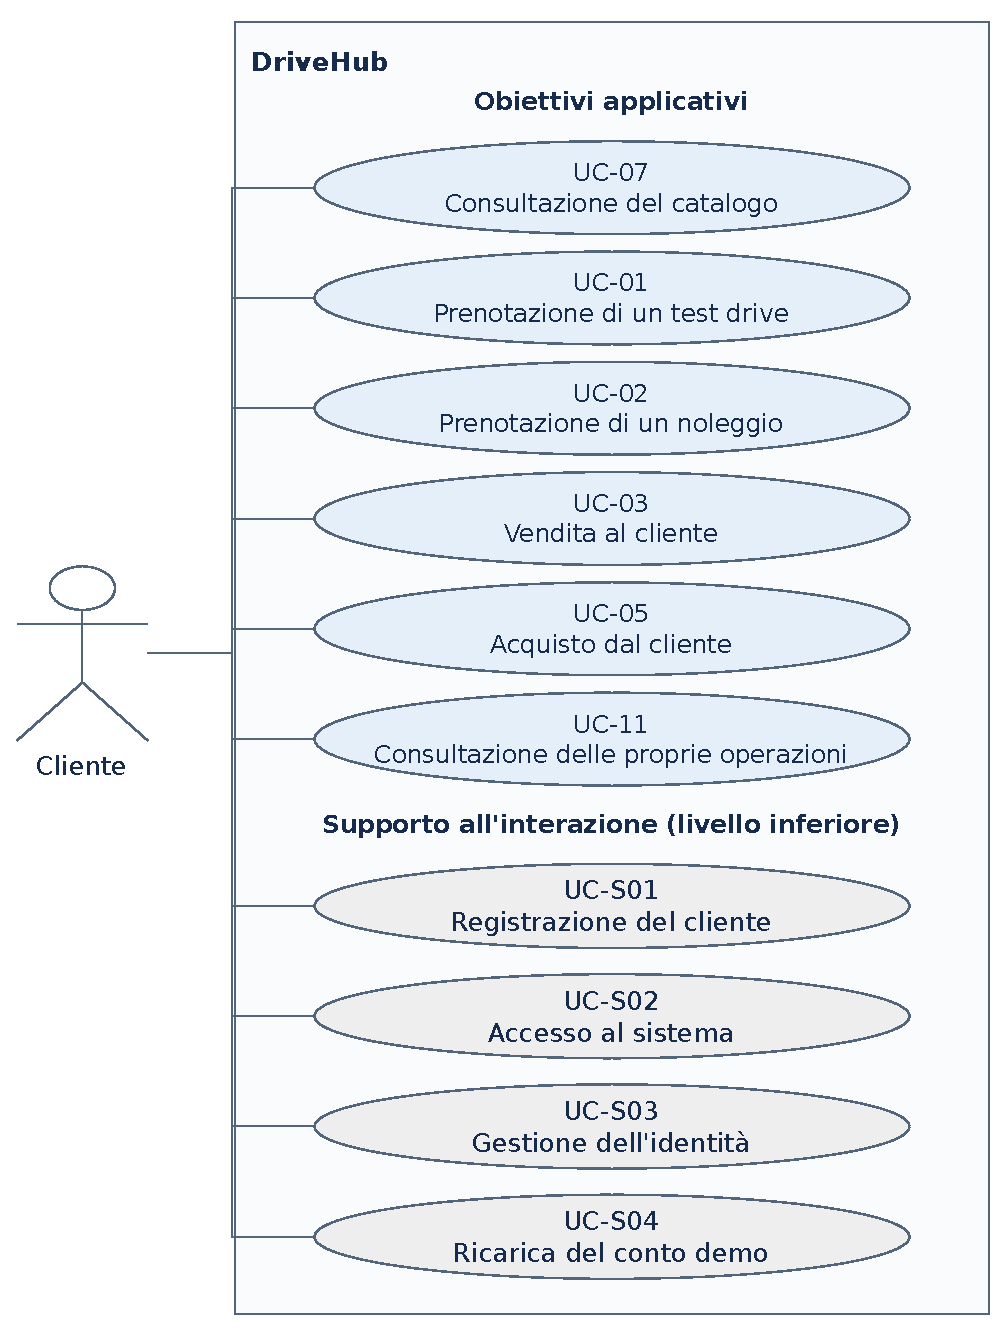
\includegraphics[width=\linewidth,height=.72\textheight,keepaspectratio]{diagrammi/casi-uso-cliente.drawio.pdf}
\caption{Cliente: obiettivi commerciali e consultazioni; in grigio le funzioni di supporto. UC-03 e UC-05 richiedono anche la partecipazione del venditore.}\label{fig:uc-cliente}
\end{figure}
\clearpage
\begin{figure}[!htbp]\centering
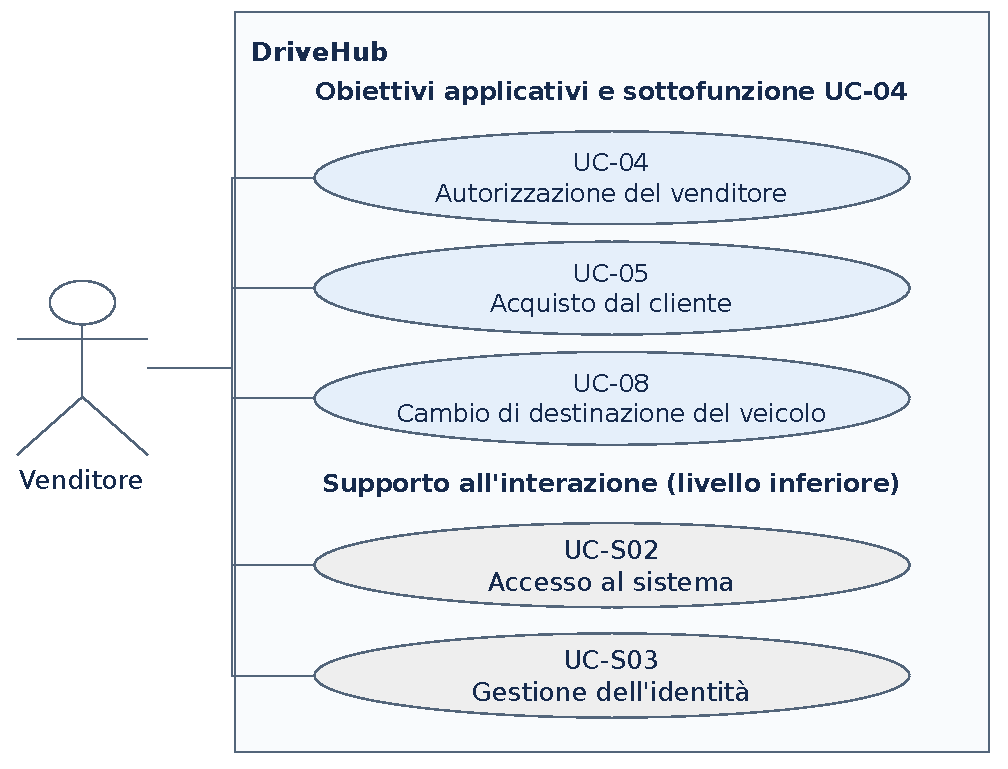
\includegraphics[width=.85\linewidth,height=.67\textheight,keepaspectratio]{diagrammi/casi-uso-venditore.drawio.pdf}
\caption{Venditore: autorizzazione della vendita al cliente (UC-04), esito dell'acquisto dal cliente (UC-05) e destinazione dell'inventario (UC-08).}\label{fig:uc-venditore}
\end{figure}
\begin{figure}[!htbp]\centering
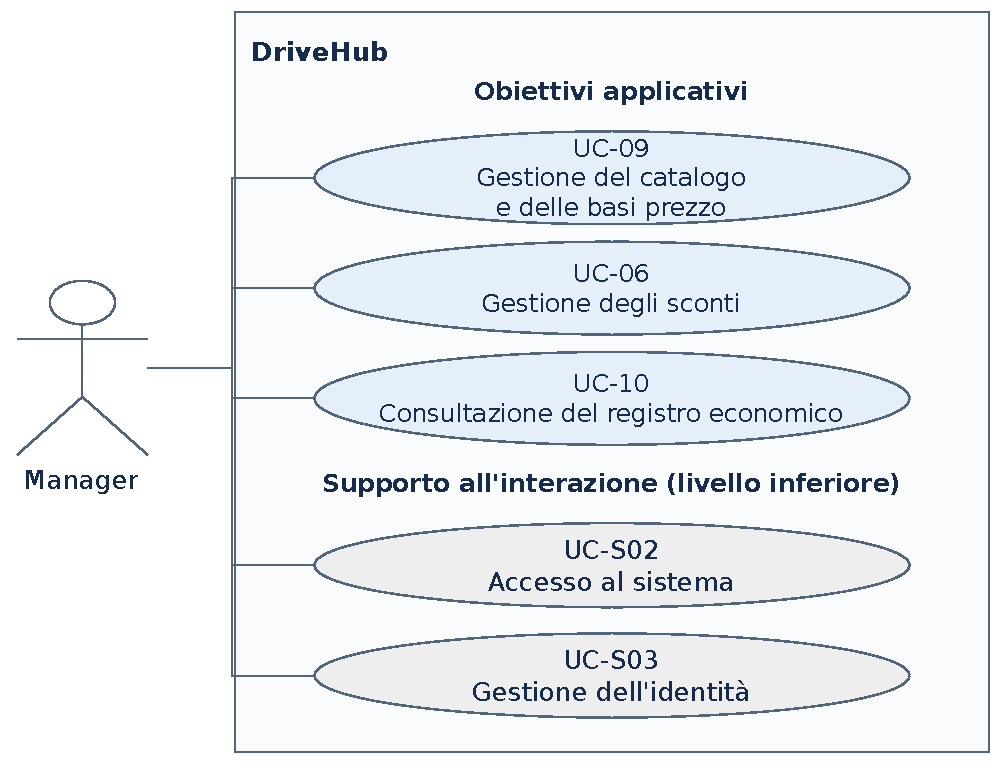
\includegraphics[width=.85\linewidth,height=.67\textheight,keepaspectratio]{diagrammi/casi-uso-manager.drawio.pdf}
\caption{Manager: manutenzione commerciale e consultazione del registro. Le identit\`a staff esistono gi\`a; non vi \`e una registrazione pubblica del personale.}\label{fig:uc-manager}
\end{figure}
\clearpage

\section{Template dei casi principali}\label{sec:template}
Le sei schede complete seguono il percorso originale: test drive, noleggio,
vendita al cliente, cessione, autorizzazione e sconti. UC-05 precede UC-04
nell'esposizione e conserva il proprio identificativo. Le nove schede
aggiuntive sono nell'appendice~\ref{app:casi-uso}.
\begingroup
\small
\setlist{itemsep=1pt,topsep=2pt}
% Schede riscontrate sul codice corrente; non costituiscono esiti di test.
\newcommand{\scheda}[7]{%
  \subsection{\texorpdfstring{\raggedright #1 --- #2}{#1 --- #2}}\label{uc:#1}
  \begin{longtable}{|p{.20\linewidth}|p{.72\linewidth}|}
  \caption{Scheda del caso d'uso #1}\\\hline
  \textbf{Campo} & \textbf{Contenuto}\\\hline\endfirsthead
  \textbf{Campo} & \textbf{Contenuto (continua)}\\\hline\endhead
  Identificativo & #1\\\hline
  Descrizione & #3\\\hline
  Livello & #4\\\hline
  Attori & #5\\\hline
  Precondizioni & #6\\\hline
  Postcondizioni & #7\\\hline
  \end{longtable}
}
\newcommand{\principale}{\paragraph{Flusso principale}}
\newcommand{\alternative}{\paragraph{Alternative}}

Ogni titolo riporta identificativo stabile e denominazione. Le alternative
\emph{n.a}, \emph{n.b} si diramano dal passo \emph{n} della stessa scheda;
si indica se il caso riprende o termina. O indica un obiettivo applicativo,
F una sottofunzione applicativa e S una funzione di supporto. Sono livelli
descrittivi, non livelli di autorizzazione. Gli attori sono ruoli dell'interfaccia;
non si assume un controllo dei permessi indipendente in ogni servizio.
Le postcondizioni descrivono il successo; in caso di errore transazionale
le scritture della singola operazione vengono annullate. Un errore successivo
nell'aggiornamento della vista non annulla un'operazione gi\`a confermata.


Le prove richiamate sono sorgenti e risultati storici, non nuove esecuzioni.
\clearpage
\scheda{UC-01}{Prenotare un test drive}
{Il cliente riserva un giro di prova di un'ora su un veicolo della concessionaria.}
{O --- obiettivo applicativo.}
{Cliente; indirettamente altri clienti con prenotazioni concorrenti.}
{Cliente autenticato; veicolo visibile nel catalogo vendita o noleggio.}
{Prenotazione associata a cliente, veicolo e data/ora; nessun addebito.}
\principale
\begin{enumerate}
\item Il cliente seleziona un veicolo in \emph{Auto in Vendita} o \emph{Auto a Noleggio}.
\item Apre \emph{Prenota Test Drive}, sceglie data e ora iniziale e conferma.
      La UI propone ore intere dalle 09:00 alle 16:00.
\item Il servizio rilegge il veicolo, ammette solo \code{SALE}/\code{RENT},
      controlla che l'istante non sia passato, che il cliente abbia meno di tre
      test drive attivi e che slot e giorno non siano occupati da test drive o noleggi incompatibili.
\item Il sistema salva la prenotazione nella transazione e aggiorna \emph{Le Mie Operazioni}.
\item Il cliente legge la conferma con data e ora del giro di prova.
\end{enumerate}
\alternative
\begin{description}
\item[2.a] Annullamento del dialogo: nessuna prenotazione; termina.
\item[3.a] Data passata, stato cambiato, limite raggiunto o indisponibilit\`a:
  errore, nessuna nuova prenotazione; il cliente pu\`o ripartire da 1 o 2.
\item[4.a] Errore di persistenza: rollback della prenotazione; termina senza successo.
\item[5.a] Successivamente il cliente seleziona un proprio test drive in
  \emph{Le Mie Operazioni} e lo annulla: viene rimosso e la tabella aggiornata.
  Un identificativo non appartenente al cliente viene rifiutato.
\item[5.b] Un successivo noleggio o completamento di vendita sul veicolo
  cancella tutti i suoi test drive futuri, anche fuori dal periodo noleggiato.
  Lo storico rimane; la cancellazione partecipa alla transazione commerciale.
\end{description}
\begin{flushleft}\textbf{Riscontro:} \code{TestDriveService}, \code{TestDriveCancellationObserver},
\code{ClientDashboardView}. La durata \`e una convenzione del giro di prova;
la UI seleziona ore intere, senza attribuire al servizio un vincolo generale
sui minuti che il codice non applica per tutte le ore.\end{flushleft}


\begin{flushleft}\noindent\textbf{Prove e portata:} \code{BookingRulesTest} (fascia e date), \code{BookingConcurrencyIntegrationTest} (limite, slot concorrenti e rollback), \code{TestDriveCancellationIntegrationTest} (cancellazioni); evidenze storiche \code{r06-bookings}/\code{r11-integrated}.\end{flushleft}
\clearpage
\scheda{UC-02}{Noleggiare un veicolo}
{La concessionaria prenota un proprio veicolo al cliente e incassa subito il costo del periodo.}
{O --- obiettivo applicativo.}
{Cliente; clienti titolari di test drive futuri sul medesimo veicolo.}
{Cliente autenticato con conto demo; veicolo presente nel catalogo noleggio.}
{Noleggio salvato e costo intero addebitato; test drive futuri del veicolo cancellati;
il veicolo conserva la destinazione \code{RENT}.}
\principale
\begin{enumerate}
\item Il cliente seleziona un veicolo in \emph{Auto a Noleggio} e apre \emph{Prenota Noleggio}.
\item Sceglie inizio e fine; il dialogo mostra il costo del periodo con estremi inclusi.
\item Conferma. Il servizio rilegge stato, disponibilit\`a e prezzo: inizio non passato,
      fine non precedente all'inizio, stato \code{RENT}, nessuna sovrapposizione.
\item Il sistema verifica il conto e addebita il 100\% del costo ricalcolato.
\item Salva il noleggio e cancella tutti i test drive futuri del veicolo,
      anche oltre il periodo prenotato, nella stessa transazione.
\item Mostra la conferma e aggiorna saldo e operazioni del cliente.
\end{enumerate}
\alternative
\begin{description}
\item[2.a] Date incomplete o invertite: il preventivo non \`e valido;
  il cliente corregge il periodo al passo 2 oppure annulla senza effetti.
\item[3.a] Stato cambiato o periodo gi\`a occupato, anche per una prenotazione concorrente:
  rifiuto senza addebito; ripartire da 1 o 2.
\item[4.a] Conto assente o saldo insufficiente: nessun noleggio e nessun addebito; termina.
\item[5.a] Errore nel salvataggio o nelle cancellazioni collegate: rollback
  anche dell'addebito; nessun successo parziale.
\item[6.a] In seguito UC-08 destina il veicolo alla vendita: se non vi sono
  noleggi in corso, quelli con inizio futuro sono rimossi e rimborsati al 100\%.
  Il cliente vede l'effetto ricaricando le proprie operazioni.
\end{description}
\begin{flushleft}\textbf{Riscontro:} \code{RentalService}, \code{PriceCalculatorService},
\code{TestDriveCancellationObserver}. Il preventivo non \`e un accordo fissato:
il costo viene ricalcolato alla prenotazione. La UI non offre una cancellazione
autonoma del noleggio al cliente.\end{flushleft}


\begin{flushleft}\noindent\textbf{Prove e portata:} \code{BookingConcurrencyIntegrationTest} (conflitti e addebito), \code{TestDriveCancellationIntegrationTest} (rollback Observer), \code{VehicleDestinationIntegrationTest} (rimborsi); evidenze \code{r06-bookings}/\code{r06-destination}/\code{r11-integrated}.\end{flushleft}
\clearpage
\scheda{UC-03}{Richiedere e completare una vendita al cliente}
{La concessionaria vende un veicolo: acconto, autorizzazione del venditore e saldo del totale concordato.}
{O --- obiettivo applicativo articolato in pi\`u sessioni.}
{Cliente principale; venditore per UC-04.}
{Cliente autenticato con conto demo; veicolo proposto in vendita.}
{Nel successo completo: totale registrato come vendita al cliente,
richiesta rimossa, veicolo \code{SOLD}; test drive futuri cancellati.
Dopo il solo acconto: richiesta \code{SALE} aperta, totale fissato e veicolo \code{BLOCKED}.}
\principale
\begin{enumerate}
\item Il cliente seleziona il veicolo in \emph{Auto in Vendita} e avvia l'acquisto.
\item Legge prezzo indicativo e acconto del 20\% nel dialogo e conferma.
\item Il servizio riserva il veicolo solo se ancora \code{SALE}, ricalcola il prezzo,
  addebita l'acconto e salva la richiesta con totale concordato, senza venditore n\'e scadenza.
\item Il venditore approva la richiesta attraverso UC-04, fissando il termine di un mese.
\item Il cliente seleziona la richiesta approvata in \emph{Le Mie Operazioni},
  apre il pagamento del saldo e conferma il residuo del totale concordato.
\item Il servizio verifica autorizzazione e scadenza, addebita il residuo,
  registra l'intero totale nel registro, elimina la richiesta e porta il veicolo a \code{SOLD}.
  Cancella i test drive futuri nella stessa transazione del saldo.
\end{enumerate}
\alternative
\begin{description}
\item[2.a] Annullamento: il veicolo non viene riservato; termina.
\item[3.a] Veicolo non pi\`u disponibile, conto assente o fondi insufficienti:
  rollback di acconto, richiesta e stato; termina.
\item[4.a] Rifiuto del venditore: rimborso integrale dell'acconto,
  richiesta eliminata e veicolo di nuovo \code{SALE}; termina.
\item[5.a] Richiesta non autorizzata o gi\`a scaduta: il saldo viene rifiutato.
  Annullare il dialogo lascia invece aperta la richiesta.
\item[6.a] Saldo insufficiente o errore transazionale: nessuna vendita completata;
  restano acconto e richiesta precedenti; il cliente pu\`o riprovare entro il termine.
\item[6.b] Mancato saldo entro il termine: all'accesso successivo il controllo
  delle scadenze trattiene il 20\% dell'acconto come penale, restituisce il resto,
  rimuove la richiesta e libera il veicolo per la vendita. Non \`e un processo periodico in background.
\end{description}
\begin{flushleft}\textbf{Riscontro:} \code{PurchaseService}, \code{Request}, ADR 0001.
Acconto e saldo hanno transazioni distinte. Basi e sconti successivi non
modificano il totale gi\`a concordato; la penale \`e il 20\% dell'acconto, non del totale.\end{flushleft}


\begin{flushleft}\noindent\textbf{Prove e portata:} \code{PurchaseAgreementIntegrationTest} (accordo immutato, autorizzazione, scadenza, fondi e rollback), \code{TestDriveCancellationIntegrationTest} (Observer); evidenze \code{r04-agreement}/\code{r11-integrated}.\end{flushleft}
\clearpage
\scheda{UC-05}{Proporre un veicolo alla concessionaria}
{La concessionaria valuta e acquista il veicolo ceduto dal cliente; l'etichetta UI \emph{Vendi la tua Auto} usa il punto di vista del cliente.}
{O --- obiettivo applicativo in due fasi, proposta ed esito.}
{Cliente proponente; venditore che decide.}
{Cliente autenticato; modello gi\`a censito; dati del veicolo disponibili.
Se il VIN \`e noto, stato \code{SOLD}, ultima vendita al proponente e nessuna richiesta aperta.}
{Accettazione: stima accreditata al cliente, acquisto della concessionaria registrato,
richiesta rimossa e veicolo \code{SALE}. Dopo la proposta: veicolo \code{WAITING} e richiesta \code{PURCHASE}.}
\principale
\begin{enumerate}
\item Il cliente apre \emph{Vendi la tua Auto} e indica marchio, modello,
  VIN, targa, chilometri e anno.
\item Pu\`o calcolare il preventivo, basato sul modello e sui dati inseriti.
\item Invia la proposta. Il servizio valida i dati e l'eventuale titolarit\`a
  del VIN noto; crea il veicolo oppure aggiorna quello gi\`a venduto al cliente.
\item Salva il veicolo \code{WAITING} e la richiesta con stima ricalcolata,
  positiva o nulla, senza effettuare pagamenti.
\item Il venditore seleziona la proposta \emph{Acquisto dal cliente} in
  \emph{Richieste in Sospeso} e aziona \emph{Approva Richiesta}.
\item Il sistema accredita la stima memorizzata, registra l'acquisto dal cliente
  con venditore, porta il veicolo a \code{SALE} ed elimina la richiesta,
  nella stessa transazione. La UI mostra l'esito.
\end{enumerate}
\alternative
\begin{description}
\item[2.a] Preventivo non richiesto: il cliente pu\`o passare direttamente a 3;
  il servizio ricalcola comunque la stima all'invio.
\item[3.a] Dati invalidi, anno precedente al modello, VIN occupato o non
  appartenente al proponente, richiesta gi\`a aperta: errore e nessuna nuova proposta;
  correggere al passo 1.
\item[5.a] Rifiuto: nessun accredito; richiesta eliminata.
  Il veicolo senza operazioni associate viene eliminato; con storico torna \code{SOLD}.
\item[6.a] Stima nulla, conto mancante, richiesta non pi\`u valida o errore di persistenza:
  rollback dell'intero esito, senza pagamento o acquisizione parziali.
\end{description}
\begin{flushleft}\textbf{Riscontro:} \code{SaleToDealershipService},
\code{ClientDashboardView}, \code{SalesmanDashboardView}. Il registro conserva
un importo non negativo con tipo acquisto; il suo significato \`e un esborso
per la concessionaria. Non esiste un successivo pagamento a saldo per la cessione.
La proposta ammette una stima nulla, ma il conto rifiuta l'accredito zero:
l'accettazione fallisce con rollback (sezione~\ref{sec:sequenze}).\end{flushleft}


\begin{flushleft}\noindent\textbf{Prove e portata:} \code{SaleProposalIntegrationTest} (titolarità e VIN), \code{SaleOutcomeIntegrationTest} (accredito, storico, concorrenza e rollback); evidenze \code{r05-sale-outcome}/\code{r11-integrated}.\end{flushleft}
\clearpage
\scheda{UC-04}{Autorizzare una richiesta di vendita al cliente}
{Il venditore decide l'esito della richiesta con cui la concessionaria vender\`a un veicolo al cliente.}
{F --- sottofunzione applicativa di UC-03, svolta dal venditore.}
{Venditore principale; cliente destinatario dell'esito.}
{Venditore autenticato; richiesta \code{SALE} in sospeso, con acconto gi\`a versato e veicolo riservato.}
{Approvazione: richiesta attribuita al venditore e scadenza impostata a un mese da oggi;
il saldo resta da pagare e il veicolo rimane \code{BLOCKED}.}
\principale
\begin{enumerate}
\item Il venditore apre \emph{Richieste in Sospeso}.
\item Seleziona una riga \emph{Vendita al cliente}, verificando totale,
  acconto e residuo mostrati nella tabella.
\item Aziona \emph{Approva Richiesta}; non compare una conferma preventiva.
\item Il servizio rilegge la richiesta, verifica che sia \code{SALE},
  assegna il venditore e la scadenza a un mese dalla data corrente.
\item La UI mostra l'esito e ricarica richieste e inventario;
  il cliente potr\`a saldare in UC-03.
\end{enumerate}
\alternative
\begin{description}
\item[2.a] Nessuna riga selezionata: messaggio di selezione mancante; ritorno a 2.
\item[2.b] Riga \emph{Acquisto dal cliente}: non \`e questa autorizzazione;
  la stessa azione conclude la cessione secondo UC-05.
\item[3.a] \emph{Rifiuta Richiesta}: il servizio restituisce l'intero acconto,
  elimina la richiesta e ripristina \code{SALE} nella stessa transazione.
  La vendita non prosegue; nessuna penale.
\item[4.a] Richiesta rimossa o tipo non valido: errore, nessuna nuova autorizzazione;
  il venditore ricarica l'elenco.
\item[4.b] Errore durante l'aggiornamento oppure durante il rimborso di 3.a:
  rollback della decisione; lo stato precedente rimane valido.
\end{description}
\begin{flushleft}\textbf{Riscontro:} \code{SalesmanDashboardView},
\code{PurchaseService.approvePurchase}, \code{PurchaseService.rejectPurchase},
\code{OperationQueryService}. Il caso non registra un nuovo venditore e non
rappresenta l'abilitazione di un account staff. La selezione delle richieste
in sospeso \`e affidata alla query della UI; non si attribuisce al comando
un controllo aggiuntivo contro ogni possibile riapprovazione da un chiamante diverso.\end{flushleft}


\begin{flushleft}\noindent\textbf{Prove e portata:} \code{PurchaseAgreementIntegrationTest} (approvazione e termine), \code{PurchaseConcurrencyIntegrationTest} (rifiuto, rimborso ed esiti concorrenti); l\'assenza di selezione e la riapprovazione non sono certificate da quel test. Evidenze \code{r04-agreement}/\code{r11-integrated}.\end{flushleft}
\clearpage
\scheda{UC-06}{Gestire lo sconto su un veicolo}
{Il manager applica o rimuove una promozione di modello o di singolo veicolo.}
{O --- obiettivo applicativo di gestione commerciale.}
{Manager; clienti interessati ai nuovi prezzi.}
{Manager autenticato; modello o veicolo destinatario gi\`a presente nel catalogo.}
{Sconto salvato o rimosso e tabella aggiornata. I nuovi calcoli usano il massimo
fra sconto modello e veicolo; i totali concordati nelle richieste aperte restano invariati.}
\principale
\begin{enumerate}
\item Il manager apre la scheda \emph{Sconti}.
\item Nel riquadro modello seleziona un modello; nel riquadro veicolo
  inserisce invece l'identificativo del veicolo.
\item Inserisce una percentuale intera tra 0 e 50 e aziona \emph{Salva} nel riquadro scelto.
\item Il servizio valida la percentuale e persiste lo sconto;
  uno sconto gi\`a presente sullo stesso elemento viene aggiornato.
\item La UI mostra la conferma e ricarica le due tabelle degli sconti.
\end{enumerate}
\alternative
\begin{description}
\item[2.a] Modello non selezionato o ID non numerico: errore prima del salvataggio;
  ritorno a 2. Un ID veicolo inesistente viene rifiutato dalla persistenza.
\item[3.a] Percentuale non intera o esterna a 0--50: errore, nessuna modifica; ritorno a 3.
\item[3.b] Il manager seleziona uno sconto esistente e aziona \emph{Rimuovi}:
  il servizio elimina lo sconto e la tabella viene ricaricata.
  Senza selezione l'azione non modifica dati; non compare una conferma preventiva.
\item[4.a] Errore transazionale: nessun nuovo sconto salvato; termina senza successo.
\item[5.a] Un'altra tabella gi\`a aperta mostra ancora il vecchio prezzo:
  ricaricarla con \emph{Aggiorna} oppure riaprire la vista.
  La UI non propaga automaticamente ogni modifica a tutte le dashboard gi\`a aperte.
\end{description}
\begin{flushleft}\textbf{Riscontro:} \code{CatalogService}, \code{Discount},
\code{PriceCalculatorService}, \code{ManagerDashboardView}. Gli sconti non
si sommano. La base manuale del veicolo sostituisce la base del modello nella
stessa formula; non impone un prezzo finale sottratto agli sconti.\end{flushleft}


\begin{flushleft}\noindent\textbf{Prove e portata:} \code{PriceCalculatorServiceTest} (massimo e base manuale), \code{DomainInvariantsTest} (0--50), \code{PriceSelectionIntegrationTest} (persistenza della base); evidenze \code{r03-prices}/\code{r11-integrated}.\end{flushleft}

\endgroup
\clearpage
\noindent\textbf{Tracciabilit\`a verso interfaccia e servizi.}
I nomi UI possono usare il punto di vista del cliente: \emph{Acquista Veicolo}
avvia una vendita della concessionaria, mentre \emph{Vendi la tua Auto}
avvia un acquisto dal cliente. Nelle richieste, \code{SALE} e \code{PURCHASE}
mantengono questi significati. Il registro distingue inoltre \code{PENALTY};
un importo positivo non basta da solo a stabilire la direzione economica.

\begin{description}[style=nextline]\raggedright
\item[UC-01, UC-02 e UC-03.]
\code{ClientDashboardView} apre cataloghi, dialoghi e operazioni;
\code{TestDriveService}, \code{RentalService} e \code{PurchaseService}
eseguono i rispettivi comandi. La dashboard avvia il controllo delle
scadenze all'accesso del cliente, senza un pianificatore periodico.
\item[UC-04 e UC-05.]
\code{SalesmanDashboardView} distingue i due tipi di richiesta.
\code{PurchaseService} governa l'autorizzazione e il saldo della vendita;
\code{SaleToDealershipService} governa proposta ed esito della cessione.
\item[UC-06.]
\code{ManagerDashboardView} usa \code{CatalogService} per gli sconti;
\code{PriceCalculatorService} applica la formula. La base manuale
sostituisce la base del modello nella stessa formula (ADR 0001).
\end{description}

Completano le viste UC-07 (catalogo, scheda~\ref{uc:UC-07}), UC-08
(destinazione, scheda~\ref{uc:UC-08}), UC-09 (manutenzione catalogo e basi,
scheda~\ref{uc:UC-09}), UC-10 (registro, scheda~\ref{uc:UC-10}) e UC-11
(proprie operazioni, scheda~\ref{uc:UC-11}). Il supporto comprende UC-S01
(registrazione, scheda~\ref{uc:UC-S01}), UC-S02 (accesso,
scheda~\ref{uc:UC-S02}), UC-S03 (identit\`a, scheda~\ref{uc:UC-S03}) e
UC-S04 (ricarica demo, scheda~\ref{uc:UC-S04}). Ogni identificativo conserva
lo stesso significato nei diagrammi, nelle schede e nella navigazione.

La separazione delle transazioni spiega gli stati intermedi: dopo l'acconto
la vendita non \`e ancora conclusa; dopo una proposta di cessione il cliente
non \`e ancora pagato. Gli esiti osservati nelle schermate illustrano il
percorso, mentre le regole qui dichiarate derivano anche dal riscontro dei
sorgenti. Non si attribuisce a questo ticket una nuova certificazione della
concorrenza o dei rollback tramite test applicativi.
\clearpage

\section{Mockups}\label{sec:mockups}
Il titolo concordato \`e mantenuto; le figure sono \textbf{screenshot
dell'applicazione JavaFX realmente eseguita il 12 novembre 2026}, non
ricostruzioni grafiche. L'avvio usa \code{App.start}, le viste e il tema
correnti, con rendering software su Xvfb e PostgreSQL 16 dedicato.
I nomi e gli importi provengono dalla fixture dimostrativa. Solo nel database
temporaneo sono state spostate alcune date per mostrare operazioni ancora
valide; schema, demo SQL e archivi operativi non sono stati modificati.
Le immagini originali, a risoluzione piena, sono conservate in
\code{docs/relazione/screenshot}; non sono prove di tutte le alternative.

\newcommand{\schermata}[3]{%
  \begin{figure}[!htbp]\centering
  \includegraphics[width=\linewidth,height=.37\textheight,keepaspectratio]{screenshot/#1.png}
  \caption{#2}\label{fig:#3}
  \end{figure}}

\subsection{Autenticazione}
Accesso comune ai tre ruoli (UC-S02) e registrazione riservata al cliente
(UC-S01); il ruolo deriva dall'identità autenticata.

\subsubsection{Schermata iniziale}
\code{App.start} apre direttamente \code{LoginView}. Non esiste una
Welcome Page separata: \emph{Accedi} e \emph{Registrati} sono le due tab
della stessa vista. All'ingresso non si mostrano cataloghi né si seleziona
un ruolo. La figura~\ref{fig:ui-accesso} documenta anche questo punto del
percorso originale, senza duplicare un'immagine o inventare una pagina.

\subsubsection{Accesso}
Il form raccoglie email e password; \emph{Accedi} invoca \code{AuthService}.
Credenziali accettate aprono la dashboard del sottotipo utente, mentre
un errore lascia la vista di accesso e mostra il messaggio. Non vi è una
scelta pubblica del ruolo. Il logout da ogni dashboard ritorna qui.
\schermata{01-accesso}{Accesso corrente, coincidente con la schermata iniziale: email e password.}{ui-accesso}

\subsubsection{Registrazione}
Il cliente inserisce nome, cognome, email e password.
\emph{Crea Account Cliente} valida i dati, crea identità e conto demo a saldo zero nella
stessa transazione e apre la dashboard cliente. Email già utilizzata o dati
invalidi producono un errore; il form rimane disponibile per la correzione.
Venditori e manager sono predisposti nel DB: il precedente selettore di ruolo
non ha un equivalente corrente.
\schermata{02-registrazione}{Registrazione del solo cliente e creazione congiunta del conto demo.}{ui-registrazione}
\clearpage

\subsection{Area Customer}
Le etichette \emph{Customer} e \emph{Salesman} restano nei titoli concordati;
nel testo si usano cliente e venditore. Le quattro tab sono \emph{Auto in
Vendita}, \emph{Auto a Noleggio}, \emph{Vendi la tua Auto} e \emph{Le Mie Operazioni}.

\subsubsection{Catalogo veicoli}
I due cataloghi mostrano modello, anno, targa/usato, chilometri, base
applicata, prezzo consigliato ed effettivo; per il noleggio si mostra anche
la tariffa iniziale giornaliera. Il cliente seleziona una riga e avvia
acconto, noleggio o test drive con i comandi della tab. \emph{Aggiorna}
rilegge disponibilità e prezzi; il comando commerciale li ricontrolla alla
conferma. Durante le letture asincrone i dati sono disabilitati; un errore
espone \emph{Riprova}. La selezione mancante non avvia l'operazione.
Non si attribuiscono alla vista i vecchi filtri testuali non presenti.
\schermata{03-cliente-catalogo}{Catalogo vendita: selezione, acconto del 20\% e test drive.}{ui-cliente-catalogo}
\schermata{05-cliente-noleggio}{Catalogo noleggio: tariffa iniziale e azioni sul veicolo selezionato.}{ui-cliente-noleggio}
\clearpage

\subsubsection{Vendite al cliente e richieste}
\emph{Le Mie Operazioni} mostra le richieste del cliente con veicolo,
totale concordato, acconto, residuo, autorizzazione e scadenza. Selezionare
la richiesta e confermare il saldo completa UC-03 solo dopo UC-04 e nel
termine. Il servizio usa l'accordo persistito, anche dopo variazioni di
listino; fondi insufficienti lasciano valida la richiesta. Chiudere il
dialogo non annulla l'acconto. Non esiste il vecchio comando del cliente
per annullare autonomamente l'acquisto con penale: rifiuto e scadenza hanno
i percorsi distinti descritti nella scheda. La vista non è un registro
completo delle compravendite concluse; quel registro è del manager.
\schermata{08-cliente-operazioni}{Le Mie Operazioni: richieste, noleggi e test drive del cliente; saldo e annullamento del test drive.}{ui-cliente-operazioni}

\subsubsection{Noleggi e test drive}
Le prenotazioni partono dal catalogo e aprono dialoghi, non una vecchia
scheda unica di inserimento. Il test drive richiede data e ora; la UI
propone ore intere 09:00--16:00. \emph{Conferma} salva senza addebito,
se stato, fascia, limite di tre attivi e conflitti lo consentono.
Il noleggio richiede inizio e fine, mostra un preventivo e addebita il
100\% del costo ricalcolato alla conferma, con estremi inclusi.
Annullare un dialogo non scrive dati. Prenotazioni e annullamento del solo
test drive si trovano in \emph{Le Mie Operazioni}
(figura~\ref{fig:ui-cliente-operazioni}); il cliente non può annullare da
qui un noleggio. Un impegno commerciale cancella tutti i test drive futuri
del veicolo, anche esterni al periodo noleggiato.
\schermata{04-cliente-dialogo-test-drive}{Dialogo del test drive: data, ora iniziale, conferma o annullamento.}{ui-test-drive}
\schermata{06-cliente-dialogo-noleggio}{Dialogo di noleggio: periodo e preventivo, ricalcolato al comando finale.}{ui-noleggio}
\clearpage

\subsubsection{Proposta di cessione del proprio veicolo}
In \emph{Vendi la tua Auto} il cliente sceglie marchio e modello censiti e
inserisce VIN, targa, chilometri e anno. \emph{Calcola Preventivo} mostra la
stima; è facoltativo. \emph{Invia Proposta di Vendita} ricalcola e persiste
la stima con veicolo \code{WAITING} e richiesta \code{PURCHASE}, senza
accredito. Dati invalidi o VIN noto senza titolarità sono rifiutati.
L'esito del venditore conclude UC-05: per la concessionaria è un acquisto
dal cliente. Una stima nulla può essere proposta ma non accreditata.
\schermata{07-cliente-cessione}{Proposta di cessione: dati del veicolo, preventivo e invio al venditore.}{ui-cessione}

\subsubsection{Conto dimostrativo}
Il saldo compare nell'header; il dialogo comune mostra anche IBAN e saldo attuale. \emph{Ricarica Saldo} apre la richiesta di un
importo positivo e aggiorna il saldo dopo la scrittura; un valore invalido
non produce una ricarica. La stessa funzione è una tab del dialogo
\emph{Gestione Account} (figura~\ref{fig:ui-identita}). Non è una scheda
bancaria dedicata: la UI corrente non offre il prelievo autonomo né una
connessione bancaria reale. Il conto serve agli addebiti e accrediti
delle operazioni dimostrative e non conserva un estratto di ogni movimento.

\subsubsection{Profilo}
\emph{Gestione Account} apre \code{AccountManagementDialog}, comune ai
ruoli. Nuova email o nuova password richiedono la password corrente;
il successo aggiorna l'identità e chiude il dialogo, un errore lo lascia
aperto. L'eliminazione richiede password e conferma definitiva; se riesce
ritorna all'accesso. Riferimenti storici possono impedirla; un conto
positivo non è di per sé una protezione dalla cancellazione del cliente.
\schermata{09-cliente-identita}{Dialogo comune di gestione identità: qui aperto dal cliente, con la tab aggiuntiva di ricarica.}{ui-identita}
\clearpage

\subsection{Area Salesman}
Le sole tab sono \emph{Richieste in Sospeso} e \emph{Gestione Stato Inventario}.
La tipologia della riga distingue UC-04 dall'esito di UC-05.

\subsubsection{Proposte di cessione in attesa}
Il venditore seleziona una richiesta \emph{Acquisto dal cliente}
(\code{PURCHASE}) nella tabella comune, riconoscendola dalla tipologia;
non c'è una tab separata né si deve presumere un filtro dedicato.
\emph{Approva Richiesta} accredita la stima persistita, registra l'acquisto
con il venditore e rende il veicolo \code{SALE}. \emph{Rifiuta Richiesta}
non paga: elimina il veicolo nuovo o ripristina \code{SOLD} se ha storico.
Nessuna selezione produce un messaggio; errori nel comando causano rollback.
\schermata{10-venditore-richieste}{Tabella comune delle richieste SALE e PURCHASE, con importi e comandi di esito.}{ui-venditore-richieste}

\subsubsection{Richieste di vendita al cliente}
Nella stessa figura~\ref{fig:ui-venditore-richieste}, la riga \code{SALE}
espone totale, acconto e residuo. \emph{Approva Richiesta} assegna venditore
e termine di un mese; non incassa il saldo. \emph{Rifiuta Richiesta}
rimborsa tutto l'acconto e libera il veicolo, senza penale. Non compare una
conferma preventiva di approvazione/rifiuto. Il cliente completa poi UC-03
nella propria area. La lista mostra le richieste in sospeso; il comando di
approvazione non è una garanzia generale contro la riapprovazione diretta.

\subsubsection{Stato dei veicoli}
Il venditore seleziona nell'inventario un veicolo \code{SALE}/\code{RENT}
e conferma il cambio destinazione. La UI avvisa dei noleggi futuri;
il servizio rilegge sotto lock lo stato effettivo. Un noleggio in corso
impedisce il passaggio a vendita; i futuri sono eliminati e rimborsati
integralmente nella medesima transazione. Non è un editor di ogni stato
del veicolo: riserve, proposte e vendite hanno i propri comandi.
\schermata{11-venditore-inventario}{Inventario e cambio della sola destinazione vendita/noleggio.}{ui-venditore-inventario}

\subsubsection{Panoramica prenotazioni: limite attuale}
La vecchia panoramica di noleggi e test drive del venditore non ha un
equivalente corrente. Le sue due tab non offrono questa consultazione;
le prenotazioni personali sono del cliente. Si conserva il punto del
percorso originale dichiarando il limite, senza una figura storica
presentata come attuale o una nuova funzionalità implicita.

\subsubsection{Profilo}
Il pulsante \emph{Gestione Account} della dashboard apre lo stesso
\code{AccountManagementDialog}: modifica email/password con password
corrente ed eliminazione confermata, senza tab di ricarica. L'apertura
è riscontrata in \code{SalesmanDashboardView.buildUi}; non è stata
acquisita una nuova schermata staff. La figura~\ref{fig:ui-identita}
illustra il dialogo comune nel contesto cliente e non certifica una tab
Profilo separata del venditore. La coppia ID/ruolo indirizza le scritture;
le FK dello storico possono impedire l'eliminazione.
\clearpage

\subsection{Area Manager}
Le cinque tab sono \emph{Marchi}, \emph{Modelli}, \emph{Veicoli},
\emph{Sconti} e \emph{Registro economico}. I form modificano la stessa
vista, senza una pagina di dettaglio separata. L'esposizione segue
parco veicoli, marche/modelli, registro e profilo come nell'originale.

\subsubsection{Parco veicoli}
La tab \emph{Veicoli} mostra catalogo e prezzi. Il form raccoglie modello,
VIN, targa, chilometri, anno, destinazione iniziale \code{SALE}/\code{RENT} e scelta della base; una base manuale sostituisce
quella del modello nella stessa formula (ADR 0001), non il prezzo finale.
La selezione di un veicolo permette inoltre di scegliere modalità e base e usare \emph{Applica base alla selezione}. Inserimento e rimozione aggiornano l'elenco; dati invalidi o riferimenti
incompatibili producono errori. Gli sconti individuali sono oggi nella tab
\emph{Sconti}: ID veicolo e percentuale intera 0--50, con \emph{Salva} e
\emph{Rimuovi}. La rimozione è diretta, senza conferma preventiva.
Il massimo tra sconto veicolo e modello vale per nuovi calcoli; non cambia
un totale già concordato. Una tab già caricata può richiedere \emph{Aggiorna}.
\schermata{14-manager-veicoli}{Parco veicoli: basi applicate e scelta automatica/manuale.}{ui-manager-veicoli}
\schermata{15-manager-sconti}{Tab Sconti: gestione distinta dello sconto sul modello e sul veicolo.}{ui-manager-sconti}
\clearpage

\subsubsection{Marche e modelli}
Le anagrafiche occupano due tab. \emph{Marchi} riceve il nome e offre
aggiunta e rimozione della riga selezionata. \emph{Modelli} richiede marchio,
nome unico, base del modello e anno di rilascio. I comandi aggiornano le
tabelle; selezioni mancanti, anni invalidi e dipendenze esistenti impediscono
le operazioni incompatibili. Lo sconto di modello è gestito nell'altro
riquadro della tab \emph{Sconti} (figura~\ref{fig:ui-manager-sconti}): si
seleziona il modello e si salva o rimuove la percentuale 0--50. Non coincide
con lo sconto sul singolo esemplare e non si somma a esso.
\schermata{12-manager-marchi}{Anagrafica dei marchi: inserimento e rimozione.}{ui-manager-marchi}
\schermata{13-manager-modelli}{Anagrafica dei modelli: marchio, base e anno di rilascio.}{ui-manager-modelli}
\clearpage

\subsubsection{Registro delle operazioni}
La tab di sola consultazione legge le righe del registro: vendita al
cliente \code{SALE}, acquisto dal cliente \code{PURCHASE}, penale
\code{PENALTY}. Il tipo determina la direzione economica; gli importi sono
non negativi, anche quando la concessionaria paga il cliente. Le richieste
aperte non sono vendite concluse e i noleggi non diventano automaticamente
righe di \code{Sale}. \emph{Aggiorna} rilegge i dati; durante il caricamento
sono disabilitati e un errore espone \emph{Riprova}.
\schermata{16-manager-registro}{Registro economico: vendite al cliente, acquisti dal cliente e penali.}{ui-manager-registro}

\subsubsection{Profilo}
\emph{Gestione Account} apre il dialogo condiviso anche dalla dashboard
manager (\code{ManagerDashboardView.buildUi}). Le operazioni richiedono
nuova email/password e password corrente, oppure la conferma definitiva
dell'eliminazione; dopo quest'ultima si torna all'accesso. Non compare
la ricarica riservata ai clienti. Si riusa come illustrazione del componente
comune la figura~\ref{fig:ui-identita}, dichiarandone il contesto cliente:
nessuna scheda Profilo o nuova acquisizione manager è presunta. I limiti
dell'unicità trasversale delle identità sono discussi in 2.8.3.
\clearpage

\section{Page Navigation Diagram}\label{sec:navigazione}
Le figure~\ref{fig:nav-cliente}--\ref{fig:nav-manager} descrivono una
\emph{navigazione desktop}: \code{App} sostituisce la scena dopo l'accesso;
la dashboard usa tab selezionabili liberamente. Le azioni aprono dialoghi
modali oppure aggiornano la stessa scheda. Non sono percorsi URL o pagine web.
Il blu identifica schermate/tab, il bianco i comandi, l'ocra dialoghi o
risultati. Gli identificativi collegano il percorso alle schede in 2.2 e nell'appendice A.

\emph{Disconnetti} torna all'accesso per ogni ruolo. \emph{Gestione Account}
apre modifica email, modifica password ed eliminazione; per il cliente
comprende anche la ricarica del conto demo, disponibile pure nell'header.
Chiudere o annullare un dialogo conserva la schermata chiamante;
l'eliminazione riuscita dell'identit\`a torna all'accesso.
La relativa conferma definitiva non va confusa con le rimozioni dirette del catalogo.

La figura~\ref{fig:nav-autori} riprende il \emph{Page Navigation Diagram}
degli autori: conserva l'accesso, lo smistamento per ruolo e le tre diramazioni.
\code{LoginView} sostituisce la precedente Welcome Page; i riquadri
\emph{Accedi} e \emph{Registrati} sono schede della stessa vista, non
schermate successive. La registrazione riuscita porta direttamente al cliente.
Le dashboard espongono rispettivamente quattro, due e cinque schede;
gestione account e ricarica sono comandi, indicati esplicitamente.
Il foglio A3 conserva la struttura d'insieme; le tavole per ruolo dettagliano
azioni e dialoghi.
\tavolaautori{navigazione-autori}{Navigazione: tavola degli autori corretta, con le tre diramazioni originali}{fig:nav-autori}

\begin{figure}[!htbp]\centering
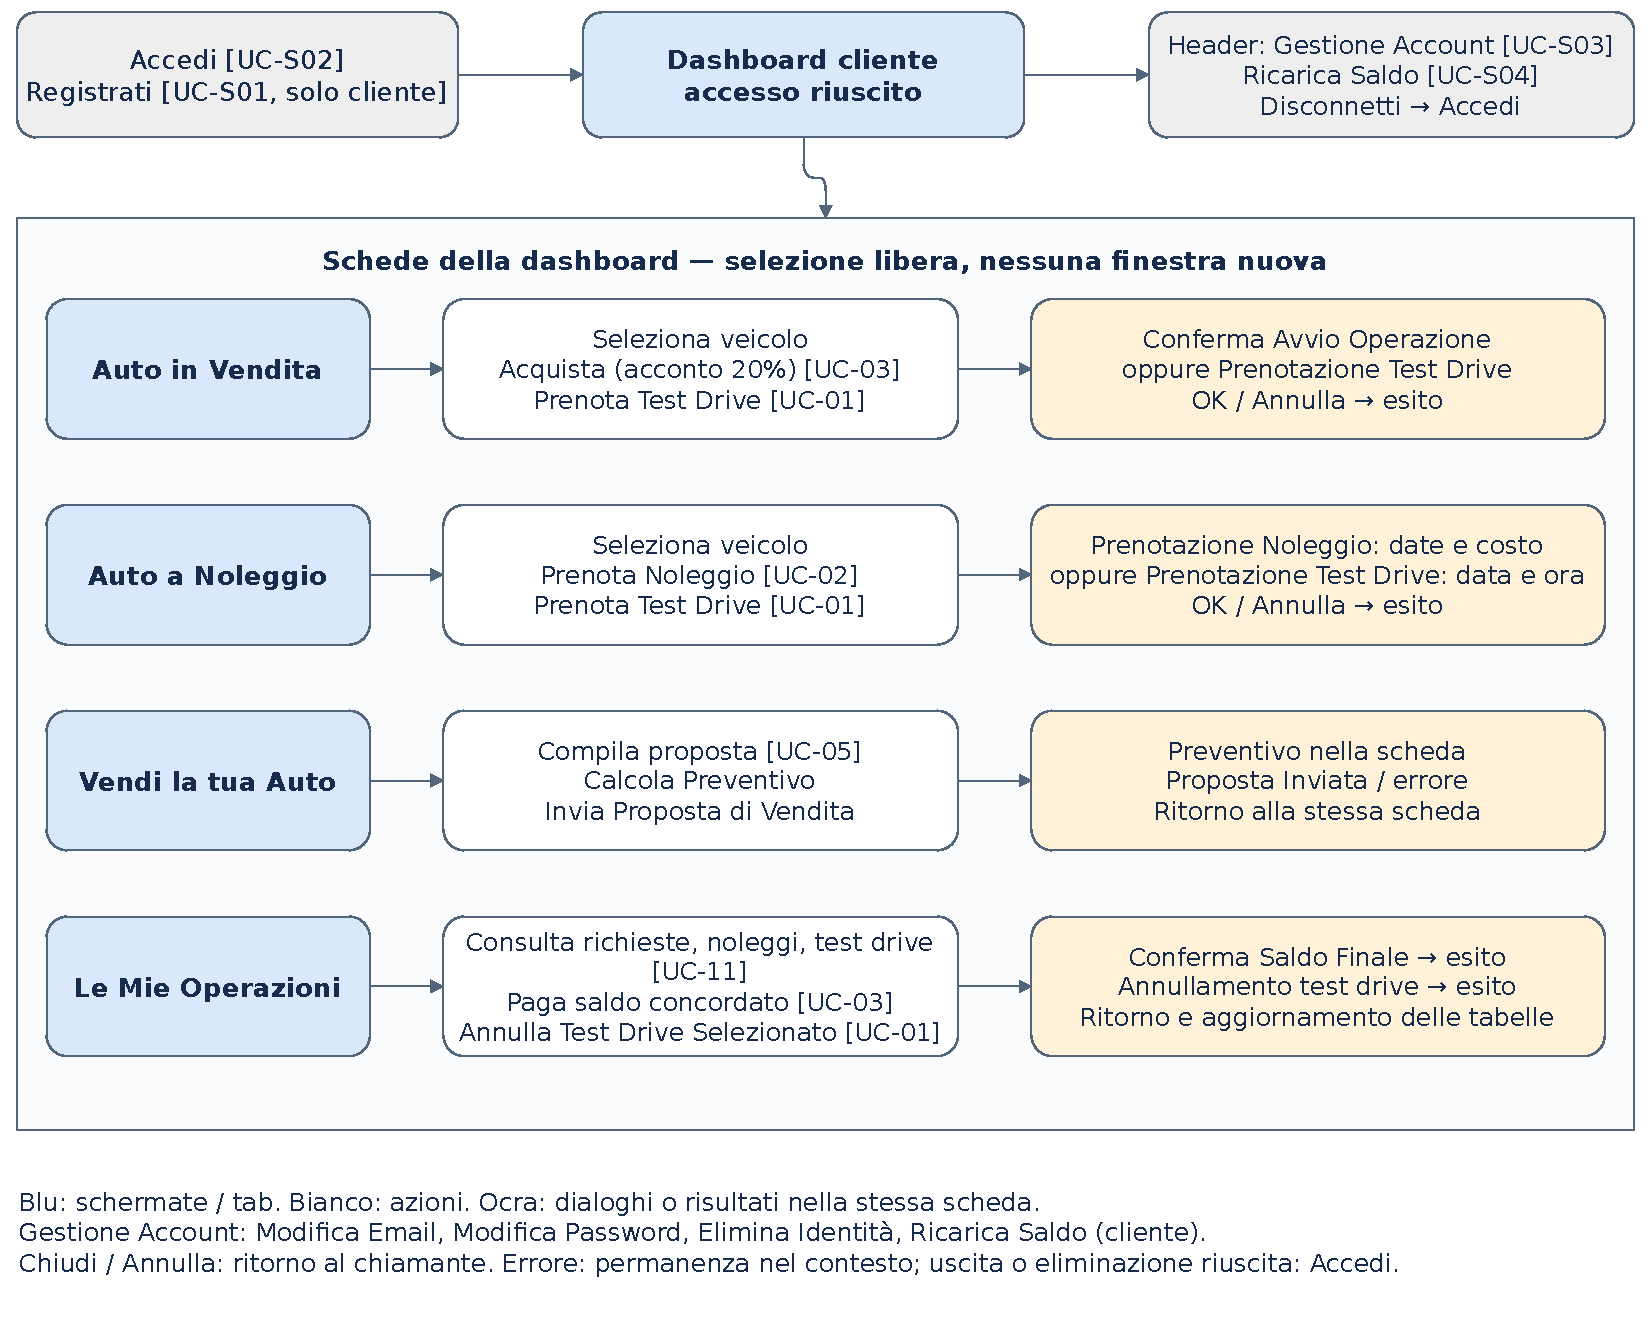
\includegraphics[width=\linewidth,height=.7\textheight,keepaspectratio]{diagrammi/navigazione-cliente.drawio.pdf}
\caption{Navigazione cliente: quattro tab; dialoghi di prenotazione, acconto e saldo; proposta nella scheda; gestione identit\`a e conto. Riscontri visivi nelle figure~\ref{fig:ui-cliente-catalogo}--\ref{fig:ui-identita}.}\label{fig:nav-cliente}
\end{figure}
\clearpage
\begin{figure}[!htbp]\centering
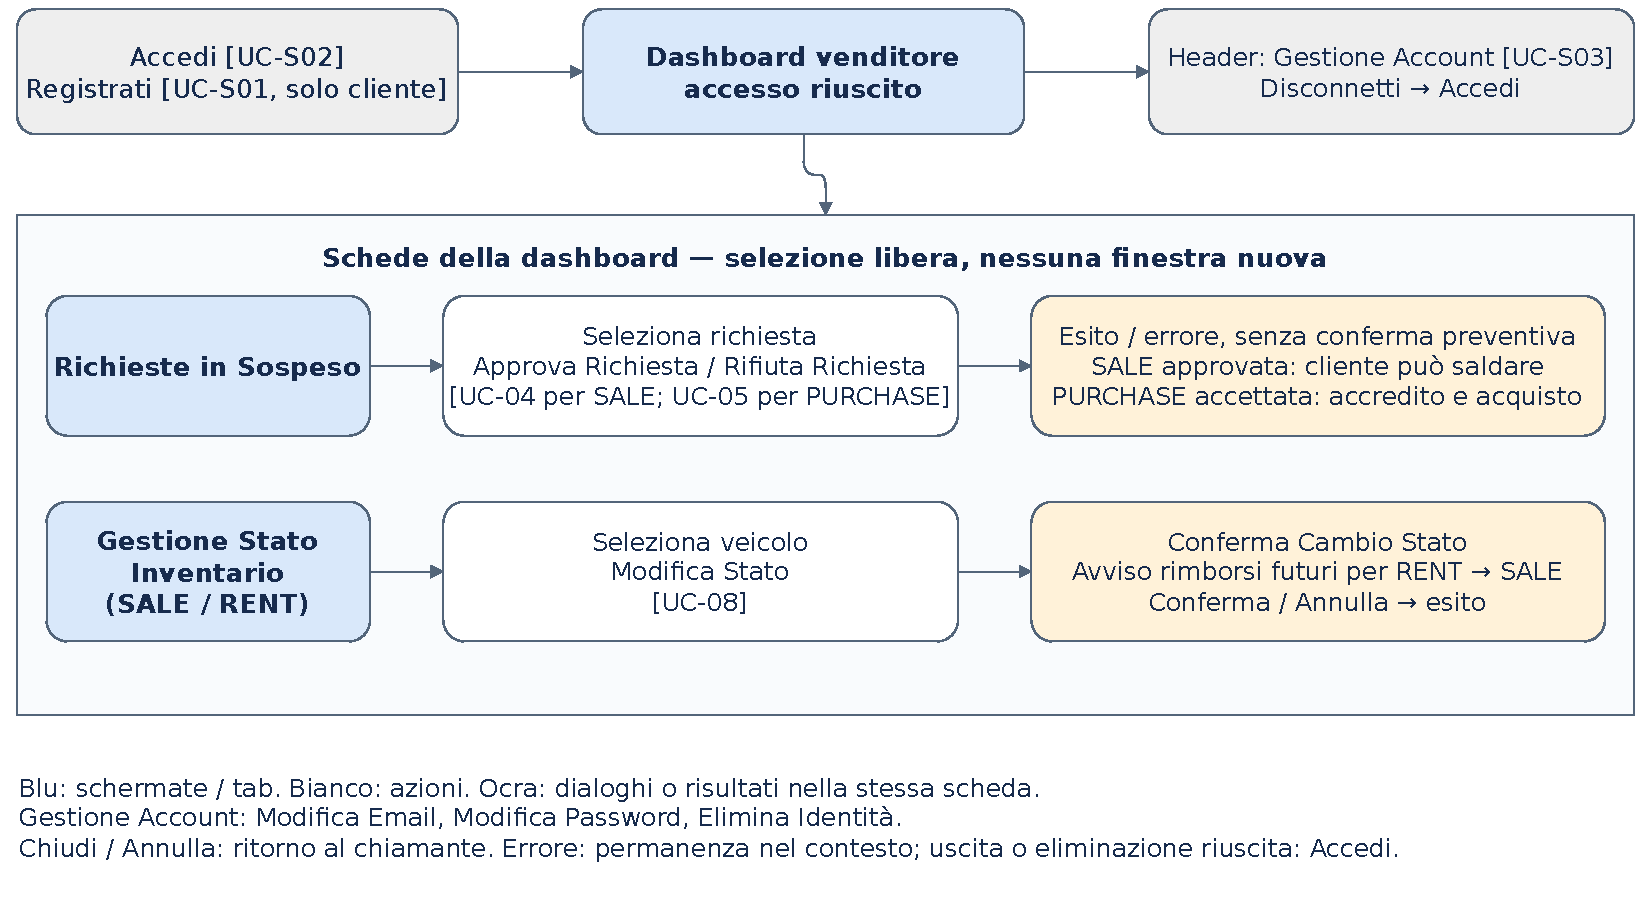
\includegraphics[width=\linewidth,height=.72\textheight,keepaspectratio]{diagrammi/navigazione-venditore.drawio.pdf}
\caption{Navigazione venditore: richieste ed inventario, corrispondenti alle figure~\ref{fig:ui-venditore-richieste} e~\ref{fig:ui-venditore-inventario}. L'approvazione non apre una conferma preventiva; il cambio destinazione s\`i.}\label{fig:nav-venditore}
\end{figure}
Le azioni \emph{Approva Richiesta} e \emph{Rifiuta Richiesta} hanno esiti diversi
secondo il tipo della riga. Una richiesta di vendita al cliente approvata
rimanda il completamento al cliente; l'accettazione di una cessione effettua
subito accredito e acquisto. Il cambio destinazione mostra un avviso dei
noleggi futuri, ma il servizio ne rilegge lo stato prima del commit.
\clearpage
\begin{figure}[!htbp]\centering
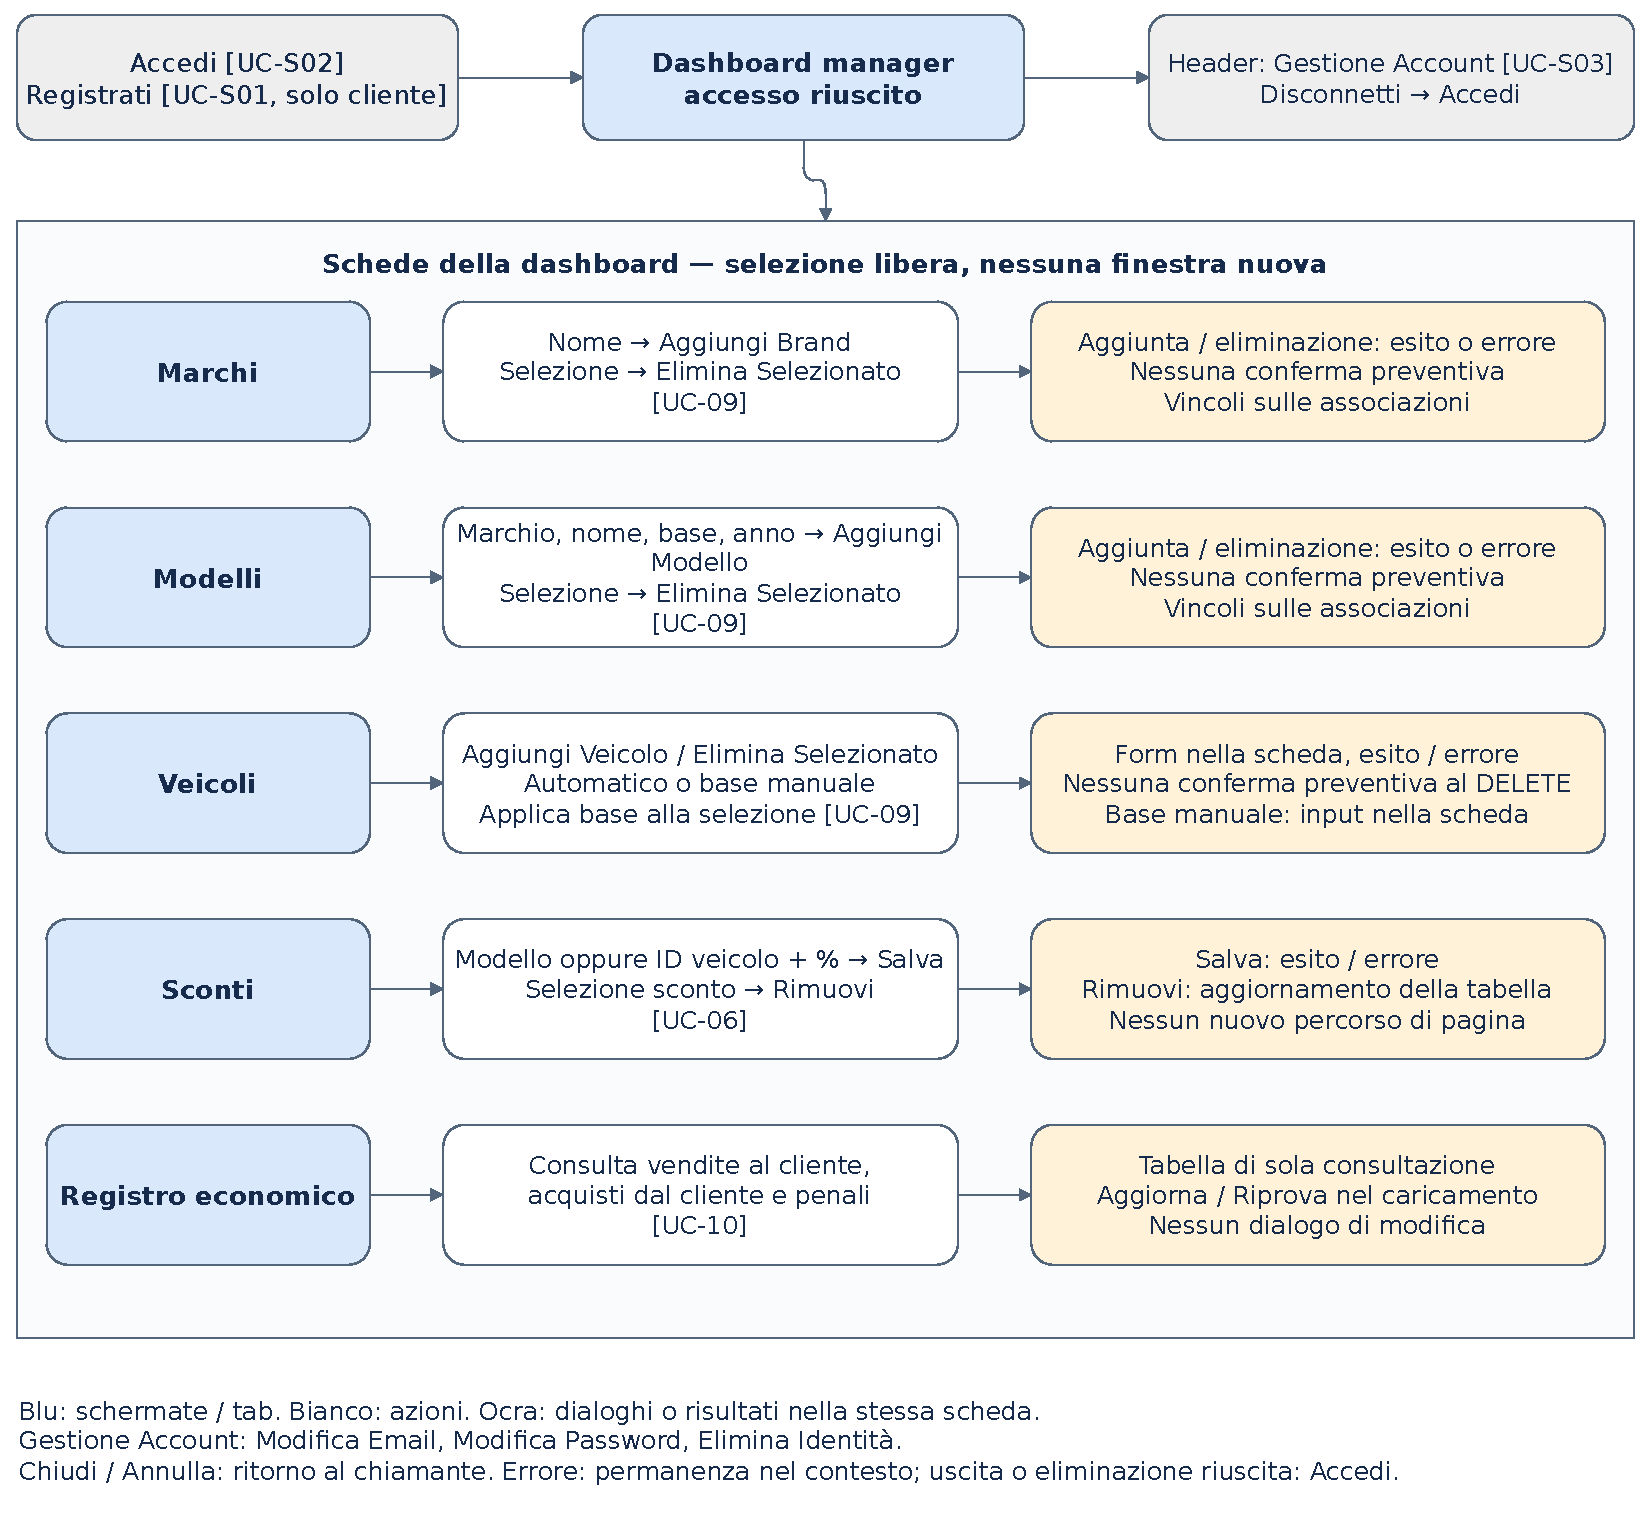
\includegraphics[width=\linewidth,height=.76\textheight,keepaspectratio]{diagrammi/navigazione-manager.drawio.pdf}
\caption{Navigazione manager: cinque tab e form nella stessa vista, corrispondenti alle figure~\ref{fig:ui-manager-marchi}--\ref{fig:ui-manager-registro}. Il registro \`e di sola consultazione.}\label{fig:nav-manager}
\end{figure}
Le rimozioni di catalogo e sconti sono azioni dirette; la vista non aggiunge
una conferma preventiva. Durante le letture asincrone di cataloghi, inventario,
sconti e registro i dati sono disabilitati; in caso di errore compare
\emph{Riprova}. Questo comportamento non va esteso alle letture sincrone
di richieste e operazioni personali. Le nuove tavole sono conservate con
sorgenti \code{.drawio} ed esportazioni PDF in \code{docs/relazione/diagrammi}.
\clearpage

\endgroup

\begingroup
\emergencystretch=6em
\def\UrlBreaks{\do\a\do\b\do\c\do\d\do\e\do\f\do\g\do\h\do\i\do\j\do\k\do\l\do\m\do\n\do\o\do\p\do\q\do\r\do\s\do\t\do\u\do\v\do\w\do\x\do\y\do\z\do\A\do\B\do\C\do\D\do\E\do\F\do\G\do\H\do\I\do\J\do\K\do\L\do\M\do\N\do\O\do\P\do\Q\do\R\do\S\do\T\do\U\do\V\do\W\do\X\do\Y\do\Z}
\section{Package Diagram}\label{sec:package}
L'organizzazione corrente comprende undici package con tipi di produzione.
La figura~\ref{fig:pkg} distingue la composizione dell'applicazione dai suoi
collaboratori: le frecce indicano chi dipende da chi nel codice, non il verso
di restituzione dei dati. I package intermedi \code{domain} e
\code{presentation} non contengono tipi propri e non richiedono viste vuote.

\code{App} avvia JavaFX e collega utente, servizi e callback alle viste;
\code{AppContext} costruisce i DAO PostgreSQL, il gestore delle connessioni,
l'hasher, il publisher con il suo observer e i servizi. Questa composizione
manuale concentra le scelte concrete senza un container. Il contesto riceve
un \code{DatabaseManager}, ma sceglie internamente le implementazioni:
non rende quindi sostituibile ogni dipendenza dal solo costruttore.

\subsection*{Il dominio non dipende dagli altri livelli}
I servizi coordinano i casi d'uso delle sezioni precedenti. Dipendono dai
contratti DAO e dal dominio; i servizi transazionali conoscono anche
\code{DatabaseManager} e JDBC. I DAO definiscono letture, scritture e lock
per risorsa; \code{dao.postgres} ne realizza mapping e SQL. Il dominio
non richiama i DAO e i suoi quattro package non importano gli altri
package applicativi. Ciò non equivale a un isolamento completo dalle
esigenze dell'interfaccia: \code{domain.user} contiene il contratto di
navigazione per ruolo.

\tavolaautori{package-autori}{Package correnti: struttura degli autori e dipendenze attuali}{fig:pkg}
\clearpage

Le dipendenze trasversali limitano una lettura rigidamente a strati.
Le viste usano servizi concreti e tipi del dominio; gli overload di comodo
richiamano il contesto globale, mentre \code{App} passa esplicitamente i
servizi. \code{service} dipende da \code{event}, anche attraverso la
realizzazione dell'observer, ma \code{event} non dipende da \code{service}:
conosce solo il contratto degli osservatori. La connessione JDBC attraversa
questa notifica. \code{security} offre hash e verifica delle password a
\code{AuthService}; non concentra l'autorizzazione di tutte le operazioni.
Le note della tavola completano gli archi selezionati e rendono visibile
anche la dipendenza reciproca tra package di avvio e presentazione.

La separazione evita SQL nelle viste e concentra le formule nel calcolatore,
ma lascia responsabilità ampie nelle dashboard e in \code{AuthService},
che tratta accesso, identità e conto dimostrativo. I contratti che espongono
\code{Connection} facilitano la condivisione della transazione, al prezzo
di legare anche i servizi a JDBC. Non si attribuisce al sistema
un'architettura esagonale o una separazione ideale assente dai sorgenti.

\section{Class Diagram}\label{sec:classi}
Le viste selezionano responsabilità, invarianti e collaborazioni: non sono
cataloghi di tutti i membri. L'appendice~\ref{app:classi} raccoglie le tavole
CL-01--CL-11, con due tavole CL-08a e CL-08b per il package DAO.
Gli identificativi rimangono gli stessi nei rimandi e nei sorgenti draw.io.

La legenda distingue generalizzazione (linea continua e triangolo vuoto),
realizzazione (tratteggio e triangolo), dipendenza (tratteggio e freccia
aperta) e associazione navigabile (linea continua e freccia aperta).
Le molteplicità annotate si riferiscono al solo estremo bersaglio;
l'altro estremo non impone un vincolo numerico. Non sono impiegati rombi
di aggregazione o composizione: un campo o l'iniezione di un collaboratore
non ne dimostrano il ciclo di vita. Gli attributi marcati \code{ID} o
\code{chiave} restano riferimenti scalari, non associazioni a oggetti.

\subsection{Domain Model}
Il dominio separa identità, catalogo, sconti e operazioni. Nella gerarchia
degli utenti, \code{AbstractUser} realizza \code{User}; \code{Client},
\code{Salesman} e \code{Manager} specializzano la parte comune.
\code{Client} può conservare un \code{BankAccount} oppure non averlo ancora
caricato: CL-02 mostra quindi una navigazione verso zero o un conto.
Il conto conserva a sua volta soltanto \code{clientId}; non si disegna
un collegamento inverso a \code{Client}. Il suo comportamento controlla
importi e disponibilità nel modello dimostrativo, non integra una banca.

La figura~\ref{fig:catalogo-corpo} mostra una distinzione utile anche per
UC-03 e UC-09: un veicolo conserva \code{modelId}, mentre riceve un oggetto
\code{Model} quando deve scegliere la base del prezzo. Il primo è un
riferimento per ID; il secondo giustifica una dipendenza di metodo.
Analogamente \code{Model.brand} è una stringa, non un oggetto \code{Brand}.
Stato e modalità del prezzo sono invece attributi tipizzati dagli enum.
La base manuale entra nella stessa formula della base modello, come
stabilito dall'ADR~0001; il totale concordato è un concetto distinto.

\tavolaautori{classi-dominio-insieme}{Domain Model d'insieme: utenti, catalogo, sconti e operazioni}{fig:catalogo-corpo}
\clearpage

CL-04 rende esplicita la sola generalizzazione degli sconti: il limite
intero 0--50 appartiene alla base astratta, mentre le specializzazioni
conservano l'ID del modello o del veicolo. La scelta dello sconto massimo
è responsabilità del servizio di calcolo, non di una relazione tra entità.
CL-05 distingue \code{Request} dal registro \code{Sale} e dalle prenotazioni
\code{Rent}/\code{TestDrive}. Nessuna di queste classi contiene oggetti
cliente o veicolo. Le richieste \code{SALE} conservano totale e acconto
dell'accordo di UC-03; nelle \code{PURCHASE}, relative a UC-05, il campo
\code{deposit} contiene la stima e il totale concordato è assente.
Il tipo del registro distingue vendita al cliente, acquisto dal cliente e penale con importi
non negativi, senza dedurre il significato dal segno.

\subsection{Business Layer}
CL-01 e CL-06 separano composizione e coordinamento. Il contesto conserva
i collaboratori e li passa ai costruttori. I tre servizi dei flussi
economici coordinano i DAO, mentre il calcolatore concentra le formule.
\code{CatalogService} prepara anche righe con nomi e prezzi per le tabelle;
il servizio di interrogazione espone le letture delle operazioni.
I record annidati del catalogo sono dati di lettura, non nuove entità persistenti.

L'observer di cancellazione appartiene a \code{service}, perché applica
la priorità della vendita al cliente e del noleggio sui test drive di UC-01.
Il contratto, il publisher e l'evento risiedono invece in \code{event}.
La figura~\ref{fig:eventi-corpo} comprende la collaborazione di notifica sincrona sulla connessione
del servizio prima del commit: un errore dell'observer deve impedirlo.
La separazione consente altri osservatori, ma non offre consegna asincrona,
persistenza degli eventi o recupero tramite outbox.

\tavolaautori{classi-business-insieme}{Business Layer d'insieme: servizi, calcolo, transazioni, sicurezza ed eventi}{fig:eventi-corpo}
\clearpage

\subsection{DAO}
CL-08a raccoglie dieci contratti distinti per risorsa, senza un gestore
comune da cui ereditare. La classe \code{DatabaseManager} apre connessioni ed esegue il corpo
di una transazione mediante le due callback annidate di CL-08b, tentando
commit oppure rollback in caso di eccezione. Non è un DAO base né un ORM.
Le firme con \code{Connection} rendono visibile la partecipazione di più
scritture alla stessa transazione. Alcuni overload di lettura dei contratti
forniscono però un default che delega alla lettura senza connessione:
la sola firma non basta a garantirne il riuso. I DAO PostgreSQL pertinenti
ridefiniscono tali percorsi.

CL-09 rende riconoscibile ciascuna realizzazione del relativo contratto.
Ogni DAO PostgreSQL conserva il gestore ricevuto dal costruttore: non si
deduce una composizione UML da questo riferimento condiviso. Le letture
autonome gestiscono la propria connessione; quelle transazionali e le
scritture protette usano quella passata dal servizio. Il mapping ricostruisce
le entità e converte i domini enumerati in accordo con l'ADR~0002.
Gli ID che legano i record persistenti non diventano per questo riferimenti
a oggetti nel dominio. I dettagli SQL e i protocolli dei singoli flussi
sono rinviati al capitolo~\ref{ch:implementazione}.


\tavolaautori{classi-dao-insieme}{DAO d'insieme: contratti, realizzazioni PostgreSQL e gestore JDBC}{fig:dao-insieme}
\clearpage

\subsection{Presentation Layer}
CL-10 mostra le viste effettive: accesso e tre dashboard estendono
\code{BorderPane}; il dialogo di gestione dell'identità è una classe di
utilità con metodi statici, non un sottotipo di \code{Dialog}. Le viste
costruiscono controlli JavaFX direttamente, senza controller FXML.
\code{AsyncLoad}, interno al package, usa \code{Task} e worker virtuali
per le letture delle tabelle; pubblica solo il caricamento corrente sul
thread grafico. Ciò non rende asincrone tutte le azioni economiche né
interrompe immediatamente JDBC quando un caricamento è scartato.

La navigazione delle sezioni 2.3--2.4 parte da \code{User}: il suo metodo
\code{openDashboard} viene specializzato nei tre ruoli. Il sottotipo invoca
il metodo specifico del contratto \code{UserDashboardNavigator}.
\code{App} crea un'implementazione anonima
che costruisce la dashboard appropriata. È un double dispatch nello
stile Visitor: aggiungere un ruolo richiede di aggiornare anche il
contratto e il collegamento delle viste. \code{App} non realizza direttamente
quell'interfaccia. Il dominio resta privo di import JavaFX, ma conosce
questa esigenza di navigazione.

CL-11 mostra il confine delle credenziali. Il contratto
\code{PasswordHasher} è ricevuto da \code{AuthService}; la realizzazione
PBKDF2 viene scelta nel contesto.
Questo confine riguarda hash e verifica della password. La scelta della
dashboard per ruolo non equivale a un controllo autonomo dei permessi
in ogni metodo dei servizi, che non ricevono tutti un'identità autenticata.
Non viene quindi attribuita al solo package \code{security} una garanzia
generale di autorizzazione.
\clearpage

\tavolaautori{classi-presentazione-insieme}{Presentazione d'insieme: viste, dialogo comune e navigazione}{fig:presentazione-insieme}
\clearpage

\endgroup

\begingroup
\emergencystretch=6em
\def\UrlBreaks{\do\a\do\b\do\c\do\d\do\e\do\f\do\g\do\h\do\i\do\j\do\k\do\l\do\m\do\n\do\o\do\p\do\q\do\r\do\s\do\t\do\u\do\v\do\w\do\x\do\y\do\z\do\A\do\B\do\C\do\D\do\E\do\F\do\G\do\H\do\I\do\J\do\K\do\L\do\M\do\N\do\O\do\P\do\Q\do\R\do\S\do\T\do\U\do\V\do\W\do\X\do\Y\do\Z}
\section{Sequence Diagram}\label{sec:sequenze}
Le tavole seguono UC-03/UC-04, UC-02 e UC-05, descritti nelle
schede della sezione~\ref{sec:template}. I titoli storici conservano il
punto di vista del cliente; la spiegazione adotta quello della concessionaria:
\emph{vendita al cliente} e \emph{acquisto dal cliente}, anche detto
\emph{cessione del cliente}. Non vengono riproposti gateway, unità di lavoro
o strategie della versione precedente.

Ogni tavola distingue l'azione dell'attore, l'handler JavaFX e la chiamata
al servizio, quindi dettaglia le collaborazioni selezionate. I partecipanti
DAO sono le implementazioni PostgreSQL dei contratti già presentati.
Le frecce continue blu sono chiamate sincrone del percorso principale;
quelle rosse evidenziano un'alternativa, i ritorni espliciti sono tratteggiati.
I frammenti \code{alt}/\code{else} sono mutuamente alternativi; \code{loop}
ripete un episodio e \code{ref} rinvia alla collaborazione comune SQ-OB.
Le diciture \guillemotleft{}azione\guillemotright{}, \guillemotleft{}SQL\guillemotright{}, \guillemotleft{}sintesi\guillemotright{} e \guillemotleft{}memoria\guillemotright{} sono descrittive:
non introducono metodi Java. Le note riassumono chiamate effettive omesse
dalle frecce per contenere il numero di linee di vita.

I parametri \code{vehicleId}, \code{clientId}, \code{requestId} e
\code{salesmanId} sono identificativi; \code{Vehicle}, \code{Request},
\code{Model} e \code{BankAccount} sono invece copie in memoria ottenute o
costruite nel flusso. La selezione nella vista non sostituisce una rilettura
transazionale. Le sigle T1--T7 identificano episodi distinti; i nomi delle connessioni
sono locali alla singola tavola. La lettera
\code{c} indica la \code{Connection} effettivamente passata ai DAO.
\code{DatabaseManager} apre la connessione, disabilita autocommit, esegue
la callback e tenta il commit. Su un'\code{Exception} nel corpo o nel commit
tenta rollback, conserva un eventuale errore di rollback come eccezione
soppressa e propaga una \code{RuntimeException}. Il ritorno normale alla
vista segue il commit; errori di apertura, chiusura o comunicazione non
consentono di promettere recupero da qualsiasi guasto o esito sempre conoscibile.

\subsection{Vendita di un veicolo al cliente}
La tavola d'insieme riprende il flusso originale con i collaboratori attuali;
le viste successive approfondiscono transazioni e alternative.
\tavolaautori{sequenza-vendita-insieme}{Vendita al cliente: acconto, autorizzazione e saldo}{fig:sq-vendita-insieme}
\clearpage

La vendita al cliente si articola in sessioni e transazioni separate.
SQ-01a (figura~\ref{fig:sq01a}) copre l'avvio di UC-03: l'aggiornamento
condizionale da \code{SALE} a \code{BLOCKED} precede il calcolo effettivo.
Il prezzo del dialogo è un'anteprima. Il servizio applica la formula con
la base selezionata, automatica o manuale, e fissa totale e acconto del 20\%
nella richiesta \code{SALE}, insieme all'addebito. Come nell'ADR~0001,
la base manuale non è un prezzo finale imposto. Le letture del modello e
degli sconti aprono però connessioni autonome: avvengono durante la callback,
ma fuori dalla transazione di scrittura T1 e senza uno snapshot unico
del listino. Non si attribuisce loro il lock ottenuto sul veicolo.

\begin{figure}[p]
  \centering
  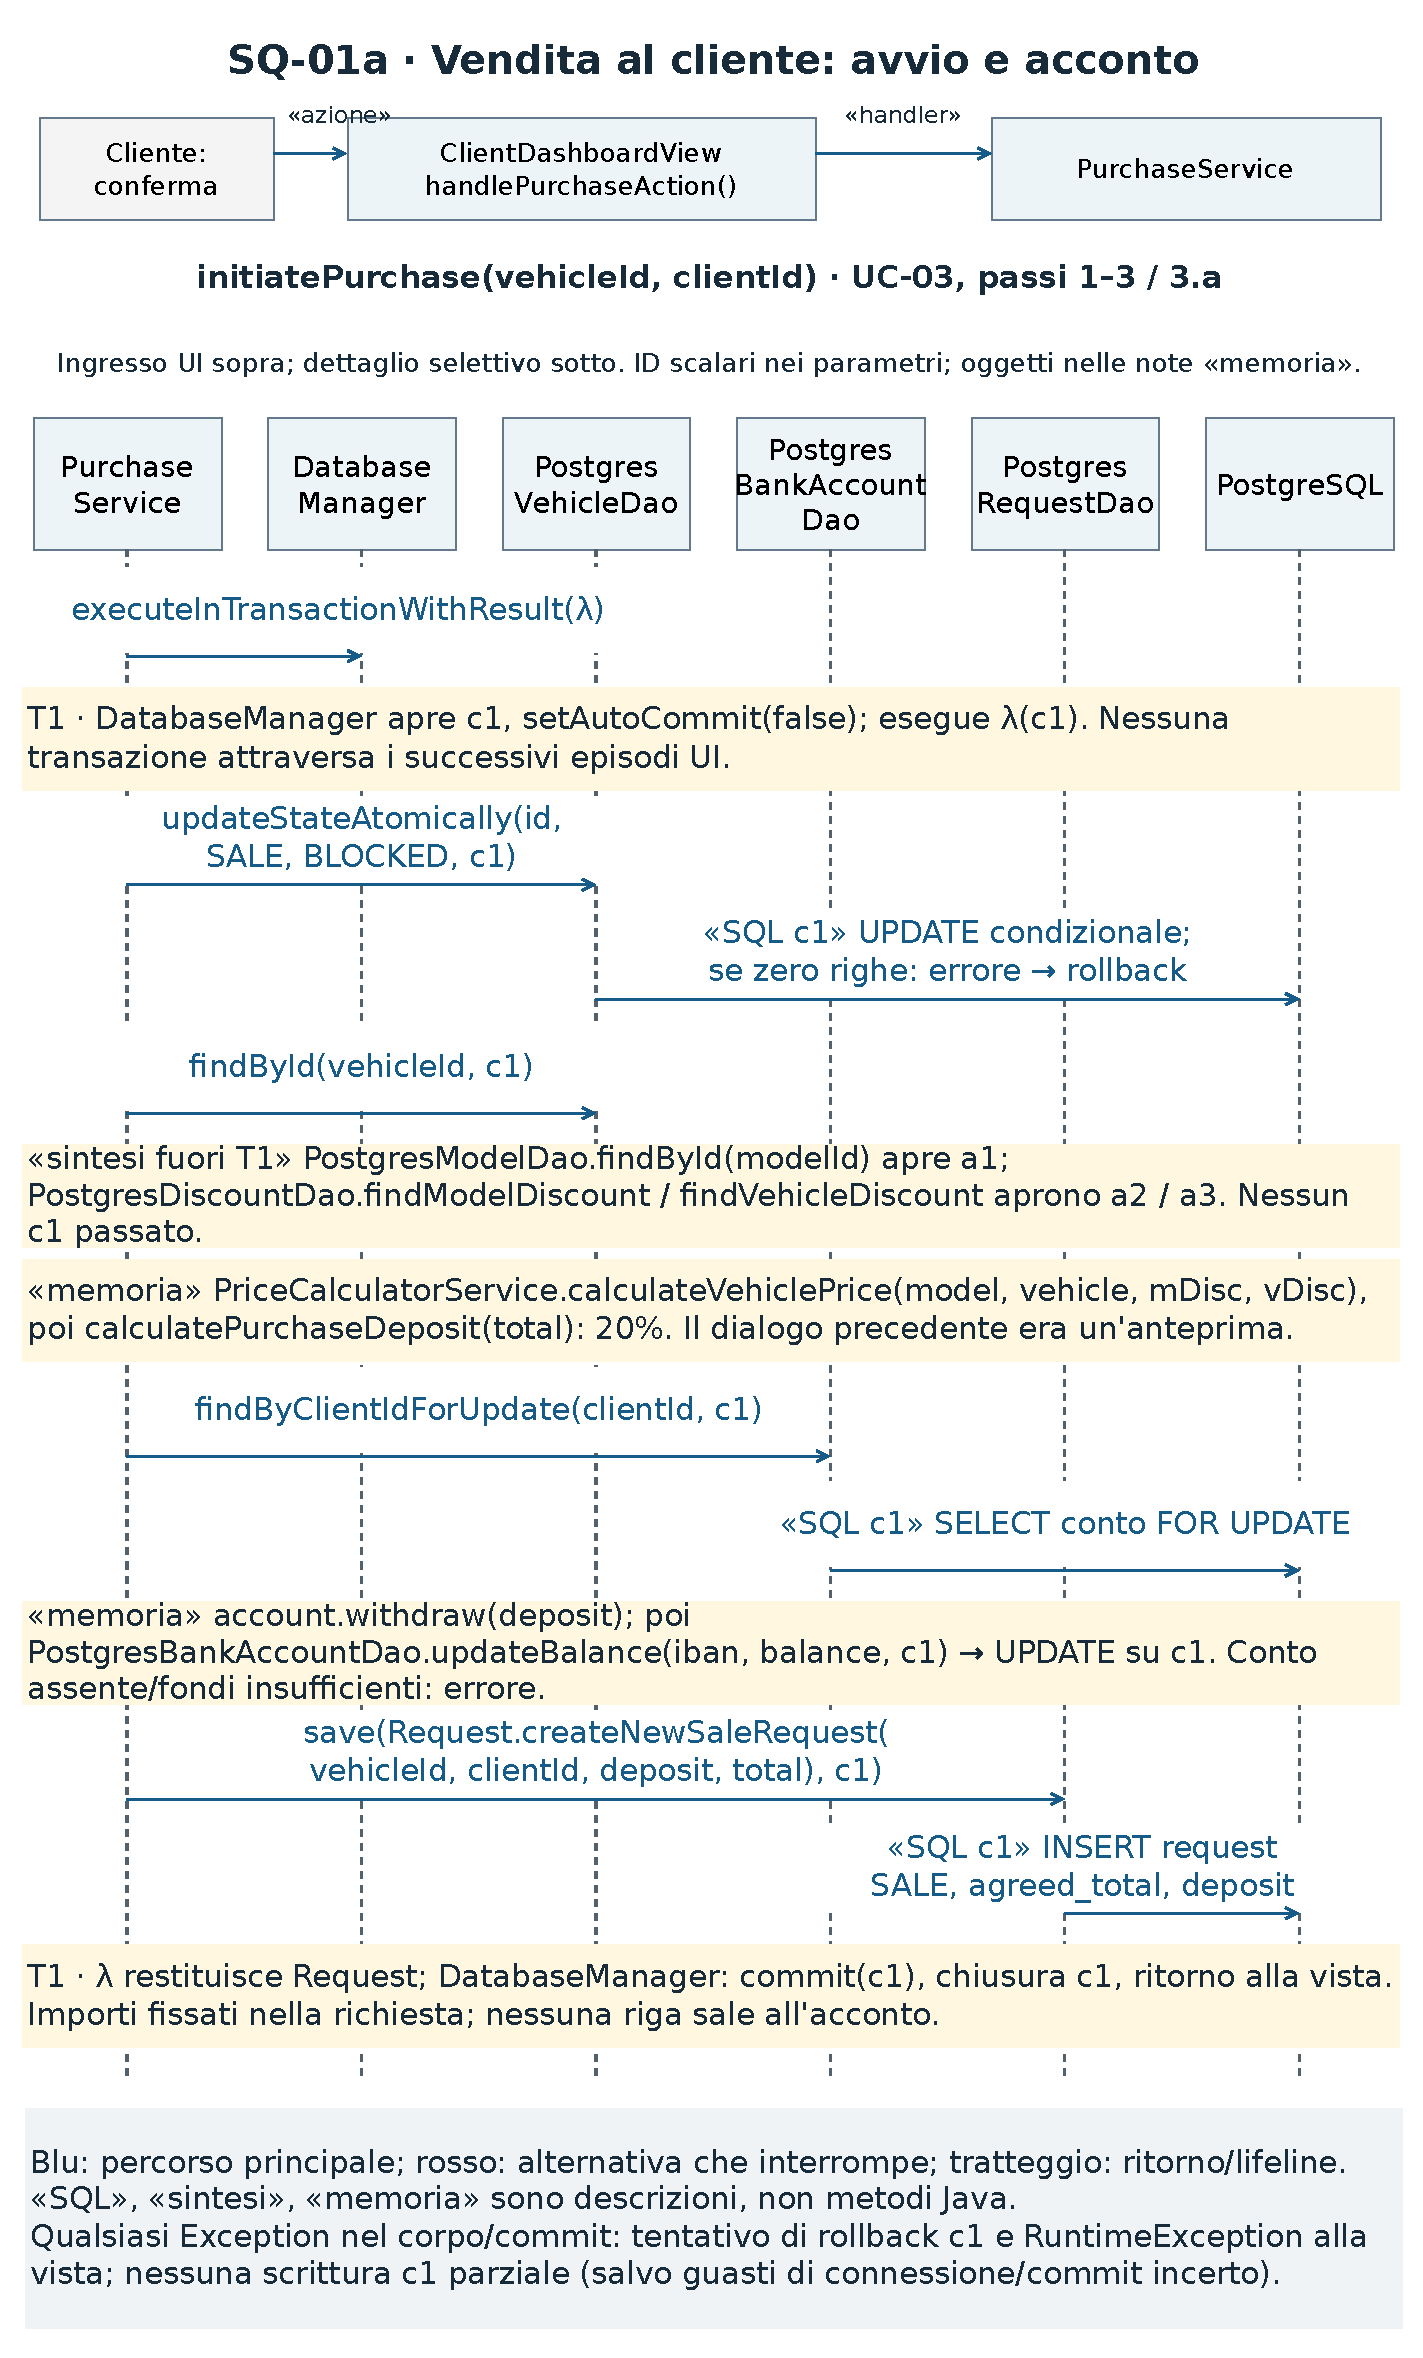
\includegraphics[width=\linewidth,height=.88\textheight,keepaspectratio]{diagrammi/sequenza-vendita-avvio.drawio.pdf}
  \caption{SQ-01a --- Vendita al cliente: avvio, totale concordato e acconto.}\label{fig:sq01a}
\end{figure}
\clearpage

SQ-01b (figura~\ref{fig:sq01b}) rappresenta UC-04: l'approvazione assegna
venditore e scadenza a un mese dalla data corrente, lasciando il veicolo
riservato e il saldo ancora da versare. Il rifiuto restituisce l'intero
acconto, elimina la richiesta e ripristina \code{SALE}. Non crea una penale
né una registrazione nel registro \code{sale}. La richiesta viene riletta
con \texttt{FOR UPDATE}; la lista delle richieste in sospeso è selezionata
dalla UI, mentre il comando non verifica nuovamente che la richiesta non
fosse già approvata. L'autorizzazione di UC-04 è l'esito della richiesta,
non l'abilitazione di un account staff.

SQ-01c (figura~\ref{fig:sq01c}) conclude UC-03. Il servizio rilegge la
richiesta sotto lock, ne controlla tipo, approvazione e scadenza, quindi
addebita \emph{totale concordato meno acconto}, senza ricalcolare il listino.
Il giorno della scadenza è ancora ammesso. Registra l'intero totale come
\code{Sale} di tipo \code{SALE}, elimina la richiesta, porta il veicolo
a \code{SOLD} e notifica sincronicamente l'Observer prima del commit.
Un errore lascia validi gli effetti degli episodi precedenti, come l'acconto
già confermato, e annulla le scritture del solo saldo. I lock coordinano
gli accessi ai record coinvolti; i servizi di saldo ed esito ricevono ID,
senza un'identità del chiamante con cui provare un controllo generale dei permessi.

\begin{figure}[p]
  \centering
  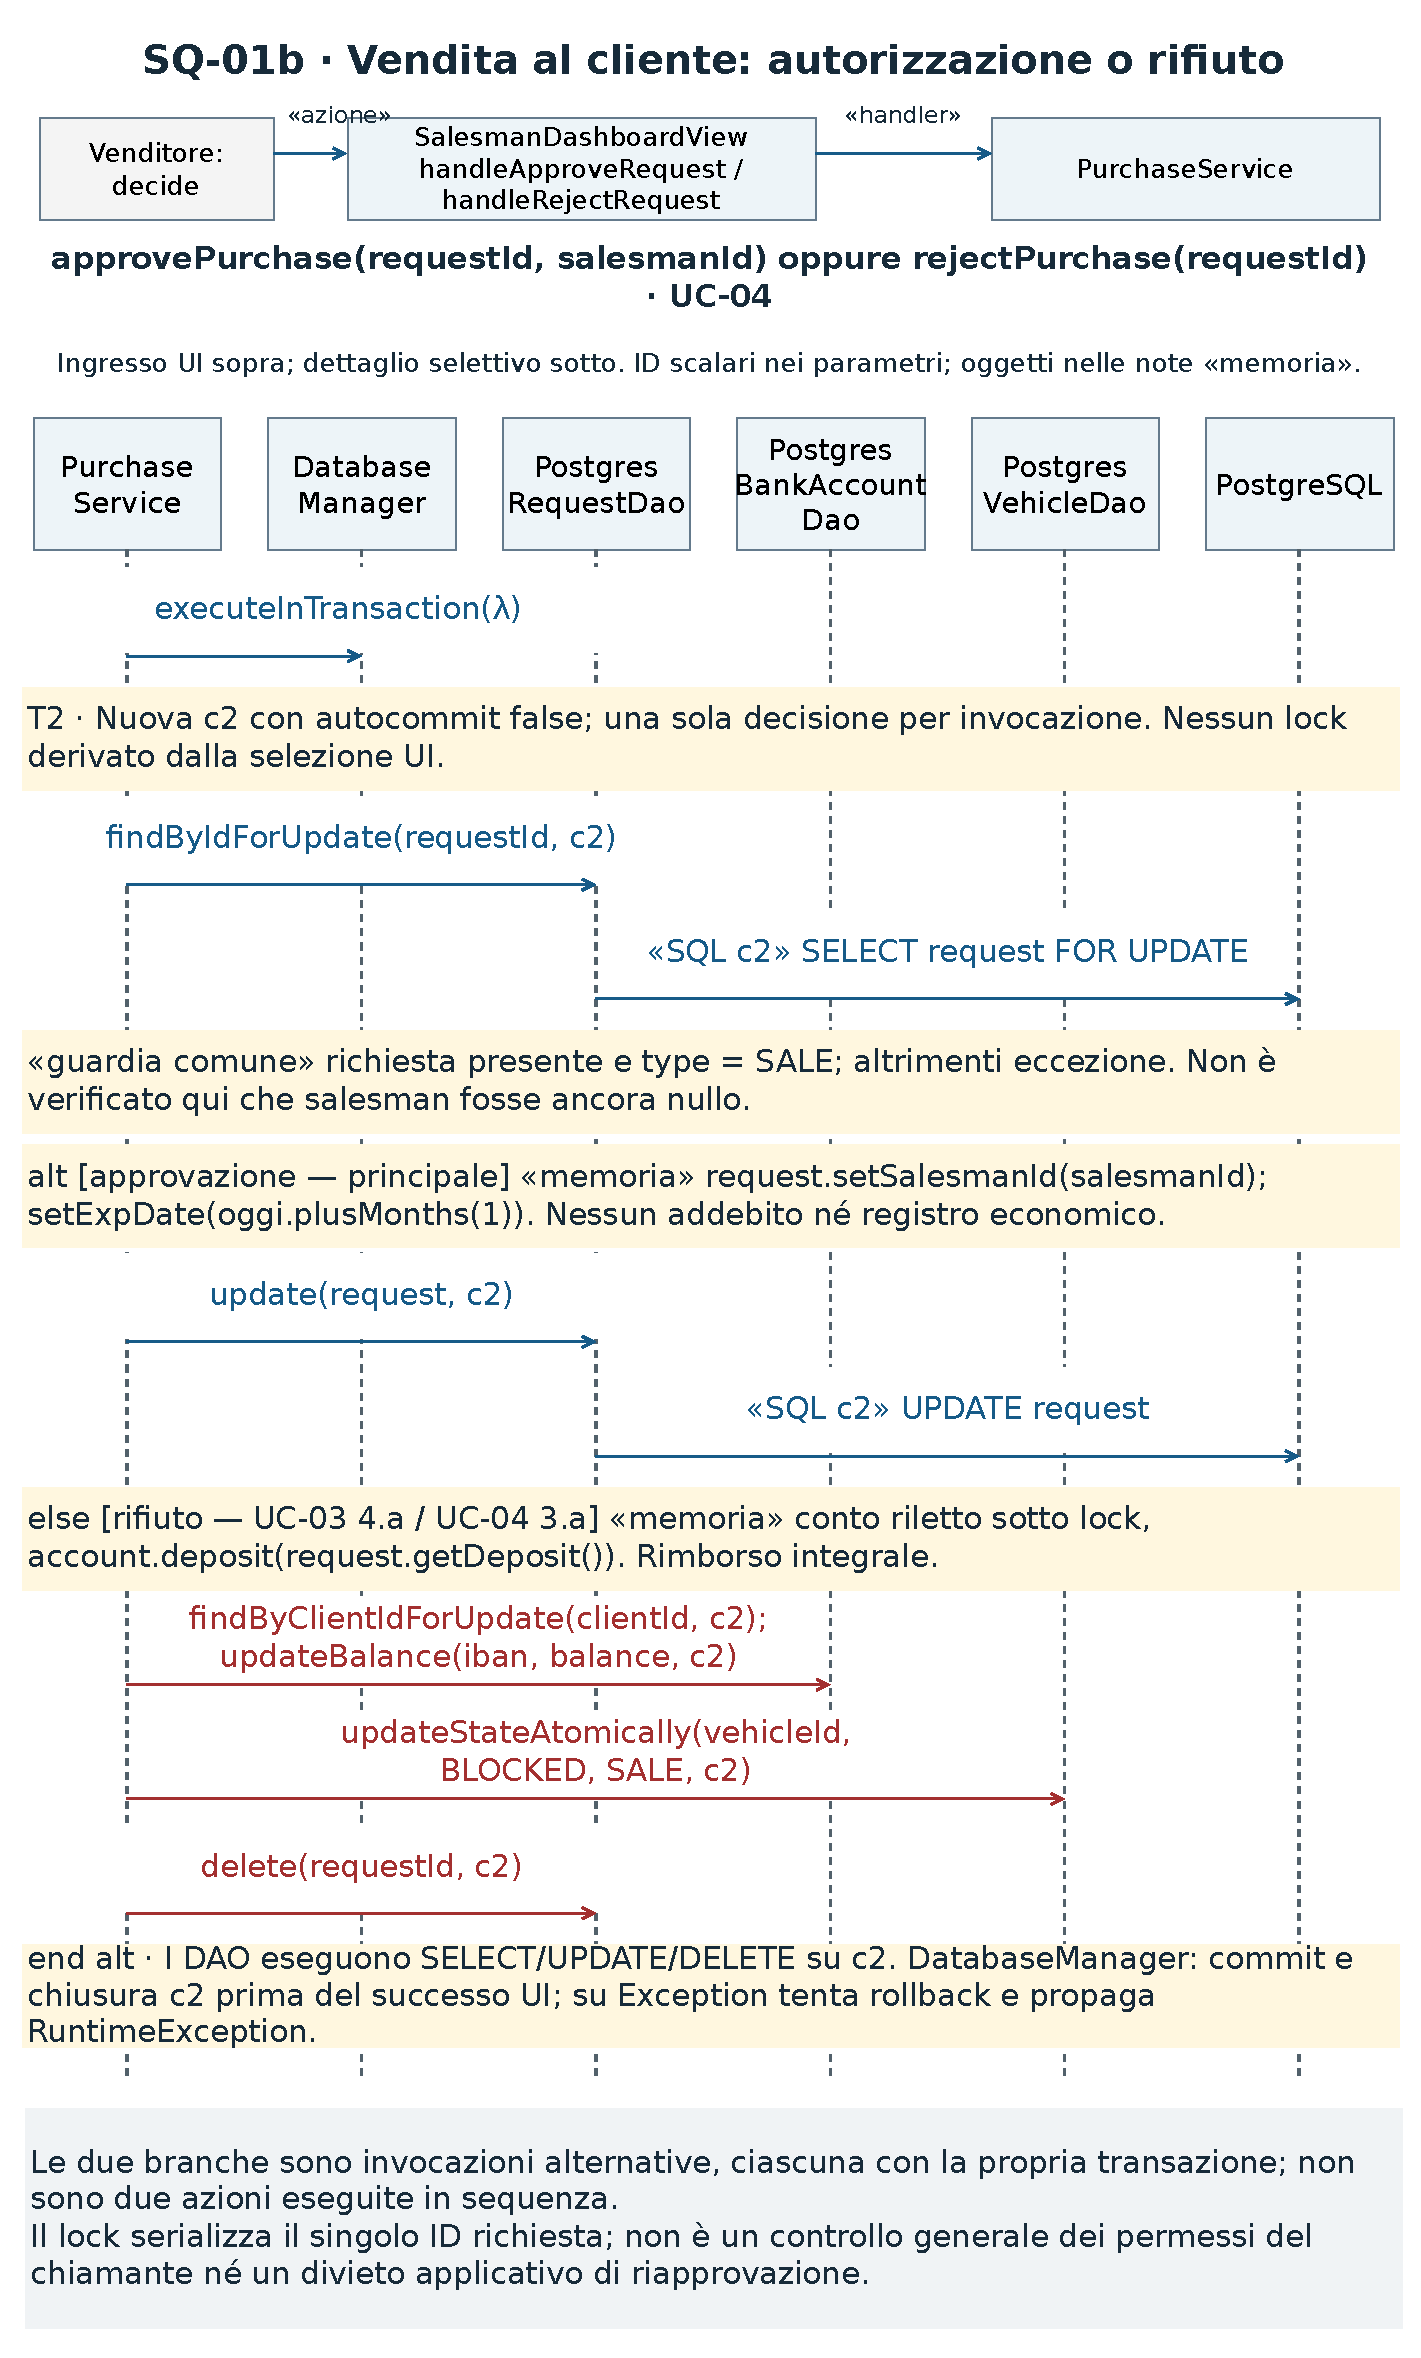
\includegraphics[width=\linewidth,height=.88\textheight,keepaspectratio]{diagrammi/sequenza-vendita-esito.drawio.pdf}
  \caption{SQ-01b --- UC-04: approvazione oppure rifiuto con rimborso.}\label{fig:sq01b}
\end{figure}
\begin{figure}[p]
  \centering
  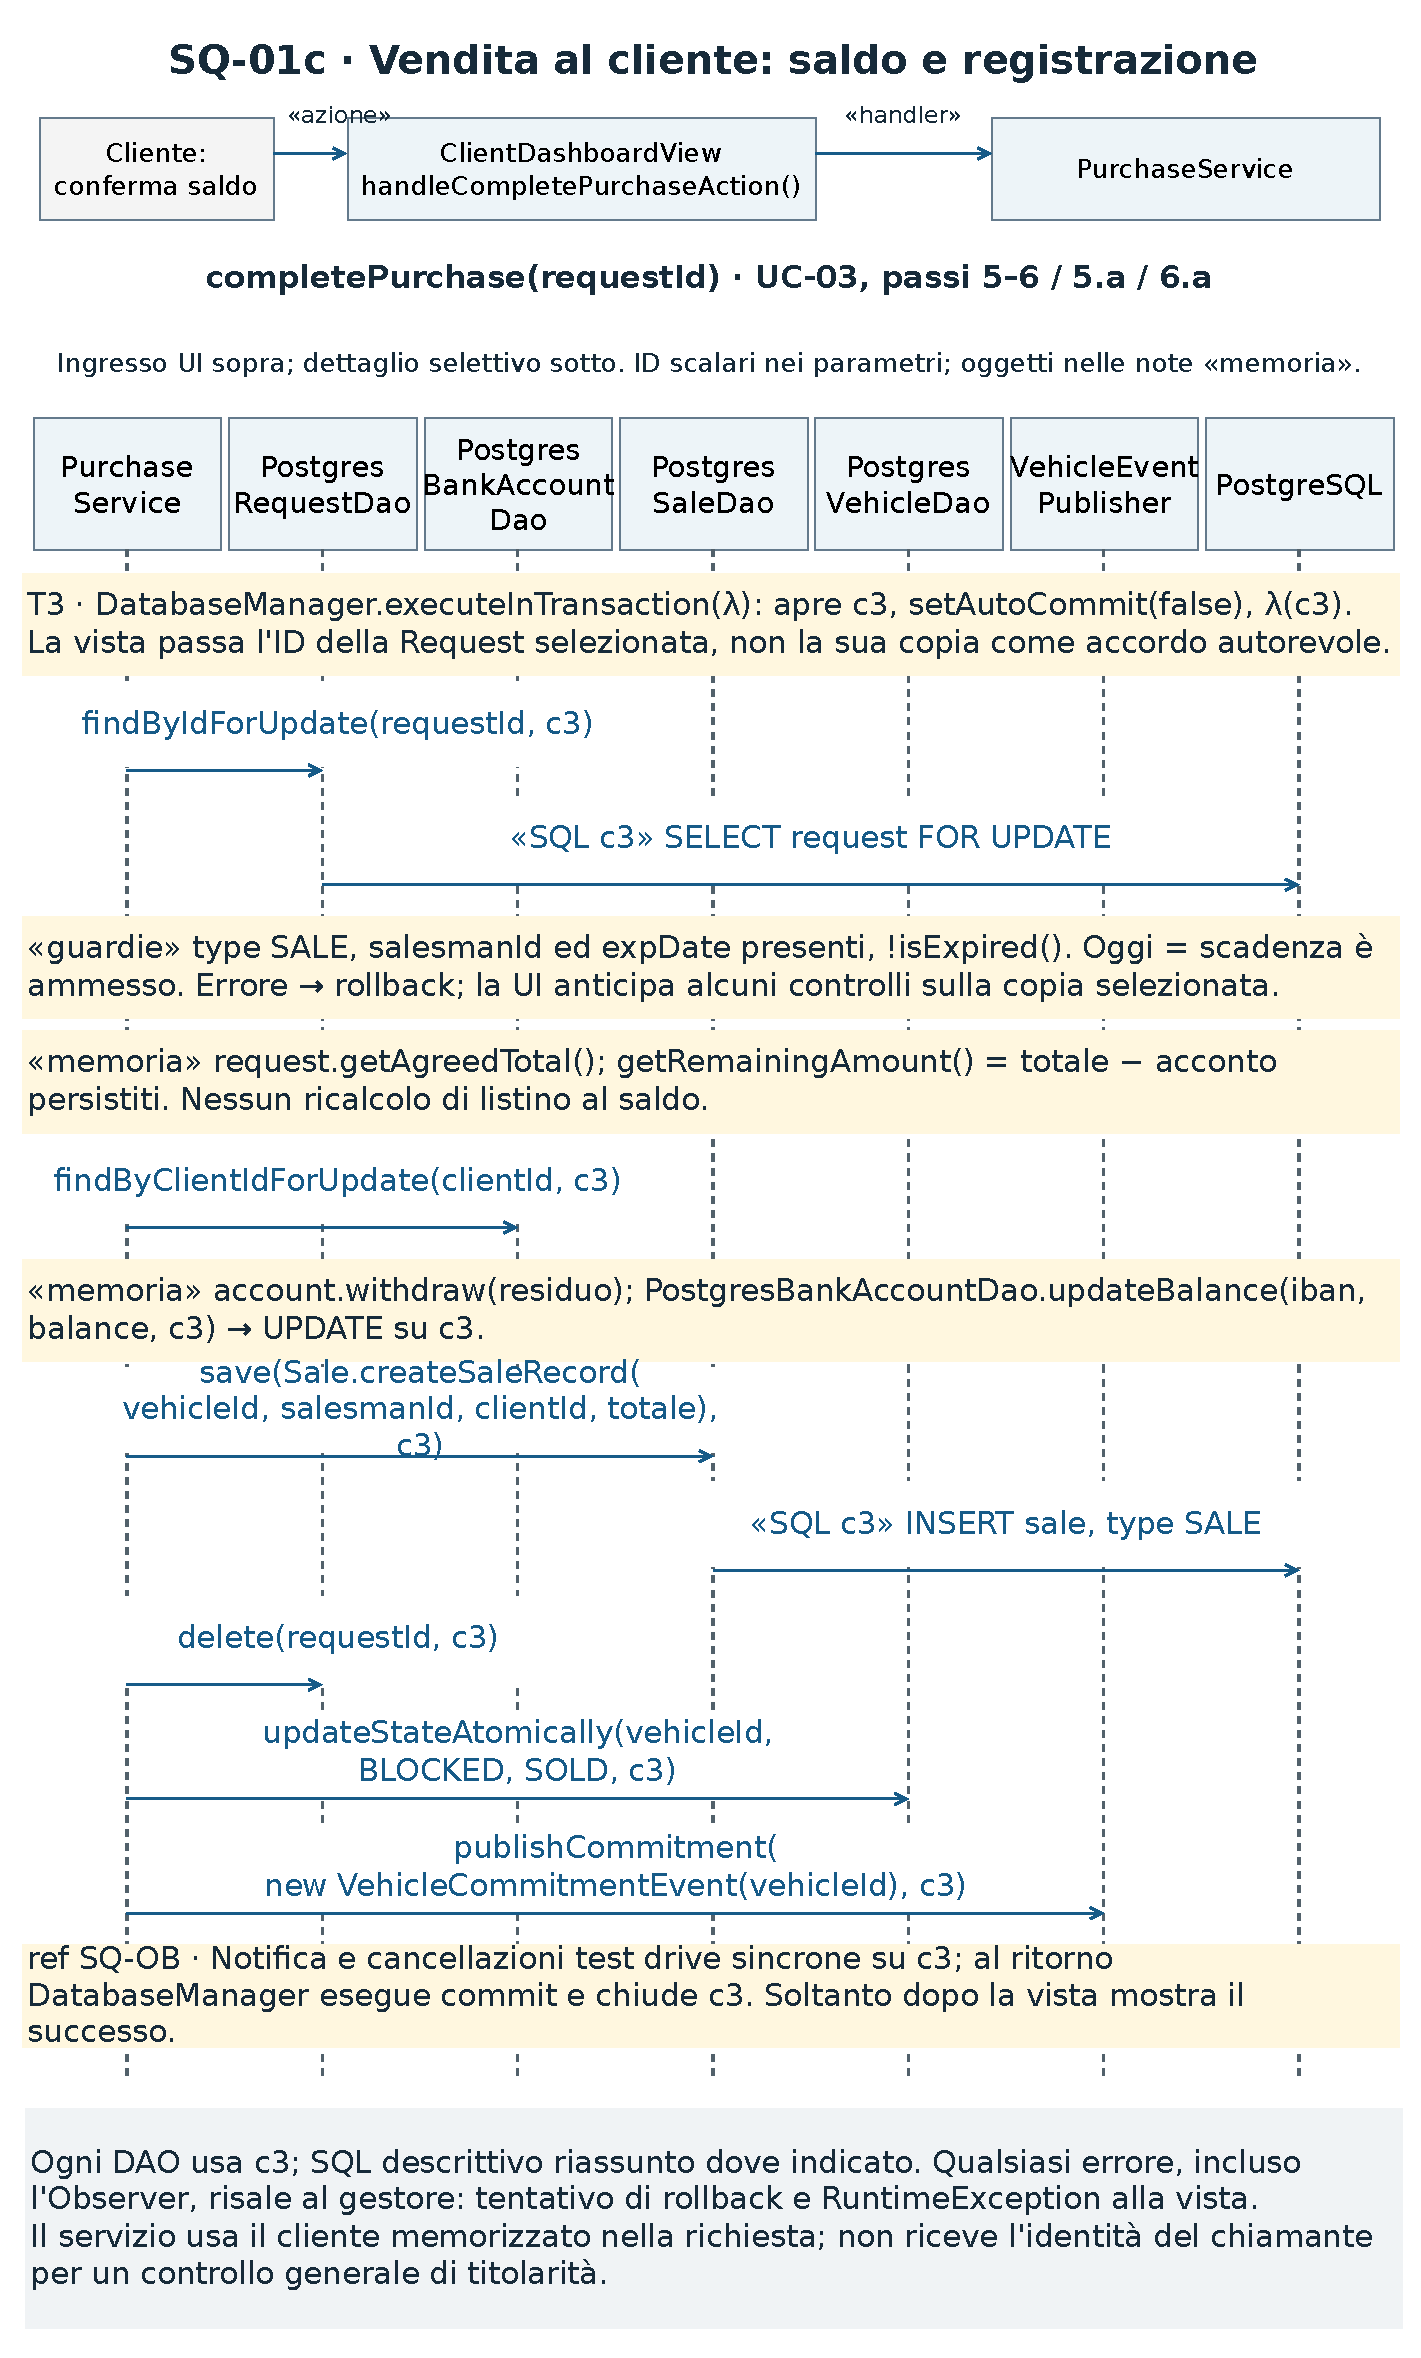
\includegraphics[width=\linewidth,height=.88\textheight,keepaspectratio]{diagrammi/sequenza-vendita-saldo.drawio.pdf}
  \caption{SQ-01c --- Saldo sul totale persistito e registrazione della vendita al cliente.}\label{fig:sq01c}
\end{figure}
\clearpage

SQ-01d (figura~\ref{fig:sq01d}) copre l'alternativa UC-03 6.b.
Il costruttore della dashboard cliente programma il controllo con
\code{Platform.runLater}: non è un processo periodico e il solo decorso
del tempo non esegue movimenti. Una lettura autonoma raccoglie i candidati;
ciascuno è poi riletto e valutato in una transazione propria. Per una
richiesta approvata con data strettamente precedente a oggi, il servizio
trattiene il 20\% dell'acconto, arrotondato ai centesimi, restituisce il resto,
registra \code{PENALTY}, elimina la richiesta e libera il veicolo.
La penale non è il 20\% del totale. Un candidato non più pertinente non
produce effetti; se un candidato fallisce, quelli già confermati restano
trattati. L'errore risale alla vista, che in questo controllo scrive un
avviso su stderr; i messaggi all'utente sono mostrati solo al ritorno
normale della lista. Non si produce una notifica Observer.

\begin{figure}[p]
  \centering
  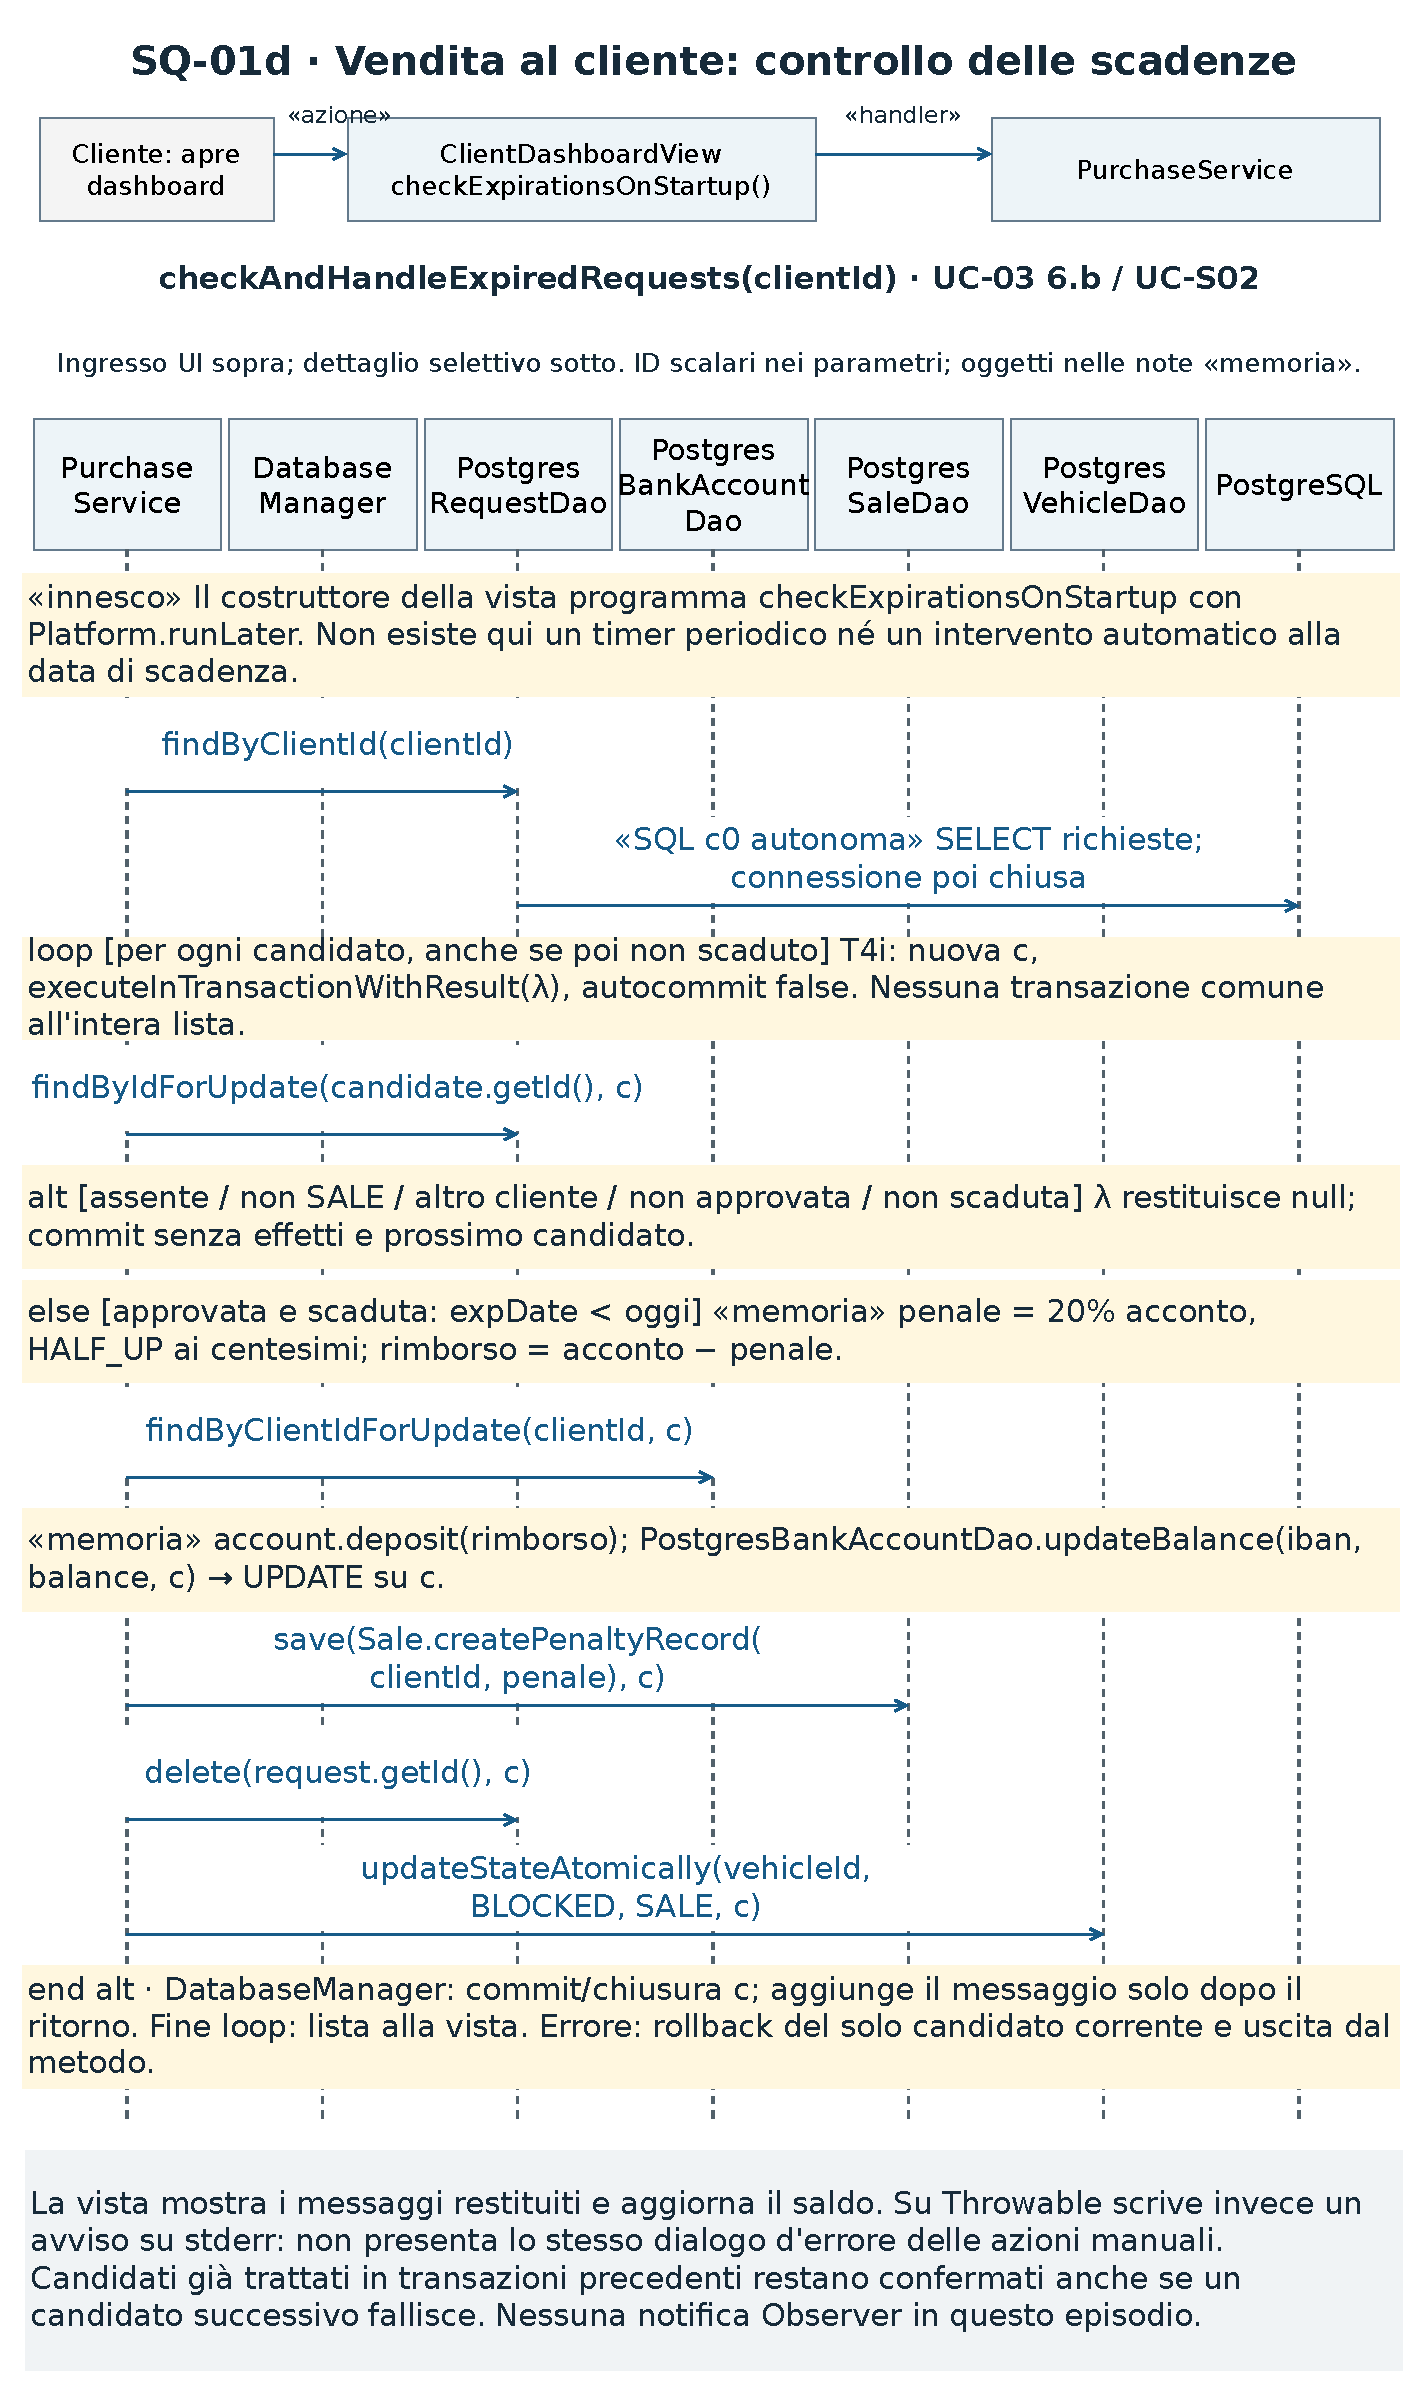
\includegraphics[width=\linewidth,height=.88\textheight,keepaspectratio]{diagrammi/sequenza-vendita-scadenza.drawio.pdf}
  \caption{SQ-01d --- Scadenze controllate all'apertura della dashboard, una transazione per candidato.}\label{fig:sq01d}
\end{figure}
\clearpage

\subsection{Prenotazione di un noleggio}
La tavola d'insieme riprende il flusso originale con i collaboratori attuali;
le viste successive approfondiscono transazioni e alternative.
\tavolaautori{sequenza-noleggio-insieme}{Noleggio: prenotazione e impegno commerciale}{fig:sq-noleggio-insieme}
\clearpage

SQ-02 (figura~\ref{fig:sq02}) realizza UC-02. Il preventivo del dialogo
è calcolato in una chiamata distinta e non congela un accordo.
Alla conferma, il servizio rifiuta date passate o invertite, blocca il
veicolo con \texttt{FOR UPDATE}, richiede \code{RENT} e blocca l'identità
cliente con \texttt{FOR NO KEY UPDATE}. Rilegge quindi la disponibilità sul
periodo incluso, ricalcola il costo e addebita il 100\% sotto lock del conto.
Gli overload PostgreSQL delle letture di modello e sconti usati qui
ricevono la stessa connessione: ciò non equivale a uno snapshot globale
immutabile né a un lock dell'intero listino. Lo stato rimane \code{RENT}.

Il controllo applicativo dei periodi è affiancato dal vincolo SQL
\code{EXCLUDE} sui noleggi dello stesso veicolo. Dopo il salvataggio,
la collaborazione SQ-OB (figura~\ref{fig:sqob}) cancella \emph{tutti} i
test drive futuri del veicolo, anche esterni al periodo noleggiato:
è la priorità commerciale condivisa con il saldo della vendita al cliente.
Il publisher chiama direttamente l'Observer sullo stesso thread e sulla
stessa connessione, prima del commit. Un errore della cancellazione risale
al gestore e impedisce di confermare addebito e prenotazione separatamente.
Non vi sono coda, outbox o consegna asincrona. Il servizio di noleggio
riespone le cause applicative riconosciute, mentre gli altri errori
rimangono avvolti; la vista presenta il fallimento. Non si estende questa
garanzia ad altre operazioni o a qualsiasi protocollo concorrente.

\begin{figure}[p]
  \centering
  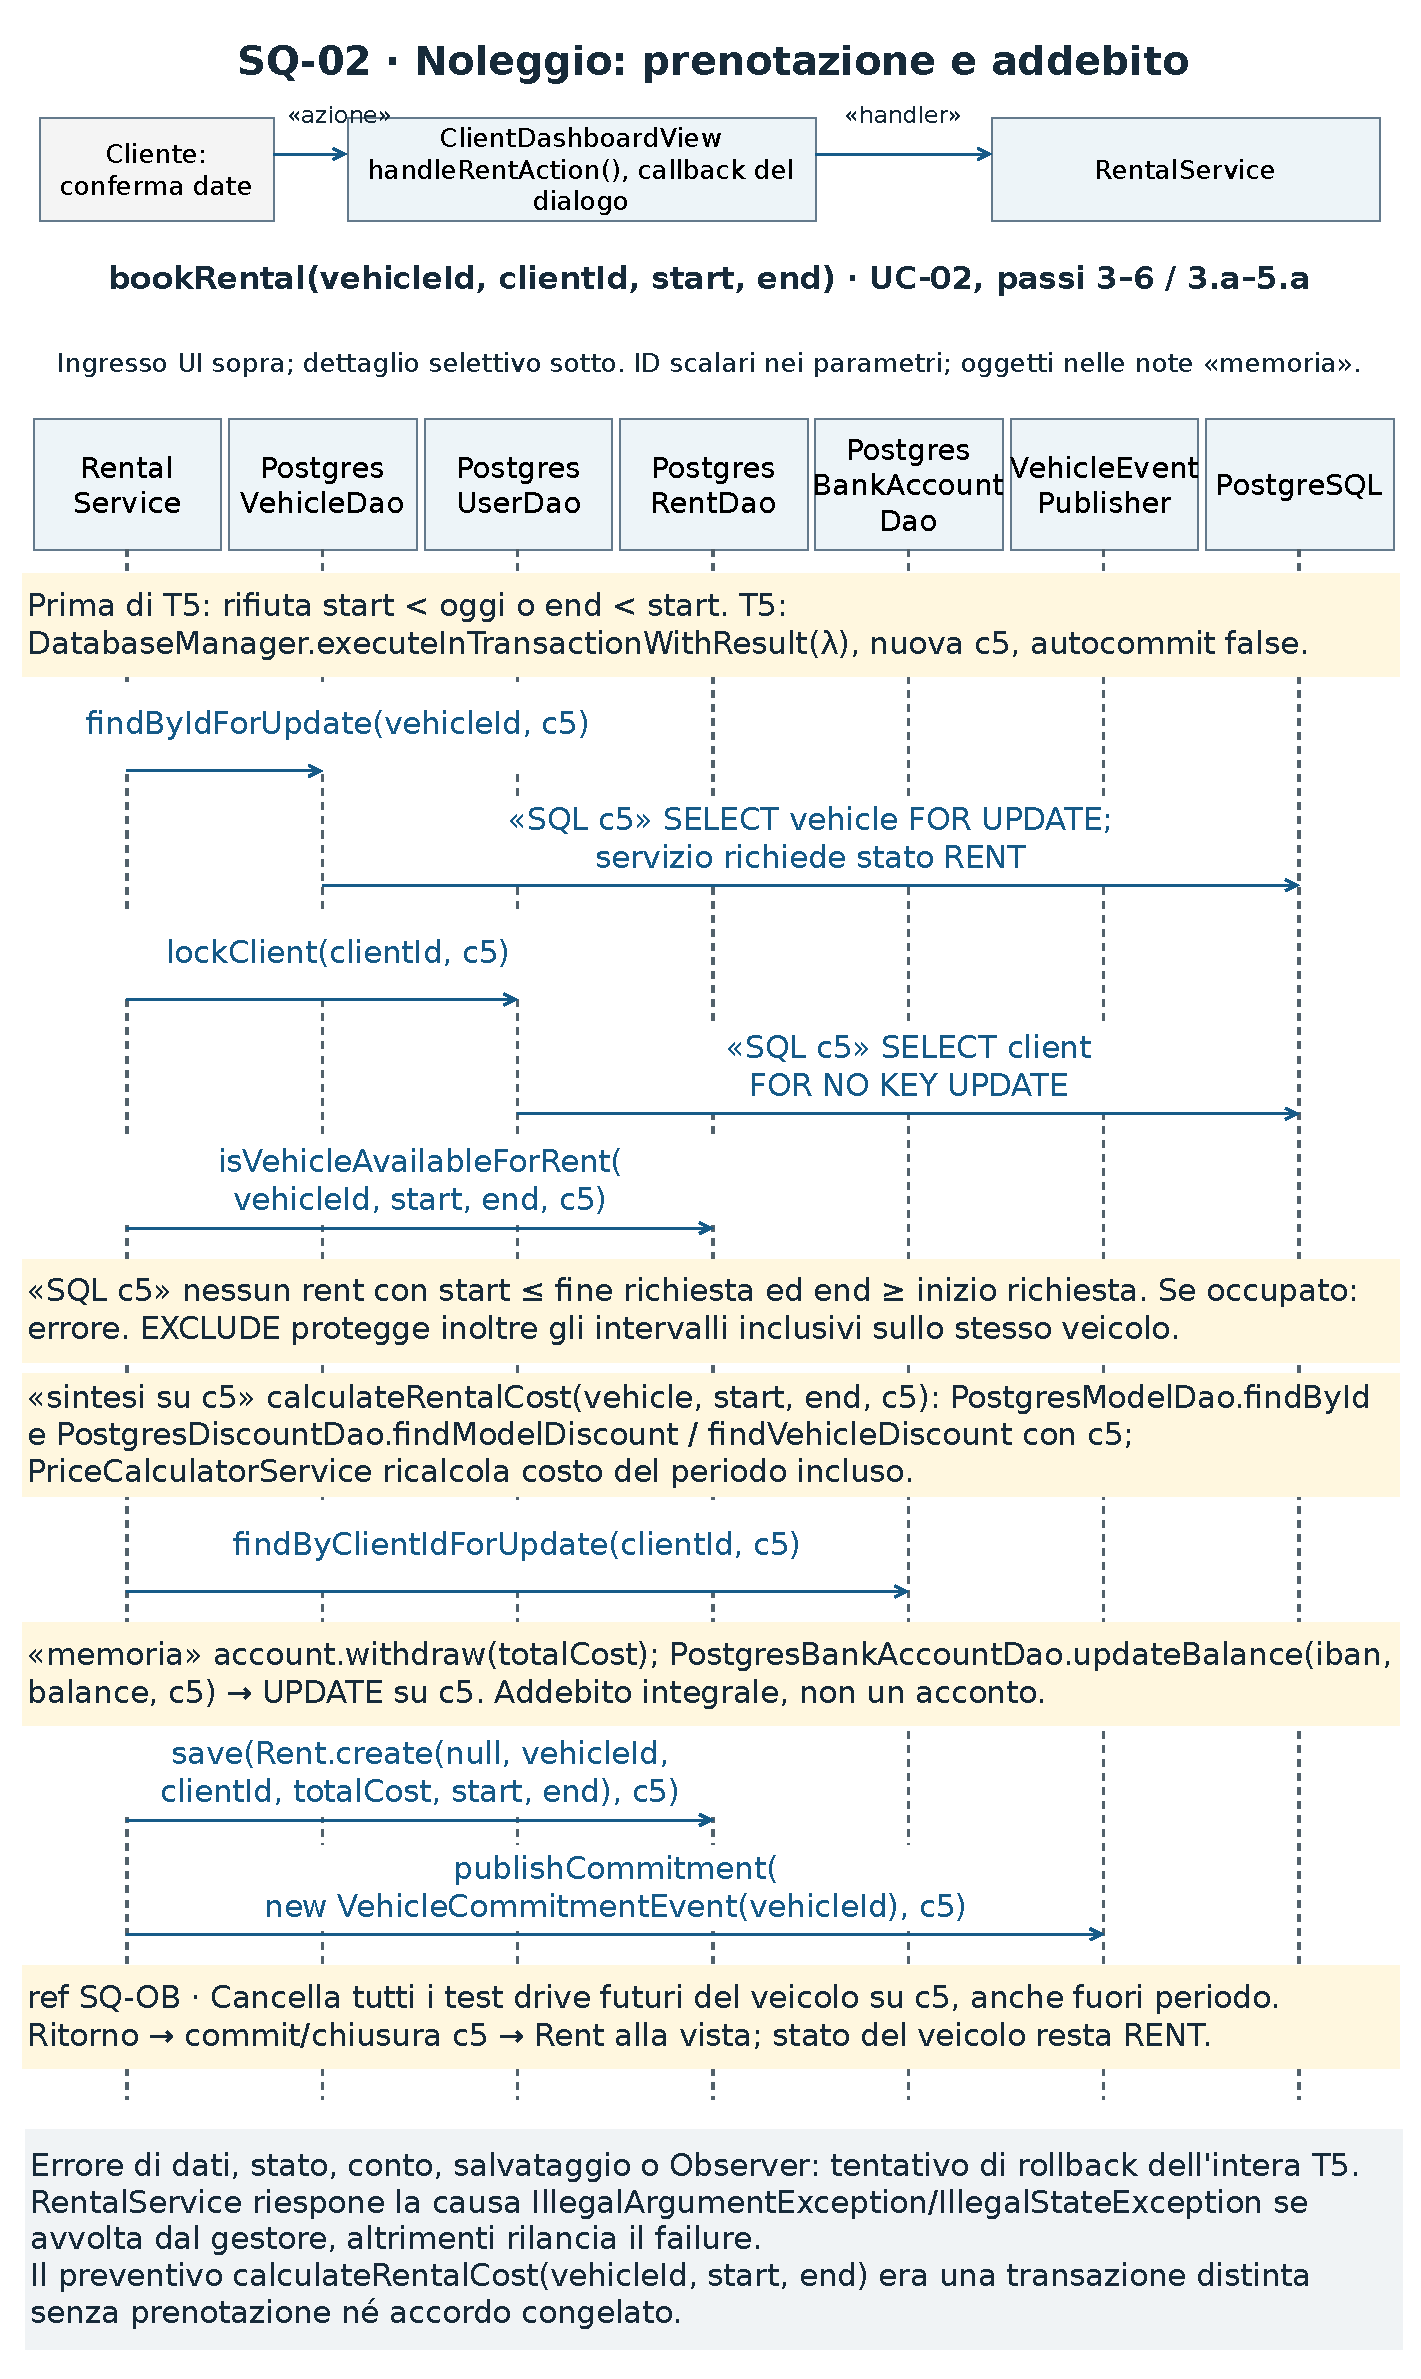
\includegraphics[width=\linewidth,height=.88\textheight,keepaspectratio]{diagrammi/sequenza-noleggio.drawio.pdf}
  \caption{SQ-02 --- Noleggio: disponibilità, costo ricalcolato e addebito integrale.}\label{fig:sq02}
\end{figure}
\begin{figure}[p]
  \centering
  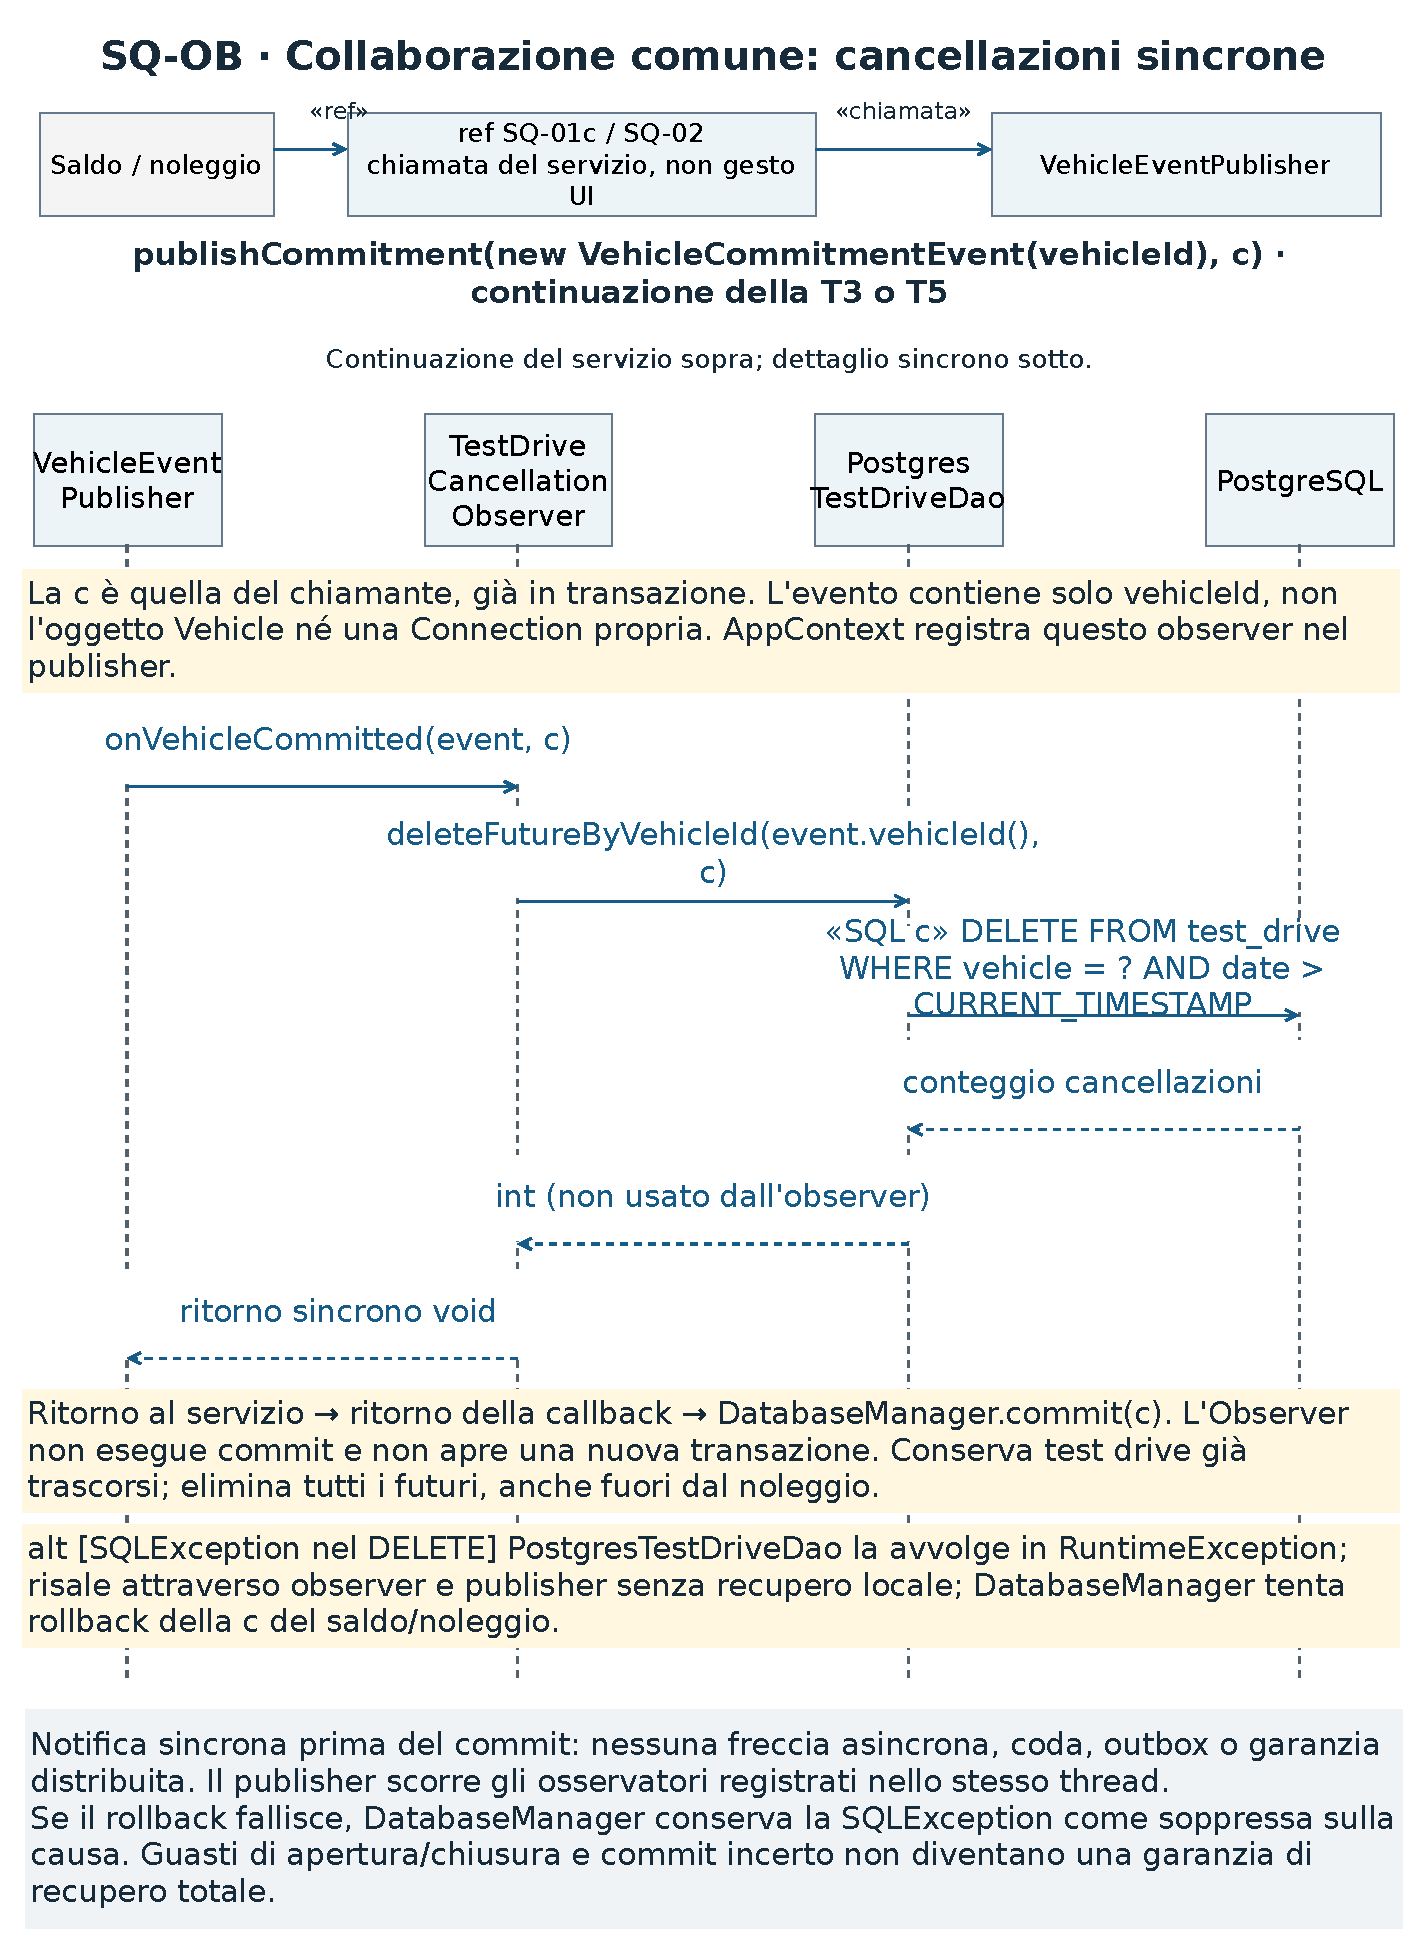
\includegraphics[width=\linewidth,height=.88\textheight,keepaspectratio]{diagrammi/sequenza-observer.drawio.pdf}
  \caption{SQ-OB --- Cancellazioni Observer condivise da SQ-01c e SQ-02, sincrone sulla connessione del chiamante.}\label{fig:sqob}
\end{figure}
\clearpage

\subsection{Acquisto di un veicolo dal cliente}
La tavola d'insieme riprende il flusso originale con i collaboratori attuali;
le viste successive approfondiscono transazioni e alternative.
\tavolaautori{sequenza-cessione-insieme}{Acquisto dal cliente: proposta ed esito}{fig:sq-cessione-insieme}
\clearpage

L'acquisto dal cliente di UC-05 ha due episodi distinti.
SQ-03a (figura~\ref{fig:sq03a}) registra la proposta e non effettua
pagamenti. Se il VIN è noto, il veicolo deve essere \code{SOLD},
l'ultima vendita al cliente deve attribuirlo al proponente e non devono
esistere richieste aperte; modello e anno devono coincidere. Il lock
\texttt{FOR UPDATE} riguarda una riga esistente, non un VIN assente.
Per un VIN nuovo viene creato il veicolo; in entrambi i casi lo stato
è \code{WAITING}. Il servizio ricalcola la stima e la salva in
\code{Request.deposit}, di tipo \code{PURCHASE}, con
\code{agreed\_total} nullo. Le letture autonome del modello e dello
sconto modello non appartengono a T6. La stima persistita, non il
preventivo facoltativo della UI, fissa l'importo dell'eventuale accettazione.

SQ-03b (figura~\ref{fig:sq03b}) rilegge e blocca richiesta e veicolo,
richiedendo rispettivamente \code{PURCHASE} e \code{WAITING}.
L'accettazione richiede il venditore, accredita la stima memorizzata,
registra \code{Sale} di tipo \code{PURCHASE}, porta il veicolo a
\code{SALE} ed elimina la richiesta nella stessa transazione.
L'importo è non negativo ed esprime un esborso della concessionaria;
non è un acconto seguito da un saldo. Il rifiuto non movimenta il conto:
elimina la richiesta e, secondo le operazioni associate, ripristina
\code{SOLD} oppure elimina il veicolo senza storico. La presenza di
storico non sostituisce il controllo dell'ultima vendita al proponente.
Non interviene l'Observer. Un errore annulla l'esito corrente.

Un limite applicativo riguarda gli importi pari a zero: le richieste e
lo schema li ammettono, mentre il conto richiede movimenti strettamente
positivi. Un accredito o addebito zero nei percorsi rappresentati fallisce
e provoca rollback. Il limite del movimento non equivale quindi a un
divieto di conservare valori zero nelle richieste e nel registro.

\begin{figure}[p]
  \centering
  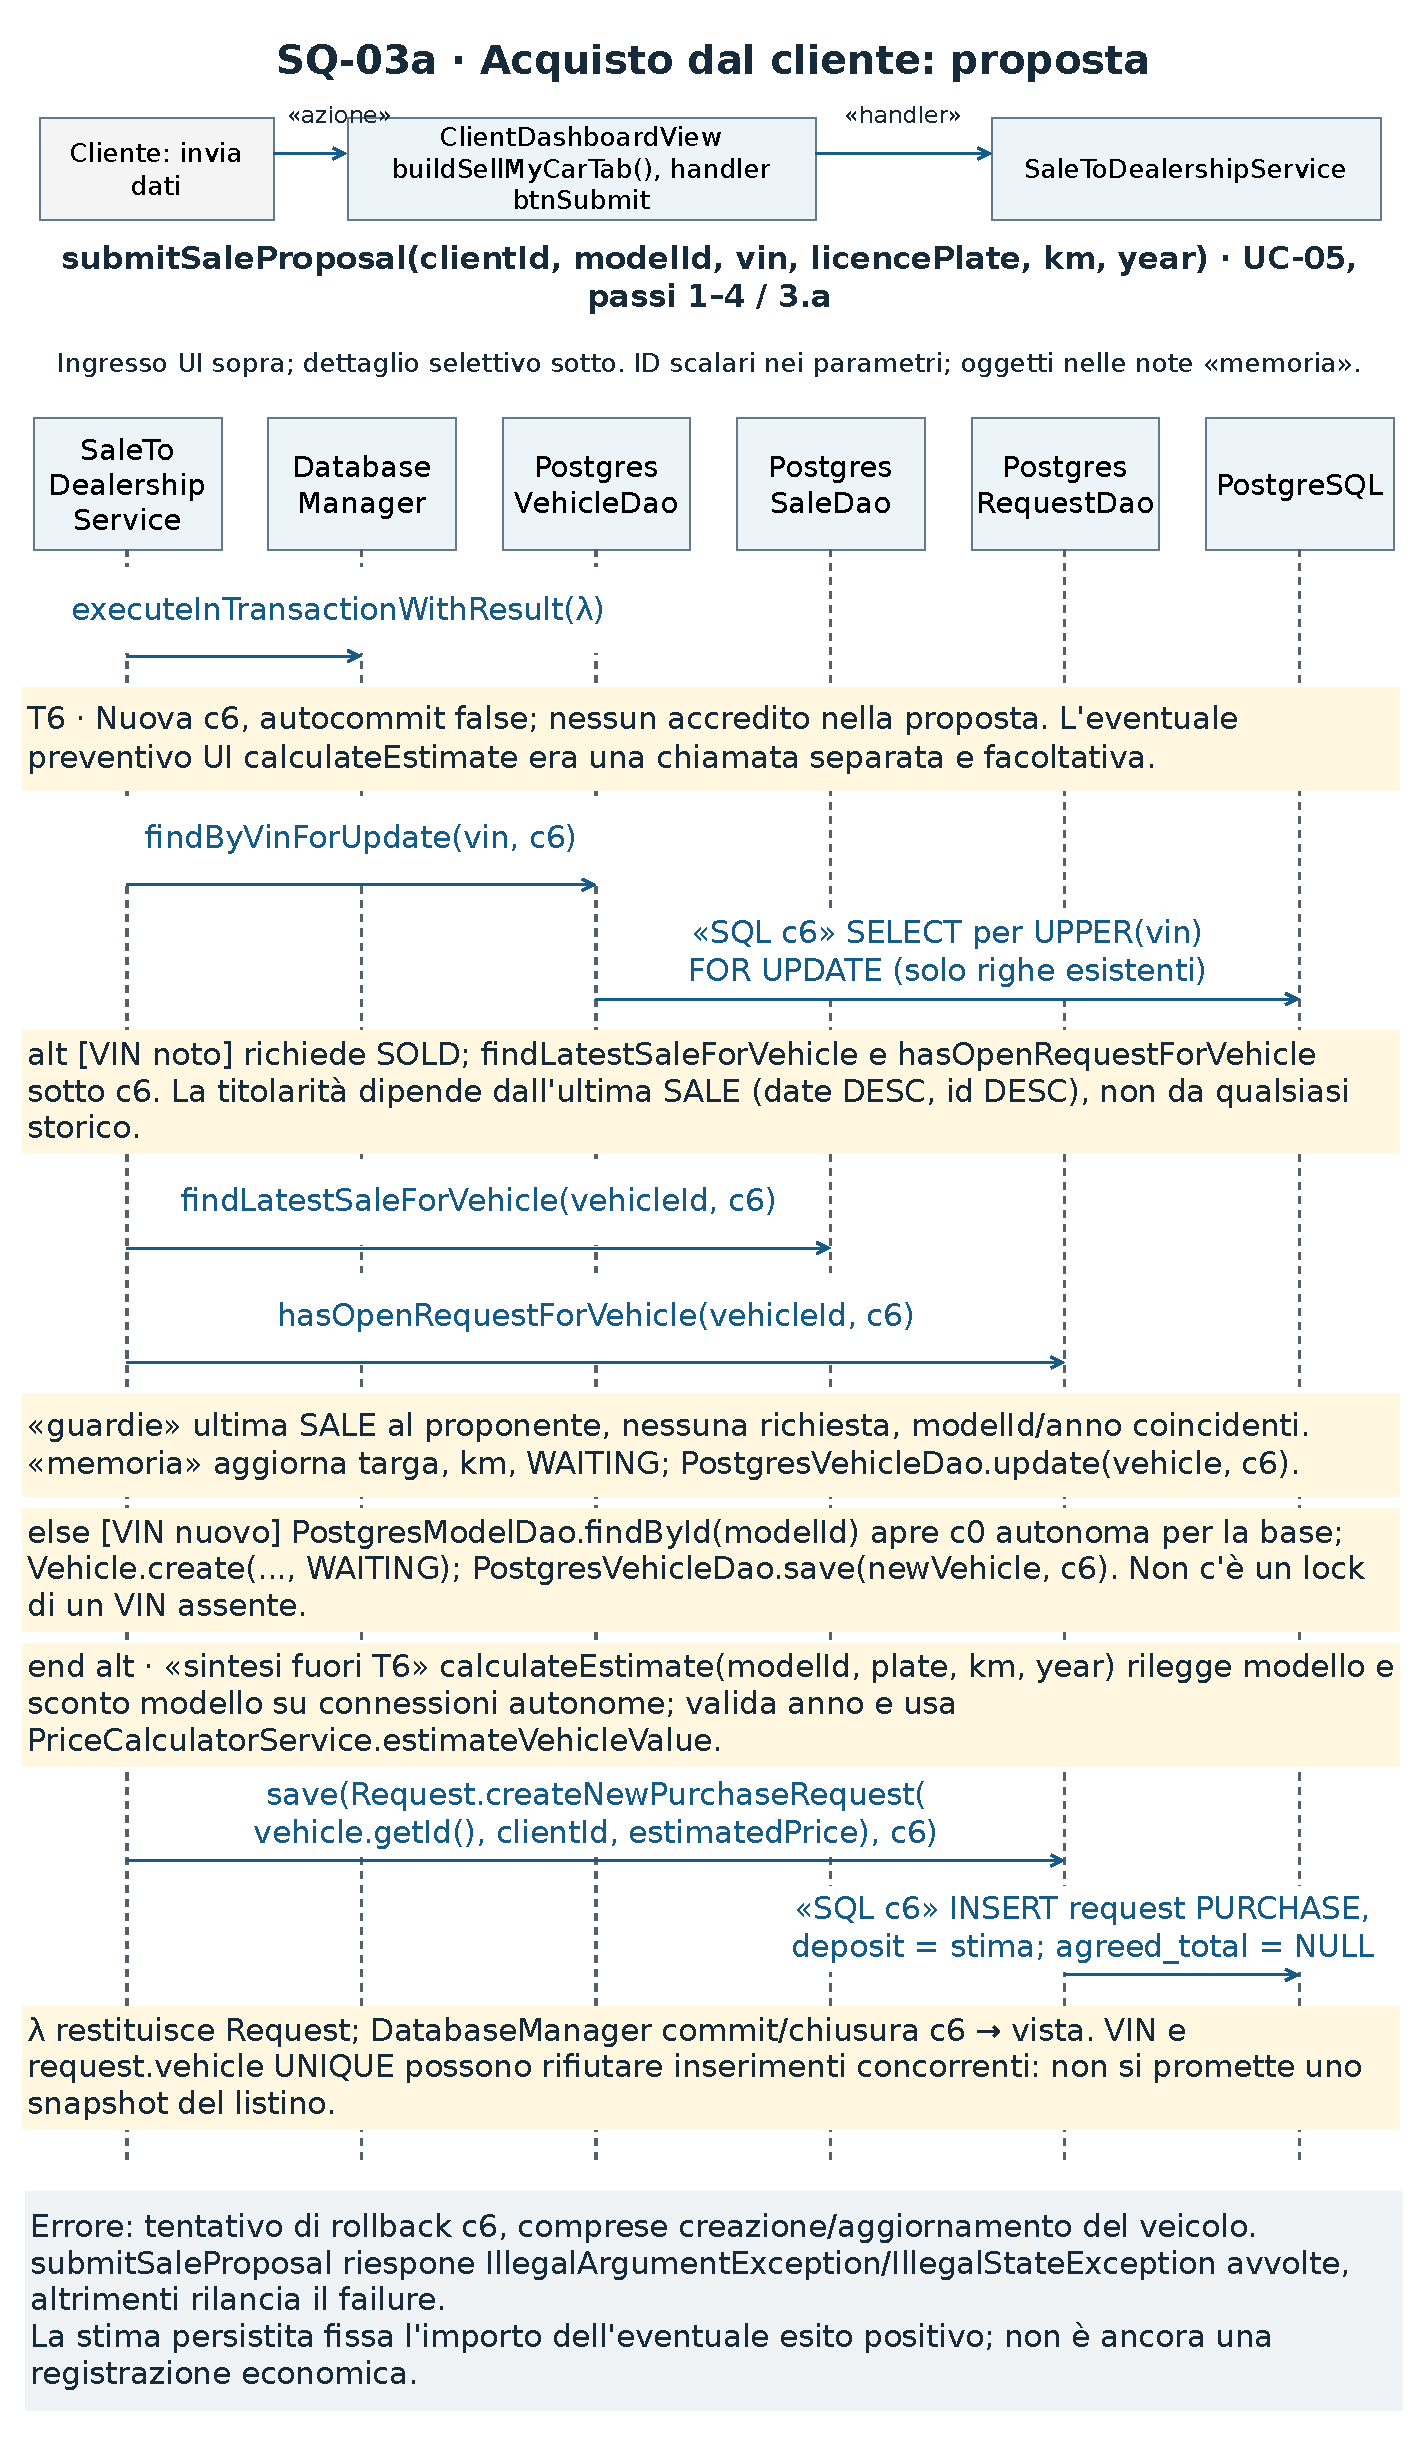
\includegraphics[width=\linewidth,height=.88\textheight,keepaspectratio]{diagrammi/sequenza-cessione-proposta.drawio.pdf}
  \caption{SQ-03a --- Proposta di cessione: veicolo in attesa e stima persistita, senza pagamento.}\label{fig:sq03a}
\end{figure}
\begin{figure}[p]
  \centering
  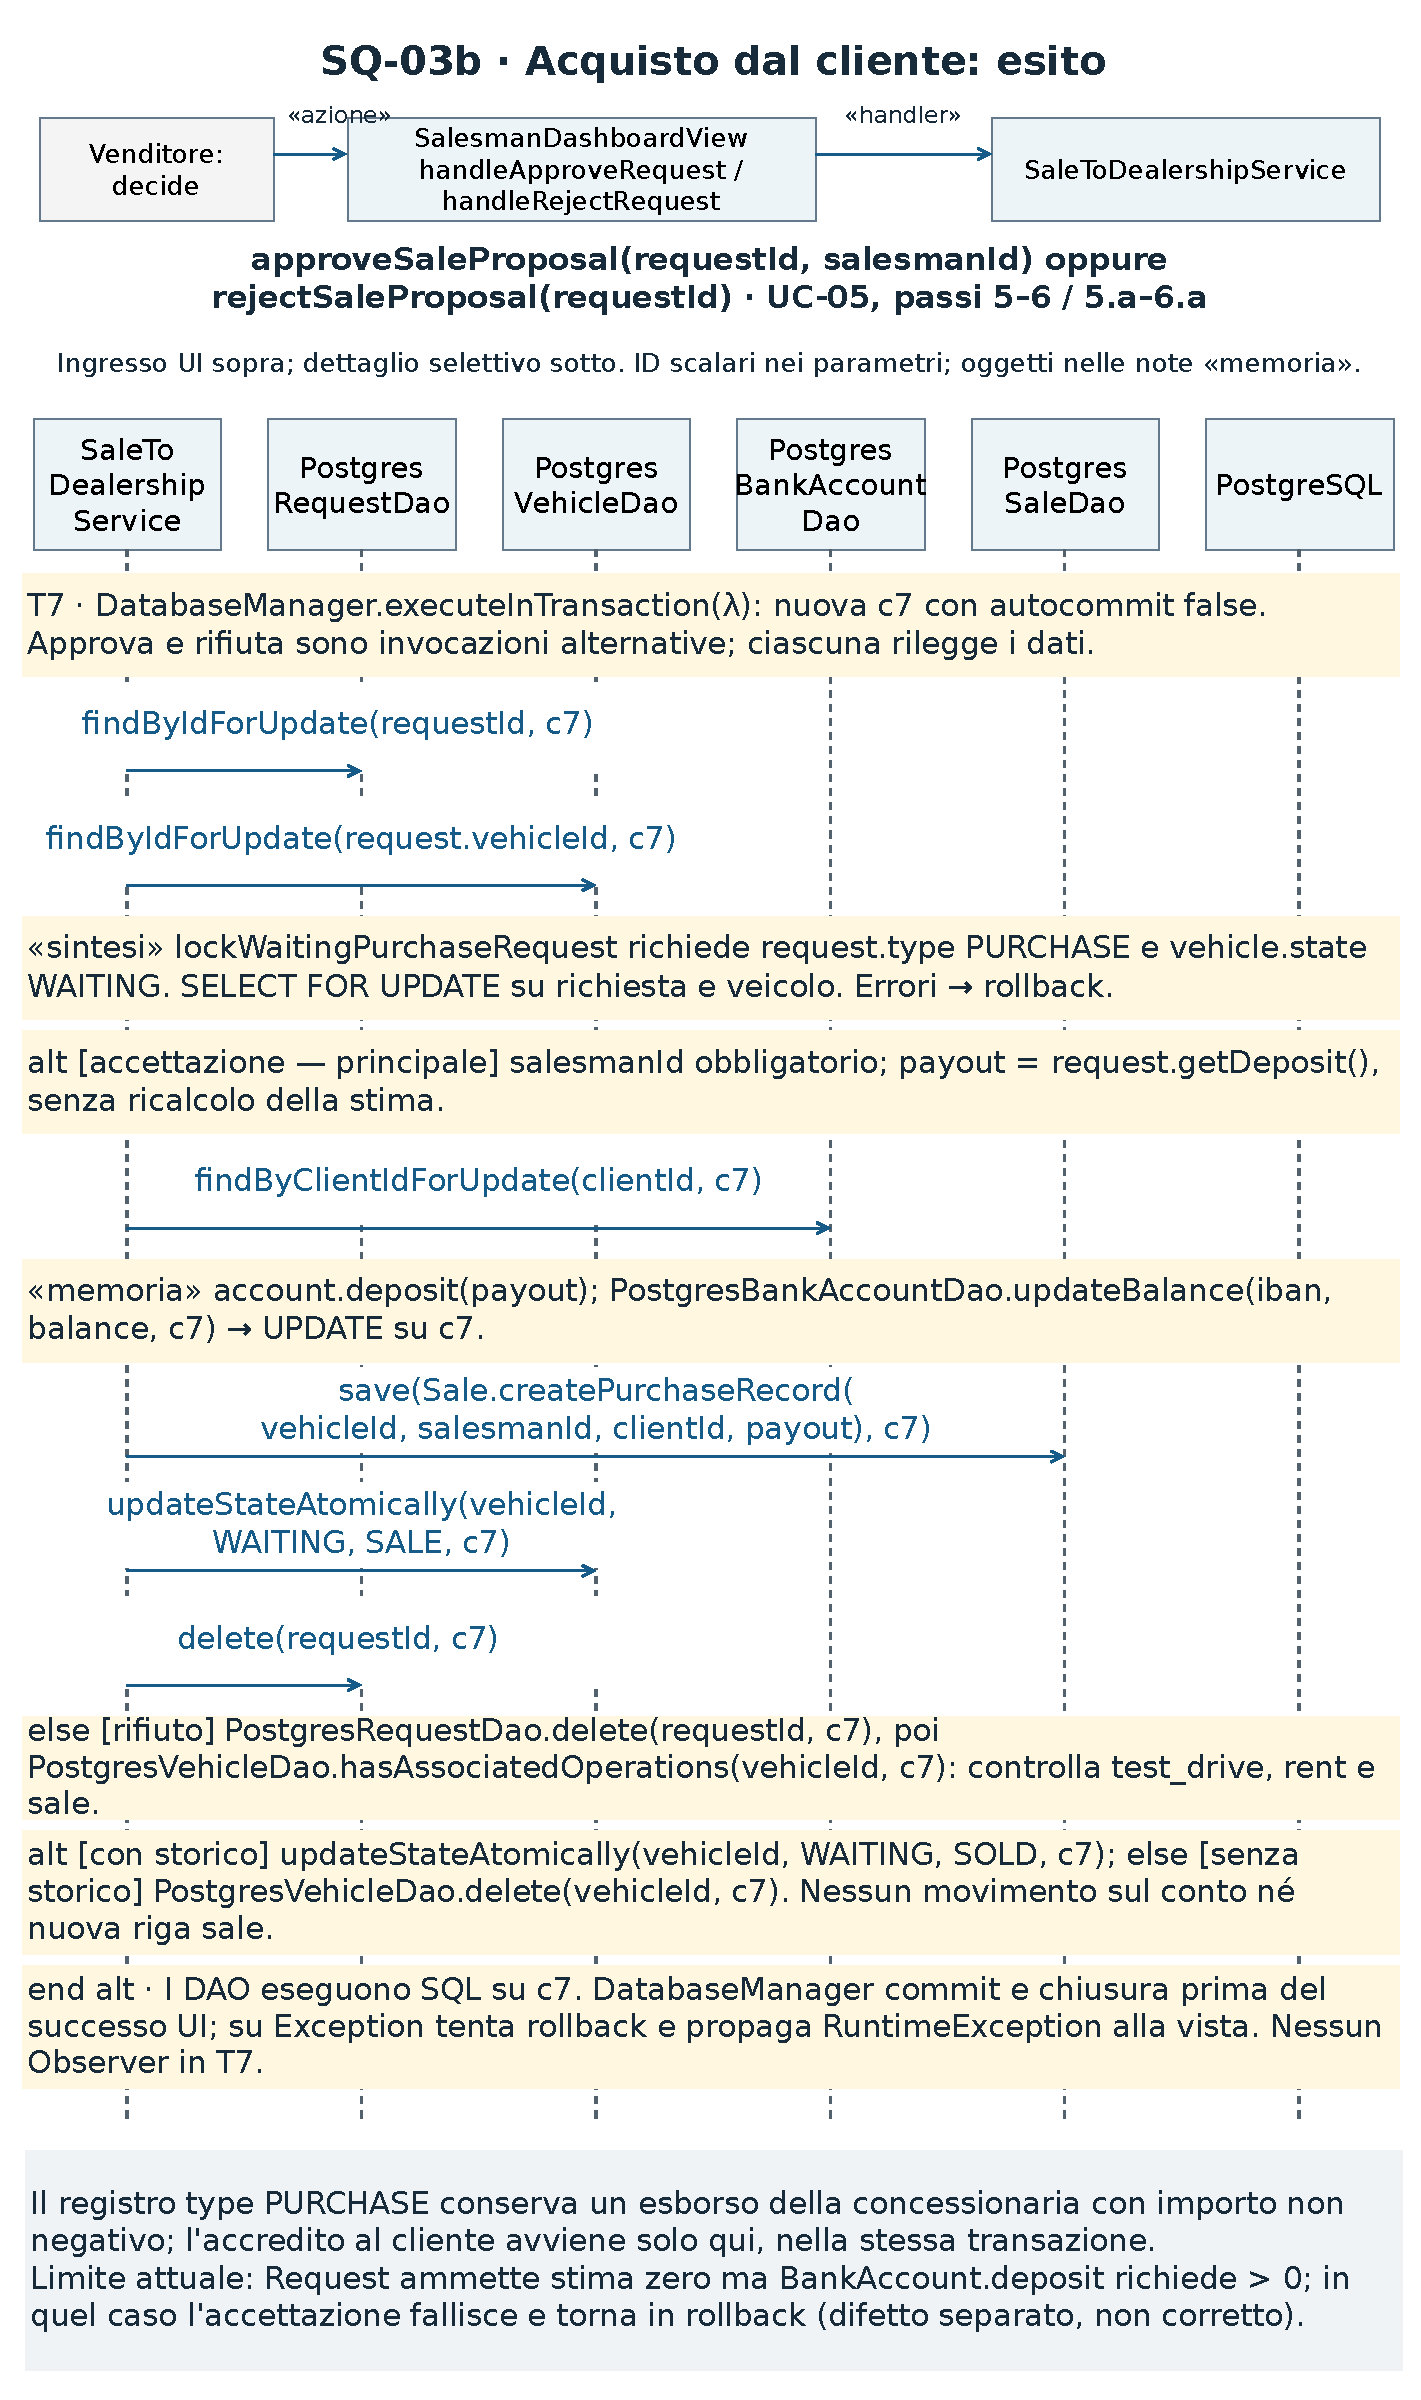
\includegraphics[width=\linewidth,height=.88\textheight,keepaspectratio]{diagrammi/sequenza-cessione-esito.drawio.pdf}
  \caption{SQ-03b --- Acquisto dal cliente: accettazione economica oppure rifiuto con conservazione dello storico.}\label{fig:sq03b}
\end{figure}
\clearpage

\section{Database}\label{sec:database}
Il modello descrive il DDL PostgreSQL corrente di \code{schema.sql},
riscontrato con mapping DAO e dominio: comprende tredici tabelle,
quindici chiavi esterne, una vista delle identità e una sequenza comune
agli utenti applicativi. Non è derivato dalle classi Java né ottenuto
da un'esportazione automatica. Le tavole distinguono il modello delle
relazioni dai controlli che richiedono la collaborazione dei servizi.

\subsection{Schema ER}
La figura~\ref{fig:er-autori} riprende \emph{SWE ER}, la tavola degli
autori, conservando tabelle a tre colonne, disposizione, generalizzazione
e cardinalit\`a a zampa di corvo. Sono aggiornati campi, tipi enumerati e
unicit\`a della richiesta per veicolo. Il nodo \emph{User} resta un
supertipo \textbf{concettuale}: non rappresenta una tabella padre, una PK
globale o un vincolo SQL di disgiunzione. Gli attributi comuni sono
ripetuti nelle tre tabelle di ruolo; PK e unicit\`a dell'email sono locali
a ciascuna. La seconda pagina conserva e corregge legenda e note.
Le due pagine A3 mantengono leggibile la tavola d'insieme; ER-01/02 e
REL-01--03 dettagliano poi relazioni, mapping e limiti dello schema.
\tavolaautori{database-er-autori}{Schema ER: tavola degli autori corretta, con notazione e gerarchia concettuale originali}{fig:er-autori}

Le viste ER-01 e ER-02 (figure~\ref{fig:er01} e~\ref{fig:er02}) sono
coordinate: i riquadri ripresi con lo stesso nome indicano la stessa
entità. Ogni arco dichiara entrambi i versi con minimo e massimo,
ricavati da nullabilità, unicità e FK, senza dedurli da riferimenti Java.
La parte catalogo collega marca, modello, veicolo e sconti. Ogni modello
ha una marca e ogni veicolo un modello; il padre può non avere figli.
Uno sconto appartiene a un solo modello o veicolo; la chiave condivisa
consente al padre zero o uno sconto.

Una richiesta riguarda esattamente un cliente e un veicolo; l'unicità
di \code{request.vehicle} limita a una la richiesta aperta per veicolo,
indipendentemente dal tipo. Il venditore è facoltativo. Test drive e
noleggio hanno entrambi cliente e veicolo obbligatori, con più operazioni
possibili nel tempo. Nel registro economico il cliente rimane obbligatorio,
mentre veicolo e venditore sono opzionali: il primo può anche essere
azzerato dalla cancellazione del veicolo. La penale prodotta dal servizio
non riferisce né veicolo né venditore; lo schema non impone questa
combinazione in funzione del tipo.

La vista ER delle identità mantiene le tre tabelle effettive, senza
inventare una tabella padre \code{user}. Il manager non è bersaglio di
FK applicative. Ogni conto appartiene a un cliente; \code{UNIQUE(client)}
consente a ciascun cliente al massimo un conto, ma nessuna FK impone
che ogni cliente ne possieda uno. La creazione congiunta è una scelta
transazionale di \code{AuthService}, non una partecipazione minima SQL.

\begin{figure}[p]
  \centering
  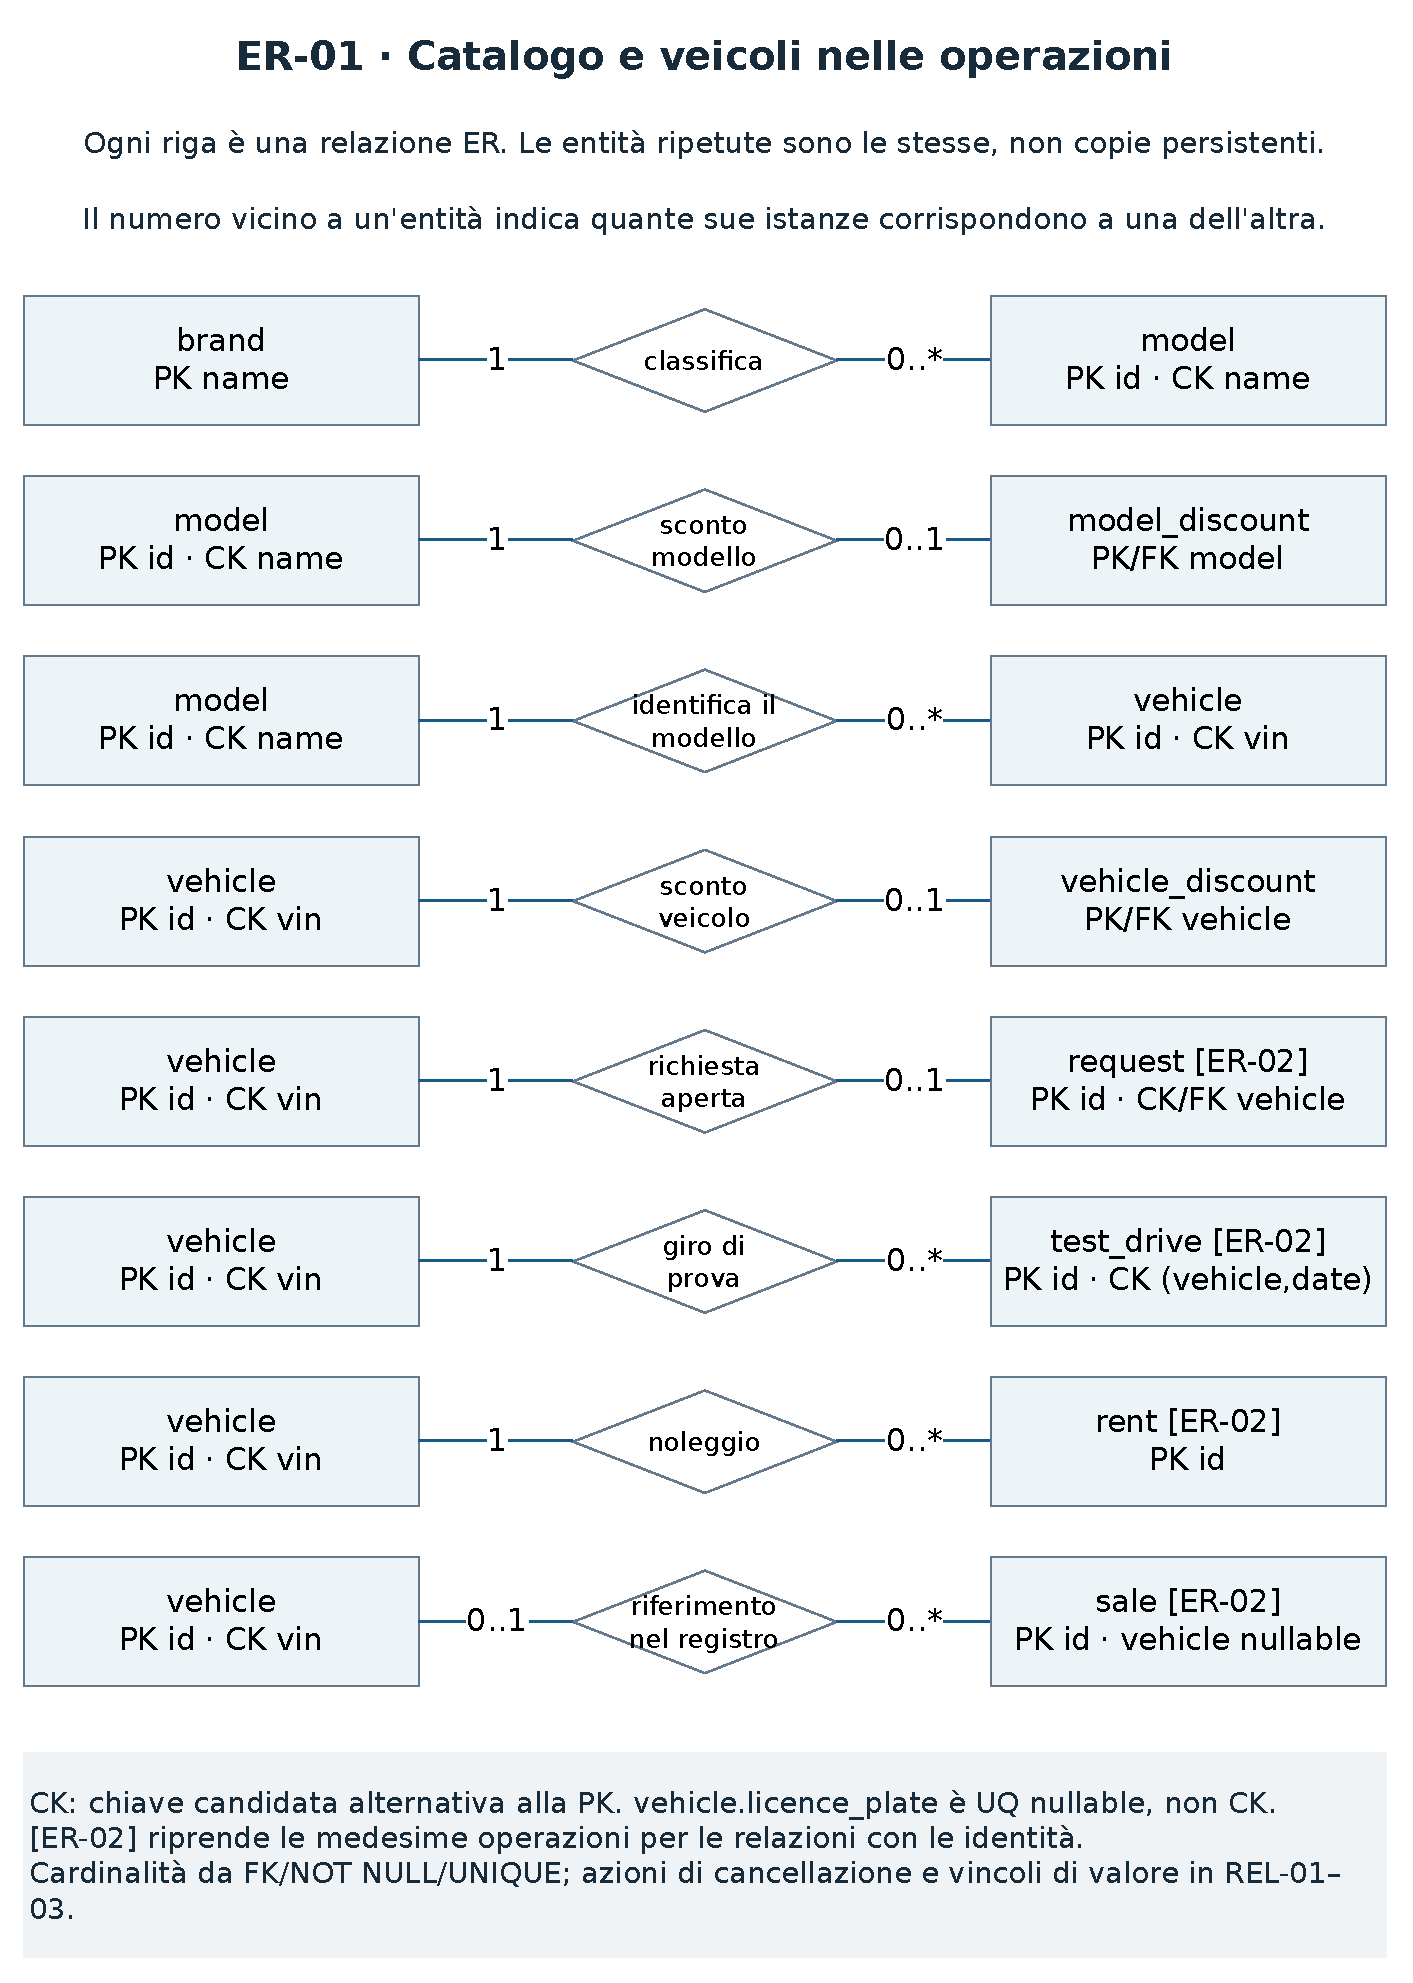
\includegraphics[width=\linewidth,height=.88\textheight,keepaspectratio]{diagrammi/database-er-catalogo.drawio.pdf}
  \caption{ER-01 --- Catalogo e riferimenti dei veicoli nelle operazioni; cardinalità nei due versi.}\label{fig:er01}
\end{figure}
\begin{figure}[p]
  \centering
  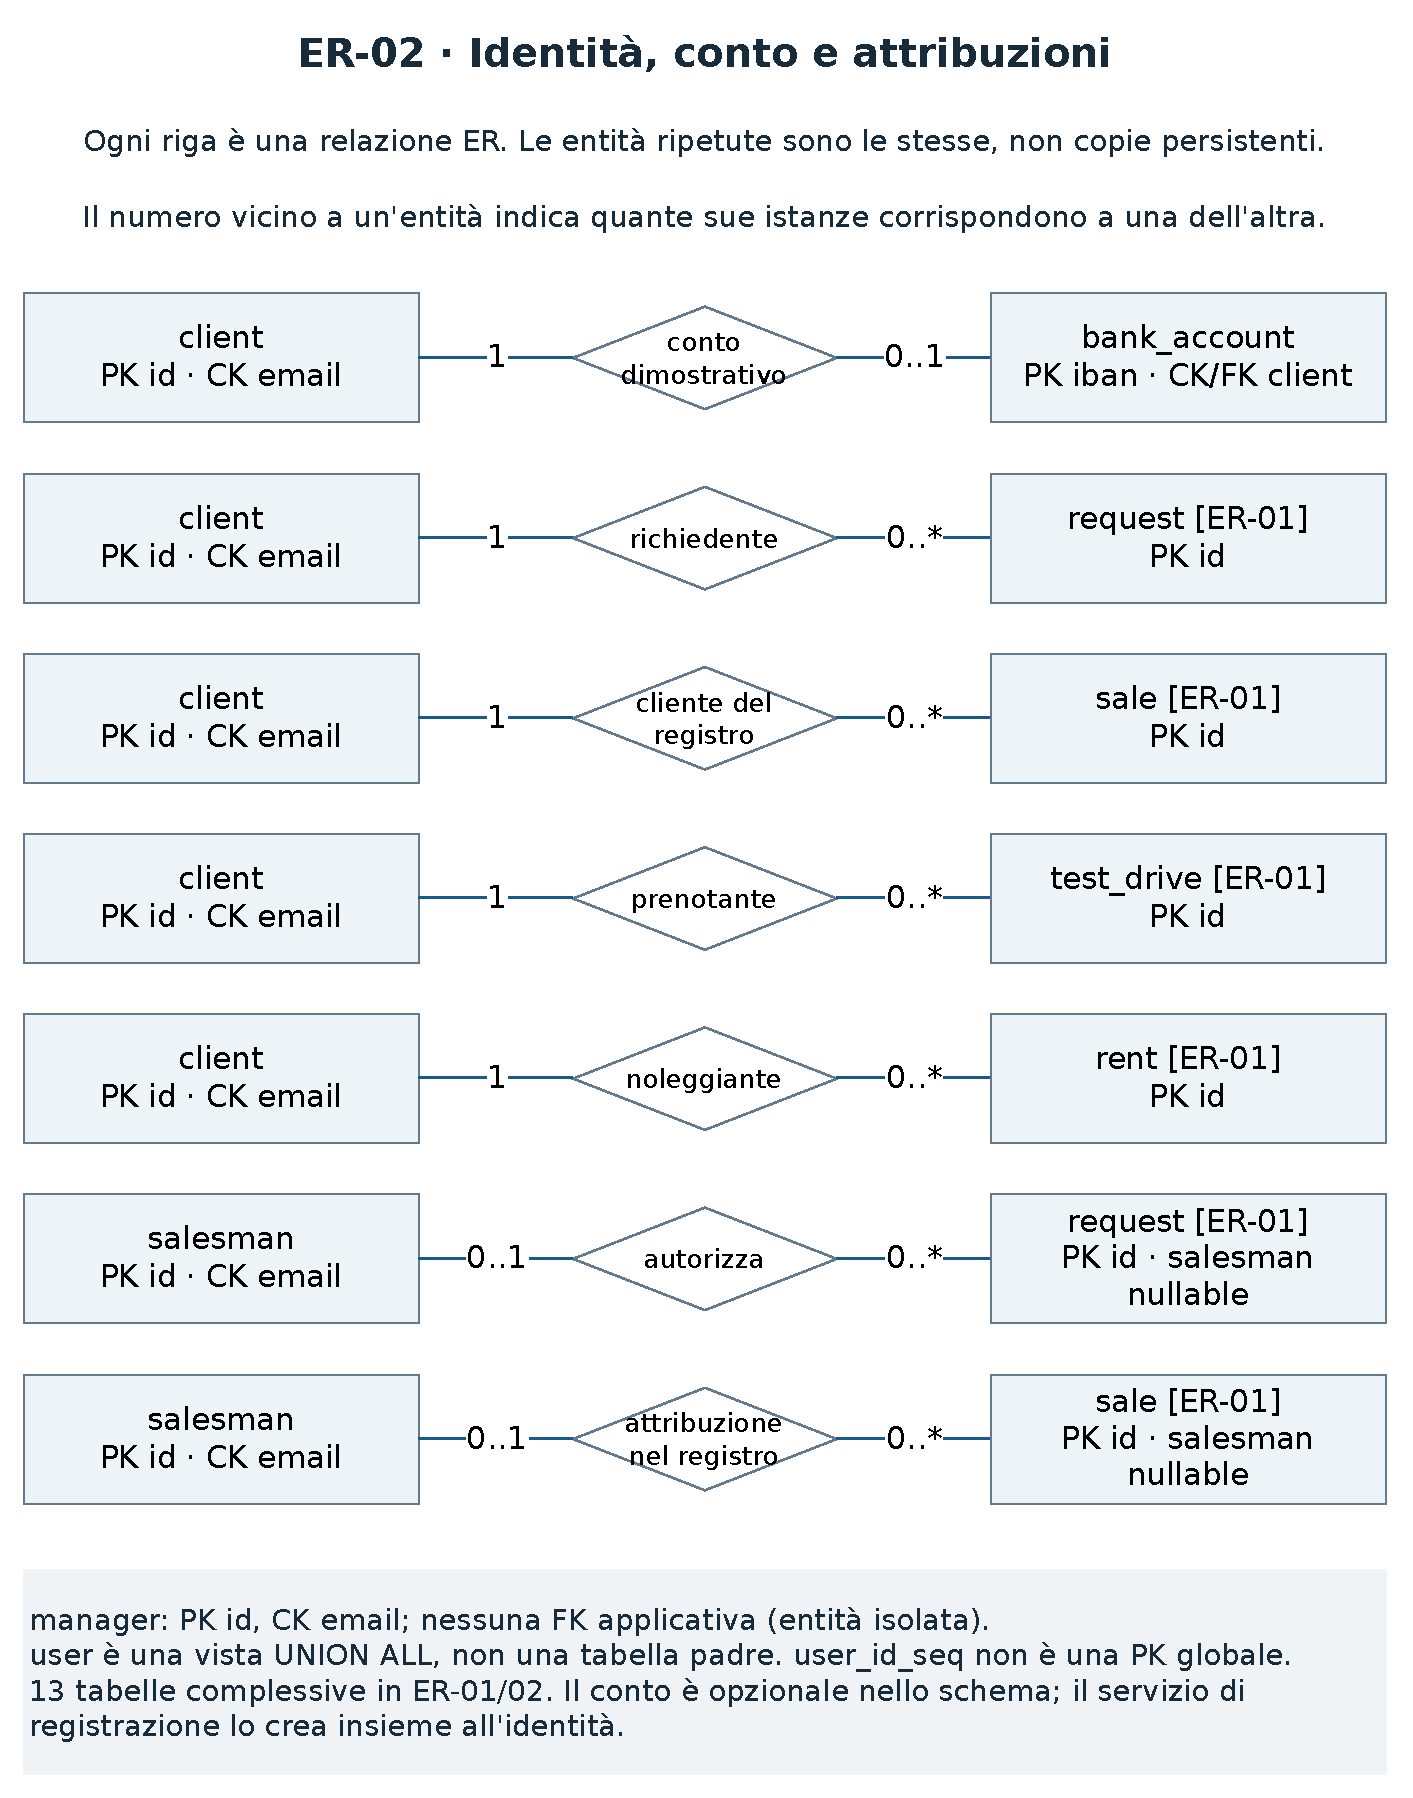
\includegraphics[width=\linewidth,height=.88\textheight,keepaspectratio]{diagrammi/database-er-identita.drawio.pdf}
  \caption{ER-02 --- Identità, conto e attribuzioni; le operazioni riprendono ER-01.}\label{fig:er02}
\end{figure}
\clearpage

\subsection{Modello relazionale}
REL-01--REL-03 (figure~\ref{fig:rel01}--\ref{fig:rel03}) riportano
tutti gli attributi, i tipi, le chiavi e i riferimenti. \code{PK} indica
la primaria; \code{CK} una candidata alternativa; \code{FK} un riferimento;
\code{?} la nullabilità. In assenza di \code{?} l'attributo è obbligatorio,
anche quando lo rende tale la primaria. Gli ID di catalogo e operazioni
sono \texttt{BIGINT GENERATED BY DEFAULT AS IDENTITY}; marca e conto
usano rispettivamente nome e IBAN. Gli sconti usano la FK come PK.

\noindent\textbf{Le tredici relazioni, nella notazione testuale.}
\code{PK} indica la primaria, \code{FK} la chiave esterna, \code{U} l'unicità.
Il suffisso \code{?} ammette \code{NULL}; tutti gli altri attributi sono
obbligatori. Una chiave può essere insieme \code{PK} e \code{FK}.
Gli importi sono \code{DECIMAL(10,2)}, gli ID \code{BIGINT}; tipi e lunghezze
completi sono nelle tavole REL. Il simbolo di unicità può riguardare anche
una combinazione di attributi, specificata dopo la relazione.
\begin{description}[style=nextline,leftmargin=1em]
\item[\code{brand}]
(\code{PK name}).
Nome fino a 50 caratteri, chiave usata dai modelli.
\item[\code{model}]
(\code{PK id}, \code{FK brand}, \code{U name}, \code{release_price}, \code{release_year}).
\code{brand} riferisce \code{brand.name}; nome unico globalmente, base non negativa e anno almeno 1900.
\item[\code{model_discount}]
(\code{PK/FK model}, \code{value}).
\code{model} riferisce \code{model.id}; una percentuale intera 0--50 per modello, facoltativa per il padre.
\item[\code{vehicle}]
(\code{PK id}, \code{FK model}, \code{U vin}, \code{U licence_plate?}, \code{kilometers}, \code{price}, \code{price_mode}, \code{year}, \code{state}).
\code{model} riferisce \code{model.id}. VIN fino a 17 caratteri, targa fino a 10; base e chilometri non negativi. \code{price_mode} è predefinito \code{AUTOMATIC}; stato e modalità usano enum distinti. Anno almeno 1900 e non prima del modello; targa assente solo a chilometri zero.
\item[\code{vehicle_discount}]
(\code{PK/FK vehicle}, \code{value}).
\code{vehicle} riferisce \code{vehicle.id}; una percentuale intera 0--50 per veicolo, facoltativa per il padre.
\item[\code{client}]
(\code{PK id}, \code{name}, \code{surname}, \code{U email}, \code{hash_password}).
Nome, cognome ed email fino a 50 caratteri, hash fino a 255. ID predefinito dalla sequenza \code{user_id_seq}; controllo minimo sulla forma dell'email.
\item[\code{salesman}]
(\code{PK id}, \code{name}, \code{surname}, \code{U email}, \code{hash_password}).
Stessi tipi, sequenza e controlli del cliente; primaria e unicità dell'email sono locali alla tabella del venditore.
\item[\code{manager}]
(\code{PK id}, \code{name}, \code{surname}, \code{U email}, \code{hash_password}).
Stessi tipi, sequenza e controlli del cliente; nessuna FK applicativa punta al manager.
\item[\code{bank_account}]
(\code{PK iban}, \code{FK/U client}, \code{balance}).
IBAN fino a 27 caratteri, cliente riferito a \code{client.id}; saldo non negativo, predefinito zero. L'unicità non impone un conto a ogni cliente.
\item[\code{request}]
(\code{PK id}, \code{FK/U vehicle}, \code{FK client}, \code{FK salesman?}, \code{deposit}, \code{agreed_total?}, \code{exp_date?}, \code{type}).
FK a \code{vehicle.id}, \code{client.id}, \code{salesman.id}. Una richiesta aperta per veicolo; scadenza \code{DATE}, tipo \code{request_type}. \code{SALE}: totale obbligatorio non negativo e acconto tra zero e totale; \code{PURCHASE}: stima non negativa e totale nullo.
\item[\code{test_drive}]
(\code{PK id}, \code{FK vehicle}, \code{FK client}, \code{date}).
FK a \code{vehicle.id} e \code{client.id}; data \code{TIMESTAMP}. \code{UNIQUE(vehicle,date)} rende unico il timestamp per veicolo; ora compresa fra 09:00 e 16:00 inclusi.
\item[\code{rent}]
(\code{PK id}, \code{FK vehicle}, \code{FK client}, \code{amount}, \code{start}, \code{end}).
FK a \code{vehicle.id} e \code{client.id}; importo non negativo, estremi \code{DATE} con fine non prima dell'inizio. \code{EXCLUDE} impedisce intersezioni degli intervalli inclusi per lo stesso veicolo.
\item[\code{sale}]
(\code{PK id}, \code{FK vehicle?}, \code{FK salesman?}, \code{FK client}, \code{amount}, \code{date}, \code{type}).
FK a \code{vehicle.id}, \code{salesman.id}, \code{client.id}; importo non negativo, data \code{TIMESTAMP}, tipo \code{sale_type}: \code{SALE}, \code{PURCHASE}, \code{PENALTY}. Nessuna FK alla richiesta consumata.
\end{description}
La vista \code{user(id,name,surname,email,hash_password,role)} combina le
identità con \code{UNION ALL}; il ruolo è una costante di ciascun ramo,
non una quattordicesima tabella. Nullabilità e azioni di cancellazione sono
proprietà distinte: una FK nullable non implica \code{SET NULL}.

Le candidate alternative sono \code{model.name}, \code{vehicle.vin},
le email all'interno di ciascuna tabella di ruolo,
\code{bank\_account.client}, \code{request.vehicle} e la coppia
\code{(vehicle,date)} del test drive: tutte sono uniche e non nulle.
Il nome del modello è unico globalmente, non soltanto entro una marca.
\code{vehicle.licence\_plate} ha invece un vincolo \code{UNIQUE} ed è
nullable: più valori nulli sono ammessi e non è una chiave candidata
dell'intera relazione. Le unicità testuali non implicano da sole
normalizzazione o confronto senza distinzione fra maiuscole e minuscole.

Le azioni \texttt{ON DELETE} sono specifiche. Gli sconti seguono in
\code{CASCADE} il proprio modello o veicolo; il conto segue il cliente.
\code{sale.vehicle} usa \texttt{SET NULL}, conservando la registrazione.
Le altre undici FK usano \code{RESTRICT}: marca con modelli, modello
con veicoli, riferimenti di richieste, test drive e noleggi, cliente e
venditore del registro. Di conseguenza un veicolo con un noleggio o un
test drive non è eliminabile per il solo fatto che \code{sale.vehicle}
consenta \texttt{SET NULL}. L'unico \texttt{ON UPDATE CASCADE} è
\code{model.brand}; le altre FK mantengono il predefinito \texttt{NO ACTION}.
I servizi aggiungono controlli conservativi sullo storico, senza cambiare
queste regole SQL.

\begin{figure}[p]
  \centering
  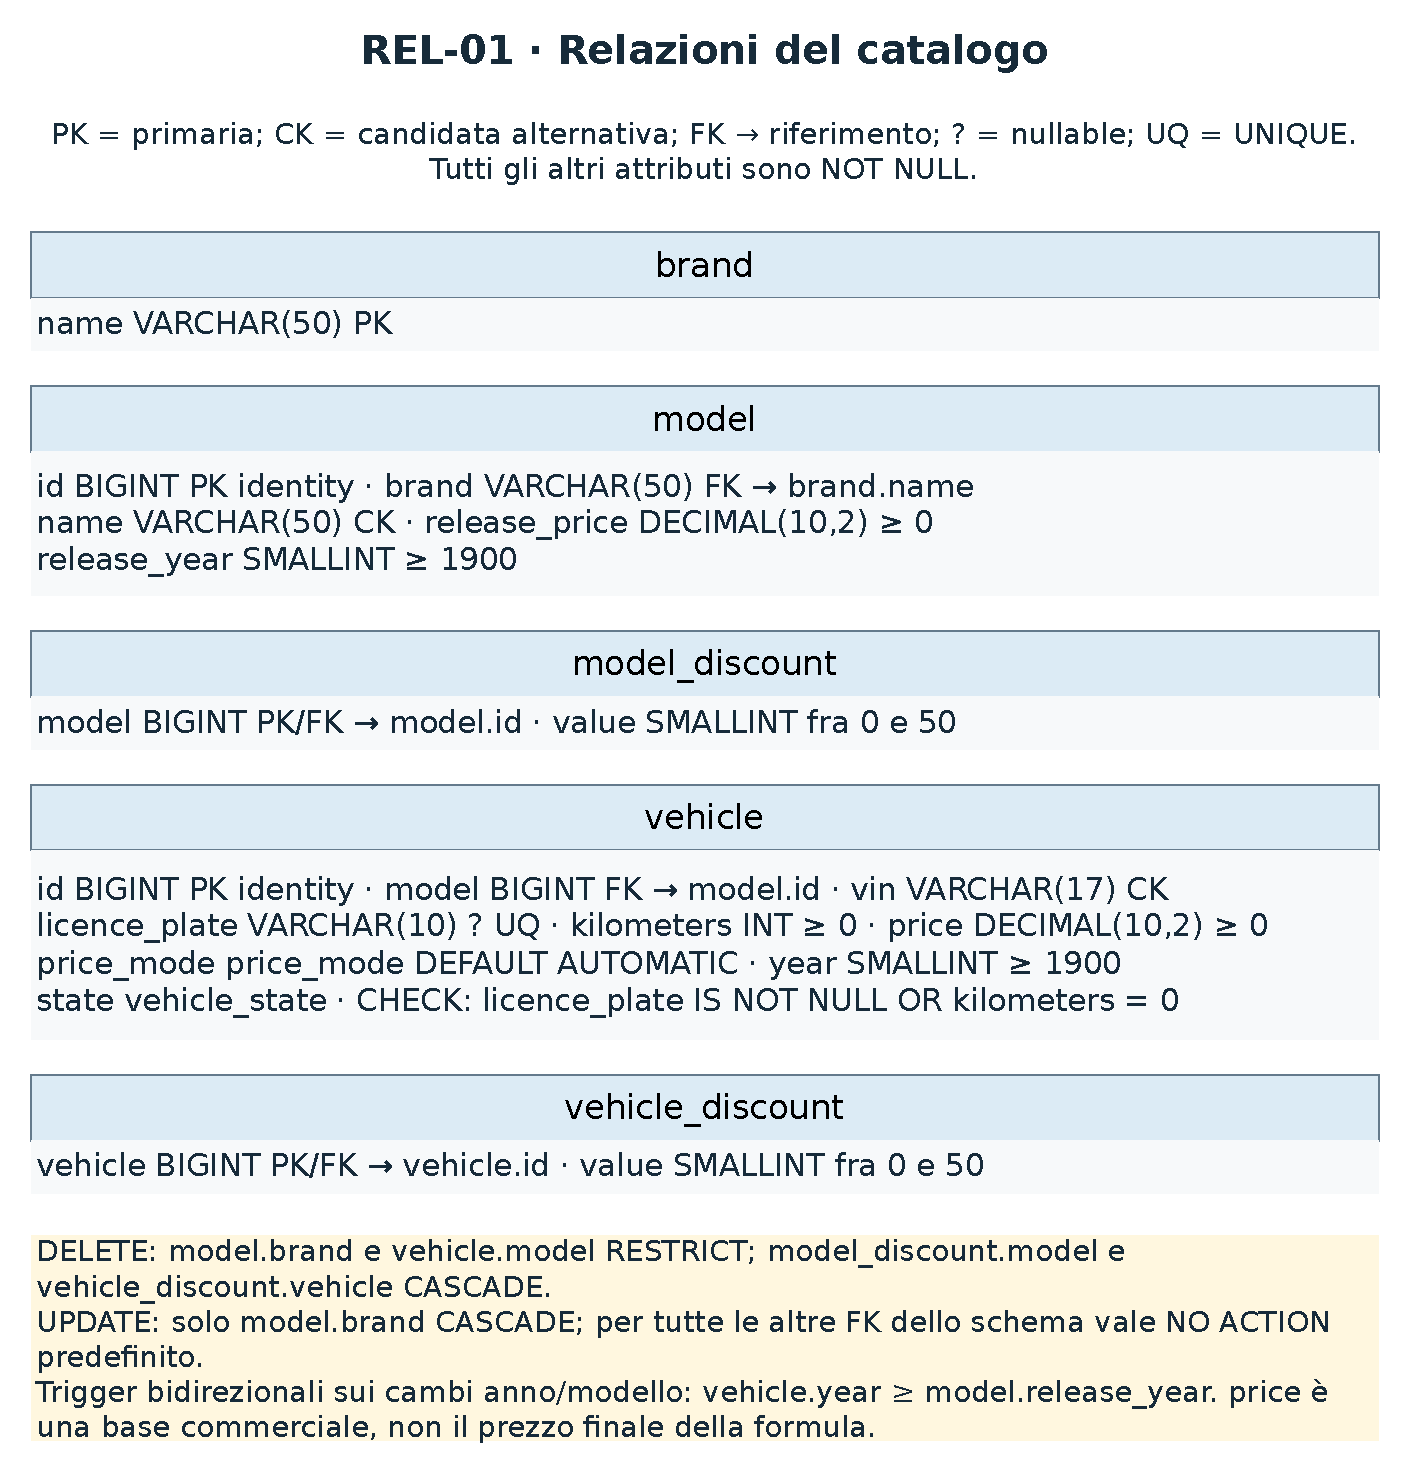
\includegraphics[width=\linewidth,height=.88\textheight,keepaspectratio]{diagrammi/database-relazionale-catalogo.drawio.pdf}
  \caption{REL-01 --- Attributi, chiavi e vincoli delle cinque tabelle del catalogo.}\label{fig:rel01}
\end{figure}
\begin{figure}[p]
  \centering
  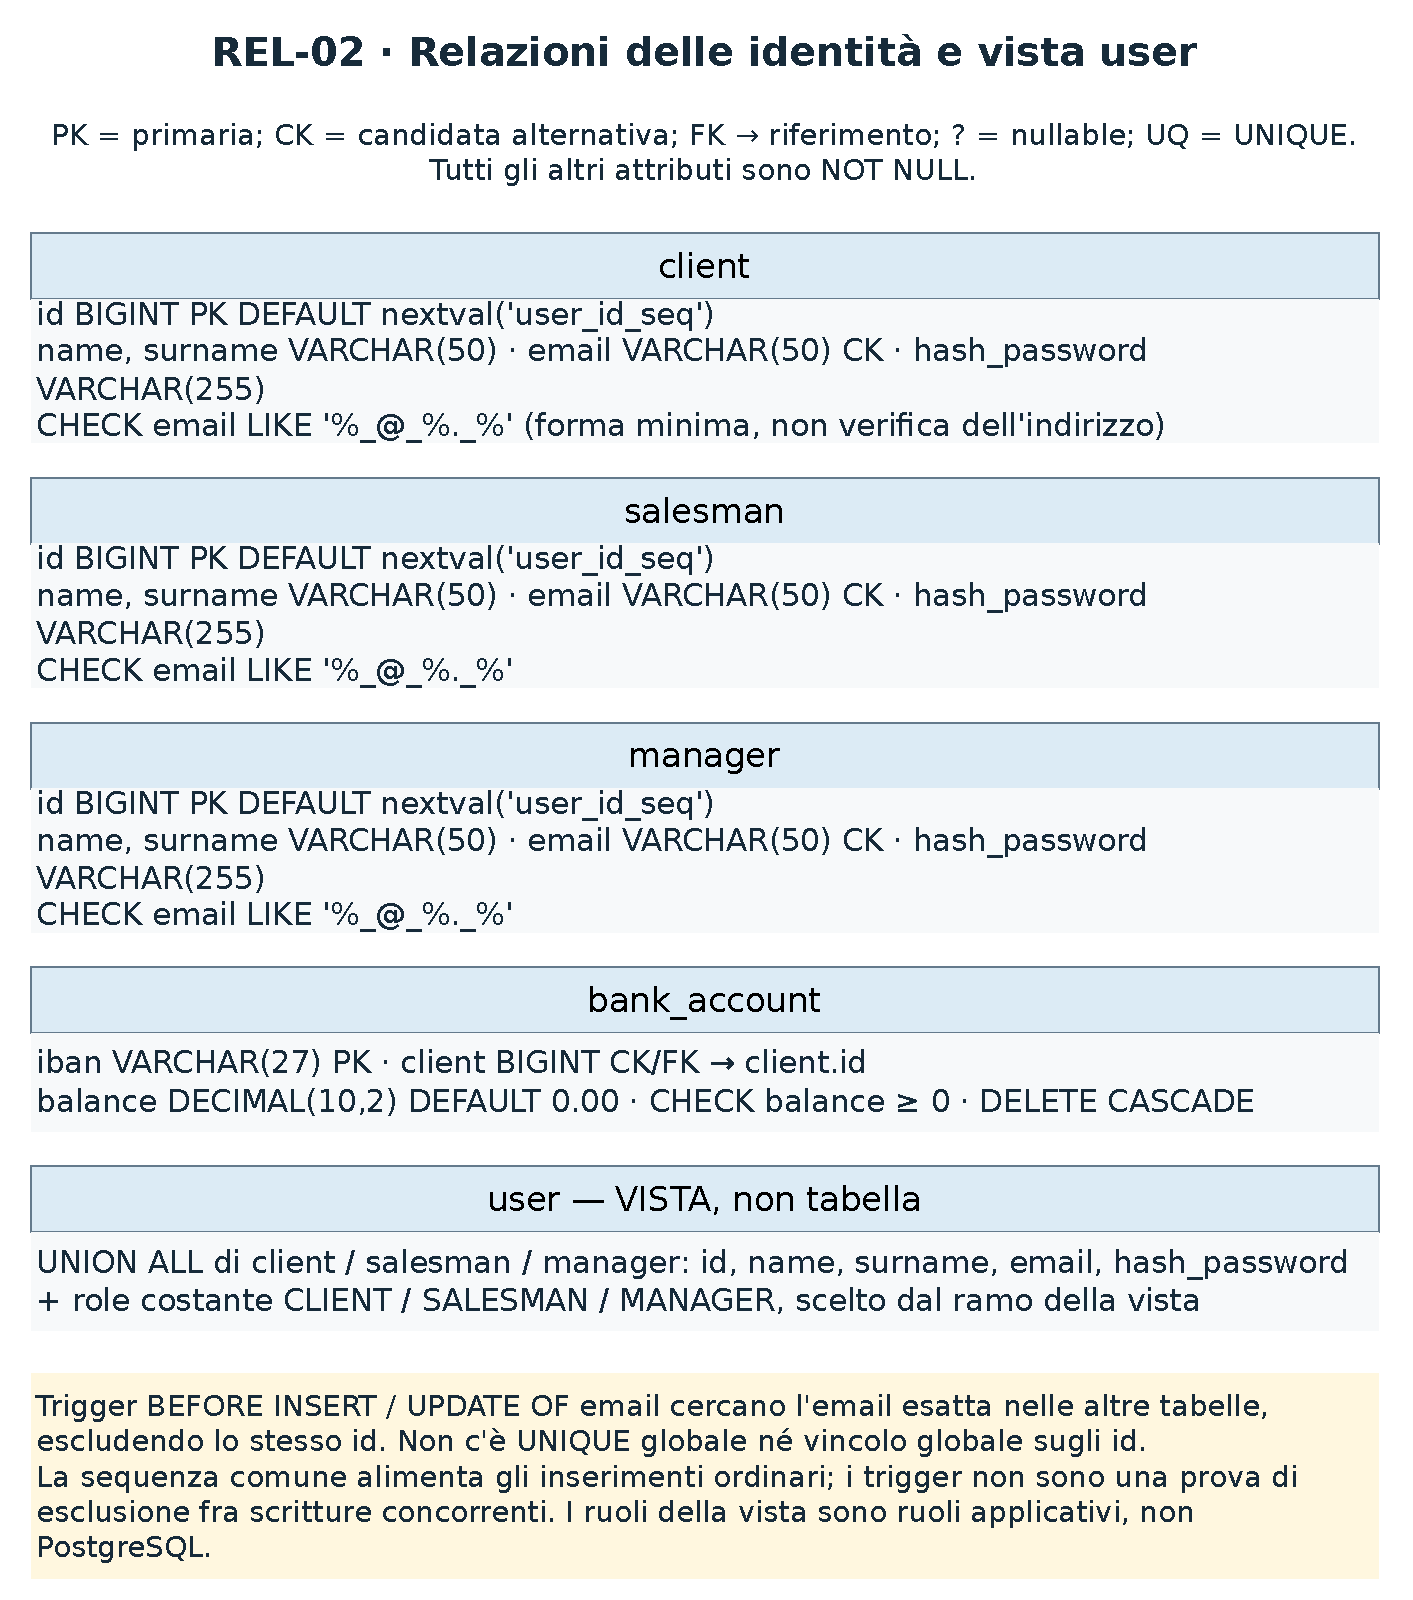
\includegraphics[width=\linewidth,height=.88\textheight,keepaspectratio]{diagrammi/database-relazionale-identita.drawio.pdf}
  \caption{REL-02 --- Tre tabelle di ruolo, conto dimostrativo e vista delle identità.}\label{fig:rel02}
\end{figure}
\begin{figure}[p]
  \centering
  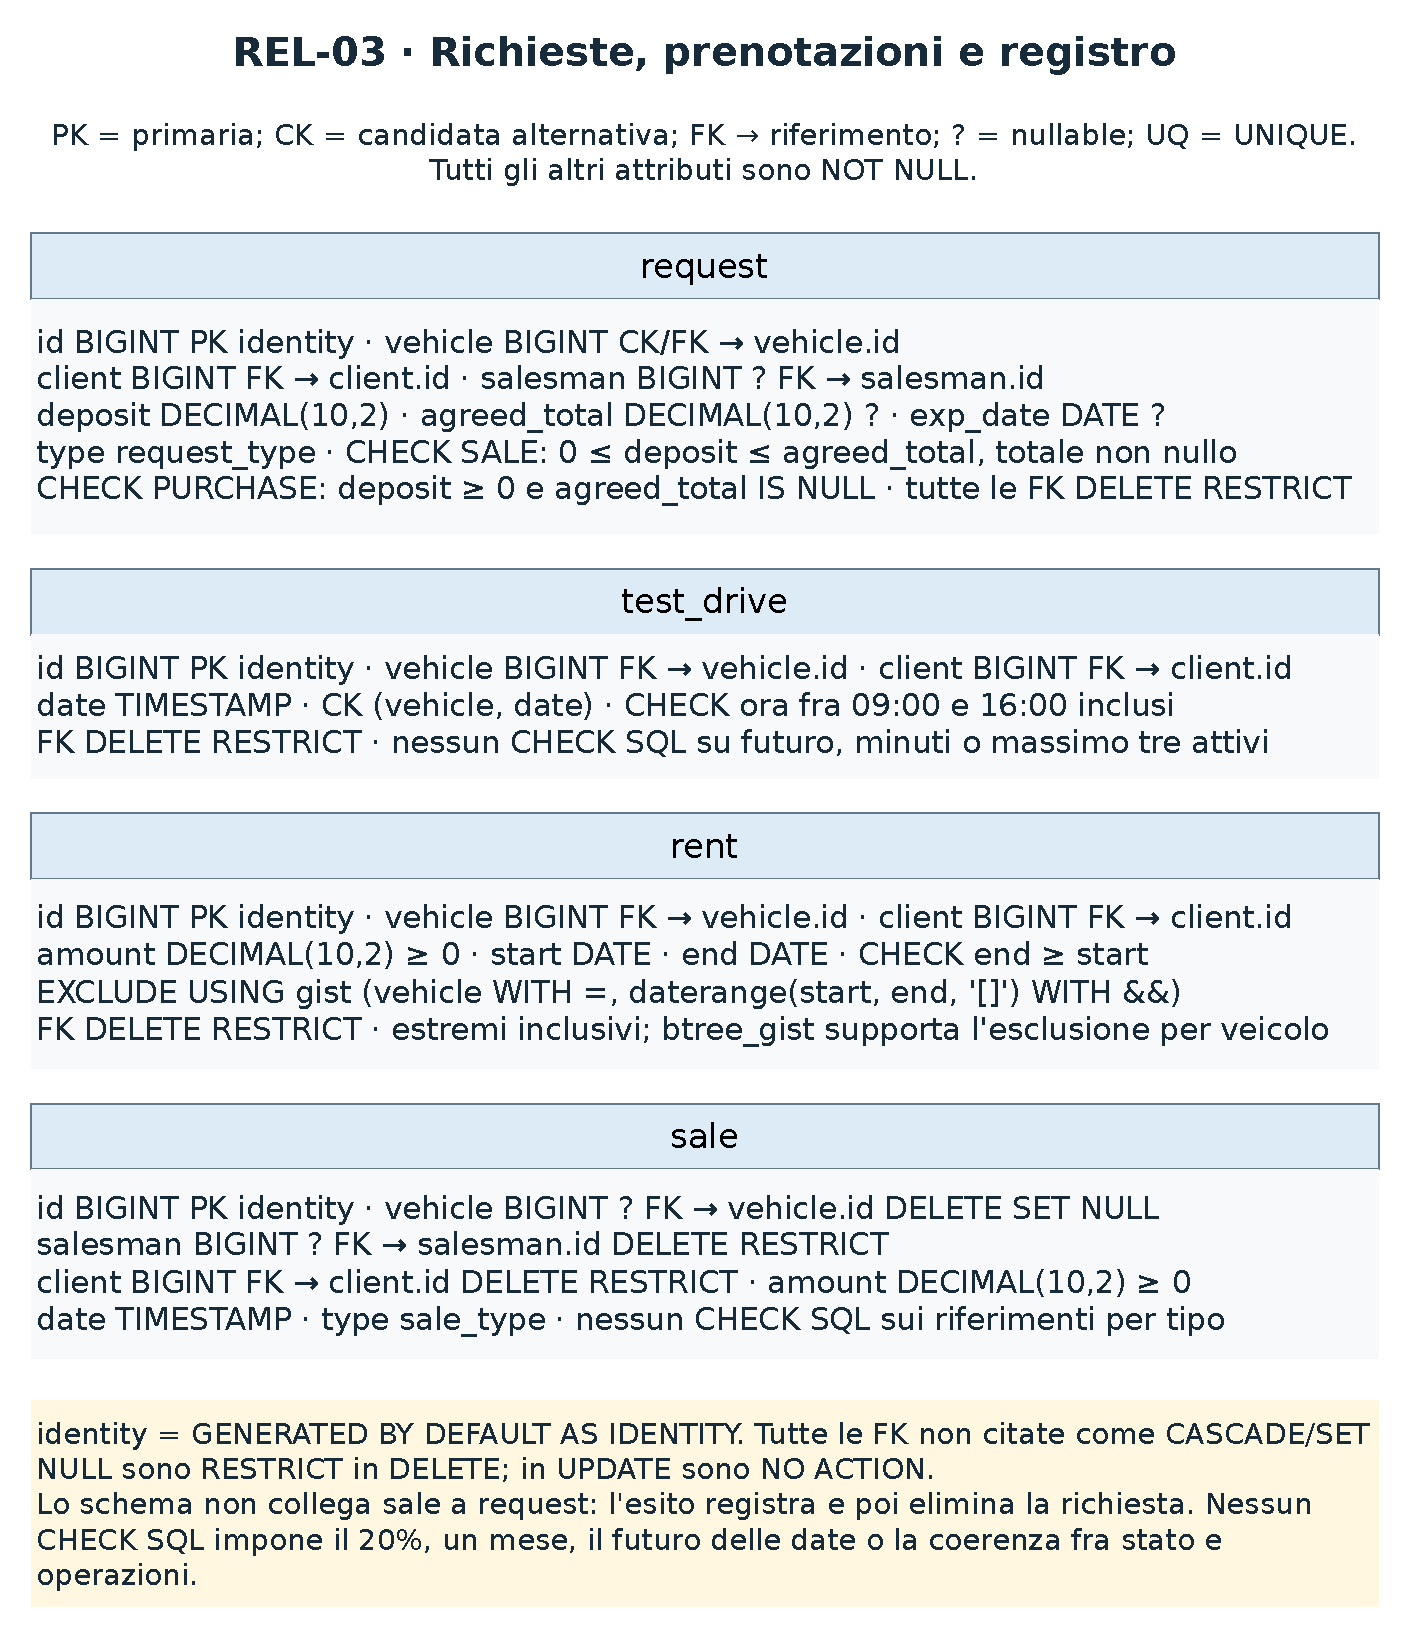
\includegraphics[width=\linewidth,height=.88\textheight,keepaspectratio]{diagrammi/database-relazionale-operazioni.drawio.pdf}
  \caption{REL-03 --- Richieste, test drive, noleggi e registro economico.}\label{fig:rel03}
\end{figure}
\clearpage

L'ADR~0002 mantiene quattro tipi enumerati nativi PostgreSQL, ciascuno
distinto. \code{vehicle\_state} ammette \code{SALE} (destinato alla
vendita al cliente), \code{RENT} (destinato al noleggio), \code{BLOCKED}
(riservato per la vendita al cliente), \code{WAITING} (proposta di cessione
in valutazione) e \code{SOLD} (venduto al cliente).
\code{request\_type} ammette \code{SALE} per la richiesta di vendita
al cliente e \code{PURCHASE} per quella di acquisto dal cliente.
\code{price\_mode} distingue \code{AUTOMATIC}, con base del modello,
da \code{MANUAL}, con base del veicolo nella stessa formula.
\code{sale\_type} distingue \code{SALE}, \code{PURCHASE} e
\code{PENALTY}: vendita al cliente, acquisto dal cliente e penale.
Il tipo esplicito determina il significato economico, anche a importo zero.
Non sono ruoli né stati di una richiesta. I DAO effettuano i cast JDBC
verso gli enum SQL e ricostruiscono gli enum Java; la scelta non richiede
qui nuove conversioni o migrazioni.

Gli importi persistenti usano \code{DECIMAL(10,2)}. I \code{CHECK}
impongono prezzi di rilascio e basi del veicolo, saldo, importo del
noleggio e importo del registro non negativi. Per \code{request},
\code{ck\_request\_agreement} distingue due forme: \code{SALE} richiede
totale non nullo, acconto non negativo e non superiore al totale;
\code{PURCHASE} richiede stima non negativa e totale nullo.
Il database non impone acconto del 20\%, immutabilità dell'accordo nel
tempo, associazione con lo stato del veicolo o corrispondenza fra scadenza
e venditore. Dominio e servizi fissano e utilizzano l'accordo come mostrato
in SQ-01a/SQ-01c. Il registro non ha una FK alla richiesta: conserva
l'esito economico mentre la richiesta viene eliminata.

Altri \code{CHECK} limitano sconti interi a 0--50, chilometri non
negativi, anni almeno 1900 e assenza di targa soltanto con chilometri zero.
I trigger sull'inserimento o modifica di anno/modello del veicolo e sulla
modifica dell'anno di rilascio del modello controllano
che l'anno del veicolo non preceda quello di rilascio del modello.
La presenza di questi controlli non prova un isolamento serializzabile
di ogni modifica concorrente fra tabelle.

Per la disponibilità, \code{rent} impone fine non precedente all'inizio
e un \texttt{EXCLUDE USING gist} sul veicolo e sull'intersezione di
\code{daterange(start,end,'[]')}, con estremi inclusi e supporto
\code{btree\_gist}. Due prenotazioni dello stesso veicolo non possono
condividere neppure un giorno. Il test drive rende unica la coppia
veicolo--timestamp e limita l'ora a 09:00--16:00 inclusi; non impone
slot interi di un'ora. Date future, limite di tre test drive attivi,
stato compatibile del veicolo e conflitto test drive--noleggio sono
controlli di dominio, servizi e query DAO, non vincoli SQL trasversali.
Le date del registro e dei test drive sono \code{TIMESTAMP} senza fuso;
quelle di noleggio e scadenza sono \code{DATE}. Il DDL non vieta date
nel passato né date future nel registro. Il mese per il saldo e
l'innesco della gestione delle scadenze restano applicativi.

\subsection{Utenti, vincoli e semplificazioni}
\guillemotleft{}Utenti\guillemotright{} indica le identità applicative, non account PostgreSQL.
\code{client}, \code{salesman} e \code{manager} ripetono gli attributi
comuni; la vista \code{user} ne combina le righe con \texttt{UNION ALL}
e aggiunge il ruolo costante del ramo. \code{PostgresUserDao} usa quel
ruolo per costruire il sottotipo Java e indirizzare le scritture.
La sequenza condivisa \code{user\_id\_seq} assegna normalmente ID
distinti, ma le PK sono locali e il DDL consente ID espliciti:
non esiste una primaria globale fra ruoli né una tabella padre che
imponga da sola una generalizzazione totale ed esclusiva.

Ogni tabella di ruolo ha email obbligatoria e unica e un controllo
minimo di forma con \code{LIKE}. I trigger cercano email uguali nelle
altre due tabelle durante inserimento e modifica dell'email, escludendo
righe con lo stesso ID. Sono controlli procedurali, non un indice unico
globale: non dimostrano esclusione di scritture concorrenti e non
impediscono il caso di ID espliciti coincidenti. Il confronto SQL dei
vincoli è testuale, mentre la ricerca di accesso usa \code{LOWER(email)};
non si presenta quindi l'intero sistema come un'unicità globale senza
distinzione di maiuscole. Questi limiti sono segnalati separatamente,
senza introdurre uno schema alternativo.

Le password sono rappresentate da hash, non da credenziali in chiaro
nel modello documentato. La registrazione ordinaria crea solo un cliente
e il relativo conto a saldo zero nella stessa transazione.
Il conto ha IBAN come chiave, un solo cliente e saldo non negativo;
è una simulazione locale, senza collegamento bancario, verifica di
titolarità reale o registro separato di tutti i movimenti. Il formato
dell'IBAN è controllato dal dominio, mentre il DDL ne limita lunghezza
e unicità. La cancellazione del cliente elimina il conto per
\code{CASCADE}, anche se positivo, ma richieste e operazioni storiche
possono impedirla con le loro FK. L'accesso JDBC usa la connessione
configurata per l'applicazione: il DDL non crea un ruolo PostgreSQL per
ogni cliente, venditore o manager e non definisce politiche per riga.

Le scelte privilegiano un archivio didattico compatto, mapping JDBC
esplicito e riferimenti storici conservati. Non costituiscono una
contabilità bancaria completa né una garanzia generale di autorizzazione
o concorrenza. Schema corrente e quattro enum restano quelli consegnati,
coerenti con gli ADR~0001 e~0002; nessuna migrazione o conversione è
introdotta dalla relazione. Il capitolo 2 è ora completo e proposto,
con le appendici A--B, per la revisione degli autori; tale revisione
non è già approvata.

\endgroup

\setcounter{secnumdepth}{2}

\chapter{Implementazione}\label{ch:implementazione}
Il capitolo collega le scelte del progetto a porzioni selezionate dei sorgenti
correnti. Le tavole delle classi in appendice~\ref{app:classi}, le sequenze
della sezione~\ref{sec:sequenze} e il modello dati della
sezione~\ref{sec:database} restano i riferimenti d'insieme: qui interessa
capire dove sono applicate le regole e fin dove valgono.
I frammenti sono estratti letterali degli intervalli indicati nei sorgenti,
con numerazione originale: omettono il contesto esterno, descritto nel testo.
Non sono programmi completi né pseudocodice; eventuali selezioni interne
sono dichiarate presso l'esempio. Il capitolo è proposto alla revisione
degli autori, senza attribuirne l'approvazione.

\begingroup
\setcounter{secnumdepth}{3}
\emergencystretch=6em
\renewcommand{\lstlistingname}{Frammento}
\lstset{language=Java,basicstyle=\ttfamily\footnotesize,
  columns=fullflexible,keepspaces=true,showstringspaces=false,
  breaklines=true,breakatwhitespace=false,tabsize=4,gobble=4,upquote=true,
  numbers=left,numberstyle=\tiny\color{black!60},numbersep=8pt,
  frame=lines,rulecolor=\color{black!25},captionpos=b,
  aboveskip=9pt,belowskip=9pt,
  literate={à}{{\`a}}1 {è}{{\`e}}1 {é}{{\'e}}1
    {ì}{{\`i}}1 {ò}{{\`o}}1 {ù}{{\`u}}1
    {…}{{\normalfont\textellipsis}}1}
\section{Domain Model}\label{sec:impl-dominio}
Il modello usa i package \code{domain.user}, \code{domain.vehicle},
\code{domain.discount} e \code{domain.operation}. Manteniamo i cinque gruppi
espositivi originali: Users, Vehicles, Rentals, Sales e contratto Observer;
l'ultimo appartiene ora al package separato \code{event}.
La figura~\ref{fig:catalogo-corpo} e i dettagli CL in
appendice~\ref{app:classi} distinguono ereditarietà, riferimenti a oggetti
e semplici ID. Non esiste più \code{BaseEntity.assignId}: un ID nullo può
indicare un oggetto da inserire; i DAO restituiscono un nuovo oggetto identificato.

\subsection{Users}
La gerarchia \code{User}/\code{AbstractUser} condivide identificativo,
nome, cognome, email e hash della password; \code{Client}, \code{Salesman}
e \code{Manager} specializzano ruolo e apertura della dashboard.
\code{AbstractUser} è una classe astratta con costruttore protetto.
Nome e cognome sono finali e ripuliti con trim, email e hash aggiornabili
con validazione. L'email è normalizzata in minuscolo e verificata con una
regex; nome, cognome e hash devono essere non vuoti. La validità sintattica
di un oggetto non prova che l'email sia libera nei dati persistenti.

\code{equals} richiede la stessa classe concreta: confronta gli ID quando
entrambi presenti e l'email quando entrambi assenti. Non identifica per
sola email due utenti persistiti né un cliente e un venditore con lo stesso
numero. La selezione della tabella per ruolo e il limite della ricerca
comune per solo ID sono ripresi in~\ref{sec:impl-utenti-sql}.
\code{Client} contiene un riferimento opzionale e sostituibile a
\code{BankAccount}, caricato anche dopo l'autenticazione: non è una
composizione UML deducibile dal solo campo.

\code{BankAccount} conserva IBAN e ID cliente finali e saldo modificabile.
La factory richiede cliente non nullo, saldo non negativo e IBAN normalizzato
con due lettere, due cifre e da 11 a 30 caratteri alfanumerici successivi:
non impone esattamente 27 caratteri né controlla la cifra bancaria di verifica.
\code{createInitial} parte da zero. \code{deposit} e \code{withdraw}
richiedono importi strettamente positivi; il prelievo verifica la capienza
prima di sottrarre, lasciando invariato il saldo se fallisce. L'identità
del conto dipende dall'IBAN. Si tratta di regole in memoria: lock della riga,
unicità e salvataggio del saldo sono responsabilità persistenti, non effetti
automatici dei mutatori. Non c'è collegamento a una banca esterna.

\subsection{Vehicles}
\code{Brand} è identificata dal nome non vuoto e ripulito;
\code{Model} conserva ID, marca, nome, prezzo e anno di rilascio.
La marca è un nome scalare, non un oggetto caricato automaticamente.
La validazione di prezzo non negativo e anno fra 1900 e anno corrente
precede la costruzione. I campi di \code{Model}, inclusi prezzo e anno,
sono finali: una modifica persistente non è una mutazione di quell'istanza. La gerarchia \code{Discount}
riusa nel costruttore il controllo inclusivo 0--50; \code{ModelDiscount}
e \code{VehicleDiscount} conservano ID del bersaglio e percentuale finali.
L'unico sconto per bersaglio è anche una proprietà delle chiavi SQL.

\code{Vehicle} è una classe finale con costruttore privato: la factory
\code{create} controlla i dati prima di costruire l'oggetto. ID, modello,
VIN e anno sono campi finali; targa, chilometri, base del prezzo, modalità
e stato possono cambiare. Il frammento~\ref{lst:vehicle-invariante}
mostra una regola che riguarda due attributi, anziché due controlli
indipendenti.

% Fonte: src/main/java/it/unifi/drivehub/domain/vehicle/Vehicle.java:59-62
\noindent\begin{minipage}{\linewidth}
\begin{lstlisting}[firstnumber=59,caption={\code{Vehicle.java}: normalizzazione della targa e coerenza con i chilometri.},
  label=lst:vehicle-invariante]
        String cleanPlate = (licencePlate != null && !licencePlate.trim().isEmpty()) ? licencePlate.trim().toUpperCase() : null;
        if (cleanPlate == null && kilometers != 0) {
            throw new IllegalArgumentException("Se un veicolo non ha targa, obbligatoriamente i chilometri devono essere 0.");
        }
\end{lstlisting}
\end{minipage}


La stessa coerenza è controllata dai mutatori: per rimuovere la targa occorre
prima portare i chilometri a zero. La factory rifiuta chilometri e prezzo
negativi, anno fuori dall'intervallo 1900--anno corrente, modello o stato
nulli. Il VIN viene ripulito e convertito in maiuscolo; il controllo
effettivo ammette da uno a diciassette caratteri dopo il trim, senza imporre
diciassette caratteri esatti o verificarne l'alfabeto. L'unicità appartiene
al database. Il confronto con l'anno del modello richiede
\code{validateProductionYear}, invocato dal servizio di catalogo, ed è
anche presidiato dai trigger SQL. Il solo \code{setState} rifiuta null:
non codifica un automa di transizioni; sono i servizi a verificare gli stati
ammessi nei singoli comandi.

Lo stato locale \code{VehicleState} comprende \code{WAITING}, \code{SALE},
\code{RENT}, \code{BLOCKED} e \code{SOLD}. L'esempio originale di
\code{approve}/\code{block} è sostituito dall'invariante locale sopra e
dall'UPDATE condizionale del frammento~\ref{lst:update-condizionale}:
la classe non impone un automa, il servizio decide la transizione e il DAO
ne verifica atomicamente la precondizione persistita.
\code{PriceMode.AUTOMATIC}/\code{MANUAL} sceglie la base del calcolo,
come spiegato in~\ref{sec:impl-prezzi}; non aggiunge uno stato commerciale.
L'uguaglianza di Model usa l'ID se entrambi gli oggetti sono identificati,
altrimenti marca/nome se entrambi ne sono privi; Vehicle usa analogamente
ID oppure VIN. Un oggetto nuovo e uno persistito non diventano uguali
per il solo nome o VIN. Questi confronti in memoria non aggiungono
unicità al database né mantengono un'unica istanza Java per riga.

\subsection{Rentals}
\code{Rent} e \code{TestDrive} sono in \code{domain.operation}, senza
gli antichi package rentals separati. Conservano ID di cliente e veicolo,
non riferimenti caricati. \code{Rent} richiede importo non negativo,
entrambe le date \code{LocalDate} e fine non precedente all'inizio.
I campi sono finali; \code{overlapsWith} considera inclusi entrambi gli
estremi e \code{isFuture} richiede inizio successivo a oggi. La factory
non vieta da sola una data passata: il servizio di prenotazione la rifiuta.

\code{TestDrive} conserva un \code{LocalDateTime} finale, con inizio
fra le 09:00 e le 16:00 incluse. Prima delle 16 ammette anche minuti,
secondi e frazioni: alle 16 richiede invece minuto, secondo e nanosecondo
zero. Un input 15:30 è quindi valido nel dominio; 16:00:01 è rifiutato.
La UI propone ore intere, ma il servizio non tronca un input alternativo.
Non esiste un campo fine o un metodo che realizzi una durata di un'ora:
la query confronta lo stesso istante e il giorno del noleggio.

Nessuna delle due entità può impedire da sola conflitti con altre righe.
La regola dei tre test drive attivi, la disponibilità, i lock e le
garanzie SQL si spiegano nei flussi~\ref{sec:impl-flussi} e
nei vincoli~\ref{sec:impl-vincoli}; un oggetto valido in memoria può
ancora essere rifiutato al salvataggio.

\subsection{Sales}
\code{Request} mantiene finali tipo, ID di richiesta, veicolo e cliente,
acconto e totale;
venditore e scadenza sono aggiornabili. Le due interpretazioni economiche
del campo \code{deposit} dipendono da \code{RequestType}: con \code{SALE}
è l'acconto della vendita al cliente; con \code{PURCHASE} è la stima per
l'acquisto dal cliente, senza totale concordato.

% Fonte: src/main/java/it/unifi/drivehub/domain/operation/Request.java:54-65
\noindent\begin{minipage}{\linewidth}
\begin{lstlisting}[firstnumber=54,caption={\code{Request.java}: forma dell'accordo e precisione degli importi.},
  label=lst:request-accordo]
        if (type == RequestType.SALE) {
            if (agreedTotal == null || agreedTotal.signum() < 0
                    || deposit.compareTo(agreedTotal) > 0) {
                throw new IllegalArgumentException("Totale concordato e acconto non validi per l'acquisto.");
            }
            // Gli importi dell'accordo devono essere già espressi in centesimi, come l'addebito.
            agreedTotal = agreedTotal.setScale(2, RoundingMode.UNNECESSARY);
            deposit = deposit.setScale(2, RoundingMode.UNNECESSARY);
        } else if (agreedTotal != null) {
            throw new IllegalArgumentException("Il totale concordato riguarda solo gli acquisti del cliente.");
        }
        return new Request(id, vehicleId, clientId, salesmanId, deposit, agreedTotal, expDate, type);
\end{lstlisting}
\end{minipage}


I controlli precedenti a questo estratto rifiutano acconto/stima negativi
e ID di veicolo o cliente nulli. \code{UNNECESSARY} accetta solo importi
rappresentabili in centesimi senza arrotondamento; non corregge un valore
più preciso. \code{getRemainingAmount} sottrae l'acconto dal totale solo
per \code{SALE}. La ricostruzione tramite \code{create} accetta una
scadenza già passata: serve a leggere richieste persistite da elaborare.
È il mutatore \code{setExpDate} a rifiutare una nuova scadenza passata;
\code{isExpired} confronta la data con oggi, escluso oggi stesso.

Le factory nominate rendono esplicita l'interpretazione economica:
vendita della concessionaria con totale/acconto, oppure acquisto dal
cliente con stima. L'estratto è letterale e completo per i due metodi:
non conserva la vecchia codifica della stima con segno negativo.

% Fonte: src/main/java/it/unifi/drivehub/domain/operation/Request.java:68-74
\noindent\begin{minipage}{\linewidth}
\begin{lstlisting}[firstnumber=68,gobble=4,caption={Factory dei due tipi di pratica, senza codifica del segno.},label=lst:request-factory]
    public static Request createNewSaleRequest(Long vehicleId, Long clientId, BigDecimal deposit, BigDecimal agreedTotal) {
        return create(null, vehicleId, clientId, null, deposit, agreedTotal, null, RequestType.SALE);
    }

    public static Request createNewPurchaseRequest(Long vehicleId, Long clientId, BigDecimal estimatedValue) {
        return create(null, vehicleId, clientId, null, estimatedValue, null, null, RequestType.PURCHASE);
    }
\end{lstlisting}
\end{minipage}

\code{Sale} registra esiti economici, mentre \code{Request} descrive
una pratica aperta. Ha campi finali, importo non negativo, cliente e
\code{SaleType} obbligatori. \code{SALE}, \code{PURCHASE} e \code{PENALTY}
indicano il verso economico dal punto di vista della concessionaria,
senza dedurlo dal segno. La factory della penale passa veicolo e venditore
nulli; quella generale non impone tutte le combinazioni possibili fra tipo
e riferimenti. La data deve essere presente: il codice tollera fino a due
minuti nel futuro, non vieta ogni scarto rispetto all'orologio corrente.
FK e controlli dei servizi completano le invarianti; l'esistenza di una
\code{Sale} associata non basta a provare la titolarità corrente del veicolo.

{\raggedright
\subsection{Eventi e contratto Observer}
\code{VehicleCommitmentEvent} è un record che trasporta il solo
\code{vehicleId}; \code{VehicleCommitmentObserver} riceve evento e
\code{Connection}; \code{VehicleEventPublisher} gestisce iscrizione,
rimozione e notifica. Sono tutti nel package \code{event}, separato da
\code{domain}: non si ripristina il vecchio gruppo \code{domain.observer}.
L'evento rappresenta l'impegno commerciale per vendita completata o
noleggio; non contiene targa, vecchio/nuovo stato o timestamp.
Il contratto letterale è in~\ref{lst:contratto-observer}; l'effetto
concreto e il confine prima del commit sono discussi
in~\ref{sec:impl-observer}. La presenza di una Connection nel contratto
rende esplicita la dipendenza JDBC, senza trasformare il record in una
notifica persistente.\par}


\section{Business Layer}\label{sec:impl-business}
I servizi del package \code{service} coordinano entità e DAO; sicurezza
ed eventi sono package distinti. La figura~\ref{fig:eventi-corpo} mostra
i collaboratori attuali. Riprendiamo coordinamento, responsabilità e
quattro flussi prima di formule, identità e politica Observer.

\subsection{Coordinamento e transazioni}\label{sec:impl-transazioni}
\code{DatabaseManager} apre una connessione per ogni esecuzione
transazionale. Il frammento~\ref{lst:transazione} mostra il percorso con
risultato; quello senza risultato applica lo stesso schema.

% Fonte: src/main/java/it/unifi/drivehub/dao/DatabaseManager.java:88-106
\noindent\begin{minipage}{\linewidth}
\begin{lstlisting}[firstnumber=88,caption={\code{DatabaseManager.java}: commit, tentativo di rollback e conservazione delle cause.},
  label=lst:transazione]
    public <T> T executeInTransactionWithResult(TransactionFunction<T> function) {
        try (Connection conn = getConnection()) {
            conn.setAutoCommit(false);
            try {
                T result = function.execute(conn);
                conn.commit();
                return result;
            } catch (Exception e) {
                try {
                    conn.rollback();
                } catch (SQLException rollbackEx) {
                    e.addSuppressed(rollbackEx);
                }
                throw new RuntimeException("Transazione fallita: eseguito rollback.", e);
            }
        } catch (SQLException e) {
            throw new RuntimeException("Errore di connessione al database durante la transazione.", e);
        }
    }
\end{lstlisting}
\end{minipage}


Il valore torna al chiamante dopo \code{commit}; il try-with-resources
chiude la connessione. Le eccezioni del corpo o del commit raggiungono
il ramo di rollback, poi sono incapsulate con la causa. Un errore del
rollback è aggiunto come eccezione soppressa: il testo del messaggio
non dimostra che il rollback sia riuscito. Il codice intercetta
\code{Exception}, non ogni \code{Error}; un guasto di rete durante il
commit non permette di dedurne sempre l'esito dal client. Non vi sono
retry automatici o transazioni annidate implicite.

{\raggedright
Le due callback annidate sono tipi distinti: \code{TransactionConsumer}
serve a \code{executeInTransaction}, \code{TransactionFunction<T>}
a \code{executeInTransactionWithResult}. Entrambe ricevono la Connection
aperta dal gestore e possono propagare \code{Exception}; la seconda
restituisce il valore della lambda, reso disponibile dopo il commit.\par}


% Fonte: src/main/java/it/unifi/drivehub/dao/DatabaseManager.java:53-60
\noindent\begin{minipage}{\linewidth}
\begin{lstlisting}[firstnumber=53,gobble=4,caption={Due callback distinte con Connection e risultato.},label=lst:callback]
    @FunctionalInterface
    public interface TransactionConsumer {
        void execute(Connection conn) throws Exception;
    }

    @FunctionalInterface
    public interface TransactionFunction<T> {
        T execute(Connection conn) throws Exception;
\end{lstlisting}
\end{minipage}

Il chiamante non possiede un'unità di lavoro implicita o un contesto JDBC
globale: deve passare realmente \code{conn} a ogni operazione partecipante.
\code{getConnection} usa \code{DriverManager.getConnection} e apre una
nuova connessione a ogni chiamata; non è un pool. Il gestore disabilita
autocommit per la transazione, ma non imposta un livello di isolamento.
Non attribuiamo quindi serializzabilità o snapshot unico al solo wrapper.

Le \code{SQLException} di apertura, di \code{setAutoCommit} o di chiusura
seguono il wrapper esterno. Se la chiusura fallisce mentre è già in corso
una propagazione, try-with-resources conserva il guasto come eccezione
soppressa; se fallisce dopo un commit riuscito il chiamante può ricevere
un errore pur con scritture già confermate. Una seconda chiamata del
gestore apre un'altra transazione: non esistono annidamento automatico,
retry o rollback di effetti esterni. I lock dei singoli servizi completano
il coordinamento e non dimostrano assenza generale di deadlock.

{\raggedright
\subsection{Services: responsabilità}
\begin{itemize}
\item \code{AuthService}: Login, registrazione del solo cliente con conto,
modifiche dell'identità, cancellazione e ricarica dimostrativa; collabora
con UserDao, BankAccountDao, PasswordHasher e DatabaseManager.
\item \code{CatalogService}: Letture e manutenzione di marche, modelli,
veicoli, basi e sconti tramite i relativi DAO; prepara le righe di catalogo
con PriceCalculatorService, senza demandare query alle celle JavaFX.
\item \code{OperationQueryService}: Consultazione di richieste, test drive,
noleggi e registro tramite RequestDao, TestDriveDao, RentDao e SaleDao;
non è il servizio che completa le operazioni economiche.
\item \code{PriceCalculatorService}: Formule centralizzate per consigliato,
effettivo, acconto, tariffa, costo e stima; riceve dati, non esegue SQL.
\item \code{PurchaseService}: Vendita al cliente: avvio, esito del venditore,
saldo e scadenza, con veicolo, modello/sconti, richiesta, conto, registro,
calcolatore e publisher.
\item \code{RentalService}: Preventivo, prenotazione e cambio di destinazione
SALE/RENT, con rimborsi dei futuri; usa anche UserDao per il lock del cliente.
\item \code{SaleToDealershipService}: Stima, proposta di cessione ed esito:
coordina veicolo, modello/sconto modello, richiesta, conto e storico Sale.
\item \code{TestDriveService}: Prenotazione, consultazione e cancellazione
del proprio test drive; coordina veicolo, cliente e disponibilità persistita.
\end{itemize}
\code{AppContext} costruisce esplicitamente questi collaboratori e registra
\code{TestDriveCancellationObserver}. Non ci sono gli antichi servizi
PricingService/BankAccountService né una DaoFactory/UnitOfWork.
La DI manuale consente di leggere le dipendenze, ma servizi e contratti
DAO restano legati a Connection; il contesto sceglie adapter PostgreSQL
e PBKDF2 concreti.\par}


\subsection{Services: flussi applicativi}\label{sec:impl-flussi}
Ogni comando seguente ha un ingresso distinto e un proprio confine
transazionale. I rinvii alle sequenze del capitolo 2 completano la lettura
delle decisioni e delle alternative, senza sostituirle.

\subsubsection{Catalogo e test drive}
La dashboard legge il catalogo tramite \code{CatalogService.getVehicleRows}
per stato SALE o RENT. Il servizio carica collettivamente modelli e sconti,
li indicizza per ID e prepara descrizione e prezzi di ciascun veicolo.
Sono letture autonome, non una transazione unica; le righe sono descritte
in~\ref{sec:impl-refresh}. L'inserimento/manutenzione del catalogo compete
al manager, mentre la destinazione commerciale è gestita dal venditore.

Dal dialogo del cliente arrivano ID veicolo, ID cliente e data/ora a
\code{TestDriveService.bookTestDrive}. Il controllo iniziale rifiuta il
passato. Nella lambda, il servizio legge il veicolo con \code{FOR UPDATE},
ammette solo SALE/RENT, blocca il cliente e conta i test drive con
\code{date >= CURRENT_TIMESTAMP}. Il quarto attivo è rifiutato.
Il frammento mostra la sequenza corrente dopo l'apertura della transazione:
non arrotonda l'ora ricevuta e non usa la vecchia UnitOfWork.

% Fonte: src/main/java/it/unifi/drivehub/service/TestDriveService.java:47-66
\noindent\begin{minipage}{\linewidth}
\begin{lstlisting}[firstnumber=47,gobble=16,caption={Lock, controlli e inserimento nella lambda di bookTestDrive; omessi apertura e catch.},label=lst:test-drive]
                Vehicle vehicle = vehicleDao.findByIdForUpdate(vehicleId, conn)
                        .orElseThrow(() -> new IllegalStateException("Veicolo non trovato: " + vehicleId));
                if (vehicle.getState() != VehicleState.SALE && vehicle.getState() != VehicleState.RENT) {
                    throw new IllegalStateException("I test drive possono essere prenotati solo su veicoli in vendita o a noleggio.");
                }
                userDao.lockClient(clientId, conn);
                // Controllo concorrente atomico: massimo 3 test drive attivi per il cliente
                int activeCount = testDriveDao.countActiveByClientId(clientId, conn);
                if (activeCount >= 3) {
                    throw new IllegalStateException("Hai già raggiunto il limite massimo di 3 test drive prenotati.");
                }

                // Verifica disponibilità concorrente
                boolean available = testDriveDao.isVehicleAvailableForTestDrive(vehicleId, dateTime, conn);
                if (!available) {
                    throw new IllegalStateException("Fascia oraria non disponibile: il veicolo è già prenotato o noleggiato per questa data.");
                }

                TestDrive td = TestDrive.create(null, vehicleId, clientId, dateTime);
                return testDriveDao.save(td, conn);
\end{lstlisting}
\end{minipage}

\code{PostgresTestDriveDao.isVehicleAvailableForTestDrive} verifica sulla
stessa connessione l'assenza di un test drive allo stesso istante e di un
Rent che includa quel giorno. Il dominio valida la fascia e il DAO salva
il nuovo oggetto, restituito dopo il commit. Un veicolo non idoneo, tre
attivi, conflitto o errore d'inserimento fanno fallire il comando: niente
prenotazione parziale. Lock del cliente e del veicolo coordinano i chiamanti
che seguono questo protocollo; UNIQUE(veicolo, data) è una difesa SQL
aggiuntiva, non un'esclusione di ogni intervallo di un'ora.

Per annullare, \code{cancelTestDrive} legge la riga con \code{conn}, verifica
che appartenga al cliente passato ed elimina nella stessa transazione;
una riga assente o altrui è rifiutata. Non c'è addebito né rimborso per il
test drive. Il caso UC-01 e la sezione~\ref{sec:template} mantengono ingresso
e alternative della UI; questa spiegazione precisa i controlli persistenti.

\subsubsection{Noleggio con saldo del conto}
Il dialogo riceve veicolo e intervallo e mostra \code{calculateRentalCost};
quel preventivo apre una transazione di lettura e usa la stessa connessione
per veicolo, modello e sconti. La conferma chiama \code{bookRental} con
date, ID veicolo e cliente, senza fidarsi del costo esposto. Sono rifiutati
inizio passato e fine precedente all'inizio. Nella transazione il servizio
blocca il veicolo, richiede RENT e blocca il cliente; verifica poi
\code{isVehicleAvailableForRent} sulla stessa connessione.

% Fonte: src/main/java/it/unifi/drivehub/dao/postgres/PostgresRentDao.java:98-104
\noindent\begin{minipage}{\linewidth}
\begin{lstlisting}[firstnumber=98,gobble=8,caption={Query di disponibilità e ordine dei parametri; omessi esecuzione e gestione errori.},label=lst:overlap]
        String sql = "SELECT NOT EXISTS (" +
                "SELECT 1 FROM rent WHERE vehicle = ? AND start <= ? AND \"end\" >= ?" +
                ") AS is_available";
        try (PreparedStatement ps = conn.prepareStatement(sql)) {
            ps.setLong(1, vehicleId);
            ps.setDate(2, Date.valueOf(end));
            ps.setDate(3, Date.valueOf(start));
\end{lstlisting}
\end{minipage}

L'ordine dei parametri è veicolo, fine richiesta, inizio richiesto: il
predicato cerca \code{start <= end} e \code{end >= start} fra i due
periodi. Se un noleggio finisce il 10 e il nuovo inizia il 10 c'è conflitto;
iniziare l'11 è ammesso. La query non cerca test drive da conservare:
un noleggio confermato li cancella attraverso l'Observer.

Il servizio rilegge modello/sconti con \code{conn}, ricalcola prezzo
effettivo e costo geometrico sui giorni inclusi, blocca il conto,
preleva il 100\% e salva il saldo. Costruisce e inserisce \code{Rent},
pubblica \code{VehicleCommitmentEvent} sulla stessa connessione e solo
allora il wrapper esegue commit. Conto assente, saldo insufficiente,
conflitto, violazione EXCLUDE o errore Observer impediscono la conferma;
il rollback normale comprende saldo, Rent e cancellazioni. Modello e
sconti partecipano alla transazione, senza un isolamento esplicito che
congeli l'intero listino. La figura~\ref{fig:sq-noleggio-insieme}, SQ-02
(\ref{fig:sq02}) e SQ-OB (\ref{fig:sqob}) rappresentano questi collaboratori.

Il cambio di destinazione \code{changeVehicleRentalState} è un altro
comando del venditore, non una cancellazione libera del noleggio del
cliente. Ammette solo un passaggio effettivo SALE/RENT e blocca il veicolo.
Per RENT verso SALE rifiuta un noleggio che includa oggi; elimina i futuri
con inizio dopo oggi, li ordina per ID cliente crescente, blocca ciascun
conto e rimborsa l'importo intero persistito. Infine aggiorna lo stato.
Nel verso SALE verso RENT non esegue quei rimborsi. Eliminazioni, accrediti
e destinazione condividono il commit; il risultato conta i noleggi rimborsati.

\subsubsection{Richiesta di vendita al cliente, saldo e penale}
\code{PurchaseService.initiatePurchase} riceve ID veicolo e cliente,
non un acconto scelto dalla UI. Nella transazione l'UPDATE condizionale
SALE verso BLOCKED deve modificare una riga. Seguono lettura del veicolo,
modello e sconti, calcolo dell'effettivo e acconto del 20\%.

% Fonte: src/main/java/it/unifi/drivehub/service/PurchaseService.java:74-82
\noindent\begin{minipage}{\linewidth}
\begin{lstlisting}[firstnumber=74,caption={\code{PurchaseService.java}: prezzo corrente e acconto prima della persistenza dell'accordo.},
  label=lst:letture-prezzo]
            Vehicle vehicle = vehicleDao.findById(vehicleId, conn)
                    .orElseThrow(() -> new IllegalStateException("Veicolo non trovato: " + vehicleId));
            Model model = modelDao.findById(vehicle.getModelId())
                    .orElseThrow(() -> new IllegalStateException("Modello non trovato: " + vehicle.getModelId()));

            Integer mDisc = discountDao.findModelDiscount(model.getId()).map(ModelDiscount::getValue).orElse(0);
            Integer vDisc = discountDao.findVehicleDiscount(vehicle.getId()).map(VehicleDiscount::getValue).orElse(0);
            BigDecimal currentPrice = priceCalculator.calculateVehiclePrice(model, vehicle, mDisc, vDisc);
            BigDecimal deposit = priceCalculator.calculatePurchaseDeposit(currentPrice);
\end{lstlisting}
\end{minipage}

Il parametro \code{conn} compare nella lettura del veicolo ma manca in
quelle di modello e sconti: queste aprono connessioni autonome. Il comando
protegge le scritture dell'accordo, senza offrire uno snapshot comune
dell'intero listino. Poi blocca il conto, addebita l'acconto e salva
\code{Request.createNewSaleRequest} con \code{currentPrice} come totale
concordato, venditore e scadenza nulli. Conto assente, saldo insufficiente
o veicolo già riservato impediscono l'avvio e annullano il passaggio a BLOCKED.

L'esito del venditore è una transazione successiva. \code{approvePurchase}
blocca la richiesta e verifica SALE, poi assegna ID del venditore e
scadenza a un mese da oggi. L'approvazione non incassa il saldo né crea
la riga nel registro. \code{rejectPurchase} blocca invece richiesta e
conto, restituisce tutto l'acconto, riporta atomicamente BLOCKED a SALE
ed elimina la richiesta; non applica una penale. I servizi ricevono gli
ID dal chiamante: questi controlli non equivalgono a un controllo generale
della sessione o del ruolo autenticato.

\code{completePurchase} riceve l'ID richiesta e la rilegge sotto lock.
Richiede tipo SALE, venditore e scadenza presenti e pratica non scaduta
(oggi è ancora ammesso). Usa \code{getAgreedTotal} e
\code{getRemainingAmount}: totale meno acconto, senza ricalcolare il listino.
Blocca il conto e addebita il residuo; salva \code{SaleType.SALE} per il
totale intero, elimina la Request, richiede BLOCKED verso SOLD e pubblica
l'evento prima del commit. Qualunque errore di questi passi, incluso
l'Observer, ricade nel rollback della singola operazione. Il risultato
confermato è una vendita registrata, non una richiesta soltanto autorizzata.

\code{checkAndHandleExpiredRequests} è attivato all'apertura della dashboard
cliente, senza scheduler persistente. La lista dei candidati è una lettura
autonoma; ogni candidato viene riletto e bloccato nella propria transazione.
Il servizio ricontrolla presenza, tipo, cliente, venditore e scadenza,
saltando candidati che non soddisfano più queste condizioni. Calcola il
20\% dell'acconto con HALF\_UP, restituisce il resto sul conto bloccato,
salva una PENALTY senza veicolo/venditore, elimina la richiesta e riporta
BLOCKED a SALE. Un errore interrompe la chiamata senza annullare eventuali
candidati già confermati. Il rifiuto e la scadenza sono quindi esiti diversi.
La figura~\ref{fig:sq-vendita-insieme} e SQ-01a--d
(\ref{fig:sq01a}--\ref{fig:sq01d}) completano il flusso.

{\raggedright
\subsubsection{Proposta di cessione del veicolo}
Il cliente seleziona un modello esistente, VIN, eventuale targa, chilometri
e anno; \code{calculateEstimate} legge autonomamente modello e sconto
modello, verifica l'anno rispetto al rilascio e invoca
\code{PriceCalculatorService.estimateVehicleValue}. Non crea marche/modelli
con fallback né chiama sul calcolatore un metodo chiamato calculateEstimate.
L'anteprima non è ancora un credito e può cambiare prima dell'invio.\par}


\code{submitSaleProposal} riceve cliente e dati del veicolo. Nella
transazione cerca il VIN con \code{findByVinForUpdate}. Se noto, richiede
SOLD, ultima \code{SALE} al proponente, nessuna richiesta aperta e stesso
modello/anno; poi aggiorna targa, chilometri e WAITING. Una qualunque
operazione pregressa non prova la titolarità. Se il VIN è nuovo, legge
autonomamente la base modello, crea il veicolo WAITING e lo salva con
\code{conn}; vincoli unici e richiesta unica difendono anche le gare
all'inserimento, senza un lock preventivo di una riga VIN inesistente.

Ricalcola la stima tramite \code{calculateEstimate}, ancora con letture
autonome di modello/sconto, e salva \code{createNewPurchaseRequest}:
tipo PURCHASE, stima non negativa in deposit, totale concordato assente.
Veicolo e Request condividono la transazione, senza un unico snapshot
dei dati che formano la stima. L'esito è una proposta da esaminare e
nessun movimento sul conto.

{\raggedright
\code{approveSaleProposal} riceve richiesta e venditore: il metodo comune
\code{lockWaitingPurchaseRequest} blocca la richiesta, richiede PURCHASE,
blocca il veicolo e richiede WAITING. Verifica il venditore non nullo,
preleva la stima persistita, blocca il conto e la accredita. Poi salva
\code{SaleType.PURCHASE} con il venditore ricevuto, esige WAITING verso
SALE ed elimina la richiesta, tutto prima del commit. Non ricalcola il
prezzo all'accettazione e non apre una seconda UnitOfWork; un guasto
annulla accredito, storico e transizione nel percorso normale di rollback.\par}


\code{rejectSaleProposal} usa gli stessi lock e controlli, elimina la
richiesta e verifica lo storico: se esistono operazioni conserva il
veicolo ripristinando SOLD, altrimenti elimina il nuovo veicolo. Non
accredita né trattiene importi. Una stima zero può essere proposta ma
fallisce all'accettazione perché deposit richiede un importo positivo;
il limite è discusso in~\ref{sec:impl-prezzi}. La
figura~\ref{fig:sq-cessione-insieme} e SQ-03a/b
(\ref{fig:sq03a}, \ref{fig:sq03b}) mostrano proposta ed esito separati.

\subsection{Calcolo dei prezzi e sconti}\label{sec:impl-prezzi}
Il calcolatore \code{PriceCalculatorService} è concreto e non esegue SQL.
Seguendo l'ADR~0001, la base manuale sostituisce la base del modello
nella stessa formula; non è un totale finale imposto.

% Fonte: src/main/java/it/unifi/drivehub/domain/vehicle/Vehicle.java:122-124
\noindent\begin{minipage}{\linewidth}
\begin{lstlisting}[firstnumber=122,caption={\code{Vehicle.java}: selezione della base, prima della formula.},
  label=lst:base]
    public BigDecimal getSelectedBasePrice(Model model) {
        return priceMode == PriceMode.MANUAL ? price : model.getReleasePrice();
    }
\end{lstlisting}
\end{minipage}

Il consigliato parte sempre da \code{Model.releasePrice}; l'effettivo
usa la base selezionata dal frammento. Definendo $B$ questa base,
$s=\max(s_m,s_v)$ (sconto assente uguale a zero), $a=\max(0,Y-y)$
con $Y$ anno corrente e $k$ chilometri, si ha:
\[
 P=\mathrm{round}_{2}\!\left[
 B(1-s/100)f_t\,0{,}95^{a}\,0{,}95^{k/20000}\right],
 \qquad f_t=\left\{\begin{array}{ll}0{,}80&\mbox{targa presente},\\1&\mbox{altrimenti}.\end{array}\right.
\]
Gli sconti modello/veicolo non si sommano; seguono in cascata usato, età
e chilometri. L'esponente chilometrico è reale, non il numero intero di
blocchi da 10.000 o 20.000. La base manuale è portata ai centesimi con
\code{HALF_UP}; il risultato finale usa lo stesso arrotondamento.
Fattori e potenze usano \code{double}, poi \code{BigDecimal.valueOf}:
BigDecimal non rende esatto ogni passaggio del calcolo.

Per esempio, nell'anno corrente, senza targa e a zero chilometri, base
modello 40.000 e sconti 10\%/5\% danno consigliato ed effettivo 36.000 euro.
Con base manuale 30.000 il consigliato resta 36.000, l'effettivo diventa
27.000, l'acconto 5.400 e il saldo 21.600 euro. Con base 40.000, targa,
due anni e 10.000 km si ottengono invece
$40.000\cdot0{,}90\cdot0{,}80\cdot0{,}95^2\cdot0{,}95^{0{,}5}
=25.333{,}87$ euro dopo arrotondamento. Sono valori dimostrativi derivati
dalla formula, non una valutazione di mercato.

L'acconto è $A=\mathrm{round}_2(0{,}20P)$; il totale $T=P$ è
persistito con la richiesta e il residuo è $T-A$. L'esempio dell'ADR
20.000/4.000/16.000 euro resta valido dopo ogni modifica successiva di
base/sconti: il saldo non legge il nuovo listino. Al rifiuto si restituisce
$A$ intero; alla scadenza si trattiene
$Q=\mathrm{round}_2(0{,}20A)$ e si rimborsa $A-Q$.
Su 4.000 euro sono quindi 800 di penale e 3.200 di rimborso, non il 20\%
dei 20.000 del totale.

Per il noleggio, la tariffa esposta è
$r=\mathrm{round}_2(0{,}001P)$, ma il totale usa la tariffa non
ancora arrotondata e la somma geometrica per
$d=\mathrm{DAYS.between}(inizio,fine)+1$:
\[
 C=\mathrm{round}_2\!\left[0{,}001P
       \frac{1-0{,}95^d}{0{,}05}\right],\qquad d\geq1.
\]
Con $P=20.000$ e tre giorni inclusi: $20(1+0{,}95+0{,}9025)=57{,}05$
euro, non 60 euro e non un fattore unico applicato a $20\cdot3$.
Il calcolo del costo usa \code{double} anche per tariffa e somma e
arrotonda soltanto il totale. Non impone un minimo positivo.

La stima della cessione usa \code{estimateVehicleValue} con base modello,
solo sconto modello e gli stessi deprezzamenti: manca lo sconto individuale
di un veicolo del catalogo. Una base 40.000, sconto modello 10\%, targa,
due anni e 10.000 km dà la stessa stima 25.333,87 euro dell'esempio; viene
salvata all'invio. L'accettazione accredita quell'importo e non una stima
ricalcolata. La tabella~\ref{tab:impl-importi} distingue origine e uso,
recuperando la funzione della tabella originale senza conservarne le anomalie.

\begin{table}[htbp]
\centering\small
\caption{Origine degli importi correnti e momento che li rende vincolanti.}\label{tab:impl-importi}
\begin{tabular}{>{\raggedright\arraybackslash}p{.20\linewidth}>{\raggedright\arraybackslash}p{.43\linewidth}>{\raggedright\arraybackslash}p{.27\linewidth}}
\textbf{Importo} & \textbf{Origine} & \textbf{Uso e limite}\\\hline
Consigliato / effettivo & Base modello / base selezionata, stessa formula e massimo sconti. & Catalogo: letture collettive autonome.\\
Acconto e totale & PurchaseService ricalcola $P$ e il 20\%; salva deposit e agreed\_total. & Scritture atomiche; modello/sconti su connessioni autonome.\\
Saldo & Totale persistito meno acconto. & Nessun ricalcolo; richiesta e conto bloccati.\\
Rifiuto / scadenza & Acconto intero / acconto meno penale del 20\% dell'acconto. & Rimborso dal valore salvato; penale registrata solo alla scadenza.\\
Noleggio & RentalService rilegge $P$ e applica somma geometrica sui giorni inclusi. & Anteprima distinta dalla conferma; letture con conn condivisa.\\
Stima / accredito & Formula con base e sconto modello; stima salvata nella PURCHASE. & Letture autonome all'invio; all'esito si accredita il valore salvato.\\\hline
\end{tabular}
\end{table}

Request SALE esige centesimi esatti tramite \code{UNNECESSARY}; i campi
SQL economici sono DECIMAL con scala 2. Non tutto il dominio impone però
la stessa scala: stima PURCHASE, Sale e BankAccount ammettono anche
BigDecimal più precisi. Nei flussi descritti il calcolatore produce
centesimi, evitando di affidare l'accordo a un arrotondamento implicito SQL.
Importi nulli e negativi sono rifiutati secondo i rispettivi contratti;
zero è invece valido per richiesta, registro e formule, ma non per
\code{BankAccount.deposit}/\code{withdraw}. I servizi non saltano i
movimenti zero: possono fallire acconto, residuo, costo o accredito zero;
una penale arrotondata a zero non equivale a un movimento positivo.
Questa differenza resta un limite applicativo documentato separatamente,
senza patch. Il calcolatore non diventa una Strategy intercambiabile.

{\raggedright
\subsection{Autenticazione e conto dimostrativo}
L'autenticazione dipende dal contratto \code{PasswordHasher}.
Il contesto sceglie PBKDF2-HMAC-SHA256; ogni hash usa un sale casuale
e incorpora i parametri. I valori predefiniti sono 210.000 iterazioni,
sale di 16 byte e chiave di 256 bit; il verificatore recupera i parametri
dall'hash salvato. Il confronto finale usa \code{MessageDigest.isEqual}.
Viene persistito l'hash, senza conservare la password in chiaro.
Il login legge l'identità dalla vista SQL unificata, verifica l'hash e,
per il cliente, carica il conto separatamente.\par}


% Fonte: src/main/java/it/unifi/drivehub/service/AuthService.java:57-64
\noindent\begin{minipage}{\linewidth}
\begin{lstlisting}[firstnumber=57,caption={\code{AuthService.java}: registrazione del cliente e conto iniziale nella stessa transazione.},
  label=lst:registrazione]
        return db.executeInTransactionWithResult(conn -> {
            Client savedClient = userDao.saveClient(clientToSave, conn);
            String generatedIban = generateUniqueIban();
            BankAccount initialAccount = BankAccount.createInitial(generatedIban, savedClient.getId());
            bankAccountDao.save(initialAccount, conn);
            savedClient.setBankAccount(initialAccount);
            return savedClient;
        });
\end{lstlisting}
\end{minipage}


Il nome e l'hash sono validati prima del corpo mostrato. Il conto nasce
con saldo zero; la ricarica positiva blocca e aggiorna la riga del conto.
Il formato dell'IBAN è controllato sintatticamente: generazione casuale
e vincolo UNIQUE non costituiscono un conto bancario reale né un controllo
bancario della cifra di verifica. Email e password richiedono conferma
della password corrente, ma la verifica precede la transazione di scrittura.
La cancellazione blocca l'identità con \texttt{FOR NO KEY UPDATE}, blocca
il conto del cliente e verifica richieste/storico prima di eliminare;
le FK preservano le attribuzioni e il conto viene eliminato per CASCADE,
anche con saldo positivo. Non è un trasferimento bancario.

Dashboard separate e parametri ID/ruolo non equivalgono a un controllo
generale dell'autorizzazione nei servizi. Inoltre la sequenza utenti
condivisa assegna i nuovi ID, ma le PK restano locali alle tre tabelle;
la ricerca per email ignora le maiuscole mentre UNIQUE e trigger SQL
confrontano i valori esatti. Non si attribuiscono unicità globale o
esclusione di ogni gara concorrente a questi soli controlli.
DatabaseManager risolve la configurazione prima dalle variabili ambiente,
poi da application.properties e infine dai valori dimostrativi predefiniti:
non sono una configurazione di produzione. Il collegamento JDBC non crea
schema o dati demo all'avvio; la predisposizione è esterna, come descritto
nel README tecnico. Questa proprietà è distinta dall'autenticazione
dell'utente e dalla qualità dell'hash.


\subsection{Observer e gestione dell'inventario}\label{sec:impl-observer}
% Fonte: src/main/java/it/unifi/drivehub/event/VehicleEventPublisher.java:28-32
\noindent\begin{minipage}{\linewidth}
\begin{lstlisting}[firstnumber=28,caption={\code{VehicleEventPublisher.java}: gli osservatori ricevono la connessione del chiamante.},
  label=lst:observer]
    public void publishCommitment(VehicleCommitmentEvent event, Connection conn) {
        for (VehicleCommitmentObserver observer : observers) {
            observer.onVehicleCommitted(event, conn);
        }
    }
\end{lstlisting}
\end{minipage}


\code{AppContext} registra \code{TestDriveCancellationObserver}.
Vendita al cliente completata e noleggio confermato pubblicano l'evento
prima del commit. L'osservatore elimina i test drive con data e ora
successive a \code{CURRENT_TIMESTAMP} per il veicolo dell'evento, anche
fuori dal periodo noleggiato, usando la
stessa connessione. Non c'è un thread degli eventi: una sua eccezione
risale dal ciclo e impedisce di proseguire verso il commit, annullando
anche addebito e registrazioni nel normale percorso di rollback.
La figura~\ref{fig:sqob} rende visibile questo confine.
Le chiamate successive agli altri osservatori non sono garantite dopo
un errore; non ci sono coda persistente, outbox o consegna distribuita.

I DAO traducono \code{SQLException} in eccezioni con causa; i servizi
sollevano errori per stati incompatibili e dati mancanti. Alcuni, come
\code{RentalService}, estraggono dal wrapper transazionale la causa di
dominio per mostrarla alla vista; questa politica non è uniforme.


\section{Presentation Layer}\label{sec:impl-presentazione}
Il livello corrente costruisce le viste in Java e usa CSS: non ha
controller FXML, AbstractController, UiGateway, UiModels o sessione globale.
La figura~\ref{fig:presentazione-insieme} e la navigazione del capitolo 2
restano riferimenti validi; qui interessa come sono realizzate le schermate.

\subsection{Viste e aree applicative}
\code{LoginView} è l'ingresso e ospita accesso e registrazione del solo
cliente; non c'è una Welcome Page separata né scelta pubblica del ruolo
staff. Le tre dashboard ricevono l'utente autenticato e i servizi:
\code{ClientDashboardView} offre cataloghi, test drive/noleggio, richieste
e saldo, cessione, conto e gestione account; \code{SalesmanDashboardView}
tratta SALE/PURCHASE pendenti, inventario e cambio destinazione;
\code{ManagerDashboardView} gestisce marche, modelli, parco veicoli e
sconti e consulta il registro. Restano le aree spiegate in 2.3, compresa
l'assenza della vecchia panoramica prenotazioni per il venditore.

Le viste costruiscono controlli e dialoghi, raccolgono e convertono input,
verificano selezione e campi prima dei comandi. I servizi ripetono le
regole persistenti: un pulsante disabilitato non è una garanzia per un
chiamante alternativo. \code{AccountManagementDialog}, aperto da tutte
le dashboard, raccoglie password corrente e modifiche a email/password
o conferma di cancellazione. Usa AuthService e callback di aggiornamento
utente/logout; non possiede un archivio globale dell'identità.
\code{UiUtils} centralizza intestazioni, formattazione monetaria/date,
conferme e messaggi. Non è il gateway del dominio: le viste chiamano
direttamente i servizi, e i messaggi di errore dei comandi possono ancora
derivare da \code{Exception.getMessage}.

\subsection{Creazione delle viste e navigazione}
\code{App} mantiene Stage e contesto, costruisce la vista di accesso e
sostituisce la Scene. Il frammento sostituisce l'antico passaggio del
contesto dopo FXMLLoader: AuthService e callback sono argomenti del
costruttore, senza un secondo ciclo initialize/onContextReady.

% Fonte: src/main/java/it/unifi/drivehub/App.java:54-60
\noindent\begin{minipage}{\linewidth}
\begin{lstlisting}[firstnumber=54,gobble=4,caption={Costruzione di LoginView e passaggio dei collaboratori.},label=lst:app-login]
    private void showLoginView() {
        LoginView loginView = new LoginView(ctx.getAuthService(), this::showDashboardForUser);
        Scene scene = new Scene(loginView, 900, 650);
        applyTheme(scene);
        primaryStage.setScene(scene);
        primaryStage.centerOnScreen();
    }
\end{lstlisting}
\end{minipage}

{\raggedright
Al login \code{showDashboardForUser} chiama \code{user.openDashboard}
con un \code{UserDashboardNavigator} anonimo. Ogni tipo concreto chiama
il proprio metodo tipizzato del navigator; App vi costruisce la dashboard
con utente, servizi presi dal contesto e \code{App.this::showLoginView}.\par}


% Fonte: src/main/java/it/unifi/drivehub/domain/user/Client.java:32-35
\noindent\begin{minipage}{\linewidth}
\begin{lstlisting}[firstnumber=32,caption={\code{Client.java}: selezione dell'overload del navigator con il tipo concreto.},
  label=lst:navigazione]
    @Override
    public void openDashboard(UserDashboardNavigator navigator) {
        navigator.showClientDashboard(this);
    }
\end{lstlisting}
\end{minipage}

Questo double dispatch separa la costruzione JavaFX dalle entità, pur
facendo conoscere loro il contratto di navigazione. Il logout e la
cancellazione riuscita richiamano la costruzione del login; non svuotano
un vecchio SessionContext assente. Il contesto conserva servizi e DAO,
non l'utente autenticato. Alcuni costruttori di comodo delle viste accedono
direttamente al Singleton: l'iniezione non è uniforme. La
sezione~\ref{sec:navigazione} mantiene il percorso per ruolo, tab e dialoghi.

\subsection{Servizi, dati della UI e aggiornamento}\label{sec:impl-refresh}
Le tabelle del catalogo ricevono \code{CatalogService.VehicleRow}: modello,
base, consigliato, effettivo e tariffa sono preparati dal servizio usando
letture collettive e mappe per ID. Le celle di queste tabelle leggono
le righe già preparate, senza query durante il rendering. Non è una cache
persistente né uno snapshot transazionale comune; altre consultazioni,
come le proprie operazioni e alcune descrizioni di veicolo, usano ancora
letture sincrone.

\code{AsyncLoad} associa al controllo una sorgente \code{Supplier} e una
callback \code{Consumer}. Ogni \code{load} cancella il Task precedente,
cattura la sorgente corrente, crea un nuovo Task e disabilita il controllo
durante il caricamento. \code{call} esegue il Supplier sul thread virtuale
avviato in fondo al frammento; i gestori di completamento di Task sono
eseguiti sul thread JavaFX.

% Fonte: src/main/java/it/unifi/drivehub/presentation/view/AsyncLoad.java:60-73
\noindent\begin{minipage}{\linewidth}
\begin{lstlisting}[firstnumber=60,caption={\code{AsyncLoad.java}: pubblicazione del risultato corrente e stato di errore.},
  label=lst:async]
        task.setOnSucceeded(event -> {
            if (current != task) return;
            apply.accept(task.getValue());
            progress.setVisible(false);
            status.setText("Aggiornato");
            target.setDisable(false);
        });
        task.setOnFailed(event -> {
            if (current != task) return;
            progress.setVisible(false);
            status.setText("Caricamento non riuscito. Riprova.");
            refresh.setText("Riprova");
        });
        Thread.ofVirtual().name("drivehub-table-load").start(task);
\end{lstlisting}
\end{minipage}


L'identità \code{current != task} scarta una risposta superata dopo un
nuovo caricamento. Il successo sostituisce le righe e riabilita il
controllo; il fallimento mostra un messaggio generico e lascia disponibile
\emph{Riprova}, mantenendo il controllo destinazione disabilitato.
Il listener sulla proprietà \code{scene} cancella il Task e azzera
\code{current} quando il controllo viene staccato da una Scene.
Questo presidia la sostituzione della vista, senza costituire un gestore
generale del ciclo di vita di ogni dialogo. La cancellazione del Task
non garantisce l'interruzione immediata di una chiamata JDBC già avviata.

Per esempio, \code{handlePurchaseAction} mostra un preventivo e chiede
conferma; il servizio ricalcola poi l'accordo. Al ritorno aggiorna saldo,
catalogo e richieste e mostra totale e acconto effettivamente persistiti.
Il saldo rilegge ancora la richiesta nel servizio, anche se i controlli
preventivi della vista usano una copia precedente. Le scritture non
dipendono quindi dall'attualità della riga selezionata nella tabella.

Questi handler restano sincroni sul thread grafico: \code{AsyncLoad}
non rende asincrono ogni gesto dell'applicazione. Anche
\code{Platform.runLater}, usato per il controllo iniziale delle scadenze,
rinvia lavoro sul thread JavaFX, senza spostarlo su un worker. Quel
controllo stampa l'errore su stderr; non applica lo stato Riprova delle
tabelle. I dialoghi intercettano gli errori dei comandi e li presentano
con \code{UiUtils}. Il commit precede il successo mostrato, ma gli
aggiornamenti UI non fanno parte della transazione: una lettura di
aggiornamento fallita dopo il commit può produrre un messaggio di errore
pur avendo già completato l'operazione economica.


\section[Persistenza: livello DAO e mapping oggetti/tabelle]{\raggedright Persistenza: livello DAO e mapping oggetti/tabelle}\label{sec:impl-dao}
La persistenza è JDBC esplicito, senza ORM. I dieci contratti nel package
\code{dao} sono UserDao, BankAccountDao, BrandDao, ModelDao, VehicleDao,
DiscountDao, RequestDao, TestDriveDao, RentDao e SaleDao; ciascuno ha
un'implementazione \code{Postgres*Dao}. La figura~\ref{fig:dao-insieme}
e CL-08/09 in B distinguono contratti, adapter e gestore.

\subsection{Porte DAO e implementazioni JDBC}
Non c'è un CRUD generico: ogni contratto espone ricerche, lock e comandi
necessari ai casi d'uso. Questi due intervalli letterali di UserDao
omettono altre firme; mostrano che le letture comuni possono essere
autonome, mentre le modifiche ricevono connessione e ruolo.

% Fonte: src/main/java/it/unifi/drivehub/dao/UserDao.java:16-23
\noindent\begin{minipage}{\linewidth}
\begin{lstlisting}[firstnumber=16,gobble=4,caption={Selezione delle firme di lettura e lock; omesse altre operazioni.},label=lst:user-dao-letture]
    Optional<User> findByEmail(String email);

    Optional<User> findById(Long id);

    Optional<Client> findClientById(Long id);

    /** Serializza le prenotazioni del cliente nella transazione, dopo il veicolo e prima del conto. */
    void lockClient(Long id, Connection conn);
\end{lstlisting}
\end{minipage}

% Fonte: src/main/java/it/unifi/drivehub/dao/UserDao.java:29-40
\noindent\begin{minipage}{\linewidth}
\begin{lstlisting}[firstnumber=29,gobble=4,caption={Selezione delle firme di scrittura con ruolo e Connection.},label=lst:user-dao-comandi]
    Client saveClient(Client client, Connection conn);

    void updateEmail(Long id, String role, String newEmail, Connection conn);

    void updatePassword(Long id, String role, String newHashPassword, Connection conn);

    /** Blocca l'identità prima del conto e della verifica dei vincoli di cancellazione. */
    void lockUser(Long id, String role, Connection conn);

    void deleteUser(Long id, String role, Connection conn);

    boolean hasAssociatedOperations(Long userId, String role, Connection conn);
\end{lstlisting}
\end{minipage}

\code{Optional} distingue assenza e riga trovata; le query multiple
restituiscono liste, gli inserimenti l'entità con chiave restituita.
\code{PreparedStatement} separa SQL e valori con placeholder: gli ID e
le stringhe non sono concatenati. L'eccezione per il nome della tabella
utente usa una selezione chiusa per ruolo, non testo libero del chiamante.
I DAO traducono SQLException mantenendone la causa e chiudono statement
e result set. Numero di righe aggiornate e semantica del risultato sono
parte del contratto concreto: non ogni comando garantisce che esattamente
una riga sia cambiata.

% Fonte: src/main/java/it/unifi/drivehub/dao/postgres/PostgresVehicleDao.java:195-206
\noindent\begin{minipage}{\linewidth}
\begin{lstlisting}[firstnumber=195,caption={\code{PostgresVehicleDao.java}: transizione condizionata e conteggio delle righe.},
  label=lst:update-condizionale]
    public boolean updateStateAtomically(Long vehicleId, VehicleState expectedOldState, VehicleState newState, Connection conn) {
        String sql = "UPDATE vehicle SET state = ?::vehicle_state WHERE id = ? AND state = ?::vehicle_state";
        try (PreparedStatement ps = conn.prepareStatement(sql)) {
            ps.setString(1, newState.name());
            ps.setLong(2, vehicleId);
            ps.setString(3, expectedOldState.name());
            int affected = ps.executeUpdate();
            return affected > 0;
        } catch (SQLException e) {
            throw new RuntimeException("Errore durante l'aggiornamento atomico dello stato del veicolo.", e);
        }
    }
\end{lstlisting}
\end{minipage}

I placeholder parametrizzano i valori; il servizio decide cosa fare del
booleano. Nell'avvio e nel saldo falso è un errore: evita di completare
un'operazione su stato incompatibile. Eliminazione Request e aggiornamento
saldo verificano invece un conteggio pari a uno; alcune modifiche utenti
non controllano il conteggio. Non si generalizza il protocollo a ogni UPDATE.

\subsection{Mapping degli utenti e vista unificata}\label{sec:impl-utenti-sql}
La vista SQL \code{user} unisce con UNION ALL client, salesman e manager
e aggiunge il ruolo letterale: non è una quarta tabella né il supertipo
concettuale dell'ER trasformato in una riga proprietaria di tutte le FK.
\code{PostgresUserDao.findById} legge la vista, estrae i campi comuni e
ricostruisce il sottotipo con uno switch chiuso:

% Fonte: src/main/java/it/unifi/drivehub/dao/postgres/PostgresUserDao.java:69-75
\noindent\begin{minipage}{\linewidth}
\begin{lstlisting}[firstnumber=69,gobble=20,caption={Ricostruzione del sottotipo dopo la lettura della vista; omesso accesso JDBC.},label=lst:user-mapping]
                    User user = switch (role.toUpperCase()) {
                        case "CLIENT" -> Client.createWithoutAccount(userId, name, surname, mail, hash);
                        case "SALESMAN" -> Salesman.create(userId, name, surname, mail, hash);
                        case "MANAGER" -> Manager.create(userId, name, surname, mail, hash);
                        default -> throw new IllegalStateException("Ruolo utente non riconosciuto: " + role);
                    };
                    return Optional.of(user);
\end{lstlisting}
\end{minipage}

Il mapper del login fa la stessa selezione; \code{Client.createWithoutAccount}
lascia ad AuthService il caricamento separato del conto. Le scritture
usano \code{resolveTable}: CLIENT/CLIENTE, SALESMAN/VENDITORE e MANAGER
sono tradotti nelle tre tabelle; un altro ruolo è rifiutato. Non c'è un
Role enum del vecchio progetto da ripristinare.

Le tre tabelle usano la sequenza comune \code{user_id_seq} come default,
che evita collisioni nelle assegnazioni ordinarie. Le PK restano locali:
un inserimento manuale può riusare lo stesso ID in ruoli diversi e la
ricerca comune per solo ID prenderebbe la prima riga. Modifica e
cancellazione ricevono anche il ruolo, ma non creano una PK globale.
L'email è UNIQUE per tabella; i trigger cercano disgiunzione fra ruoli
con confronto esatto ed escludono l'ID uguale al nuovo. La ricerca email
usa LOWER, mentre UNIQUE/trigger non normalizzano ogni scrittura SQL:
non sono una garanzia globale contro maiuscole diverse o gare concorrenti.
Il dominio normalizza i valori passati dalle sue factory, senza sanare
tutti gli inserimenti esterni. Questi limiti sono distinti dalla sicurezza
dell'hash e dalla validità dell'oggetto Java.

Il caso SQLSTATE \code{23503} nella cancellazione dell'identità è tradotto
da PostgresUserDao in errore di dominio; gli altri errori conservano la
causa SQL. Non c'è una tassonomia uniforme di eccezioni applicative per
tutti i DAO.

\subsection{Mapping delle operazioni e valori opzionali}
% Fonte: src/main/java/it/unifi/drivehub/dao/postgres/PostgresRequestDao.java:214-227
\noindent\begin{minipage}{\linewidth}
\begin{lstlisting}[firstnumber=214,caption={\code{PostgresRequestDao.java}: NULL preservati e factory anche in lettura.},
  label=lst:mapping]
    private static Request mapRow(ResultSet rs) throws SQLException {
        Long salesman = rs.getObject("salesman") != null ? rs.getLong("salesman") : null;
        Date expDate = rs.getDate("exp_date");
        return Request.create(
                rs.getLong("id"),
                rs.getLong("vehicle"),
                rs.getLong("client"),
                salesman,
                rs.getBigDecimal("deposit"),
                rs.getBigDecimal("agreed_total"),
                expDate != null ? expDate.toLocalDate() : null,
                RequestType.valueOf(rs.getString("type_str"))
        );
    }
\end{lstlisting}
\end{minipage}


\code{getLong} da solo non distingue un NULL da zero: per il venditore
opzionale il controllo su \code{getObject} conserva null.
\code{getBigDecimal} conserva i valori decimali di \code{deposit} e
\code{agreed_total}; \code{getDate}/\code{toLocalDate} ricostruiscono
una data senza orario, preservandone l'assenza. I campi obbligatori per FK
sono letti come ID, senza caricare le entità collegate.
La scrittura simmetrica usa \code{setNull} con \code{Types.BIGINT} o
\code{Types.DATE}, \code{Date.valueOf} e \code{setBigDecimal}; per il
totale opzionale passa il BigDecimal anche quando nullo. La ricostruzione
attraverso la factory riapplica i controlli del dominio: un dato incompatibile
può fallire durante la lettura, non viene silenziosamente sanato.

Per Sale, veicolo e venditore possono essere NULL: la penale li omette;
una FK veicolo rimossa può inoltre diventare NULL secondo lo schema.
Il mapper controlla presenza prima di \code{getLong} e converte timestamp
e tipo senza interpretare il segno dell'importo.

% Fonte: src/main/java/it/unifi/drivehub/dao/postgres/PostgresSaleDao.java:123-135
\noindent\begin{minipage}{\linewidth}
\begin{lstlisting}[firstnumber=123,gobble=4,caption={Mapper Sale completo: NULL, BigDecimal, timestamp e tipo.},label=lst:sale-mapping]
    private static Sale mapRow(ResultSet rs) throws SQLException {
        Long vehicle = rs.getObject("vehicle") != null ? rs.getLong("vehicle") : null;
        Long salesman = rs.getObject("salesman") != null ? rs.getLong("salesman") : null;
        return Sale.create(
                rs.getLong("id"),
                vehicle,
                salesman,
                rs.getLong("client"),
                rs.getBigDecimal("amount"),
                rs.getTimestamp("date").toLocalDateTime(),
                SaleType.valueOf(rs.getString("type"))
        );
    }
\end{lstlisting}
\end{minipage}

In scrittura \code{PostgresSaleDao.save} usa \code{setNull(Types.BIGINT)}
per le due FK assenti, \code{setBigDecimal} per amount,
\code{Timestamp.valueOf} per date e \code{enum.name()} per type.
Request usa DATE per exp\_date, Rent due DATE e TestDrive un TIMESTAMP;
non sono istanti con fuso orario persistito. L'estratto della Request
conserva agreed\_total nullo per PURCHASE e presente per SALE.
I campi monetari DECIMAL sono letti con BigDecimal, senza convertirli in
double nel mapper. Le factory riapplicano la validazione anche durante
la lettura: dati incompatibili possono fallire, non sono corretti dal DAO.

I quattro domini chiusi sono enum Java e tipi PostgreSQL distinti, come
stabilito dall'ADR~0002. I cast JDBC mantengono questa corrispondenza:

\begin{center}\small
\begin{tabular}{lll}
Attributo & Tipo Java & Cast SQL in scrittura \\\hline
\code{vehicle.state} & \code{VehicleState} & \code{?::vehicle_state} \\
\code{request.type} & \code{RequestType} & \code{?::request_type} \\
\code{vehicle.price_mode} & \code{PriceMode} & \code{?::price_mode} \\
\code{sale.type} & \code{SaleType} & \code{?::sale_type}
\end{tabular}
\end{center}

I parametri sono impostati da \code{enum.name()}; in lettura i DAO
convertono con \code{valueOf}, in alcuni SELECT dopo \texttt{::text}
e alias. I valori ammessi sono quelli già riportati in
sezione~\ref{sec:database}: il cast non verifica regole su importi,
accordi o associazioni. Aggiungere o rinominare un valore richiede
coerenza fra Java, SQL e dati; non c'è una conversione automatica nascosta.


\subsection{Vincoli SQL e controlli dei servizi}\label{sec:impl-vincoli}
Lo schema corrente sostituisce init.sql: UNIQUE su VIN/targa, richiesta
unica per veicolo e coppia veicolo/data dei test drive; CHECK su importi,
saldo, percentuali, accordo e date; FK verso entità e ruoli pertinenti.
Gli intervalli seguenti sono estratti separati e letterali dello schema,
non righe consecutive di un'unica CREATE TABLE.

% Fonte: src/main/resources/db/schema.sql:90-91
\noindent\begin{minipage}{\linewidth}
\begin{lstlisting}[firstnumber=90,gobble=4,caption={Due UNIQUE di vehicle, estratto dalla definizione della tabella.},label=lst:vincolo-vin]
    CONSTRAINT "uq_vehicle_vin" UNIQUE ("vin"),
    CONSTRAINT "uq_vehicle_licence_plate" UNIQUE ("licence_plate"),
\end{lstlisting}
\end{minipage}

% Fonte: src/main/resources/db/schema.sql:195-195
\noindent\begin{minipage}{\linewidth}
\begin{lstlisting}[firstnumber=195,gobble=4,caption={CHECK saldo, estratto dalla definizione di bank\_account.},label=lst:vincolo-saldo]
    CONSTRAINT "chk_bank_account_balance" CHECK ("balance" >= 0)
\end{lstlisting}
\end{minipage}

% Fonte: src/main/resources/db/schema.sql:289-292
\noindent\begin{minipage}{\linewidth}
\begin{lstlisting}[firstnumber=289,gobble=4,caption={CHECK importo e date ed esclusione GiST degli intervalli inclusi.},label=lst:vincolo-rent]
    CONSTRAINT "chk_rent_amount" CHECK ("amount" >= 0),
    CONSTRAINT "chk_rent_dates" CHECK ("end" >= "start"),
    CONSTRAINT "ex_rent_vehicle_period" EXCLUDE USING gist
        ("vehicle" WITH =, daterange("start", "end", '[]') WITH &&)
\end{lstlisting}
\end{minipage}

L'EXCLUDE richiede btree\_gist e usa daterange con estremi inclusi:
impedisce sovrapposizioni per lo stesso veicolo anche fra scritture
concorrenti. La query di~\ref{lst:overlap} permette un errore applicativo
prima dell'inserimento, senza sostituire la difesa del vincolo.
Il limite dei tre test drive, stato idoneo, titolarità dell'ultima vendita,
approvazione e scadenza restano controlli dei servizi. La UNIQUE del test
drive confronta lo stesso timestamp, senza garantire intervalli distinti
di un'ora. I trigger sugli anni confrontano veicolo/modello anche dopo
aggiornamento; non sono lo stesso controllo Java sull'anno corrente.
Gli enum nativi e i cast della tabella precedente limitano i valori
ammessi, non autorizzano transizioni o utenti. La
tabella~\ref{tab:impl-garanzie} recupera la funzione argomentativa originale.

\begin{table}[htbp]
\centering\small
\caption{Garanzie osservate e loro confine effettivo.}\label{tab:impl-garanzie}
\begin{tabular}{>{\raggedright\arraybackslash}p{.23\linewidth}>{\raggedright\arraybackslash}p{.35\linewidth}>{\raggedright\arraybackslash}p{.32\linewidth}}
\textbf{Regola} & \textbf{Meccanismo} & \textbf{Limite}\\\hline
Scritture del comando & Connection condivisa, commit/rollback e Observer con conn. & Escluse letture autonome, UI ed effetti esterni.\\
Saldo & Invariante BankAccount, conto FOR UPDATE e CHECK non negativo. & Protocollo dei servizi; zero rifiutato dal movimento.\\
VIN e targa & UNIQUE SQL e normalizzazione Java. & Non equivalgono a controllo di titolarità.\\
Test drive & Lock veicolo/cliente, conteggio, query e UNIQUE veicolo/data. & Identico istante, non intervalli di un'ora; limite tre nei servizi.\\
Noleggi & Query inclusiva, lock veicolo e EXCLUDE GiST. & Non decide stato RENT o capienza del conto.\\
Stato commerciale & Controlli del servizio e UPDATE con stato atteso. & setState e ogni UPDATE generico non impongono lo stesso automa.\\
Accordo & Totale/acconto persistiti, CHECK e Request SALE in centesimi. & Il listino iniziale può provenire da letture autonome.\\
Identità & Sequenza comune, PK locali, email UNIQUE e trigger. & Nessuna PK globale o unicità email globale case insensitive.\\\hline
\end{tabular}
\end{table}

\subsection{Connessione condivisa e confine transazionale}
Le interfacce DAO espongono operazioni sui tipi del dominio; le
implementazioni \code{Postgres*Dao} contengono SQL e mapping espliciti.
Non c'è un ORM: i contratti stessi conoscono \code{java.sql.Connection}.
Il criterio per il riuso è verificabile nei corpi, non nel nome del DAO.

% Fonte: src/main/java/it/unifi/drivehub/dao/postgres/PostgresVehicleDao.java:61-72
\noindent\begin{minipage}{\linewidth}
\begin{lstlisting}[firstnumber=61,caption={\code{PostgresVehicleDao.java}: lettura autonoma e overload con connessione ricevuta.},
  label=lst:dao-connection]
    public Optional<Vehicle> findById(Long id) {
        try (Connection conn = db.getConnection()) {
            return findById(id, conn);
        } catch (SQLException e) {
            throw new RuntimeException("Errore di connessione durante la ricerca del veicolo id: " + id, e);
        }
    }

    @Override
    public Optional<Vehicle> findById(Long id, Connection conn) {
        return findById(id, conn, false);
    }
\end{lstlisting}
\end{minipage}


Il primo overload apre e chiude la connessione; il secondo passa quella
ricevuta al metodo comune, che chiude solo statement e result set.
La responsabilità di commit e chiusura resta al chiamante. Le varianti
\code{findByIdForUpdate} aggiungono \texttt{FOR UPDATE} e rifiutano
autocommit attivo. Una lettura autonoma chiamata dentro una lambda
transazionale non si unisce per questo alla connessione della lambda.

L'inserimento \code{RETURNING id} ricostruisce l'entità, anziché assegnare
un ID al campo finale dell'oggetto originario. Non c'è identity map:
due letture possono dare due copie dello stesso record e mutare una copia
non produce un UPDATE automatico. Non c'è rilevamento delle modifiche,
flush, contratto UnitOfWork o JdbcEntityLoader condiviso.

La tabella precedente e il frammento~\ref{lst:transazione} vanno letti
insieme: il wrapper possiede commit/rollback/close, gli overload con conn
usano quella ricevuta e chiudono le sole risorse locali. Una lettura senza
conn dentro la lambda apre comunque un'altra connessione. Nel noleggio
modello e sconti partecipano; nell'avvio vendita e nella stima della
cessione le letture autonome indicate nei flussi non partecipano.
Il medesimo DatabaseManager non estende i lock a tutte queste connessioni.
Richiesta, autorizzazione e saldo restano tre transazioni distinte; il
rollback di una non annulla le precedenti già confermate.

\section{Idiomi e Design Pattern}\label{sec:impl-pattern}
La classificazione dipende dalle collaborazioni effettive e dalla
figura~\ref{fig:pkg}, non da un'etichetta nei Javadoc. Il Mode \#2
non richiede di raggiungere un numero prefissato di pattern.

\subsection{Observer}
Il problema è applicare la politica di cancellazione dopo un impegno
commerciale senza duplicarla nei servizi vendita e noleggio. Il Subject
\code{VehicleEventPublisher} tiene una CopyOnWriteArrayList, offre
attach/detach e chiama il contratto seguente per ogni osservatore:

% Fonte: src/main/java/it/unifi/drivehub/event/VehicleCommitmentObserver.java:6-8
\noindent\begin{minipage}{\linewidth}
\begin{lstlisting}[firstnumber=6,gobble=0,caption={Contratto Observer completo, senza import e commenti introduttivi.},label=lst:contratto-observer]
public interface VehicleCommitmentObserver {
    void onVehicleCommitted(VehicleCommitmentEvent event, Connection conn);
}
\end{lstlisting}
\end{minipage}

AppContext registra l'osservatore concreto, i due servizi pubblicano
l'evento e \code{TestDriveCancellationObserver} usa TestDriveDao: è la
collaborazione Observer GoF. Il frammento~\ref{lst:observer} e
SQ-OB mostrano notifica sincrona e connessione condivisa. L'errore si
propaga, interrompe la notifica e può provocare rollback; il vecchio
listener che ignorava eccezioni non descrive il comportamento corrente.
Non ci sono consegna persistente, outbox o rollback automatico di effetti
esterni di un futuro osservatore.

\subsection{Calcolo centralizzato e assenza di Strategy}
Il problema della variabilità delle formule rimane, ma il progetto
attuale lo affronta con \code{PriceCalculatorService} finale e concreto.
CatalogService, PurchaseService, RentalService e SaleToDealershipService
ricevono quella classe; non esistono PricingStrategy e selezione di
algoritmi intercambiabili. Il frammento~\ref{lst:base}, le formule e la
tabella~\ref{tab:impl-importi} mostrano la scelta di dati (base e sconti)
all'interno di uno stesso algoritmo, non una Strategy GoF. La centralizzazione
evita formule duplicate, ma cambiare la policy richiede cambiare il
calcolatore e verificare i flussi che ne usano il risultato. Non si
introduce un'interfaccia soltanto per conservare il vecchio titolo.

\subsection{Metodi statici di creazione}
Il problema è nominare casi di costruzione e applicare le invarianti
prima di rendere disponibile l'oggetto. Vehicle.create e le factory di
Request/Sale nascondono costruttori privati e sono usate anche nei mapper.
Il frammento~\ref{lst:request-factory} distingue i due tipi di pratica;
questo overload di Vehicle sceglie la modalità automatica:

% Fonte: src/main/java/it/unifi/drivehub/domain/vehicle/Vehicle.java:40-42
\noindent\begin{minipage}{\linewidth}
\begin{lstlisting}[firstnumber=40,gobble=4,caption={Overload completo della factory che sceglie AUTOMATIC; validazione delegata omessa.},label=lst:vehicle-factory]
    public static Vehicle create(Long id, Long modelId, String vin, String licencePlate, int kilometers, BigDecimal price, int year, VehicleState state) {
        return create(id, modelId, vin, licencePlate, kilometers, price, year, state, PriceMode.AUTOMATIC);
    }
\end{lstlisting}
\end{minipage}

Il chiamante passa null come ID per una nuova entità; save inserisce e
restituisce una nuova istanza con chiave, senza BaseEntity.assignId.
L'altro overload applica le validazioni, incluso PriceMode, e può essere
usato per ricostruire valori persistiti. Il codice della factory non
prova unicità o titolarità, che richiedono DAO/servizi. Si tratta di factory
statiche: manca una gerarchia Creator con metodo ridefinibile che scelga
il prodotto, quindi non è Factory Method GoF.

{\raggedright
\subsection{Navigazione e contesto applicativo}
Il problema della selezione del workspace è risolto dal double dispatch:
User.openDashboard seleziona il metodo tipizzato, App fornisce il navigator
e costruisce la vista (\ref{lst:navigazione}, \ref{lst:app-login}). È nello
stile Visitor, ma non attraversa arbitrariamente un grafo del dominio.
Il contratto enumera tre ruoli e User conosce la navigazione pur senza
importare JavaFX: un ruolo nuovo richiede modifiche anche a navigator,
App e mapper, non soltanto una nuova classe.\par}


Il problema della composizione iniziale è distinto. Il seguente accesso
realizza un Singleton per il contesto predefinito:

% Fonte: src/main/java/it/unifi/drivehub/AppContext.java:112-117
\noindent\begin{minipage}{\linewidth}
\begin{lstlisting}[firstnumber=112,caption={\code{AppContext.java}: accesso Singleton sincronizzato al contesto predefinito.},
  label=lst:singleton]
    public static synchronized AppContext getInstance() {
        if (instance == null) {
            instance = new AppContext();
        }
        return instance;
    }
\end{lstlisting}
\end{minipage}

Il costruttore pubblico con DatabaseManager consente però contesti
separati: non impone una sola istanza nel processo. La sincronizzazione
protegge l'inizializzazione, non ogni vista o entità. Gli overload di
comodo che lo consultano globalmente rendono meno esplicite alcune
dipendenze; il percorso di App passa invece collaboratori e logout.
Non si ripristina NavigationManager né una sessione globale.

\subsection{DAO e coordinamento transazionale}
Il problema di separare SQL e casi d'uso è affrontato dalle porte DAO e
dagli adapter Postgres, con mapping esplicito e Connection visibile:
DAO è un pattern di accesso ai dati esterno al catalogo GoF, non un ORM
o un repository di aggregati DDD. Gli esempi di UserDao e mapping in
3.4 mostrano il confine; non rendono i servizi indipendenti da JDBC.

Il problema dell'atomicità di un comando è affrontato dalle due callback
di DatabaseManager: \ref{lst:callback} e \ref{lst:transazione} mostrano
chi possiede la connessione e quando commit/rollback avvengono. Non è
il vecchio contratto UnitOfWork e non aggiunge identity map o flush.
La DI manuale di AppContext è una tecnica di composizione: riceve il
gestore ma sceglie internamente PostgreSQL e PBKDF2; le viste ricevono
servizi concreti. L'inversione delle dipendenze rimane parziale, e
l'atomicità non include i refresh UI né le letture autonome.

\subsection{Idiomi Java usati nei confini tra livelli}
Optional nei DAO distingue assenza da errore: per esempio RentalService
trasforma un veicolo assente in IllegalStateException con orElseThrow.
Le query di più righe restituiscono liste, non Optional di liste.
\code{CatalogService.VehicleRow} e \code{ModelDiscountRow} sono record
di lettura per le tabelle; il primo contiene un Vehicle mutabile e non
ne garantisce immutabilità profonda. VehicleCommitmentEvent è un altro
record, con la funzione diversa di trasportare l'ID nella notifica.
Non sono i vecchi UiModels o RegistrationRequest.

Enum esprimono insiemi chiusi per stato, prezzo e tipo economico; un enum
di stati non realizza da solo State GoF. Campi finali stabilizzano ID o
importi nelle entità che li dichiarano, ma una classe finale come Vehicle
resta mutabile. Le lambda implementano TransactionConsumer/Function e
Supplier/Consumer di AsyncLoad senza una nuova classe per ogni lavoro.
Try-with-resources chiude Connection nel gestore e statement/result set
negli adapter, conservando gli errori soppressi. Task e thread virtuale
separano le letture asincrone dall'applicazione dei risultati nella UI
(\ref{lst:async}); non rendono asincrone le scritture. Sono idiomi e
tecniche della piattaforma che sostengono i confini, senza introdurre
ulteriori pattern GoF per il solo uso di una funzionalità Java.
\endgroup
\setcounter{secnumdepth}{2}

\chapter{Testing}\label{ch:testing}
Le prove sono lette come argomenti a sostegno di comportamenti precisi:
quale situazione viene preparata, quale comando viene invocato e quali
osservazioni potrebbero smentire il risultato atteso. Il capitolo e
l'appendice~\ref{app:verifiche} sono completi e proposti per la revisione
degli autori, senza attribuirne l'approvazione.
Il riallineamento documentale è del 17 novembre 2026 sul commit \code{61ce18a};
non sono stati eseguiti test applicativi, harness o accessi al database.

\begingroup
\def\UrlBreaks{\do\a\do\b\do\c\do\d\do\e\do\f\do\g\do\h\do\i\do\j\do\k\do\l\do\m\do\n\do\o\do\p\do\q\do\r\do\s\do\t\do\u\do\v\do\w\do\x\do\y\do\z\do\A\do\B\do\C\do\D\do\E\do\F\do\G\do\H\do\I\do\J\do\K\do\L\do\M\do\N\do\O\do\P\do\Q\do\R\do\S\do\T\do\U\do\V\do\W\do\X\do\Y\do\Z}
\emergencystretch=6em
\renewcommand{\lstlistingname}{Frammento}
\lstset{language=Java,basicstyle=\ttfamily\footnotesize,
  columns=fullflexible,keepspaces=true,showstringspaces=false,
  breaklines=true,tabsize=4,gobble=4,upquote=true,
  numbers=left,numberstyle=\tiny\color{black!60},numbersep=8pt,
  frame=lines,rulecolor=\color{black!25},captionpos=b,
  aboveskip=9pt,belowskip=9pt}

\section{Strategia di verifica}\label{sec:test-strategia}
Il rischio principale è confermare un'operazione economica lasciando saldo,
richiesta, stato del veicolo o storico incoerenti. Per questo le verifiche
procedono dalle regole locali ai flussi persistenti, fino alla presentazione.
La classificazione dipende da ciò che il test esegue:
\begin{itemize}
\item I test unitari costruiscono entità e calcolatore in memoria.
  \code{TestDatabaseConfigurationTest} costruisce configurazioni e verifica
  rifiuti senza aprire connessioni: il riferimento a PostgreSQL non lo
  rende un test d'integrazione.
\item I test d'integrazione usano JDBC, \code{TestDatabase.reset} e un
  \code{AppContext} nuovo sul PostgreSQL dedicato. Attraversano servizi,
  dominio, DAO e vincoli; non sono test unitari dei soli DAO.
\item Gli harness JavaFX sono programmi con \code{main}, controlli propri,
  \code{Platform} e Robot. Quelli dei flussi commerciali e delle tabelle
  usano PostgreSQL reale; AppStartup verifica il solo ingresso pubblico.
  Risiedono in \code{docs/evidence}, fuori dalla selezione JUnit di Maven.
\end{itemize}

Gli scenari sono funzionali quando confrontano un comportamento con una
regola: per esempio due clienti non devono ottenere lo stesso periodo.
La scelta di confini, trigger di guasto, rami di errore e contatori JDBC
aggiunge verifiche guidate dalla struttura interna. Non è disponibile una
misura strumentata di istruzioni o rami coperti: il numero delle invocazioni,
che comprende i parametri JUnit, non è una percentuale di copertura.
La matrice in appendice collega le prove alle schede in 2.2 e in appendice~A e agli
obiettivi della specifica; l'esistenza di una classe non certifica da sola
un intero requisito.

\subsection{Tecnologie e strumenti}\label{sec:test-strumenti}
La suite è raccolta in \code{src/test/java/it/unifi/drivehub}: sei classi
senza DB, diciassette con tag \code{postgres}, più il supporto
\code{TestDatabase}. Il POM usa JUnit Jupiter 5.10.2 e Surefire 3.2.5;
non configura Failsafe né JaCoCo. La proprietà \code{test.excludedGroups}
esclude \code{postgres} in \code{mvn test}; il profilo
\code{postgres-tests} la porta a \code{none}, includendo anche i test
senza DB. Il nome \emph{IntegrationTest} non attiva un diverso ciclo Maven.

JUnit fornisce \code{@Test}, \code{@ParameterizedTest}, gli assert e
\code{@BeforeEach}; le invocazioni parametrizzate sono casi eseguiti,
non classi o nuovi scenari indipendenti per ogni assert. Il POM dichiara
API, engine e params Jupiter e il launcher Platform 1.10.2. Maven compila
con target Java~21; l'heap della JVM Surefire ha un massimo di 192 MB.
Non sono dipendenze correnti H2 o Mockito: i DAO delle prove persistenti
sono quelli PostgreSQL costruiti da AppContext. Non esiste più il
bootstrap Java dello schema. \code{TestDatabase} è un supporto dei test,
non una risorsa caricata automaticamente dall'applicazione. Preparazione,
reset e isolamento sono descritti in~\ref{sec:test-schema}.
Gli harness richiedono anche display e librerie JavaFX; un loro successo
non viene raccolto automaticamente da Surefire.

\section{Livello 1: Business Logic}\label{sec:test-business}
Il livello raccoglie prima regole e calcoli esercitabili in memoria.
I temi originali di identità e transazioni restano visibili, ma le prove
PostgreSQL richiamate nelle relative sottosezioni conservano la loro
classificazione d'integrazione.

\subsection{Invarianti del dominio}\label{sec:test-invarianti}
Una validazione della vista non protegge chi costruisce le entità da un
altro chiamante: per questo la preparazione usa oggetti reali e l'azione
invoca direttamente factory e mutatori.
\code{DomainInvariantsTest} verifica confini e conservazione dello stato.
Tentare di togliere la targa a un veicolo con 100 km deve fallire lasciando
invariati targa, chilometri e altri attributi. Ridurre prima i chilometri
a zero rende invece possibile la rimozione. Sono controllati anche sconti
0--50, anni ammessi, orari dei test drive e prelievo con fondi insufficienti.
\code{BookingRulesTest} precisa due confini facilmente trascurati:
un microsecondo dopo le 16 è già fuori fascia; i noleggi includono entrambi
i giorni estremi. Questi oggetti in memoria non dimostrano vincoli SQL,
prenotazioni concorrenti o identità persistite.

Il test del conto parte da zero, deposita 500, preleva 300 e osserva
200 prima di rifiutare un prelievo di 250: non contiene un successivo assert
sul saldo dopo quel rifiuto. Lo stato dopo input rifiutati è invece
osservato esplicitamente nei test targa/chilometri. Gli sconti modello
accettano 0 e 50 e rifiutano -1 e 51; per lo sconto veicolo sono provati
25 e il rifiuto di 60. Gli anni modello comprendono 1900 e l'anno corrente,
escludono 1899 e l'anno successivo; la produzione del veicolo è confrontata
col rilascio del modello. Le date del noleggio ammettono un solo giorno e
rifiutano fine precedente all'inizio. La fascia test drive include 09:00
e 16:00, esclude 08:59 e 16:01; la prova al microsecondo precisa il limite
superiore reale, senza estenderlo a tutta l'ora delle 16.
Gli oracoli sono eccezioni, attributi e sovrapposizioni inclusive; non
simulano il trascorrere del tempo né dimostrano prenotazioni persistenti.

\subsection{Autenticazione e identità}\label{sec:test-identita}
La vecchia \code{AuthServiceTest} isolava registrazione, email duplicata
e chiamate escluse ai mock. Non esiste un equivalente unitario corrente:
\code{AuthServiceIntegrationTest} prepara invece schema/demo a ogni
prova, effettua login e tenta la modifica dell'email su PostgreSQL.
Il frammento seguente adatta la funzione dell'esempio originale: dopo
il rifiuto di un duplicato, entrambe le identità devono restare leggibili
e utilizzabili per l'accesso. È integrazione, anche se discussa qui per
mantenere l'argomento originale.

% Fonte: src/test/java/it/unifi/drivehub/AuthServiceIntegrationTest.java:61-69
\noindent\begin{minipage}{\linewidth}
\begin{lstlisting}[firstnumber=61,caption={Email duplicata: rifiuto e conservazione delle due identità (PostgreSQL).},label=lst:test-auth]
        User before = auth.login(email, "password");
        User owner = auth.login(duplicate, "password");

        assertThrows(RuntimeException.class,
                () -> auth.changeEmail(before.getId(), before.getRoleDisplayName(),
                        "  " + duplicate.toUpperCase(java.util.Locale.ROOT) + "  ", "password"));

        assertIdentityUnchanged(before);
        assertIdentityUnchanged(owner);
\end{lstlisting}
\end{minipage}


Le cinque coppie parametrizzate includono ruoli uguali e differenti.
\code{assertIdentityUnchanged} rilegge con \code{login} e confronta ID,
nome, cognome, email, hash e ruolo; non osserva quante volte sia stato
invocato l'hasher. Altri casi normalizzano l'email e verificano che il
vecchio accesso fallisca, oppure rifiutano formato o password errati.
Il codice di \code{registerClient} calcola l'hash prima del callback che
salva cliente e conto sulla stessa Connection: non equivale alla vecchia
asserzione «nessun hash/save» per registrazione duplicata.
Manca una prova dedicata della registrazione pubblica completa e del suo
rollback dopo la creazione di identità/conto. Login su fixture e modifica
email non la dimostrano. Per cancellazione, dati storici e rollback si
vedano~\ref{sec:test-transazioni} e la matrice UC-S01--03 in C; nessuna
prova selettiva certifica l'unicità globale/concorrenziale delle email.

\subsection{Prezzi e sicurezza}\label{sec:test-prezzi}
Per i prezzi, \code{PriceCalculatorServiceTest} verifica base manuale
10.000 con promozione 10\% uguale a 9.000; sconti modello e veicolo
concorrono tramite il massimo e non si sommano. Altri casi combinano usato,
anno e chilometri, riportano la modalità all'automatico e verificano che
la base 10.000,005 sia arrotondata prima della formula, dando 9.000,01.
Sono esempi discriminanti per ADR~0001, non una verifica numerica esaustiva
di una formula che usa anche passaggi in \code{double}.

Per discriminare le regole si preparano veicoli dell'anno corrente,
con o senza targa, e si varia un fattore alla volta. Il massimo tra 10\%
e 20\% su 20.000 dà 16.000, non 14.000; targa senza altre riduzioni dà
ancora 16.000. Due anni senza targa danno 18.050; targa e 40.000 km
nell'anno corrente danno 14.440. Il caso combinato su base manuale
10.000, targa, due anni, 40.000 km e massimo 20\% attende 5.212,84:
$10.000\cdot0,8\cdot0,8\cdot0,95^2\cdot0,95^2$, arrotondato alla fine.
Il test che mantiene MANUAL con base uguale a quella del modello distingue
18.000 da 27.000 dopo il cambio del modello a 30.000 e il ritorno ad
AUTOMATIC. L'acconto su 15.000 è 3.000.

Il noleggio usa i giorni inclusi e la somma geometrica
$P\cdot0,001\cdot(1-0,95^n)/0,05$. La vecchia sequenza
40/76/108,30/137,18 non è l'oracolo corrente: su 20.000, dal primo al
3 novembre, i contributi sono 20, 19 e 18,05, per 57,05.

% Fonte: src/test/java/it/unifi/drivehub/PriceCalculatorServiceTest.java:156-166
\noindent\begin{minipage}{\linewidth}
\begin{lstlisting}[firstnumber=156,caption={Formula di noleggio: preparazione, chiamata e assert corrente.},label=lst:test-pricing]
        BigDecimal carPrice = BigDecimal.valueOf(20000);
        LocalDate start = LocalDate.of(2026, 11, 1);
        LocalDate end = LocalDate.of(2026, 11, 3); // 3 giorni inclusi: 1, 2, 3

        BigDecimal cost = calculator.calculateTotalRentalCost(carPrice, start, end);
        // dailyRate = 20000 * 0.001 = 20.00
        // giorno 1: 20.00
        // giorno 2: 20.00 * 0.95 = 19.00
        // giorno 3: 19.00 * 0.95 = 18.05
        // Somma = 20 + 19 + 18.05 = 57.05
        assertEquals(new BigDecimal("57.05"), cost);
\end{lstlisting}
\end{minipage}


Il caso isolato sopra verifica tre giorni; i confronti di uno/tre giorni
in modalità automatica/manuale sono anche in
\code{PriceSelectionIntegrationTest}, su PostgreSQL. Il calcolatore usa
fattori e potenze in double e arrotondamento HALF\_UP: gli assert numerici
selezionati non costituiscono una dimostrazione per ogni importo/periodo.

Per la sicurezza non esiste più il vecchio \code{pbkdf2RoundTrip}:
non è individuata una prova JUnit isolata di hash distinti per sale casuale,
password errata e codifica malformata. Staticamente AppContext sceglie
\code{Pbkdf2PasswordHasher}: PBKDF2-HMAC-SHA256, 210.000 iterazioni,
sale di 16 byte e chiave di 256 bit predefiniti. Login delle fixture e
rifiuto della password errata prima del cambio email esercitano la verifica
nel servizio; non misurano robustezza dei parametri, casualità o gestione
di ogni hash malformato. Le vecchie prove a parametri ridotti non diventano
risultati del codice corrente.

\subsection{Richieste, vendite e accordo economico}\label{sec:test-vendite}
\code{RequestAgreementTest} separa l'accordo dal listino: assegnare
venditore e scadenza non deve cambiare totale o acconto. Nel
frammento~\ref{lst:test-accordo} il residuo comprende anche i centesimi.
Sono inoltre rifiutati totale assente, importi negativi, acconto maggiore
del totale e frazioni che cambierebbero nella memorizzazione a centesimi.
La richiesta di acquisto dal cliente ha invece stima non negativa e
\code{agreedTotal} nullo; non possiede un saldo di vendita al cliente.

% Fonte: src/test/java/it/unifi/drivehub/RequestAgreementTest.java:17-24
\noindent\begin{minipage}{\linewidth}
\begin{lstlisting}[firstnumber=17,caption={\code{RequestAgreementTest.java}: estratto della prova.},label=lst:test-accordo]
        Request request = Request.createNewSaleRequest(1L, 2L,
                new BigDecimal("4000.01"), new BigDecimal("20000.03"));
        assertEquals(RequestType.SALE, request.getType());
        request.setSalesmanId(16L);
        request.setExpDate(LocalDate.now().plusMonths(1));
        assertEquals(new BigDecimal("20000.03"), request.getAgreedTotal());
        assertEquals(new BigDecimal("4000.01"), request.getDeposit());
        assertEquals(new BigDecimal("16000.02"), request.getRemainingAmount());
\end{lstlisting}
\end{minipage}

Il dominio e \code{SaleTypeTest} conservano il tipo esplicito anche con
importo zero: \code{SALE}, \code{PURCHASE} e \code{PENALTY} non si deducono
dal segno. Ciò non dimostra il buon esito di un pagamento zero:
\code{BankAccount.deposit/withdraw} lo rifiutano.
La prova sul pagamento zero di \code{SaleOutcomeIntegrationTest}
verifica proprio il rifiuto con stato conservato. È distinto dalla discrepanza
funzionale già segnalata nei ticket documentali 04--05, non una prova che
l'accettazione di una cessione a zero sia supportata.

Le prove d'integrazione completano questo oracolo locale:
\code{PurchaseAgreementIntegrationTest} parte da 30.000 di saldo, salva
20.000/4.000/16.000, cambia listino e sconti e completa da nuovo contesto
con vendita 20.000 e saldo 10.000. \code{SaleProposalIntegrationTest}
prepara VIN nuovo o una precedente vendita al proponente, invia la cessione
e controlla stima, duplicati, titolarità e storia. Non sono i vecchi servizi
simulati. \code{SaleOutcomeIntegrationTest} parte invece da 1.000,
approva una cessione stimata 16.000 e rilegge 17.000, una PURCHASE di
16.000, attribuzioni e richiesta rimossa; il rifiuto conserva lo storico
o elimina soltanto il veicolo nuovo senza storia.

Il rifiuto della vendita al cliente restituisce tutto l'acconto; la
scadenza trattiene il 20\% dell'acconto, restituisce l'80\% e registra
PENALTY senza veicolo/venditore. Le gare in
\code{PurchaseConcurrencyIntegrationTest} partono da 50.000 prima di
4.000 di acconto: rifiuto riporta a 50.000 senza vendita, scadenza a
49.200 con penale 800 e rimborso 3.200. Un secondo trattamento non deve
ripetere il movimento. Il frammento al centesimo adatta l'originale
annullamento: predispone deliberatamente una scadenza, non un comando di
rifiuto, e osserva anche l'importo effettivo della notifica.

% Fonte: src/test/java/it/unifi/drivehub/PurchaseConcurrencyIntegrationTest.java:173-179
% Il font OpenType Latin Modern conserva il simbolo euro nel listato.
\font\testmonoeuro="[lmmono10-regular.otf]" at 10pt
\noindent\begin{minipage}{\linewidth}
\begin{lstlisting}[basicstyle=\testmonoeuro,firstnumber=173,caption={Scadenza con penale: fixture a centesimi e idempotenza osservata.},label=lst:test-penale]
        sql("UPDATE request SET deposit = 0.03, agreed_total = 0.15, exp_date = CURRENT_DATE - 1 WHERE id = 1001");
        var notices = ctx.getPurchaseService().checkAndHandleExpiredRequests(1L);
        assertEquals(1, notices.size());
        assertTrue(notices.getFirst().contains("€ 0.02."));
        assertConsumed("46000.02", VehicleState.SALE, new BigDecimal("0.01"));
        assertTrue(ctx.getPurchaseService().checkAndHandleExpiredRequests(1L).isEmpty());
        assertConsumed("46000.02", VehicleState.SALE, new BigDecimal("0.01"));
\end{lstlisting}
\end{minipage}


La fixture sostituisce l'acconto con 0,03 e il totale con 0,15, ma non
riscrive il saldo già a 46.000: 0,01 di penale e 0,02 di rimborso danno
46.000,02. \code{assertConsumed} costruisce un nuovo AppContext e
rilegge saldo, stato SALE, assenza richiesta, tipo/importo e attribuzioni
nulle della penale. È un oracolo persistente selezionato, non il precedente
\code{verify} su mock o una prova di tutte le operazioni a zero.

\subsection{Noleggio e conto dimostrativo}\label{sec:test-noleggio}
Le regole locali sono quelle di \code{BookingRulesTest} e
\code{DomainInvariantsTest}: periodo, sovrapposizione inclusiva e fondi
insufficienti sull'oggetto. Addebito, registrazione del Rent e conflitti
richiedono PostgreSQL. Non esistono i vecchi test isolati
\code{RentalServiceTest} e \code{BankAccountServiceTest}.

Un esempio significativo è il ramo rental di
\code{TestDriveCancellationIntegrationTest.confirmationCancelsEveryFutureAndPreservesHistoryAndOtherVehicles}:
reset, saldo 30.000, modello/veicolo corrente da 20.000 e test drive
passati/futuri del mezzo e di un altro mezzo. \code{confirm(true)} chiama
bookRental per i giorni da oggi+5 a oggi+7; dopo il ritorno viene creato
un nuovo contesto e vengono rilette le operazioni.

% Fonte: src/test/java/it/unifi/drivehub/TestDriveCancellationIntegrationTest.java:103-109
\noindent\begin{minipage}{\linewidth}
\begin{lstlisting}[firstnumber=103,caption={Rilettura del Rent, delle date incluse e del saldo dopo il noleggio.},label=lst:test-rental]
            var rents = ctx.getOperationQueryService().getClientRents(1L);
            assertEquals(1, rents.size());
            assertEquals(new BigDecimal("57.05"), rents.getFirst().getAmount());
            assertEquals(LocalDate.now().plusDays(5), rents.getFirst().getStartDate());
            assertEquals(LocalDate.now().plusDays(7), rents.getFirst().getEndDate());
            assertEquals(new BigDecimal("29942.95"), ctx.getAuthService().getClientBankAccount(1L).getBalance());
            assertTrue(ctx.getOperationQueryService().getAllSales().isEmpty());
\end{lstlisting}
\end{minipage}


I 57,05 del calcolo isolato diventano importo persistito e saldo 29.942,95;
nessuna Sale è creata per il noleggio. Le asserzioni contigue conservano
il test drive storico e quello dell'altro mezzo, cancellando tutti i futuri
del mezzo impegnato anche oltre il periodo noleggiato. Non si deduce questo
esito dal solo Rent restituito.
\code{BookingConcurrencyIntegrationTest} rilegge noleggi e conti dopo gare
su uno stesso veicolo o sullo stesso conto; con 25 e due addebiti da 20,
uno solo riesce, lasciando un Rent e saldo 5. \code{BalanceConcurrencyIntegrationTest}
comprende ricariche e altri movimenti; \code{VehicleDestinationIntegrationTest}
separa un noleggio che include oggi (cambio rifiutato) dai futuri da rimborsare
integralmente, con rollback se manca un secondo conto. Nessuna prova
costituisce integrazione bancaria o un prelievo autonomo della UI.

\subsection{Transazioni e Observer}\label{sec:test-transazioni}
La vecchia \code{TransactionAndObserverTest} programmava commit e rollback
falliti e verificava causa, soppressa e ordine commit/rollback/close su mock.
Non esiste una prova corrente equivalente. Il contratto implementato è
spiegato in~\ref{sec:impl-transazioni}: callback sulla Connection,
commit soltanto dopo il ritorno, tentativo di rollback sull'eccezione,
errore di rollback aggiunto alla causa originale e chiusura tramite
try-with-resources. L'estratto è codice di produzione, quindi S0 e non
un test che abbia provocato il fallimento del commit.

% Fonte: src/main/java/it/unifi/drivehub/dao/DatabaseManager.java:88-106
\noindent\begin{minipage}{\linewidth}
\begin{lstlisting}[firstnumber=88,caption={Contratto transazionale corrente: ordine e conservazione delle eccezioni.},label=lst:test-transazione]
    public <T> T executeInTransactionWithResult(TransactionFunction<T> function) {
        try (Connection conn = getConnection()) {
            conn.setAutoCommit(false);
            try {
                T result = function.execute(conn);
                conn.commit();
                return result;
            } catch (Exception e) {
                try {
                    conn.rollback();
                } catch (SQLException rollbackEx) {
                    e.addSuppressed(rollbackEx);
                }
                throw new RuntimeException("Transazione fallita: eseguito rollback.", e);
            }
        } catch (SQLException e) {
            throw new RuntimeException("Errore di connessione al database durante la transazione.", e);
        }
    }
\end{lstlisting}
\end{minipage}


La prova \code{cancellationFailureRollsBackTheCommercialOperation} di
\code{TestDriveCancellationIntegrationTest} prepara test drive futuri e
un trigger AFTER DELETE. Prima di sollevare
l'errore, il trigger controlla saldo già addebitato, Rent oppure Sale con
richiesta rimossa/stato SOLD, e cancellazioni già avvenute. La rilettura da
nuovo contesto deve ripristinare saldo, operazioni, richiesta e test drive.
Il caso positivo e il confine temporale al microsecondo osservano invece
la cancellazione corretta sulla stessa transazione dell'Observer.
La notifica è sincrona prima del commit; un suo errore propaga al gestore.
Non è una prova di consegna dopo riavvio o di eventi persistenti.
Il rollback dopo eliminazioni effettive è mostrato anche nel
frammento~\ref{lst:test-rollback}. Un guasto SQL nel callback non dimostra
il guasto del commit né del rollback: causa/soppressa e quell'ordine restano
un riscontro del codice senza il vecchio oracolo dedicato.

\section{Livello 2: Persistence Layer (DAO)}\label{sec:test-dao}
Queste prove usano PostgreSQL reale: selezionano attraversamenti di
servizi e DAO, non una copertura sistematica di tutte le dieci porte DAO.

\subsection{DAO e mapping su PostgreSQL}\label{sec:test-mapping}
La persistenza viene osservata tramite nuove letture, non solo tramite
l'oggetto restituito dalla scrittura. \code{PriceSelectionIntegrationTest}
verifica modalità e prezzo prima/dopo il caricamento; la prova dell'accordo
modifica basi e sconti, ricostruisce il contesto e completa ancora
20.000/4.000/16.000. Il registro salva e rilegge tutti i tipi con importi
zero o positivi. Il mapping usa \code{BigDecimal}, date e timestamp;
\code{getObject} prima di \code{getLong} mantiene nulli venditore e veicolo
facoltativi. La scadenza può essere nulla e il totale deve esserlo nelle
richieste \code{PURCHASE}. Alcune nullabilità sono asserite direttamente
(per esempio le attribuzioni della penale), altre sono solo attraversate
dai flussi: non si attribuisce una verifica dedicata a ogni colonna.

Il roundtrip di \code{PriceSelectionIntegrationTest.catalogPersistsManualBaseAndAppliesPromotionOnce}
prepara modello da 20.000 e sconto modello 10\%, salva una base manuale
10.000 e poi legge il veicolo con un nuovo AppContext. Il salvataggio nel
CatalogService usa \code{PostgresVehicleDao.save} nella callback con commit;
la successiva \code{findById} apre una nuova connessione del medesimo
DatabaseManager. Il frammento conserva la funzione della vecchia nuova
UnitOfWork senza attribuire al progetto una classe rimossa.

% Fonte: src/test/java/it/unifi/drivehub/PriceSelectionIntegrationTest.java:62-69
\noindent\begin{minipage}{\linewidth}
\begin{lstlisting}[firstnumber=62,caption={Base, modalità e prezzo osservati dopo una nuova lettura DAO.},label=lst:test-dao-roundtrip]
        Vehicle saved = ctx.getCatalogService().addVehicle(model.getId(), "T0500000000000001", null, 0,
                new BigDecimal("10000"), year, VehicleState.SALE);
        Vehicle reloaded = new AppContext(ctx.getDatabaseManager()).getCatalogService()
                .getVehicleById(saved.getId()).orElseThrow();
        assertEquals(new BigDecimal("9000.00"), ctx.getCatalogService().getEffectiveVehiclePrice(reloaded));
        assertEquals(PriceMode.MANUAL, saved.getPriceMode());
        assertEquals(PriceMode.MANUAL, reloaded.getPriceMode());
        assertEquals(0, new BigDecimal("10000").compareTo(reloaded.getPrice()));
\end{lstlisting}
\end{minipage}


Per Request, la rilettura dell'accordo dopo cambio listino attraversa
\code{PostgresRequestDao.findByClientId}; dopo il saldo,
\code{PostgresSaleDao.findByClientId} ricostruisce il registro. Queste
letture autonome avvengono dopo i commit dei singoli comandi, non dentro
una transazione unica per tutto il workflow. I mapper descritti in 3.4
sono il riscontro statico per getBigDecimal, getDate/toLocalDate,
getTimestamp/toLocalDateTime, enum e NULL; un timestamp attraversato
non è necessariamente confrontato per precisione da un assert.
\code{SaleOutcomeIntegrationTest.nonNegativeRegisterAmountsKeepTheirExplicitTypeAfterReload}
usa direttamente PostgresSaleDao: save con Connection nella transazione,
poi findById fuori dal callback e lettura cliente. Confronta tipo e importo
per SALE/PURCHASE/PENALTY a 0 e 123,45. Per le richieste,
\code{databaseEnforcesDealershipRequestAmounts} usa INSERT SQL diretto,
rilegge importi/tipo/NULL e attende SQLSTATE23514 sui CHECK violati;
non è una prova di tutti i percorsi di scrittura DAO.

\code{PostgresEnumIntegrationTest} legge tipo SQL e nome da
\code{information_schema}, confronta etichette ordinate in \code{pg_enum}
e attende SQLSTATE \code{22P02} assegnando un valore estraneo. Copre
\code{vehicle_state}, \code{request_type}, \code{price_mode} e \code{sale_type}.
I test dei flussi esercitano anche i cast JDBC; la sola prova SQL degli enum
non dimostra ogni loro percorso di salvataggio e rilettura. Nullabilità,
default e vincoli economici restano contratti distinti.

\subsection{Schema e dati dimostrativi}\label{sec:test-schema}
\code{TestDatabase} richiede esplicitamente URL, utente e password di test.
Prima della connessione rifiuta URL ambigui, parametri JDBC e destinazioni
non dedicate; prima del reset controlla database e ruolo \code{drivehub_test},
proprietario, schema \code{public}, assenza di privilegi amministrativi,
appartenenze e altri database posseduti. I test non creano database o ruoli.
Ogni scenario riparte da schema/demo, spesso aggiungendo fixture minime
con date relative. Gli script interi sono eseguiti in una transazione,
con tentativo di rollback su errore; il loader non divide i corpi SQL ai
punti e virgola. Questo è isolamento per reset, non rollback automatico
di tutte le operazioni di ogni test: i servizi possono eseguire veri commit.
Due suite o harness sullo stesso DB interferirebbero.

\code{DemoSqlValidationTest} confronta le righe delle tredici tabelle e i
valori delle sequenze dopo due ricaricamenti demo e un nuovo reset.
\code{DatabaseIsolationIntegrationTest} usa una seconda connessione in
sola lettura, verso un DB sentinella distinto: rifiuta configurazioni
incrociate e verifica che il marchio \code{R00_SENTINEL} sopravviva ai reset.
L'asserzione JUnit controlla quel marchio, non tutte le righe del secondo
archivio; i confronti esterni più estesi delle sessioni storiche sono
attribuiti separatamente in appendice.

Il vecchio \code{DatabaseBootstrapIntegrationTest} verificava migration e
bootstrap automatico. Oggi i prerequisiti vengono predisposti separatamente:
il launcher dimostrativo Windows può inizializzare la propria nuova istanza,
ma l'avvio Java ordinario non carica schema/demo. Non esiste un registro Java
delle migration verificato da questi test.
\code{DemoSqlValidationTest} legge inizialmente 32 SALE e 8 PENALTY,
con importi tutti non negativi. Lo snapshot percorre esattamente tredici
tabelle, raccoglie ogni riga in JSON ordinato e nomi/last\_value delle
sequenze pubbliche: l'uguaglianza dopo due reload e reset controlla più
dei vecchi conteggi isolati di veicoli e vendite.

% Fonte: src/test/java/it/unifi/drivehub/DemoSqlValidationTest.java:17-31
\noindent\begin{minipage}{\linewidth}
\begin{lstlisting}[firstnumber=17,caption={Fixture demo: tipi/importi e stabilità dopo ricaricamenti e reset.},label=lst:test-demo]
        TestDatabase fixture = TestDatabase.fromEnvironment();
        DatabaseManager db = fixture.reset();
        var sales = new AppContext(db).getOperationQueryService().getAllSales();
        assertEquals(32, sales.stream().filter(s -> s.getType() == it.unifi.drivehub.domain.operation.SaleType.SALE).count());
        assertEquals(8, sales.stream().filter(s -> s.getType() == it.unifi.drivehub.domain.operation.SaleType.PENALTY).count());
        assertTrue(sales.stream().allMatch(s -> s.getAmount().signum() >= 0));
        List<String> expected = snapshot(db);
        assertFalse(expected.isEmpty());

        fixture.reloadDemo();
        assertEquals(expected, snapshot(db), "Secondo caricamento demo");
        fixture.reloadDemo();
        assertEquals(expected, snapshot(db), "Terzo caricamento demo");
        fixture.reset();
        assertEquals(expected, snapshot(db), "Secondo caricamento schema e demo");
\end{lstlisting}
\end{minipage}


Le tredici tabelle comprendono il catalogo (brand, model, vehicle e i due
sconti), identità e conto (client, salesman, manager, bank\_account) e
operazioni (request, test\_drive, rent, sale).
Questi confronti riguardano la fixture ricreabile; non dimostrano una
migrazione o la conservazione di qualsiasi installazione popolata.

\paragraph{Rollback dopo scritture effettive.}
Le prove d'errore non si fermano al rifiuto di un input. Un trigger della
prova dell'accordo osserva il saldo già addebitato e poi solleva un errore
su richiesta, vendita, cancellazione o stato. Altri trigger osservano
accredito e acquisizione, cancellazioni dei test drive o rimborsi multipli
prima del guasto. Le riletture devono ritrovare lo stato precedente.
Nel frammento~\ref{lst:test-rollback}, il trigger \emph{AFTER DELETE} ha già
controllato che cliente e conto siano assenti e ha avanzato una sequenza
diagnostica prima dell'errore. Il valore della sequenza, che non torna
indietro col rollback, attesta il raggiungimento del punto di guasto;
lo snapshot confronta invece i dati applicativi. Non implica una
conservazione transazionale dei numeri delle sequenze.

% Fonte: src/test/java/it/unifi/drivehub/IdentityDeletionIntegrationTest.java:318-323
\noindent\begin{minipage}{\linewidth}
\begin{lstlisting}[firstnumber=318,caption={\code{IdentityDeletionIntegrationTest.java}: estratto della prova.},label=lst:test-rollback]
        var before = snapshot();
        var failure = assertThrows(RuntimeException.class, () -> ctx.getAuthService().deleteAccount(1L, "Cliente", "password"));
        assertTrue(rootCause(failure).getMessage().contains("ticket13_after_deletions"));
        assertEquals(1, scalar("SELECT last_value FROM ticket13_writes"));
        assertEquals(before, snapshot());
        assertEquals(1L, new AppContext(db).getAuthService().login("mario.rossi@email.it", "password").getId());
\end{lstlisting}
\end{minipage}

Le scritture saltate con \texttt{RETURN NULL} sono provate separatamente:
una riga non modificata deve impedire il successo anche senza eccezione
SQL. Funzioni e trigger di guasto sono rimossi nel cleanup. Queste prove
non simulano ogni perdita di connessione o fallimento del rollback stesso.

\paragraph{Conflitti concorrenti.}
Nelle gare su saldi, richieste, prenotazioni, cessioni e identità, un gate
SQL trattiene un lock mentre i worker usano nuovi contesti e connessioni
distinte. La connessione osservatrice interroga \code{pg_stat_activity}
e \code{pg_blocking_pids}, contando PID distinti prima di rilasciare il gate.
Il frammento~\ref{lst:test-gara} mostra la partenza ordinata dei due
contendenti, non una pausa usata per presumere il conflitto.
Le attese, query di controllo e \code{Future.get} hanno limiti di dieci
secondi; il cleanup rilascia il gate, cancella backend ancora bloccati
e attende la terminazione dei worker. Non è un timeout globale di ogni
possibile chiamata produttiva.

% Fonte: src/test/java/it/unifi/drivehub/PurchaseConcurrencyIntegrationTest.java:301-308
\noindent\begin{minipage}{\linewidth}
\begin{lstlisting}[firstnumber=301,caption={\code{PurchaseConcurrencyIntegrationTest.java}: estratto della prova.},label=lst:test-gara]
            var a = workers.submit(outcome(first));
            try {
                awaitWaiters(observer, 1);
                var b = workers.submit(outcome(second));
                awaitWaiters(observer, 2);
                if (commitGate) gate.commit();
                else gate.rollback();
                return Arrays.asList(a.get(10, TimeUnit.SECONDS), b.get(10, TimeUnit.SECONDS));
\end{lstlisting}
\end{minipage}

Le asserzioni verificano una sola vendita e un solo addebito del saldo,
rimborsi non duplicati, nessun noleggio sovrapposto e storico conservato
nei conflitti selezionati. I test SQL diretti verificano anche il vincolo
\code{EXCLUDE} sui periodi inclusivi. Gli esiti non certificano ogni
interleaving, assenza universale di deadlock o snapshot comune del listino;
i protocolli e le transazioni restano quelli delle sequenze già illustrate
nella sezione~\ref{sec:sequenze}.

\section{Verifiche funzionali e della presentazione}\label{sec:test-ui}
La prova funzionale segue un obiettivo attraverso più livelli e confronta
effetti osservabili con le schede UC. Registrazione/accesso vanno distinti:
login delle fixture dei tre ruoli è asserito, la registrazione pubblica
cliente/conto resta una lacuna dedicata. Il catalogo e gli sconti sono
riscontrati da \code{CatalogListingIntegrationTest}: righe e prezzi in
modalità automatica/manuale, massimo sconto, rimozione, nuovo modello e
contesto, senza dimostrare ogni campo, dialogo o cancellazione CRUD.
Le prove strutturali del rendering non equivalgono ai vecchi
\code{LayeringTest} e \code{FxmlContractTest}, assenti; le viste correnti
sono Java e non sei file FXML.

\code{FullWorkflowIntegrationTest} verifica login, sottotipi e letture dei
tre ruoli e una scadenza predisposta. Per alcune liste asserisce solo
assenza di eccezioni o non nullità: il nome non prova tutti i workflow
commerciali completi, né l'interazione grafica. La vendita al cliente
è invece osservata dalla prova dell'accordo: nella fixture da 30.000,
il primo comando salva l'acconto e rilegge BLOCKED.

% Fonte: src/test/java/it/unifi/drivehub/PurchaseAgreementIntegrationTest.java:43-51
\noindent\begin{minipage}{\linewidth}
\begin{lstlisting}[firstnumber=43,caption={Workflow di vendita: acconto e BLOCKED riletti dopo il primo comando.},label=lst:test-checkout-blocked]
        Request request = ctx.getPurchaseService().initiatePurchase(vehicle.getId(), 1L);
        assertEquals(RequestType.SALE, request.getType());
        assertEquals(new BigDecimal("4000.00"), request.getDeposit());
        assertEquals(new BigDecimal("20000.00"), request.getAgreedTotal());
        assertEquals(new BigDecimal("16000.00"), request.getRemainingAmount());
        assertEquals(VehicleState.BLOCKED, ctx.getCatalogService().getVehicleById(vehicle.getId()).orElseThrow().getState());
        assertThrows(RuntimeException.class, () -> ctx.getPurchaseService().initiatePurchase(vehicle.getId(), 2L));
        assertEquals(1, ctx.getOperationQueryService().getClientRequests(1L).size());
        assertEquals(new BigDecimal("26000.00"), ctx.getAuthService().getClientBankAccount(1L).getBalance());
\end{lstlisting}
\end{minipage}


Seguono approvazione, cambio base modello/modalità/sconti e ricostruzione
del contesto (4.3.1); totale/acconto/residuo riletti restano fissati.
L'estratto conclusivo osserva vendita, saldo, SOLD e richiesta consumata.

% Fonte: src/test/java/it/unifi/drivehub/PurchaseAgreementIntegrationTest.java:70-78
\noindent\begin{minipage}{\linewidth}
\begin{lstlisting}[firstnumber=70,caption={Workflow di vendita: saldo sul totale concordato e SOLD riletto.},label=lst:test-checkout-sold]
        ctx.getPurchaseService().completePurchase(request.getId());
        var sale = ctx.getOperationQueryService().getClientSales(1L).stream()
                .filter(s -> s.getVehicleId().equals(vehicle.getId())).findFirst().orElseThrow();
        assertEquals(it.unifi.drivehub.domain.operation.SaleType.SALE, sale.getType());
        assertEquals(new BigDecimal("20000.00"), sale.getAmount());
        assertEquals(new BigDecimal("10000.00"), ctx.getAuthService().getClientBankAccount(1L).getBalance());
        assertEquals(VehicleState.SOLD, ctx.getCatalogService().getVehicleById(vehicle.getId()).orElseThrow().getState());
        assertTrue(ctx.getOperationQueryService().getClientRequests(1L).stream()
                .noneMatch(r -> r.getId().equals(request.getId())));
\end{lstlisting}
\end{minipage}


Noleggio, proposta ed esito di cessione, rifiuti e scadenze hanno prove
specifiche descritte sopra: non vengono sommati come un unico end-to-end.
I casi principali restano in 2.2 e quelli aggiuntivi in A; C collega passi,
alternative, metodi/assert e lacune. Le sequenze già valide mantengono i
loro identificativi e completano la lettura dei confini transazionali.

Gli harness costruiscono le viste pubbliche con servizi reali, su display
Xvfb isolato; gli helper \code{fx}, i latch, le proprietà JavaFX e i frame
osservati coordinano le asserzioni. I gesti Robot riusati hanno anche
pause per rendering: sono distinti dalla sincronizzazione delle gare DB.
\code{AgreementUiCheck}, \code{SaleOutcomeUiCheck},
\code{DestinationUiCheck} e \code{IdentityUiCheck} collegano dialoghi,
conferme e tabelle a effetti persistenti specifici; dove previsto il seed
e il controllo sono JVM distinte. Non fanno parte del conteggio Surefire.

Questi risultati sono E3 storici, con manifest delle copie adattate e
log distinti. L'originale SaleOutcome conserva ACQUISITION/importi negativi:
è incompatibile col contratto attuale. Il launcher R11 compila anche quel
file; non è proposto come runner pronto sul checkout corrente e gli
originali non vengono corretti per farlo funzionare. I cambi produttivi
dopo E3 escludono una certificazione automatica della UI corrente.
\code{AppStartupUiCheck} osserva solo ingresso, tema e focus Tab: non
esegue login, non dimostra connessione DB o tutte le dashboard. Il vecchio
smoke JavaFX con tag gui non è una classe della suite attuale.

\code{TableLifecycleUiCheck} blocca davvero una lettura del catalogo
con un lock PostgreSQL e ne osserva il PID: controlla stato di caricamento,
dati disabilitati e cambio scheda da tastiera. Poi rinomina temporaneamente
una tabella nel solo DB di test, attende l'errore visibile e prova il
recupero con \emph{Riprova}, ripristinando la tabella in \code{finally}.
Per risultati ed errori superati, un proxy diagnostico delega al driver
reale, trattiene l'esito dopo la query e lo libera soltanto dopo un nuovo
caricamento. La vecchia connessione deve chiudersi e il prezzo/stato più
recente deve rimanere. Sono osservati anche aggiornamenti della lista sul
thread FX, nuove basi e sconti e refresh nelle tre dashboard.

\code{ReactiveTablesUiCheck.cells} confronta i contatori JDBC prima/dopo
lettura delle celle, refresh e scorrimento, attendendo tre frame.
L'assenza di nuove query in questa finestra è una verifica strutturale
del rendering osservato, non un benchmark. \code{SlowModelsUiCheck}
controlla che selezionare il marchio ritorni sul thread FX mentre la
query modelli è bloccata; dopo una selezione cancellata, il risultato
precedente non deve ripopolare la lista.

Il ciclo di caricamento verificato comprende costruzione, sostituzione,
errore e ripresa. Il listener di \code{AsyncLoad} che cancella il task
quando il controllo perde la scena è un riscontro statico: gli harness
qui citati non asseriscono direttamente distacco, logout e riapertura
con una query ancora pendente. Cancellare un task non garantisce
l'interruzione immediata di JDBC. Le tabelle sincrone delle operazioni
cliente e le azioni economiche non acquistano reattività per analogia.
Tastiera e testi accessibili negli scenari provati non certificano screen
reader, ogni gesto, ogni display o accessibilità generale.

\section{Esecuzione della suite e portata dei risultati}\label{sec:test-esecuzione}
I comandi seguenti sono istruzioni di riproduzione dalla radice del
repository, \textbf{non esecuzioni di questo ticket}. Servono JDK~21 e
Maven~3.9 o superiore sullo stesso JDK; per l'integrazione PostgreSQL~16
con \code{btree_gist}. JavaFX~21.0.2 e JDBC~42.7.3 sono nel POM. La prima
risoluzione delle dipendenze richiede rete; \code{-o} è appropriato solo
con una cache già completa.

\begin{lstlisting}[language=bash,numbers=none,gobble=0,caption={Comandi attualmente documentati: selezioni distinte, non eseguite qui.},label=lst:test-comandi]
mvn test
mvn -Dtest=RequestAgreementTest test
mvn -Ppostgres-tests -Dtest=PurchaseAgreementIntegrationTest test
mvn -Ppostgres-tests clean test
\end{lstlisting}

\code{docs/testing.md} descrive creazione separata di ruolo/DB sacrificabili,
\code{DRIVEHUB_TEST_DB_URL}, \code{DRIVEHUB_TEST_DB_USER} e
\code{DRIVEHUB_TEST_DB_PASSWORD}, più le tre corrispondenti
\code{DRIVEHUB_SENTINEL_DB_*} per la prova d'isolamento. La sentinella
va predisposta su una copia distinta già inizializzata. Le password non
vanno inserite nei comandi Maven o nelle evidenze. Una configurazione
mancante causa fallimento, non un test saltato.
\code{docs/installation.md} distingue installazione e reset:
\code{schema.sql} e \code{demo.sql} distruggono dati sul bersaglio e non
vanno applicati a un archivio da conservare.

Per le tabelle, dopo compilazione e fixture predisposte, usare ad esempio:
\begin{lstlisting}[language=bash,numbers=none,gobble=0,caption={Selezione documentata dell'harness tabelle, esterno a Surefire.},label=lst:test-comando-ui]
# JDK 21, DISPLAY isolato e variabili DB di test gia' verificati
DRIVEHUB_UI_CLASS=it.unifi.drivehub.TableLifecycleUiCheck \
  python3 docs/evidence/r08-tables/run-ui.py
\end{lstlisting}
Il launcher richiede \code{JAVA_HOME}, dipendenze Linux nella cache Maven,
\code{target/classes} e \code{target/test-classes};
\code{DRIVEHUB_UI_DIR} permette un output distinto.
Per i modelli selezionare \code{it.unifi.drivehub.SlowModelsUiCheck}.
Non eseguire suite e harness insieme sullo stesso DB. I runner storici
R11 hanno percorsi privati e adattamenti conservati: non sono procedure
portabili senza ripreparare quell'ambiente.

Il frammento storico che sostituisce la vecchia invocazione Windows del
21 ottobre è tratto dal verbale E1 del 9 novembre (verification.md:43):

% Fonte: docs/evidence/postgres-enums-2026-11-09/verification.md:43-43
\noindent\begin{minipage}{\linewidth}
\begin{lstlisting}[language=bash,firstnumber=43,gobble=0,caption={Comando storico E1, eseguito allora con cache e PostgreSQL dedicato.},label=lst:test-comando-storico]
mvn -o -B -Ppostgres-tests clean test
\end{lstlisting}
\end{minipage}


Il log E1 \code{full-suite.txt} termina con 423 invocazioni, zero failure,
errori e salti e BUILD SUCCESS, alle 19:57:57 +01:00. Le sue 23 classi
comprendono anche ripetizioni parametrizzate: 423 non significa 423
workflow o una percentuale di coverage. Il vecchio capitolo dichiarava
57 casi il 21 ottobre: qui non se ne ricostruiscono gli input runtime
né si trasferisce quell'esito alla suite attuale.

I log storici riportano \textbf{423 eseguiti senza failure, errori o salti}
il 9 novembre (E1) e \textbf{394 senza failure, errori o salti} il
3 novembre (E2). E1 è coerente con il tree corrente; E2 ha input e
semantica poi modificati. Le prove GUI E3 appartengono alla prima fase
del 3 novembre, non al giro E1. L'appendice~\ref{app:verifiche} precisa
provenienza, ambiente, comandi, versioni, tentativi falliti e limiti.
I conteggi restano separati e non misurano la copertura del codice.
I difetti già segnalati nei ticket documentali 04--05 restano aperti:
verificare un rifiuto corrente non soddisfa necessariamente l'intento
di un requisito.
\endgroup

\chapter{Uso dell'AI}\label{ch:ai}
Il capitolo distingue le dichiarazioni degli autori, le attività riscontrabili
nei materiali conservati e ciò che tali materiali non permettono di stabilire.
È completo e proposto agli autori per revisione, senza attribuirne
l'approvazione. La matrice affermazioni--fonti e i controlli documentali sono
in \code{docs/relazione/verifiche/ticket-07/}; l'integrazione del
riallineamento è documentata nelle verifiche del ticket~13.

\begingroup
\emergencystretch=6em
\def\UrlBreaks{\do\a\do\b\do\c\do\d\do\e\do\f\do\g\do\h\do\i\do\j\do\k\do\l\do\m\do\n\do\o\do\p\do\q\do\r\do\s\do\t\do\u\do\v\do\w\do\x\do\y\do\z\do\A\do\B\do\C\do\D\do\E\do\F\do\G\do\H\do\I\do\J\do\K\do\L\do\M\do\N\do\O\do\P\do\Q\do\R\do\S\do\T\do\U\do\V\do\W\do\X\do\Y\do\Z}

\section{Progettazione e sviluppo iniziale manuali}
% AI-01
Secondo la dichiarazione degli autori registrata nel piano, la progettazione,
la struttura iniziale del software e le prime classi sono state realizzate
manualmente; tutta la revisione è stata svolta nelle sessioni con Codex.
Questo è il significato attribuito allo \emph{scheletro} iniziale.
Si tratta di una dichiarazione di provenienza, non di un'attribuzione
ricavata autonomamente dal codice.\footnote{\raggedright \code{docs/relazione/piano.md},
sezione \emph{Origine del lavoro e uso dell'AI}. Tutti i percorsi citati
sono relativi alla radice del repository.}
La cronologia Git conserva versioni e modifiche, ma non separa per ogni
riga il lavoro manuale da quello assistito. Non si assegnano quindi singole
classi all'uno o all'altro sulla sola base di nomi, stile o autore del commit.

\section{Revisione assistita da Codex}
% AI-02
La fotografia dei registri conserva audit, piano e diciotto ticket della
prima fase. L'audit del 30 ottobre 2026 individua rischi su denaro, stati,
concorrenza e coerenza documentale; dichiara anche che PostgreSQL e display
non erano disponibili. I controlli con DAO simulati di quella fase non
dimostravano l'isolamento del database. Il piano trasforma i rilievi in
decisioni, dipendenze e criteri verificabili; i ticket e le evidenze
registrano implementazione, tentativi falliti e chiusure. L'attribuzione
complessiva a Codex resta quella dichiarata dagli autori.\footnote{\raggedright 
\code{docs/evidence/revision-records.zip}: \code{AUDIT_DRIVEHUB_2026-10-30.md},
\emph{Verifiche svolte}; \code{PIANO_REVISIONI_DRIVEHUB.md},
\emph{Decisioni raccolte} e \emph{Attività e dipendenze};
\code{TRACKER_DRIVEHUB/revisioni/issues/}. Il manifest interno
\code{SHA256.json} identifica la fotografia, non una trascrizione delle sessioni.}

% AI-03
Un esempio è il prezzo manuale. La proposta dell'audit di eliminarlo viene
superata dalla decisione degli autori: mantenere una base scelta dal manager
e applicarle la formula comune. La revisione raggiunge dominio, servizi,
DAO e viste; una regressione documenta base 10.000 e sconto 10\% con risultato
9.000. La review Spec rileva poi una differenza sui centesimi prima e dopo
la persistenza, riprodotta e corretta con normalizzazione condivisa.
Un intervento distinto fissa il totale all'acconto: 20.000, acconto 4.000,
saldo 16.000 anche dopo cambi di listino. Sono esempi di requisito deciso,
proposta tecnica, controprova e correzione, non prove dell'origine di ogni
riga.\footnote{\raggedright \code{docs/adr/0001-base-manuale-e-prezzo-concordato.md};
\code{docs/evidence/r03-prices/verification.md}, \emph{TDD e verifiche}
e \emph{Revisione indipendente};
\code{docs/evidence/r04-agreement/verification.md}, \emph{TDD e comandi}.}

% AI-04
Per le tabelle JavaFX, le tracce mostrano letture collettive e caricamenti
asincroni, con controlli di rendering senza query, letture bloccate e risultati
obsoleti. La pulizia successiva rimuove soltanto componenti senza chiamanti.
La revisione comprende inoltre identità, rollback e gare sui flussi economici.
Interventi successivi alla prima fase riallineano richieste e registro al
punto di vista della concessionaria e uniformano gli enum PostgreSQL:
i vecchi nomi e segni nelle prove rimangono riferiti alla loro versione,
come precisato nell'appendice~\ref{app:verifiche}.\footnote{\raggedright 
\code{docs/evidence/r08-tables/verification.md};
\code{docs/evidence/r10-cleanup/verification.md};
\code{docs/evidence/r11-integrated/acceptance-matrix.md};
\code{docs/evidence/request-semantics-01/verification.md};
\code{docs/evidence/sale-semantics-02/verification.md};
\code{docs/evidence/postgres-enums-2026-11-09/verification.md}.}

\section{Verifica e controllo umano}
% AI-05
Le decisioni umane documentate riguardano requisiti e perimetro: l'ADR~0001
registra la scelta della base manuale e del totale concordato; l'ADR~0002
registra la scelta degli enum nativi e le condizioni dell'aggiornamento
locale, con backup e prova su copia. Sono decisioni registrate come
confermate dall'utente; non dimostrano una lettura umana di ciascuna patch
o l'approvazione di ogni risultato.\footnote{\raggedright ADR~0001 citato sopra;
\code{docs/adr/0002-enumerazioni-native-postgresql.md}.
Per gli esiti storici di conservazione e ripristino:
\code{docs/evidence/db-consolidation-2026-11-09/verification.md}
e \code{docs/evidence/postgres-enums-2026-11-09/verification.md}.
Nessun backup privato è stato consultato per questo capitolo.}

% AI-06
Le verifiche tecniche sono un livello distinto. Log, XML, manifest e patch
permettono di controllare risultati e versione esaminata. Ad esempio R11
registra il 3 novembre 394 prove riuscite su JDK~21 e PostgreSQL~16 dedicato;
il 9 novembre il log degli enum ne registra 423. Non si sommano sessioni
diverse né si ricava da questi conteggi una percentuale di copertura.
Il secondo risultato non dispone di manifest runtime o XML per metodo:
il rapporto con il codice corrente è ricostruito tramite fonti e Git.
Il capitolo~\ref{ch:testing} e l'appendice~\ref{app:verifiche} distinguono
questi limiti e le prove JavaFX. Qui non sono stati rieseguiti test
applicativi, harness o accessi al database.

% AI-07
Anche le review Standards e Spec conservate sono revisioni assistite,
svolte da agenti in contesti separati: i loro esiti non sono approvazioni
umane. Per la relazione, le verifiche 05--06 documentano correzioni,
compilazione e ispezione del PDF; i capitoli sono stati proposti agli
autori e restano da loro rivedere. L'eventuale approvazione non viene
dedotta dal silenzio o dalla chiusura di un ticket. Anche le review separate
dei ticket documentali 09--12 chiudono valutazioni tecniche, comprese le
correzioni ricontrollate, senza attestare una validazione degli autori.\footnote{\raggedright 
\code{docs/evidence/r03-prices/verification.md}, \emph{Revisione indipendente};
\code{docs/relazione/verifiche/ticket-05/revisione.md} e
\code{docs/relazione/verifiche/ticket-06/revisione.md};
\code{docs/relazione/verifiche/ticket-09/revisione.md},
\code{ticket-10/revisione.md}, \code{ticket-11/revisione.md} e
\code{ticket-12/revisione.md}, sotto la stessa directory delle verifiche.}

\section{Documentazione, diagrammi e limiti}
% AI-08
Il supporto di Codex comprende la documentazione: il README lo cita
esplicitamente per l'analisi dell'avvio, lo script Windows e le istruzioni.
Le evidenze R09 registrano la revisione tecnica e teorica, distinguendo
factory statiche da Factory Method e meccanismi DAO/DI dai pattern GoF.
Registrano inoltre diagrammi PlantUML di quella fase, separati dagli
artefatti storici.\footnote{\raggedright \code{README.md}, \emph{Uso dell'AI};
\code{docs/evidence/r09-instructions/verification.md},
\emph{Cambiamenti e motivazione};
\code{docs/evidence/r09-diagrams/verification.md},
\emph{Diagrammi correnti e storico}.}

% AI-09
Anche questa riscrittura della relazione è assistita da Codex: comprende
sintesi dei sorgenti e delle evidenze, selezione dei frammenti, matrici di
tracciabilità, composizione LaTeX e controllo del PDF. Le nuove tavole della
relazione usano draw.io: sono viste selettive riscontrate su Java e schema,
non un'esportazione UML automatica del codice. Sorgenti modificabili,
esportazioni e verbali restano conservati. Questo capitolo riusa le tavole
del capitolo~2 e dell'appendice~\ref{app:classi}, senza crearne altre.
Le verifiche documentali 01--07 distinguono i controlli attuali dalle
prove applicative pregresse.\footnote{\raggedright \code{docs/relazione/diagrammi/README.md};
\code{docs/relazione/verifiche/ticket-03/matrice-copertura.md};
\code{docs/relazione/verifiche/ticket-04/README.md};
\code{docs/relazione/verifiche/ticket-05/README.md},
\code{docs/relazione/verifiche/ticket-06/README.md}
e \code{docs/relazione/verifiche/ticket-07/README.md}.}

Le figure~\ref{fig:uc-autori}, \ref{fig:nav-autori} e~\ref{fig:er-autori}
derivano invece dalle tre tavole realizzate dagli autori e da loro indicate
per l'integrazione. Codex ne ha corretto i contenuti superati e curato
l'inserimento, mantenendo stile e struttura; questa revisione non attribuisce
all'AI la progettazione delle tavole originali. Le copie corrette e i
controlli sono conservati in \code{docs/relazione/verifiche/tavole-autori/}.

% AI-11
Su richiesta degli autori registrata nel piano il 16 novembre 2026,
il riallineamento 09--13 conserva anche la scansione interna e la funzione
espositiva dei materiali di \code{Relazione_SWE}. Codex ha confrontato
le 102 voci e i 23 frammenti originali con spiegazioni, esempi e oracoli
correnti; le sei schede principali sono complete nel corpo e le aggiuntive
in A. Il ticket~10 documenta gli undici rifacimenti/adattamenti draw.io:
quattro ripartono dai nativi degli autori, sette dai riferimenti visivi
e PlantUML originali. Non si attribuiscono all'AI i disegni di partenza.
Il ticket~13 riusa questi artefatti, integra il documento e verifica
compilazione, tutte le pagine e autonomia dei sorgenti tramite estrazione
e ricompilazione dello ZIP. Baseline, corrispondenze, log, verbale visivo
e review separate identificano gli artefatti effettivamente controllati.
Sono verifiche documentali: non nuove esecuzioni Java, test, harness o DB,
né un'approvazione umana.\footnote{\raggedright
\code{docs/relazione/piano.md}, \emph{Riallineamento richiesto dagli autori};
\code{docs/relazione/allineamento.md};
\code{docs/relazione/verifiche/ticket-10/tavole.md};
\code{docs/relazione/verifiche/ticket-13/README.md} e
\code{docs/relazione/verifiche/ticket-13/capitolo-5-fonti.md}.}

% AI-10
Le tracce non sono una cronologia completa delle conversazioni. Non
consentono di ricostruire prompt integrali, versioni dei modelli, tempi
complessivi, percentuali di codice generato o una precisa modalità
d'integrazione nell'IDE. I metadati dei commit e le impronte dei file
identificano artefatti, non il loro autore intellettuale. I risultati
storici restano tali; compilazione, ispezione del PDF e review documentali
non certificano il software corrente e non sostituiscono il controllo
degli autori.
\endgroup

\appendix
\chapter{Schede aggiuntive dei casi d'uso}\label{app:casi-uso}
\begingroup
\emergencystretch=6em
% Schede riscontrate sul codice corrente; non costituiscono esiti di test.
\newcommand{\scheda}[7]{%
  \section{\texorpdfstring{\raggedright #1 --- #2}{#1 --- #2}}\label{uc:#1}
  \noindent\textbf{Descrizione:} #3\par
  \noindent\textbf{Livello:} #4\par
  \noindent\textbf{Attori:} #5\par
  \noindent\textbf{Precondizioni:} #6\par
  \noindent\textbf{Postcondizioni:} #7\par
}
\newcommand{\principale}{\paragraph{Flusso principale}}
\newcommand{\alternative}{\paragraph{Alternative}}

Ogni titolo riporta identificativo stabile e denominazione. Le alternative
\emph{n.a}, \emph{n.b} si diramano dal passo \emph{n} della stessa scheda;
si indica se il caso riprende o termina. O indica un obiettivo applicativo,
F una sottofunzione applicativa e S una funzione di supporto. Sono livelli
descrittivi, non livelli di autorizzazione. Gli attori sono ruoli dell'interfaccia;
non si assume un controllo dei permessi indipendente in ogni servizio.
Le postcondizioni descrivono il successo; in caso di errore transazionale
le scritture della singola operazione vengono annullate. Un errore successivo
nell'aggiornamento della vista non annulla un'operazione gi\`a confermata.

\clearpage
\scheda{UC-07}{Consultazione del catalogo}
{Il cliente confronta i veicoli proposti in vendita o a noleggio.}
{O --- obiettivo applicativo di consultazione.}
{Cliente.}
{Cliente autenticato.}
{Dati consultati senza modifiche persistenti.}
\principale
\begin{enumerate}
\item Il cliente apre \emph{Auto in Vendita} o \emph{Auto a Noleggio}.
\item Il sistema carica le righe per la destinazione scelta: modello,
  anno, targa/usato, chilometri e valori di prezzo.
\item Il cliente seleziona un veicolo e pu\`o proseguire in UC-01, UC-02 o UC-03.
\end{enumerate}
\alternative
\begin{description}
\item[2.a] Nessun veicolo disponibile: tabella vuota, nessuna operazione selezionabile.
\item[2.b] Lettura fallita: dati disabilitati e \emph{Riprova}; il cliente ricarica dal passo 2.
\item[3.a] Prezzo o disponibilit\`a cambiano: \emph{Aggiorna} rilegge il catalogo;
  i comandi commerciali conservano le proprie verifiche correnti.
\end{description}

\scheda{UC-08}{Cambio di destinazione del veicolo}
{Il venditore sposta un veicolo fra vendita e noleggio.}
{O --- obiettivo applicativo.}
{Venditore; clienti con noleggi futuri.}
{Venditore autenticato; veicolo \code{SALE} o \code{RENT} selezionato.}
{Destinazione invertita; per \code{RENT} verso \code{SALE}, noleggi con inizio
futuro eliminati e importi interamente rimborsati.}
\principale
\begin{enumerate}
\item Il venditore seleziona un veicolo in \emph{Gestione Stato Inventario (SALE / RENT)}.
\item Aziona \emph{Modifica Stato} e legge la conferma, con avviso dei rimborsi previsti.
\item Conferma; il servizio rilegge stato e prenotazioni e rifiuta il passaggio a vendita se un noleggio comprende oggi.
\item Esegue eventuali rimborsi, cancellazioni e cambio di stato in una transazione; mostra l'esito.
\end{enumerate}
\alternative
\begin{description}
\item[2.a] Annullamento: nessun effetto; termina.
\item[3.a] Stato cambiato, destinazione invariata o noleggio in corso: errore, nessun cambio.
\item[4.a] Conto mancante o errore: rollback anche dei rimborsi gi\`a eseguiti nella transazione.
\end{description}

\clearpage
\scheda{UC-09}{Gestione del catalogo e delle basi prezzo}
{Il manager mantiene marchi, modelli e veicoli e sceglie la base di calcolo del prezzo.}
{O --- obiettivo applicativo gestionale, aggregato per area.}
{Manager.}
{Manager autenticato; per gli inserimenti dipendenti esistono marchio o modello;
per rimozione/base prezzo una riga \`e selezionata.}
{Elemento creato o rimosso, oppure base prezzo aggiornata; tabella pertinente ricaricata.}
\principale
\begin{enumerate}
\item Il manager apre \emph{Marchi}, \emph{Modelli} o \emph{Veicoli}.
\item Compila il form nella scheda e aziona \emph{Aggiungi}, specificando
  gli attributi richiesti dal tipo di elemento.
\item Il servizio valida i dati, salva l'elemento e la vista ricarica la tabella.
\end{enumerate}
\alternative
\begin{description}
\item[2.a] Seleziona una riga e aziona \emph{Elimina Selezionato}:
  rimozione diretta senza conferma preventiva, se non esistono associazioni che la impediscono.
  Marchi con modelli, modelli con veicoli e veicoli con operazioni vengono rifiutati.
\item[2.b] In \emph{Veicoli} seleziona una riga, sceglie modalit\`a automatica
  o base manuale e aziona \emph{Applica base alla selezione}: viene salvata
  la scelta; il prezzo risultante usa comunque sconti e svalutazioni.
\item[3.a] Input invalido, VIN/targa duplicati o errore: nessun successo dichiarato;
  il manager corregge e riparte da 2.
\end{description}

\clearpage
\scheda{UC-10}{Consultazione del registro economico}
{Il manager legge vendite al cliente, acquisti dal cliente e penali.}
{O --- obiettivo applicativo di consultazione.}
{Manager.}
{Manager autenticato.}
{Registro visualizzato senza modificare operazioni o conti.}
\principale
\begin{enumerate}
\item Il manager apre \emph{Registro economico}.
\item Il sistema carica tipo, data, cliente, eventuali venditore/veicolo e importo.
\item Il manager interpreta l'importo non negativo secondo il tipo:
  incasso per vendita o penale, esborso per acquisto dal cliente.
\end{enumerate}
\alternative
\begin{description}
\item[2.a] Nessuna operazione: tabella vuota; termina.
\item[2.b] Errore di lettura: dati disabilitati e \emph{Riprova}; riprendere da 2.
\item[3.a] Operazioni cambiate dopo il caricamento: \emph{Aggiorna} rilegge il registro.
\end{description}

\clearpage
\scheda{UC-11}{Consultazione delle proprie operazioni}
{Il cliente segue richieste, noleggi e test drive associati alla propria identit\`a.}
{O --- obiettivo applicativo di consultazione.}
{Cliente.}
{Cliente autenticato.}
{Dati consultati; eventuali comandi sono descritti in UC-01 e UC-03.}
\principale
\begin{enumerate}
\item Il cliente apre \emph{Le Mie Operazioni}.
\item Il sistema mostra richieste con totale, acconto, residuo, venditore/scadenza,
  noleggi con importo e periodo, test drive con data/ora.
\item Il cliente consulta le righe oppure prosegue al saldo di UC-03
  o all'annullamento di un proprio test drive in UC-01.
\end{enumerate}
\alternative
\begin{description}
\item[2.a] Un elenco non ha operazioni: la relativa tabella resta vuota.
\item[2.b] Le letture di questa area sono sincrone: un errore non va interpretato
  come assenza di operazioni; non si presume un controllo \emph{Riprova} per queste tre tabelle.
\item[3.a] Nessuna richiesta approvata selezionata: il comando di saldo segnala l'impedimento.
\end{description}

\scheda{UC-S01}{Registrazione del cliente}
{Crea un'identit\`a cliente e il relativo conto dimostrativo.}
{S --- supporto all'interazione, preliminare agli obiettivi commerciali.}
{Visitatore che diventer\`a cliente.}
{Schermata pubblica disponibile; email non gi\`a usata.}
{Cliente e conto creati, saldo iniziale zero; dopo la conferma si apre l'area cliente.}
\principale
\begin{enumerate}
\item Il visitatore apre \emph{Registrati} e compila nome, cognome, email e password.
\item Aziona \emph{Crea Account Cliente}; il servizio valida i dati e crea identit\`a e conto.
\item Il sistema mostra il riepilogo e poi accede alla dashboard cliente.
\end{enumerate}
\alternative
\begin{description}
\item[2.a] Dati invalidi o email in uso: errore; correggere dal passo 1.
\item[2.b] Errore di persistenza: rollback della registrazione; nessun account parziale.
\item[3.a] Dashboard non caricabile: errore di caricamento;
  l'identit\`a gi\`a creata pu\`o essere usata per un accesso successivo.
\end{description}
\noindent La registrazione pubblica non crea venditori o manager.

\clearpage
\scheda{UC-S02}{Accesso al sistema}
{Verifica le credenziali e apre la dashboard del ruolo associato all'identit\`a.}
{S --- supporto all'interazione.}
{Cliente, venditore o manager.}
{Identit\`a gi\`a esistente; schermata \emph{Accedi}.}
{Dashboard del ruolo aperta. Per il cliente viene eseguito anche il controllo delle richieste scadute di UC-03.}
\principale
\begin{enumerate}
\item L'utente inserisce email e password e aziona \emph{Accedi al Sistema}.
\item Il servizio ricerca l'identit\`a e verifica la password.
\item L'applicazione costruisce la dashboard corrispondente al ruolo.
\end{enumerate}
\alternative
\begin{description}
\item[2.a] Credenziali mancanti o non valide, oppure lettura fallita: errore e permanenza su accesso.
\item[3.a] Dashboard non caricabile: messaggio distinto di caricamento; nessun successo UI dichiarato.
\item[3.b] Il cliente ha richieste approvate scadute: elaborazione e avviso di rimborso/penale;
  poi prosegue nella dashboard.
\item[3.c] Successivamente \emph{Disconnetti} riporta ad \emph{Accedi}.
\end{description}

\clearpage
\scheda{UC-S03}{Gestione dell'identit\`a}
{L'utente modifica email o password, oppure chiede l'eliminazione della propria identit\`a.}
{S --- supporto all'interazione.}
{Cliente, venditore o manager.}
{Utente nella propria dashboard; password attuale disponibile.}
{Credenziale aggiornata; oppure identit\`a eliminata e ritorno all'accesso.
L'eliminazione del cliente rimuove anche il conto demo.}
\principale
\begin{enumerate}
\item L'utente apre \emph{Gestione Account} e sceglie \emph{Modifica Email} o \emph{Modifica Password}.
\item Inserisce il nuovo valore e la password attuale, poi conferma il comando.
\item Il servizio verifica credenziali e dati, salva e mostra l'esito.
\end{enumerate}
\alternative
\begin{description}
\item[1.a] Chiude il dialogo: ritorna alla dashboard senza modifiche.
\item[2.a] Sceglie \emph{Elimina Identit\`a}, inserisce la password e conferma
  l'avviso definitivo: il servizio elimina solo in assenza di richieste e storico associati.
  Annullamento o password errata non eliminano nulla.
\item[3.a] Dati invalidi, associazioni presenti o errore: rifiuto/rollback;
  identit\`a conservata. Il solo conto, anche positivo, non blocca l'eliminazione.
\end{description}

\clearpage
\scheda{UC-S04}{Ricarica del conto demo}
{Il cliente aumenta la disponibilit\`a del conto interno, senza un pagamento bancario reale.}
{S --- supporto agli obiettivi economici.}
{Cliente.}
{Cliente autenticato con conto demo.}
{Importo positivo accreditato e saldo visualizzato aggiornato.}
\principale
\begin{enumerate}
\item Il cliente apre \emph{Ricarica Saldo} nell'header oppure la scheda
  omonima di \emph{Gestione Account}.
\item Inserisce l'importo e conferma la ricarica.
\item Il servizio valida e accredita l'importo; la UI aggiorna il saldo e mostra l'esito.
\end{enumerate}
\alternative
\begin{description}
\item[2.a] Chiude o annulla: nessun accredito; termina.
\item[2.b] Importo non numerico o non positivo: errore; ritorno a 2.
\item[3.a] Conto assente o errore di aggiornamento: nessun accredito confermato; rollback.
\end{description}
\begin{flushleft}Le schede di consultazione e supporto sono riscontrate su
\code{CatalogService}, \code{OperationQueryService}, \code{AuthService},
\code{AccountManagementDialog} e sulle dashboard correnti. Le regole dichiarate
non costituiscono una nuova esecuzione dei test applicativi; fonti puntuali,
ambiente e osservazioni sono conservati nelle verifiche del ticket 02.\end{flushleft}

\endgroup

\chapter{Tavole delle classi}\label{app:classi}
Le quattro tavole d'insieme del corpo mantengono i gruppi originali; qui
restano i dettagli dei singoli package e le collaborazioni ulteriori.
Le tavole estendono le viste selezionate nella sezione~\ref{sec:classi}.
Ogni titolo riporta l'identificativo stabile e il package descritto;
i tipi esterni servono soltanto a leggere una collaborazione e sono
riconoscibili dalle qualifiche. Il grigio identifica il contesto esterno
nelle tavole che lo dichiarano; in CL-08a e CL-09 distingue invece la
persistenza, come indicato nel titolo. Il colore non sostituisce mai
nome, stereotipo o notazione dell'arco.

I membri sono selezionati: \code{+}, \code{-}, \code{\#} e \texttt{\textasciitilde}
indicano rispettivamente visibilità pubblica, privata, protetta e di package;
\code{abstract}, \code{interface}, \code{enumeration} e \code{record}
qualificano la natura del tipo. Le firme abbreviate mantengono i nomi
dei metodi, omettendo parametri o tipi non necessari alla lettura.
I valori tra parentesi quadre indicano opzionalità o molteplicità;
\code{ID} e \code{chiave} segnalano riferimenti scalari.
Le note e i vincoli esplicativi non sono nuovi membri Java.

Una freccia continua aperta indica un riferimento navigabile;
una freccia tratteggiata aperta indica uso, parametro o costruzione.
Il triangolo vuoto distingue generalizzazione e realizzazione mediante
linea continua o tratteggiata. Le molteplicità sono annotate al bersaglio
e non dichiarano una proprietà esclusiva del collaboratore. Nessun rombo
implica un ciclo di vita non dimostrato. Gli attributi che nominano tipi
esterni esplicitano ulteriori collaborazioni senza ripetere tutti gli archi.

CL-01 copre avvio e composizione; CL-02--CL-05 i quattro package del dominio;
CL-06 servizi e record di lettura; CL-07 eventi e observer;
CL-08a--CL-08b contratti DAO e gestore transazionale; CL-09 le dieci
implementazioni PostgreSQL; CL-10 presentazione; CL-11 credenziali.
Le undici viste di package coprono tutti i 65 tipi principali correnti,
senza richiedere package intermedi vuoti. La selettività riguarda soprattutto
i membri, gli archi ripetuti e i tipi annidati: i record di lettura del
catalogo sono richiamati in nota e le callback transazionali sono esplicite.
La matrice package--tavola--tipi--sorgenti e il controllo delle relazioni
sono conservati nelle verifiche documentali del ticket 03.

\newcommand{\tavolaclassi}[4]{%
  \clearpage
  \begin{figure}[p]
    \centering
    \includegraphics[width=\linewidth,height=.88\textheight,keepaspectratio]{diagrammi/#1.drawio.pdf}
    \caption{#2 --- #3.}\label{#4}
  \end{figure}\clearpage}

\tavolaclassi{classi-avvio}{CL-01}{Avvio e composizione, \code{it.unifi.drivehub}}{fig:cl01}
\tavolaclassi{classi-utenti}{CL-02}{Identità, ruoli e conto, \code{domain.user}}{fig:cl02}
\tavolaclassi{classi-catalogo}{CL-03}{Catalogo e scelta della base, \code{domain.vehicle}}{fig:cl03}
\tavolaclassi{classi-sconti}{CL-04}{Sconti per ID, \code{domain.discount}}{fig:cl04}
\tavolaclassi{classi-operazioni}{CL-05}{Richieste, prenotazioni e registro, \code{domain.operation}}{fig:cl05}
\tavolaclassi{classi-servizi}{CL-06}{Servizi e collaborazioni, \code{service}}{fig:cl06}
\tavolaclassi{classi-eventi}{CL-07}{Eventi e observer sincroni, \code{event}}{fig:cl07}
\tavolaclassi{classi-dao}{CL-08a}{Contratti per risorsa, \code{dao}}{fig:cl08a}
\tavolaclassi{classi-transazioni}{CL-08b}{Gestore e callback transazionali, \code{dao}}{fig:cl08b}
\tavolaclassi{classi-postgres}{CL-09}{Realizzazioni PostgreSQL, \code{dao.postgres}}{fig:cl09}
\tavolaclassi{classi-presentazione}{CL-10}{Viste, dialoghi e caricamenti, \code{presentation.view}}{fig:cl10}
\tavolaclassi{classi-sicurezza}{CL-11}{Contratto e realizzazione per le password, \code{security}}{fig:cl11}


\chapter{Matrice delle verifiche}\label{app:verifiche}
% Tracciabilita estesa del ticket documentale 06, riallineata nel ticket 12.
\begingroup
\emergencystretch=6em
\def\UrlBreaks{\do\a\do\b\do\c\do\d\do\e\do\f\do\g\do\h\do\i\do\j\do\k\do\l\do\m\do\n\do\o\do\p\do\q\do\r\do\s\do\t\do\u\do\v\do\w\do\x\do\y\do\z\do\A\do\B\do\C\do\D\do\E\do\F\do\G\do\H\do\I\do\J\do\K\do\L\do\M\do\N\do\O\do\P\do\Q\do\R\do\S\do\T\do\U\do\V\do\W\do\X\do\Y\do\Z}
\setlength{\tabcolsep}{5pt}
\renewcommand{\arraystretch}{1.16}
\section{Criterio di lettura e provenienza}\label{sec:matrice-provenienza}
La matrice usa le schede principali in 2.2 e quelle aggiuntive
dell'appendice~\ref{app:casi-uso}, comprese le
alternative numerate, e i punti delle \emph{User Stories} nella specifica
\code{docs/relazione/tracker/spec.md}, indicati con S e numero del punto.
S24--34 riguardano prezzi, accordi, economia, identità, persistenza e UI;
S35--39 chiedono livelli, tracciabilità, casi critici, provenienza e limiti.
Questi rinvii non introducono nuovi requisiti funzionali o una seconda
numerazione dei casi d'uso. I numeri nelle vecchie evidenze R appartengono
invece ai ticket applicativi, distinti dai ticket documentali della relazione.

\textbf{S0} indica il riscontro statico del 13 novembre, ricontrollato il 17 novembre 2026 nel ticket documentale 12, HEAD
\code{61ce18ae1d4e0458b63e970b793b0b3a634a3adf}. Non è un esito di test.
\textbf{E1--E3} identificano registrazioni storiche, descritte sotto.
Nella matrice una copertura è \emph{parziale} se sono provati alcuni
comportamenti della scheda: nessuna riga vale come approvazione dell'intero
requisito. Le lacune riguardano l'insieme di prove esaminato, non una
dimostrazione che il software sia privo di quella funzionalità.

\paragraph{E1 --- contratto corrente, 9 novembre 2026.}
Directory \code{docs/evidence/postgres-enums-2026-11-09/}:
\code{verification.md}, \code{full-suite.txt}, \code{targeted-green.txt}
e \code{review.md}. Ambiente dichiarato: Linux/WSL, OpenJDK~21.0.12.1,
Maven~3.9.16 e PostgreSQL~16.15 su Docker temporaneo, porta 55441,
ruolo/DB test e sentinella distinti. Il comando completo della suite è
\texttt{mvn -o -B -Ppostgres-tests clean test}; il log termina il
9 novembre alle 19:57:57 +01:00 con \textbf{423 eseguiti, 0 failure,
0 errori, 0 saltati}, BUILD SUCCESS. Le 23 righe di classe sommano
separatamente a quel totale; 55 invocazioni senza DB e 368 PostgreSQL
sono una classificazione ricavata da quelle righe e dai sorgenti.

La baseline dichiarata è \code{8d089bc}; la review fissa il tree
\code{d4d82c1815e1fe2d107331fb4f2211b2bc3ca850}, precedente al commit
finale \code{61ce18a}. Il confronto locale non trova differenze in
\code{src} e POM fra quel tree e HEAD corrente. Il log conservato espone
conteggi per classe, non XML per singolo metodo né un manifest dei file
runtime: la coerenza con la versione corrente è ricostruita da fonti e
storia, non attestata da impronte dei byte effettivamente eseguiti.
Non si attribuisce al 423/423 una nuova verifica GUI.

Il mirato separato registra \textbf{82/82, 0 failure/errori/salti}:
contratto enum, prezzi, registro e demo. I passaggi RED sono altre
esecuzioni: contratto 4 con 2 failure; schema nuovo e DAO precedenti
con 77 errori su 81. Sono conservati in \code{contract-red.txt} e
\code{tdd-failures.zip}; non si sommano ai successi e non descrivono
lo stato finale. Le prove private di conversione/backup non sono
necessarie alle associazioni della matrice e non vengono rieseguite.

\paragraph{E2 --- suite integrata, 3 novembre 2026.}
Directory \code{docs/evidence/r11-integrated/}:
\code{full.log}, \code{full-surefire/}, \code{full-summary.json},
\code{full-groups.json}, \code{executed-tests.json} e manifest
\code{full-inputs.sha256.json}. HEAD iniziale \code{c2a8112} più file
locali modificati/non tracciati: il solo commit non identifica la versione.
Fase finale dopo la perdita di /tmp: OpenJDK~21.0.12.1, Maven~3.9.16,
PostgreSQL server/client~16.15, cluster nuovo 127.0.0.1:55436.
\texttt{mvn -B -Ppostgres-tests clean test} termina alle 17:36:37 +01:00:
\textbf{394 eseguiti, 0 failure, 0 errori, 0 saltati}, dei quali 47
senza DB e 347 PostgreSQL. Gli XML permettono di identificare metodi
e parametri di quella versione.

Il primo mirato ebbe 363 invocazioni, 0 failure, \textbf{4 errori},
0 salti; il secondo, identico, 363/363 senza errori. I timeout di
fixture/connessione del primo non hanno causa dimostrata. I due mirati
e la suite finale non sono un unico campione e non si sommano.
La sentinella finale ha un confronto esterno di tredici tabelle e sette
sequenze prima/dopo suite, oltre alla prova JUnit. Rispetto al manifest
E2 oggi differiscono 28 input, inclusa la configurazione privata;
mancava inoltre \code{PostgresEnumIntegrationTest}. Richieste e registro
avevano semantica precedente, oggi modificata, così come DAO, viste e
alcuni test. Il dettaglio delle differenze è in
\code{verifiche/ticket-06/riscontro-storico.json}: E2 non certifica il
contratto corrente per analogia di nomi.

\paragraph{E3 --- JavaFX, prima fase del 3 novembre 2026.}
Nella stessa directory R11, i log \code{AgreementUiCheck.log},
\code{SaleOutcomeUiCheck.log}, \code{DestinationUiCheck.log},
\code{IdentityUiCheck.log}, \code{TableLifecycleUiCheck.log} e
\code{SlowModelsUiCheck.log} riportano ciascuno \emph{UI CHECK SUCCESS}.
\code{AppStartupUiCheck.log} riporta \emph{APP STARTUP SUCCESS}.
Non sono casi Surefire e non esiste un numero JUnit di riusciti/falliti/
saltati da aggiungere a E2. Ambiente fase~1: JDK/Maven come sopra,
PostgreSQL~16.15 sul cluster isolato 55436, Xvfb :90, 1440 per 1000,
rendering software. I comandi Java/javac sono nei log; il launcher
storico è \code{run-ui.py}, invocato per nome dell'harness in
\code{commands.md}.

I manifest \code{*-inputs.json} distinguono originali e copie eseguite;
le patch conservano percorsi di output adattati, stampa anticipata
dell'errore in SaleOutcome e cast \code{VehicleRow} in Destination.
Un primo SaleOutcome finì con exit~2 nel loop modale e un primo
Destination con ClassCastException dell'harness: non sono successi.
La sentinella esterna dopo tutti gli harness non fu verificabile dopo
la perdita dell'ambiente; il confronto finale E2 non colma tale lacuna.
Nessuna GUI fu ripetuta in fase~2 o in E1.

Gli originali sono in \code{docs/evidence/r04-agreement/},
\code{r05-sale-outcome/}, \code{r06-destination/}, \code{r07-identity/},
\code{r08-tables/} e \code{r10-cleanup/}. SaleOutcome usa ancora
\code{SaleType.ACQUISITION} e importi negativi: è incompatibile con
l'enum attuale, non una verifica riproducibile tale e quale sul codice
corrente. Le altre viste produttive sono anch'esse cambiate rispetto a E3.
Gli screenshot della relazione (ticket documentale~02) illustrano le viste
correnti, ma non sostituiscono queste asserzioni o una nuova suite GUI.

\section{Requisiti, casi d'uso e asserzioni}\label{sec:matrice-uc}
I file JUnit indicati sono sotto \code{src/test/java/it/unifi/drivehub/},
con suffisso \code{.java}; il nome della classe è anche il nome del file.
I metodi identificano la prova da leggere, non un catalogo esaustivo.
Per E1 l'esito riportato è quello \emph{della classe} nel log: non è una
nuova esecuzione del metodo. Tutte le classi E1 citate hanno zero failure,
errori e salti; il conteggio non si aggiunge quando la classe ricorre in
più righe. Le associazioni e i limiti sono valutati in S0.

{\small
\begin{longtable}{>{\raggedright\arraybackslash}p{2.1cm}>{\raggedright\arraybackslash}p{7.25cm}>{\raggedright\arraybackslash}p{5.25cm}}
\caption{Matrice funzionale: scenario, prova osservabile e portata dell'associazione.}\label{tab:test-matrice}\\
\hline
\textbf{Requisito / caso} & \textbf{File, metodo e asserzione pertinente} & \textbf{Risultato disponibile e lacune}\\\hline
\endfirsthead
\multicolumn{3}{l}{\textit{Matrice funzionale --- continua}}\\
\hline\textbf{Requisito / caso} & \textbf{File, metodo e asserzione pertinente} & \textbf{Risultato disponibile e lacune}\\\hline
\endhead
\hline\multicolumn{3}{r}{\textit{Segue nella pagina successiva}}\\\endfoot
\hline\endlastfoot
S29, S37; UC-01 &
\code{BookingRulesTest.testDriveCannotStartAfterSixteenEvenByOneMicrosecond} rifiuta 16:00:00.000001.
\code{BookingConcurrencyIntegrationTest.sameClientCannotExceedThreeTestDrivesAcrossDifferentVehicles}
lascia tre prenotazioni, una sola nuova conferma. Nella stessa classe
\code{failureAfterBookingInsertRollsBackActualWrites} osserva l'INSERT
prima dell'errore e poi nessuna prenotazione residua. &
E1: classi 2 e 36 casi. Copertura parziale dei passi 3--4 e alternative
3.a/4.a. Per 5.b, cancellazione automatica, vedere riga S29/Observer.
Annullamento dialogo 2.a, conferma grafica 5 e annullamento proprio/altrui
5.a non hanno qui una prova dedicata individuata.\\\hline
S29, S31; UC-02 &
\code{PriceSelectionIntegrationTest.rentalUsesCatalogPriceWithGeometricFormulaAndInclusiveDays}
confronta uno e tre giorni, basi manuale/automatica.
\code{BookingConcurrencyIntegrationTest.overlappingRentalsFromDifferentClientsCannotBothBeConfirmed}
attende rifiuto del secondo, un solo noleggio e conto perdente invariato;
\code{insufficientBalanceDoesNotCreateRentalOrCancelTestDrives}
controlla il rifiuto senza effetti collegati. &
E1: classi 10 e 36 casi. Passi 3--5, alternative 3.a/4.a; per 5.a/6.a
vedere Observer e UC-08. \code{pastDatesAndReversedRentalPeriodAreRejectedWithoutWrites}
copre parte di 2.a nel servizio, non l'intero dialogo o la sua anteprima.
Nessuna nuova prova UI del successo 6.\\\hline
S25, S27, S31; UC-03 &
\code{PurchaseAgreementIntegrationTest.completionKeepsAgreementAfterPricingChangesAndNewSession}:
20.000/4.000/16.000, nuove basi/sconti, altro contesto, vendita 20.000,
saldo 10.000 su iniziali 30.000, richiesta rimossa e SOLD.
\code{persistenceFailuresRollBackEveryStep} controlla errore dopo addebito
e rilettura dello stato precedente. &
E1: classe 22 casi; copertura parziale dei passi 3--6 e di 3.a/5.a/6.a.
\code{completionStillRequiresApprovalAndUnexpiredRequest} distingue
non approvata e scaduta. E3 Agreement prova importi nei dialoghi e saldo
nella versione storica; l'annullamento 2.a non è così dimostrato.\\\hline
S25, S31, S37; UC-03 4.a/6.b, UC-04 &
\code{PurchaseConcurrencyIntegrationTest.competingPhasesConsumeTheRequestOnce}
verifica gare saldo/rifiuto/scadenza, saldo e registro finali;
\code{staleExpirationCandidateCannotRefundACompletedOrExtendedRequest}
non rimborsa una richiesta consumata o prorogata.
\code{failedOrSkippedWritesRollBackTheWholePhase} rifiuta errori e scritture
saltate senza alterare accordo/stato. &
E1: classe 60 casi. Copre rifiuto e scadenza una volta sola, anche ripetuti;
4.000 comporta penale 800 e rimborso 3.200.
E3 Agreement esercita approvazione con scadenza, storicamente.
UC-04 2.a (nessuna selezione), ogni riapprovazione da chiamanti diversi
e tutte le notifiche grafiche non risultano certificati.\\\hline
S26, S28; UC-05 proposta &
\code{SaleProposalIntegrationTest.onlyTheLatestEffectiveBuyerCanProposeAndHistoryIsPreserved}
confronta titolarità e storico;
\code{competingProposalsKeepOnlyTheFirstCompleteVehicleAndRequest}
lascia solo proposta/veicolo del vincitore per VIN nuovo o noto;
\code{requestFailureRollsBackNewAndKnownVehicles} osserva WAITING prima
del guasto e confronta lo snapshot precedente. &
E1: classe 23 casi. Passi 3--4 e alternativa 3.a parzialmente coperti,
compresi VIN, modello/anno e richiesta esistente. Per 2.a, invio senza
preventivo, i test chiamano il servizio: non provano l'interazione completa.
Il preventivo UI non certifica la titolarità.\\\hline
S26, S28, S31; UC-05 esito &
\code{SaleOutcomeIntegrationTest.approvalPaysTheClientAndRecordsOneDealershipExpense}
controlla accredito 16.000 e PURCHASE; \code{rejectionPreservesEveryKindOfHistoryAndRemovesOnlyANewVehicle}
varia il tipo di storico. \code{failureAfterTheFinalWriteRollsBackEveryActualEffect}
controlla tutti gli effetti prima del guasto e poi snapshot invariato. &
E1: classe 67 casi, include esiti concorrenti e sessioni obsolete.
Passi 5--6 e 5.a/6.a parzialmente coperti.
\code{zeroPaymentCannotConsumeTheProposalOrWriteAnAcquisition}
prova il rifiuto dello zero: non soddisfa l'intento di accettare ogni stima
non negativa. E3 SaleOutcome usa la semantica precedente.\\\hline
S24--25; UC-06 &
\code{DomainInvariantsTest.testDiscountRange} verifica limiti 0 e 50 e rifiuti.
\code{PriceCalculatorServiceTest.testPromotionalDiscountMax} confronta
massimo modello/veicolo; \code{CatalogListingIntegrationTest.automaticAndManualUseTheSameFormulaAfterRefresh}
salva e rimuove sconti, confrontando i prezzi delle nuove righe. &
E1: classi 15, 11 e 4 casi. Passi 3--4, rimozione 3.b e refresh 5.a
parzialmente coperti; E3 TableLifecycle modifica sconto dalla UI e osserva
nuovi prezzi. Non dimostrati tutti i parsing/UI 2.a/3.a, ID inesistente
e rollback 4.a con prova dedicata di questo comando.\\\hline
S24, S33; UC-07 &
\code{CatalogListingIntegrationTest.stateFilteringEmptyResultsAndNewSessionRemainCorrect}
verifica filtro/esclusione del veicolo della fixture e nuova sessione;
\code{nextRefreshReadsNewModelBaseAndNameWithoutChangingManualBase}
confronta nuove righe e conserva quelle precedenti.
E3 \code{TableLifecycleUiCheck.main} osserva caricamento, errore e riprova,
risultato/errore superato, tastiera durante lock e prezzi ricaricati. &
E1: classe 4 casi. E3: UI CHECK SUCCESS storico.
Passo 2 e alternative 2.b/3.a parzialmente coperti. Il nome del metodo
JUnit non basta: non svuota l'intero catalogo per asserire la tabella
completamente vuota di 2.a. Nessuna verifica GUI corrente per equivalenza.\\\hline
S29, S31; UC-08 &
\code{VehicleDestinationIntegrationTest.rentalIncludingTodayPreventsSaleAndAllRefunds}
include un noleggio iniziato ieri; \code{futureRentalsAreFullyRefundedForEveryClientWhileHistoryAndOtherVehiclesRemain}
confronta rimborsi e conservazione;
\code{missingSecondAccountRollsBackAnAlreadyWrittenFirstRefund} verifica
sequenza diagnostica chiamata, primo accredito già scritto e poi rollback. &
E1: classe 33 casi; \code{concurrentDestinationCommandsCannotRefundTwice}
limita doppio rimborso. Passi 3--4 e 3.a/4.a coperti negli scenari scelti.
E3 Destination prova conferma e rifiuti su copia adattata a VehicleRow.
Annullamento 2.a e ogni concorrenza fra anteprima e conferma non provati.\\\hline
S24, S34; UC-09 &
\code{PriceSelectionIntegrationTest.equalManualBaseAndReturnToRecommendedSurviveReloadAndModelChange}
verifica la modalità esplicita anche con basi uguali;
\code{invalidBaseDoesNotChangePersistedSelection} rifiuta negativi e conserva
la selezione. \code{DomainInvariantsTest.testRejectedVehiclePlateChangeLeavesVehicleUnchanged}
controlla l'invariante dopo mutazione rifiutata. &
E1: classi 10 e 15 casi; E3 TableLifecycle usa il controllo della base
manuale e il ritorno all'automatico. Copertura di 2.b e parte di 3.a.
Non dimostrati l'intero CRUD marchi/modelli/veicoli, tutte le cancellazioni
con associazioni di 2.a o ogni vincolo VIN/targa.\\\hline
S26, S34; UC-10 &
\code{SaleOutcomeIntegrationTest.nonNegativeRegisterAmountsKeepTheirExplicitTypeAfterReload}
salva/rilegge via DAO SALE/PURCHASE/PENALTY con 0 e 123,45,
confrontando tipo, importo e lettura cliente. \code{SaleTypeTest.factoriesUseTheDealershipPerspectiveAndExplicitTypes}
asserisce anche il veicolo nullo della penale in memoria; il venditore nullo è riscontrato nella factory, non con un assert dedicato di quel metodo. &
E1: classi 67 e 11 casi. È prova del contratto persistito e di dominio,
non dell'intero registro manager. E3 SaleOutcome controlla celle e
navigazione con vecchi tipi/segni; non dimostra le etichette attuali.
Vuoto 2.a, errore/riprova 2.b e refresh 3.a del registro non asseriti
specificamente da quelle prove.\\\hline
S25, S33; UC-11 &
\code{FullWorkflowIntegrationTest.testClientLoginAndDataLoading}
verifica assenza di eccezioni nelle letture cliente, non i contenuti di
ogni riga. E3 \code{AgreementUiCheck.amounts/checkDialog} confronta
totale/acconto/residuo e selezione della richiesta approvata;
\code{PurchaseAgreementIntegrationTest} verifica il successivo saldo. &
E1: FullWorkflow 4 casi, accordo 22. Copertura parziale dei passi 2--3.
Tabelle vuote 2.a, errore delle letture sincrone 2.b e comando senza
selezione 3.a non sono dimostrati dal solo login/lettura. Nessun controllo
Riprova va dedotto per queste tre tabelle.\\\hline
S34; UC-S01 &
Nei file JUnit esaminati non è individuata una prova dedicata di
registrazione pubblica completa o del suo rollback dopo creazione
identità/conto. Il riscontro di \code{AuthService.registerClient} è statico;
non sostituisce un'asserzione eseguita. &
Associazione non dimostrata: passi 1--3 e alternative 2.a/2.b/3.a.
Test di modifica email, login e fixture già registrate non certificano
registrazione o creazione atomica del conto.\\\hline
S34, S37; UC-S02 &
\code{FullWorkflowIntegrationTest.testClientLoginAndDataLoading},
\code{testSalesmanLoginAndDataLoading}, \code{testManagerLoginAndDataLoading}
asseriscono sottotipo e dati caricati. \code{expirationUsesOnlyTheIsolatedFixture}
predispone una scadenza relativa e ne osserva la rimozione.
E3 \code{AppStartupUiCheck.main} chiama App.start e controlla finestra,
tema e focus raggiungibile con Tab. &
E1: classe 4 casi; E3 ingresso: APP STARTUP SUCCESS.
Copertura di autenticazione/letture e parte di 3.b.
Non è prova completa della navigazione login--dashboard, dell'errore
lettura o dashboard 2.a/3.a, né della disconnessione 3.c.
L'ingresso pubblico da solo non prova una connessione DB.\\\hline
S34, S37; UC-S03 &
\code{AuthServiceIntegrationTest.validEmailIsNormalizedPersistedAndUsedForLogin}
e \code{duplicateEmailPreservesBothIdentitiesAndLogins} verificano
email e accesso. \code{IdentityDeletionIntegrationTest.identitiesWithoutOperationsRemainDeletableIncludingDemonstrationBalance}
asserisce login rifiutato dopo eliminazione e conto rimosso;
\code{errorAfterActualIdentityAndAccountDeletionRollsBackBoth} confronta
snapshot e nuovo login dopo guasto. &
E1: classi 18 e 60 casi. E3 Identity: annullamento, password errata,
richieste/storico, tre ruoli eliminabili e callback solo su successo.
Alternative 2.a/3.a parzialmente coperte. Non dimostrati modifica password
completa, unicità email globale/concorrenza o ogni dialogo di errore.\\\hline
S34, S37; UC-S04 &
\code{BalanceConcurrencyIntegrationTest.everyMovementSharesTheAccountProtocol}
esegue anche ricarica insieme a un altro movimento e confronta il saldo;
\code{DomainInvariantsTest.testBankAccountInvariants} verifica deposito,
prelievo e fondi insufficienti in memoria. &
E1: classi 16 e 15 casi. Copertura del movimento valido, non dell'intero
flusso grafico: annullamento 2.a, parsing/importi 2.b, conto assente e
guasto specifico 3.a non sono provati da questa sola associazione.
Nessuna integrazione bancaria reale è prevista.\\
\end{longtable}
}

\section{Garanzie trasversali e limiti delle prove}\label{sec:matrice-trasversali}
{\small
\begin{longtable}{>{\raggedright\arraybackslash}p{2.1cm}>{\raggedright\arraybackslash}p{7.25cm}>{\raggedright\arraybackslash}p{5.25cm}}
\caption{Controlli trasversali: proprietà effettivamente osservate.}\label{tab:test-trasversali}\\
\hline\textbf{Obiettivo} & \textbf{Prova / asserzione} & \textbf{Esito e confine}\\\hline
\endfirsthead
\multicolumn{3}{l}{\textit{Controlli trasversali --- continua}}\\
\hline\textbf{Obiettivo} & \textbf{Prova / asserzione} & \textbf{Esito e confine}\\\hline\endhead
\hline\multicolumn{3}{r}{\textit{Segue nella pagina successiva}}\\\endfoot
\hline\endlastfoot
S29, S31; UC-01 5.b, UC-02 5.a, UC-03 6 &
\code{TestDriveCancellationIntegrationTest.cancellationFailureRollsBackTheCommercialOperation}
fa fallire un trigger AFTER DELETE solo dopo addebito, operazione e
cancellazioni. Rilegge saldo, richiesta/stato e i due test drive.
\code{onlyDatesStrictlyAfterTheOperationTransactionStartAreCancelled}
predispone date a meno/uguale/più un microsecondo e conserva le prime due. &
E1: classe 8 casi. Stessa transazione dell'Observer per vendita e noleggio,
non consegna distribuita o ogni errore possibile. Futuri anche oltre il
periodo noleggiato; nessuna reattività UI dedotta dall'evento.\\\hline
S31, S37; conto &
\code{BalanceConcurrencyIntegrationTest.concurrentPurchaseDepositsKeepBothDebits}
controlla entrambi gli acconti;
\code{concurrentRefundsAcquireAccountsInClientOrder} varia i veicoli e
osserva attese prima del rilascio. \code{PurchaseConcurrencyIntegrationTest.race/awaitWaiters}
conta PID distinti prima di raccogliere i Future. &
E1: classi 16 e 60 casi. Gate, query e attese hanno timeout; connessioni
reali distinte. Le asserzioni hanno portata su quelle gare/fixture,
non tutti i carichi o l'assenza globale di deadlock.\\\hline
S34, S37; mapping e null &
\code{PostgresRequestDao.mapRow} legge salesman/data/BigDecimal e tipo;
\code{PostgresSaleDao.mapRow} conserva vehicle/salesman nulli.
\code{PurchaseConcurrencyIntegrationTest.assertConsumed} asserisce nulli
entrambi per la penale; la prova dell'accordo rilegge totale e acconto.
\code{SaleProposalIntegrationTest.newVinKeepsTheExistingEstimateAndRejectsSequentialDuplicates}
asserisce totale nullo sull'oggetto restituito, non sul reloadedRequest. &
E1: classi pertinenti 60, 22 e 23 casi. Distinti null letto e null
asserito: nessuna prova autonoma di tutte le combinazioni nullable,
della precisione di ogni timestamp o di ogni attributo DAO.
Le chiamate mapRow sono S0, non test aggiuntivi.\\\hline
S34--35; quattro enum &
\code{PostgresEnumIntegrationTest.closedDomainsUseNativeEnumsAndRejectUnknownValues}
parametrizza i quattro attributi, confronta USER-DEFINED/nome tipo,
lista ordinata etichette e SQLSTATE 22P02 su valore estraneo.
Prezzi e registro hanno anche prove DAO della matrice funzionale. &
E1: 4 casi, 0 failure/errori/salti. Non asserisce direttamente default
AUTOMATIC o ogni NOT NULL, né ricostruisce la conversione di un archivio
popolato. Il test SQL e il mapping JDBC sono evidenze diverse.\\\hline
S35, S38--39; fixture e sentinella &
\code{TestDatabaseConfigurationTest.applicationTargetsAndAmbiguousJdbcUrlsAreRejectedBeforeConnecting}
rifiuta configurazioni prima della connessione.
\code{DemoSqlValidationTest.schemaAndDemoCanBeReloadedWithoutChangingRowsOrSequences}
confronta snapshot ordinati;
\code{DatabaseIsolationIntegrationTest.applicationSentinelSurvivesRejectedConfigurationAndTestResets}
asserisce la presenza del marchio sul DB distinto. &
E1: 7, 1 e 1 casi. Non è una misura di copertura né prova di conservazione
di qualsiasi DB. E2 ha inoltre fingerprint esterno prima/dopo suite;
E3 manca del confronto esterno finale. Le destinazioni vanno sempre
ricontrollate prima di riprodurre prove distruttive.\\\hline
S33, S35; UI e struttura &
E3 \code{ReactiveTablesUiCheck.cells} confronta contatori di query/connessioni
prima/dopo celle, refresh e scroll, dopo tre frame;
\code{TableLifecycleUiCheck.main} controlla caricamento/riprova e
risultati superati; \code{SlowModelsUiCheck.main} controlla il clear
modelli durante query bloccata. &
Successi storici con log e manifest E3. Non benchmark o prova di ogni
rendering. Distacco scena in \code{AsyncLoad}: solo S0, nessun assert
diretto di logout/riapertura con query pendente. Nessuna copertura
screen reader o accessibilità universale dimostrata.\\
\end{longtable}
}

Il POM non produce un rapporto di copertura strutturale. Le scelte guidate
dal codice (rami di errore, confini temporali, scritture saltate e contatori)
rafforzano le verifiche funzionali, ma non autorizzano percentuali di linee,
rami o requisiti coperti. I dati aggregati indicano esiti delle invocazioni
delimitate, non completezza delle associazioni qui dichiarate parziali.

Restano distinte le segnalazioni applicative nei rapporti
\emph{difetti-applicativi.md} dei ticket documentali 04--05: importi zero, vincoli email non
equivalenti all'unicità globale e letture UI dopo commit nello stesso try.
I ticket documentali 06 e 12 non le correggono né le dichiarano risolte grazie ai test.
L'incompatibilità dell'harness storico SaleOutcome con l'enum corrente è
registrata separatamente nelle verifiche 06 e 12, come limite di
riproducibilità degli strumenti, senza cambiare gli originali.

\section{Riproduzione e riscontro documentale}
I comandi applicativi e i prerequisiti sono nella
sezione~\ref{sec:test-esecuzione}; la procedura completa è in
\code{docs/testing.md} e \code{docs/installation.md}. R11 conserva i
comandi storici e le patch, non garantisce l'esistenza dei percorsi
privati /tmp. La riproduzione di E3 con la sua semantica richiede la
fotografia storica identificata dai manifest; un checkout del solo HEAD
iniziale non è sufficiente. Per il contratto attuale, i vecchi harness
incompatibili richiederebbero una revisione separata.

Il pacchetto \code{docs/relazione/verifiche/ticket-06/} conserva
specifica ricevuta, matrice affermazioni/frammenti--fonti con impronte,
riscontro dei risultati storici, baseline iniziale, delta documentale,
comandi effettivi, log di compilazione PDF, controlli e verbale visivo.
Il riallineamento del 17 novembre conserva questi risultati e registra
nuovi confronti, frammenti esatti, conteggi ricavati dai log/XML, baseline,
compilazione, controllo visivo e review in
\code{docs/relazione/verifiche/ticket-12/}. Nel corpo restano gli esempi
argomentati dei sei temi Business Logic, DAO/demo e workflow, non soltanto
i nomi della matrice. Il riscontro PBKDF2 è statico e da login/password errata
su fixture: manca il precedente test isolato di hash/sale/codifica.
Questi ultimi sono verifiche del documento; non appartengono ai conteggi
JUnit e non costituiscono una nuova prova dell'applicazione.
\endgroup


\end{document}
